\documentclass[12pt,a4paper,oneside,openright]{report} % twosided
\usepackage{styles/general}

\title{\vspace{-8ex}Ph.D. thesis\vspace{-1ex}}
\author{Michael L{\o}iten}
\date{\vspace{-2ex}\today}

\pagestyle{fancy}
\fancyhf{}
\lhead{}
\chead{}
\rhead{\rightmark}
\cfoot{\thepage}
\renewcommand{\sectionmark}[1]{\markright{#1}{}}
%\usepackage{draftwatermark}
%\SetWatermarkLightness{0.7}
%\SetWatermarkScale{4}
%+++++++++++++++++++++++++++++++++++++++++++++++++++++++++++++++++++++++++++++++

%===================================================
\everymath{\displaystyle}
\usepackage{titlesec}
%\titleformat*{\section}{\bfseries}%\vspace{-0.2cm}}


% Section without numbering
%\renewcommand\thesection{\hspace{-0.5cm}}
%===================================================

% Nice tables
\renewcommand{\arraystretch}{1.5}


% Shorcuts for this document
\def\vt{\ve{\vartheta}}

\begin{document}
\maketitle
%
% NOTE: USE input rather than include!!!
% \part{Derivation of model}
% \chapter{The kinetic equation}
% We will here derive the fluid equations used in the rest of this thesis from the Fokker-Planck equation %
\footnote{
    This equation can again be derived from the Klimontovich equation (see for example \cite{Klimontovich1983book}).
}
%
by following the approach of \cite{Helander2002book}, but we will in addition include a source term.
This source will either add or subtract particles to the distribution function depending on its sign.
Readers familiar with the topic may skip to \cref{kin:setOfE}.

We are looking at a distribution function $f_\a(\ve{r},\ve{v},t)$ of species $\a$, at point $\ve{z}(t)=(\ve{r}(t),\ve{v}(t))$ in the phase-space at time $t$.
The particles obey the conservation equation
%
\begin{align*}
    \partial_t f_\a + \partial_{\ve{z}} \L(\L[\d_t \ve{z}\R]f_\a\R) =& S'_\a,
\end{align*}
%
where $S'_\alpha$ is a source in the distribution function for species $\a$.
We will here use a source which fulfills the following:
%
\begin{align*}
    &\inde{S'_{\a}}{^3v} = S_{n,\a}&
    &\text{Particles are created.}&
    \\
    &\inde{m_\a \ve{v} S'_\a}{^3v} = 0&
    &\text{They are created with zero bulk velocity.}&
    \\
    &\inde{\frac{m_\a \ve{v}^2}{2} S'_\a}{^3v} = S_{E,\a}&
    &\text{They have a finite energy when created.}&
\end{align*}
%
Using that
%
\begin{align*}
    \d_t \ve{r}     =& \ve{v}\\
    \d_t \ve{v}     =& \frac{q_\a}{m_\a}\L(\ve{E}'+\ve{v}\times\ve{B}'\R)\\
    \partial_{\ve{v}} \L(\ve{E}'+\ve{v}\times\ve{B}'\R) =& 0,
\end{align*}
%
where $\ve{E}'$ and $\ve{B}'$ are the total (microscopic) fields, we get
%
\begin{align*}
      \partial_t f_\a
    + \ve{v}\cdot\nabla f_\a
    + \frac{q_\a}{m_\a}
      \L(\ve{E}'+\ve{v}\times\ve{B}'\R)\cdot\partial_{\ve{v}}f_\a
    =& S_\a.
\end{align*}

\section{Fokker-Planck equation}
We now introduce $\ve{E}$ and $\ve{B}$, which are the fields averaged over several Debye lengths.
To incorporate the microscopic fluctuations of the fields, we introduce the collision operator
%
\begin{align*}
    C_\a = \sum_\g C_{\a\g}(f_\a,f_\g)
\end{align*}
%
In the scope of this thesis, we will consider only elastic collisions between fully ionized, cold ions, electrons and cold neutrals (which only act as a static background).
In other words, we will let $\gamma \in \{e, i, n\}$ (denoting electrons, ions and neutrals), so that
%
\begin{align*}
    C_\a = C_{\a\b}(f_\a,f_\b) + C_{\a n}(f_\a,f_n)
\end{align*}
%
where $\a,\b \in \{e, i\}$ and $\a\neq \b$. Furthermore, the collision operator has the following properties:
%
\begin{align*}
    &\inde{C_{\a\g}}{^3v} = 0&
    &\text{Particle conservation}&
    \\
    &\inde{m_\a \ve{v} C_{\a\g}}{^3v} = -\inde{m_\a \ve{v} C_{\g\a}}{^3v}&
    &\text{Momentum conservation}&
    \\
    &\inde{\frac{m_\a \ve{v}^2}{2} C_{\a\g}}{^3v} =
    -\inde{\frac{m_\a \ve{v}^2}{2} C_{\g\a}}{^3v}&
    &\text{Energy conservation}&
\end{align*}
%
The resulting Fokker-Planck equation reads
%
\begin{empheq}[box=\tcbhighmath]{align}
      \partial_t f_\a
    + \ve{v}\cdot\nabla f_\a
    + \frac{q_\a}{m_\a}\L(\ve{E}+\ve{v}\times\ve{B}\R)\cdot\partial_{\ve{v}}f_\a
    = S_\a + C_\a.
    \label{eq:fp}
\end{empheq}

\section{Moments of Fokker-Planck}
To follow the distribution functions in a 6-dimensional phase-space as a function of time is quite a daunting task.
Instead, we will follow some averages of the distribution function.
This comes at the price of losing kinetic information in the system, like for example Landau damping.
We will use \cref{app:distAvg} to denote a weighted velocity average (a moment) of the Fokker-Planck equation.
This means that $\expt{1}_{f_a}=n_a$ is the density of species $\a$.
From this, we define
%
\begin{align*}
    &\expt{\ve{v}_\a}_{f_a} \defined \; \ve{u}_a&  &\text{Macroscopic fluid velocity for }\a,&\\
    &\expt{m_\a n_\a \ve{v}_\a\ve{v}_\a}_{f_a} \defined\; \te{\Pi}_\a&  &\text{Momentum flux for }\a.&
\end{align*}
%
We call the difference between the velocity of a single particle and the macroscopic fluid velocity $\ve{w}$, so that
%
\begin{align*}
    \ve{w}_\a = \ve{v} - \ve{u}_\a.
\end{align*}
%
From this, we define the scalar pressure $p_\a$, the pressure tensor $\te{P}_\a$ and the stress tensor $\te{\pi}_\a$ as
%
\begin{align*}
    \frac{n_\a m_\a\expt{w_\a^2}_{f_a}}{3} \defined& \; p_\a = n_\a T_\a\\
    n_\a m_\a\expt{\ve{w}_{\a}\ve{w}_{\a}}_{f_a} \defined& \; \te{P}_\a\\
    \te{\pi}_\a \defined& \; \te{P}_\a - \te{I}p_\a\\
\end{align*}
%
where $\te{I}$ is the identity tensor.
Finally, we define
%
\begin{align*}
    \inde{m_\a\ve{v} C_{\a\g}(f)}{^3v} \defined& \ve{R}_{\g\to\a},
\end{align*}
%
where $\ve{R}_{\g\to\a}$ is the friction force on $\a$ given by $\g$.

\subsection{Zeroth moment}
We will now work through the zeroth moment term by term by applying $\expt{n_\a \;\cdot\;}_{f_a}=n_\a\expt{\;\cdot\;}_{f_a}$ on \cref{eq:fp}.
We have that
%
\begin{align*}
    \expt{\partial_t n_\a}_{f_a}
    &=
    \partial_t n_\a \expt{1}_{f_a}
    \\
%
%
    &=
    \partial_t n_\a,
\end{align*}
%
that
%
\begin{align*}
    \expt{n_\a\ve{v}\cdot\nabla}_{f_a}
    &=
    \expt{n_\a\div\ve{v}}_{f_a}
    \note{$\ve{x}$ and $\ve{v}$ are independent coordinates.}
    \\
%
    &=
    \inde{\div\ve{v}f_a}{^3v}
    \\
%
    &=
    \div\inde{\ve{v}f_a}{^3v}
%
    \\
    &=
    \div\expt{n_\a\ve{v}}_{f_a}
%
    \\
    &=
    \div\L(n_\a\expt{\ve{v}}_{f_a}\R)
%
    \\
    &=
    \div\L(n_\a\ve{u}_\a\R)
\end{align*}
%
and
%
\begin{align*}
    \expt{n_\a\frac{q_\a}{m_\a}\ve{E}\cdot\partial_{\ve{v}}}_{f_a}
    =&
    n_\a\frac{q_\a}{m_\a}\expt{\partial_{\ve{v}} \cdot\ve{E}}_{f_a}
    \note{$\ve{E}$ independent of $\ve{v}$}
    \\
%
    =&
    \frac{q_\a}{m_\a}\inde{\partial_{\ve{v}} \cdot\L(\ve{E}f_\a\R)}{^3v}
    \note{Gauss divergence theorem}
    \\
%
    =&
    \frac{q_\a}{m_\a}\defi{\partial_{\Om}}{}{\ve{E}f_\a}{S}
    \\
%
    =&
    0,
    \note{$f_\a\bigg|_{\pm \infty} =0 $ }
\end{align*}
%
and further that
%
\begin{align*}
    \expt{n_\a\frac{q_\a}{m_\a}\ve{v}\times\ve{B}\cdot\partial_{\ve{v}}}_{f_a}
    =&
    n_\a\frac{q_\a}{m_\a}\expt{\ve{v}\times\ve{B}\cdot\partial_{\ve{v}}}_{f_a}
    \\
%
%
    =&
    \frac{q_\a}{m_\a}
    \L(
      \inde{\partial_{\ve{v}}\cdot\L[\ve{v}\times\ve{B}f_\a\R]}{^3v}
      -
      \inde{f_\a\partial_{\ve{v}}\cdot\L[\ve{v}\times\ve{B}\R]}{^3v}
    \R)
    \\
%
%
    =&
    \frac{q_\a}{m_\a}
    \L(
      \defi{\partial_{\Om}}{}{\ve{v}\times\ve{B}f_\a}{S}
      -
      \inde{f_\a\partial_{\ve{v}}\cdot\L[\ve{v}\times\ve{B}\R]}{^3v}
    \R)
    \note{Vanishing surface integral, and
          $\ve{v}\times\ve{B}\perp\partial_{\ve{v}}$}
    \\
    =&
    0.
\end{align*}
%
The source term gives
%
\begin{align*}
    \inde{S'_{\a}}{^3v} = S_{n,\a}
\end{align*}
%
We assume that the plasma consists of only one type of ions (i.e. all the ions have the same ionization, and are in the same excitation state).
Extension to this would require a distribution function for each type of atom for each ionization for each excitation state.
We will further assume that the creation of electrons and ions to this state happens instantaneously (that is, no intermediate ionization or excitation takes place).
If we take fully ionized helium as an example, this would mean that one ion, and two electrons would be created instantaneously.
More generally, $N_i$ ions and $ZN_i$ electrons will be created for the charge number $Z$.
In other words, we have that
%
% % NOTE: This can be checked from continuity equations
%         ne > ni => ne simeq Zni
%         continuity eq ne simeq Z ni
%         From LHS we get that
\begin{align}
    S_{n,e}=ZS_{n,i}\defined S_n.
    \label{eq:kinSource}
\end{align}
%
Finally the collision term gives
%
\begin{align*}
    \inde{C_{\a\b}}{^3v} = 0.
\end{align*}
%
Thus our continuity equation becomes
%
\begin{align}
    \partial_t n_\a + \div\L(n_\a \ve{u}_\a\R) = S_{n,\a} \label{kin:cont}.
\end{align}

\subsection{First moment}
We will now work through the first moment term by term by applying $\expt{m_\a n_\a \ve{v} \;\cdot\;}_{f_a}=m_\a n_\a\expt{ \ve{v} \;\cdot\;}_{f_a}$ on \cref{eq:fp}.
We have that
%
\begin{align*}
    \expt{\partial_t m_\a n_\a \ve{v}}_{f_a}
    &=
    \partial_t m_\a n_\a \expt{\ve{v}}_{f_a}
    \\
%
%
    &=
    \partial_t \L(m_\a n_\a \ve{u}_\a\R),
\end{align*}
%
that
%
\begin{align*}
    \expt{m_\a n_\a\ve{v}\ve{v}\cdot\nabla}_{f_a}
    &=
    \div\expt{m_\a n_\a\ve{v}\ve{v}}_{f_a}
    \note{$\ve{x}$ and $\ve{v}$ are independent coordinates}
    \\
%
%
    &=
    \div \te{\Pi}_\a
\end{align*}
%
and
%
\begin{align*}
    \expt{n_\a \ve{v} q_\a \ve{E}\cdot\partial_{\ve{v}}}_{f_a}
    =&
    n_\a q_\a \expt{ \ve{v}  \ve{E}\cdot\partial_{\ve{v}}}_{f_a}
    \note{$\ve{E}$ independent of $\ve{v}$}
    \\
%
    =&
    n_\a q_\a \expt{ \ve{v} \partial_{\ve{v}} \cdot \ve{E}}_{f_a}
    \\
%
    =&
    n_\a q_\a
    \L(
    \expt{ \partial_{\ve{v}} \cdot \L[\ve{v} \ve{E}\R]}_{f_a}
    -
    \expt{ \ve{E} \partial_{\ve{v}} \cdot \ve{v}}_{f_a}
    \R)
    \\
%
    =&
    n_\a q_\a
    \L(
    \frac{1}{n_\a}
    \inde{ \partial_{\ve{v}} \cdot \L[\ve{v} \ve{E} f_\a \R]}{^3v}
    -
    \ve{E}\expt{1}_{f_a}
    \R)
    \\
%
    =&
    n_\a q_\a
    \L(
    \frac{1}{n_\a}
    \defi{\partial_{\Om}}{}{ \partial_{\ve{v}} \cdot \L[\ve{v} \ve{E} f_\a
    \R]}{S}
    -
    \ve{E}
    \R)
    \note{$f_\a\bigg|_{\pm \infty} =0 $ }
    \\
%
    =&
    - n_\a q_\a \ve{E}
\end{align*}
%
further that
%
\begin{align*}
    \expt{n_\a q_\a \ve{v}\ve{v}\times\ve{B}\cdot\partial_{\ve{v}}}_{f_a}
    =&
    n_\a q_\a \expt{\ve{v}\ve{v}\times\ve{B}\cdot\partial_{\ve{v}}}_{f_a}
    \\
%
%
    =&
    q_\a
    \L(
      \inde{\partial_{\ve{v}}\cdot\L[\ve{v}\ve{v}\times\ve{B}f_\a\R]}{^3v}
      -
      \inde{f_\a\partial_{\ve{v}}\cdot\L[\ve{v}\ve{v}\times\ve{B}\R]}{^3v}
    \R)
    \\
%
%
    =&
    q_\a
    \L(
      \defi{\partial_{\Om}}{}{ \ve{v}\ve{v}\times\ve{B}f_\a }{S}
      -
      \inde{f_\a\partial_{\ve{v}}\cdot\L[\ve{v}\ve{v}\times\ve{B}\R]}{^3v}
    \R)
    \note{Vanishing surface integral}
    \\
%
%
    =&
    -
    q_\a
    \L(
     \inde{f_\a\ve{v}\partial_{\ve{v}}\cdot\L[\ve{v}\times\ve{B}\R]}{^3v}
     +
     \inde{f_\a\partial_{\ve{v}}\cdot\L[\ve{v}\R]\ve{v}\times\ve{B}}{^3v}
    \R)
    \note{$\ve{v}\times\ve{B}\perp\partial_{\ve{v}}$}
    \\
%
%
    =&
    -
    q_\a
     \inde{f_\a1\ve{v}}{^3v}\times\ve{B}
    \\
%
%
    =&
    -
    q_\a
    n_\a
    \ve{u_\a}\times\ve{B}.
\end{align*}
%
As we assume that the particles will be generated without any momentum, we have that
%
\begin{align*}
    \inde{m_a\ve{v}S'_{\a}}{^3v} = 0.
\end{align*}
%
Finally, we use the following collision operator
%
\begin{align*}
    \inde{m_a\ve{v}C_{\a}}{^3v} =
    \sum_\g \inde{m_a\ve{v}C_{\a\g}}{^3v} =
    \inde{m_a\ve{v}C_{\a\b}}{^3v}
    +
    \inde{m_a\ve{v}C_{\a n}}{^3v}
    =
    \ve{R}_{\b\to\a}
    +
    \ve{R}_{n\to\a},
\end{align*}
%
where the subscript $n$ in $\ve{R}$ denotes neutrals.
Thus, our momentum equation can now be written as
%
\begin{align}
      \partial_t \L(n_\a m_\a \ve{u}_{\a} \R)
    + \div\te{\Pi}_\a
    - q_\a n_\a\L(\ve{E}  + \ve{u_\a}\times\ve{B}\R)
    =
    \ve{R}_{\b\to\a}
    +
    \ve{R}_{n\to\a}
      \label{eq:mom_crude}
\end{align}
%
The first term can be written as
%
\begin{align*}
      \partial_t \L(n_\a m_\a \ve{u}_{\a} \R)
      =&
      n_\a m_\a \partial_t \L(\ve{u}_{\a} \R)
      +
      \ve{u}_{\a}m_\a\partial_t n_\a
\end{align*}
%
The second term can be expanded further by observing that
%
\begin{align*}
    \te{\Pi}_\a
    =&
    \expt{m_\a n_\a \ve{v}\ve{v}}_{f_a}
    \\
%
%
     =&
    m_\a n_\a
    \expt{\ve{v}\ve{v}}_{f_a}
    \\
%
%
     =&
    m_\a n_\a
    \expt{
    \L(
        \ve{w}_\a
        +
        \ve{u}_\a
    \R)
    \L(
        \ve{w}_\a
        +
        \ve{u}_\a
    \R)
        }_{f_a}
    \\
%
%
     =&
    m_\a n_\a
    \expt{
        \ve{w}_\a
        \ve{w}_\a
        +
        \ve{u}_\a
        \ve{w}_\a
        +
        \ve{w}_\a
        \ve{u}_\a
        +
        \ve{u}_\a
        \ve{u}_\a
        }_{f_a}
    \\
%
%
     =&
    m_\a n_\a
    \L(
    \expt{
        \ve{w}_\a
        \ve{w}_\a
        }_{f_a}
        +
        \ve{u}_\a
    \expt{
        \ve{w}_\a
        }_{f_a}
        +
    \expt{
        \ve{w}_\a
        }_{f_a}
        \ve{u}_\a
        +
        \ve{u}_\a
        \ve{u}_\a
    \expt{
        1
        }_{f_a}
    \R)
    \note{$\ve{w}_\a$ fluctuates around mean, so averages to $0$}
    \\
%
%
     =&
    m_\a n_\a
    \L(
    \expt{
        \ve{w}_\a
        \ve{w}_\a
        }_{f_a}
        +
        \ve{u}_\a
        \ve{u}_\a
    \R)
    \\
%
%
     =&
    \te{P}_\a
        +
    m_\a n_\a
        \ve{u}_\a
        \ve{u}_\a
    \\
%
%
     =&
    \te{\pi}_\a
    +
    \te{I}p_\a
        +
    m_\a n_\a
        \ve{u}_\a
        \ve{u}_\a.
\end{align*}
%
The pressure tensor $\te{P}_\a$ would be isotropic if the particles were free to move in all directions.
However, charged particles gyrate whenever moving with a vector component perpendicular to the magnetic field.
Thus, the pressure along the magnetic field line is different from the pressure perpendicular to it.
Nevertheless, we can observe from the definitions that the tensors must be symmetric.

The stress tensor is assumed to be small compared to the other terms, and can be further written as
%
\begin{align*}
    \te{\pi} = \te{\pi}^S + \te{\pi}^C + \te{\pi}^G
\end{align*}
%
where $\te{\pi}^S$ is the viscosity which comes as a consequence of similar species velocity shear, $\te{\pi}^C$ comes from velocity compression along the magnetic field and $\te{\pi}^G$ is attributed to finite Larmor radius (FLR) effects \cite{Helander2002book}.

The second term of \cref{eq:mom_crude} can now be written as
%
\begin{align*}
    \div\te{\Pi}_\a
      =&
    \div \te{\pi}_\a
    + \div \te{I}p_\a
        + m_\a \div \L( n_\a \ve{u}_\a \ve{u}_\a \R)
    \note{$\div\L(\ve{a}\ve{b}\R) =
    \ve{a} \cdot \grad \ve{b} + \L(\div\ve{a}\R)\ve{b}$}
    \\
%
%
      =&
    \div \te{\pi}_\a
    + \grad p_\a
    + m_\a n_\a \ve{u}_\a \cdot \nabla \ve{u}_\a
    + m_\a \div \L( n_\a \ve{u}_\a \R) \ve{u}_\a.
\end{align*}
%
Thus, \cref{eq:mom_crude} can be written
%
\begin{align*}
    &\quad
      n_\a m_\a \partial_t \L(\ve{u}_{\a} \R)
      + \ve{u}_{\a}m_\a\partial_t n_\a
    + m_\a n_\a \ve{u}_\a \cdot \nabla \ve{u}_\a
    + m_\a \div \L( n_\a \ve{u}_\a \R) \ve{u}_\a
    \\
    &=
    - \div \te{\pi}_\a
    - \grad p_\a
    + q_\a n_\a\L(\ve{E}  + \ve{u_\a}\times\ve{B}\R)
    + \ve{R}_{\b\to\a}
    + \ve{R}_{n\to\a}
    \\
    \\
%
%
    &\quad
      n_\a m_\a \L( \partial_t \ve{u}_{\a}
      + \ve{u}_\a \cdot \nabla \ve{u}_\a \R)
      + \L( \partial_t n_\a + \div \L[ n_\a \ve{u}_\a \R] \R) m_\a \ve{u}_\a
    \\
    &=
    - \div \te{\pi}_\a
    - \grad p_\a
    + q_\a n_\a\L(\ve{E}  + \ve{u_\a}\times\ve{B}\R)
    + \ve{R}_{\b\to\a}
    + \ve{R}_{n\to\a}
    \note{Insert continuity equation (\cref{kin:cont})}
    \\
    \\
%
%
    &\quad
      n_\a m_\a \L( \partial_t \ve{u}_{\a}
      + \ve{u}_\a \cdot \nabla \ve{u}_\a \R)
      \\
    &=
    - \div \te{\pi}_\a
    - \grad p_\a
    + q_\a n_\a\L(\ve{E}  + \ve{u_\a}\times\ve{B}\R)
    + \ve{R}_{\b\to\a}
    + \ve{R}_{n\to\a}
    - S_{\a,n}m_\a\ve{u}_\a.
    \numberthis
    \label{kin:mom_wo_{f_a}ull_deriv}
\end{align*}
%
If we now introduce $\d_{t,\a} = \partial_t + \ve{u}_{\a}\cdot\nabla$ and insert this into \cref{kin:mom_wo_{f_a}ull_deriv}, we get
%
\begin{align*}
    n_\a m_\a \d_{t,\a} \ve{u}_{\a}
    &=
    - \div \te{\pi}_\a
    - \grad p_\a
    + q_\a n_\a\L(\ve{E}  + \ve{u_\a}\times\ve{B}\R)
    + \ve{R}_{\b\to\a}
    + \ve{R}_{n\to\a}
    - S_{\a,n}m_\a\ve{u}_\a
    \numberthis
    \label{kin:mom}
\end{align*}

\section{Set of equations}
\label{kin:setOfE}
%
We have found that the two first moments of the Fokker-Planck equations (\cref{kin:cont,kin:mom}) can be written like
%
\begin{empheq}[box=\tcbhighmath]{align}
    \partial_t n_\a + \div\L(n_\a \ve{u}_\a\R) =& S_{n,\a}
    \label{fluideq:cont}
 \\
%
    n_\a m_\a \d_{t,\a} \ve{u}_{\a}
    =&
    - \div \te{\pi}_\a
    - \grad p_\a
    + q_\a n_\a\L(\ve{E}  + \ve{u_\a}\times\ve{B}\R)
    \nonumber
    \\
    &
    + \ve{R}_{\b\to\a}
    + \ve{R}_{n\to\a}
    - S_{\a,n}m_\a\ve{u}_\a
 \label{fluideq:mom}
\end{empheq}
%
where $\d_{t,\a} = \partial_t + \ve{u}_{\a}\cdot\nabla$, and $\ve{R}_{\g \to \a}$ denotes the force acting on species $\a$ by $\g$, i.e. the resistivity.
Both the resistivity and the viscosity tensor depend on the temperature%
\footnote{Temperatures will be specified in terms of energy in this thesis as the temperature in the equations always appear in juxtaposition with the Boltzmann constant $k_B$.
    This way of specifying the temperature is common in the literature.}%
%
.

We could go on with our derivation and include the second moment, namely the energy equation, which can be used to evolve the temperature in time.
The energy equation will depend on a quantity belonging to the next moment, namely the heat flux $Q$, due to the $\ve{v}\cdot\nabla f_\a$ term in \cref{eq:fp}.
The heat flux equation would again depend on a quantity belonging to the next order, and so on.

In other words, we would need a way to properly "close" the system.
One often used method to close the set of equations, is the one suggested by Braginskii in his paper from $1965$ \cite{Braginskii1965}.
This suggestion builds on the kinetic closure of gases derived by Chapman and Enskog \cite{Chapman1970book, Brush1972book}.
A brief overview of this closure method is given in \cite{Fitzpatrick2014book}.
Briefly, the closure procedure uses that the mean free path is much larger than the ion Larmor radius (i.e. the plasma is magnetized), and uses this as an expansion parameter.
This gives an analytical expression for $\ve{R}_{\b\to\a}$ (see \cref{app:collisions}) and the components of $\te{\pi}_\a$ (see \cref{app:piTensor}).
The resulting set of equations from this derivation is known as the Braginskii equations.

In this thesis, the closure of the system will be done in a much simpler way.
If we assume that the electrons are isothermal, they can be described by a constant temperature, and hence there is no need for an equation to evolve $T_e$ or $T_i$ in time.
We will further assume that the ions are cold ($T_i$ is isothermal with a constant temperature equal $0$).
When deriving the set of equation using the drift-fluid approach (see \cref{chap:drift-order} for details) we will therefore assume that the velocity component perpendicular to the magnetic field is much lower than the ion sound speed.
This is in direct contradiction to our assumption of an isothermal system, which requires that the fluid velocity is much larger than the ion sound speed, so that any difference in temperature is quickly smoothed out.
In spite of this, we choose to use the assumption as it gives a much simpler system to solve and analyze.
Improvements to this crude approximation is therefore subject to future work.

% %
% \chapter{The drift fluid equations}
% \label{chap:drift-order}
% The non-linear, coupled set of equation (\ref{fluideq:cont}) and (\ref{fluideq:mom}) consist of one continuity equation per species and one momentum equation per direction per species.
 With one electron fluid and one ion fluid, that totals $8$ partial differential equations (PDEs).
Resolving all the details in these equations are computationally heavy, and we will here seek ways of simplifying the equations to lessen the computational demand.
% FIXME: Not necessarily true in our case where we have sheaths

The computational demand can be lessened by exploiting the difference in the parallel and the perpendicular dynamics.
Due of the gyration of the particles, the dynamics parallel to the magnetic field are much faster than the dynamics perpendicular to the magnetic field.
As a result the gradients perpendicular to the magnetic field tends to be much larger than the gradients parallel to the magnetic field.
We can exploit this by using a courser grid in the parallel direction as compared to the perpendicular direction.
By these two arguments, we have a good motivation to split our equations into perpendicular and parallel parts.

Another way to lessen the demand is through the so called drift ordering of the perpendicular velocities.
 This reduces the details we can get out of the set of equations, but has the advantage that the perpendicular velocities can be solved algebraically rather than by solving four PDEs (two for each species).
 To derive the equations with the drift order approximation, we start out by decomposing the equations in parallel and perpendicular parts.

\section{Decomposition}
We start the derivation by rearranging equation (\ref{fluideq:mom}) in
the following way
%
\begin{align*}
 n_\a m_\a \d_{t,\a} \ve{u}_{\a} &=
 -\grad p_\a - \div\te{\pi}_\a +
 q_\a n_\a (\ve{E}+\ve{u}_{\a}\times\ve{B})
 + \ve{R}_{\beta \to \a}
 + \ve{R}_{n \to \a}
 - S_{\a,n}m_\a\ve{u}_\a
 \\
%
 \frac{
   n_\a m_\a \d_{t,\a} \ve{u}_{\a}
 }{n_\a q_\a B}
 &=
 -
 \frac{
   \grad p_\a + \div\te{\pi}_\a
 }{n_\a q_\a B}
 +
 \frac{
   q_\a n_\a \ve{E}
 }{n_\a q_\a B}
 +
 \frac{
     q_\a n_\a \ve{u}_{\a}\times\ve{B}
 }{n_\a q_\a B}
 +
 \frac{
   \ve{R}_{\beta \to \a}
 }{n_\a q_\a B}
 +
 \frac{
   \ve{R}_{n \to \a}
 }{n_\a q_\a B}
 -
 \frac{
 S_{\a,n}m_\a\ve{u}_\a
 }{n_\a q_\a B}
 %
 \note{$\ve{b} \defined \ve{B}/B$, where
             $B=\|\ve{B}\|$}\\
 %
 %
 \frac{1}{\om_{c\a}}\d_{t,\a} \ve{u}_{\a}
 &=
 -
 \frac{
   \grad p_\a
 }{n_\a  q_\a B}
 +
 \frac{\ve{E}}{B}
 +
 \ve{u}_{\a}\times\ve{b}
 -
  \frac{
   \div\te{\pi}_\a
 }{n_\a  q_\a B}
 +
 \frac{
   \ve{R}_{\beta \to \a}
 }{n_\a q_\a B}
 +
 \frac{
   \ve{R}_{n \to \a}
 }{n_\a q_\a B}
 -
 \frac{
   S_{\a,n}\ve{u}_\a
 }{n_\a \om_{c\a}},
 \label{eq:no_assumptions_momentum}
 \numberthis
\end{align*}
%
where $\om_{c\a} = \frac{q_{\a}B}{m_\a}$ is the cyclotron frequency for species
$\a$.%
\footnote{Note that the ``frequency'' can be negative because of the $q_{\a}$ using this definition.
        However, this is just a ``remnant'' of the vector version of this quantity: The angular velocity $\ve{\om}_{c\a} = \frac{q_{\a}\ve{B}}{m_\a}$, where the $\pm$ sign from $q_{\a}$ tells us if a particle is rotating clockwise or counter-clockwise.}%
%

In general, an arbitrary vector $\ve{a}$ can be written $\ve{a} = \ve{a}\cdot\te{I}$, where $\te{I}$ is the identity tensor of rank $2$.
We introduce the rank-2 tensor $\ve{b}\ve{b}$, which is the outer product with the unity vectors along $\ve{B}$.
Thus
%
\begin{align}
 \ve{a} = \ve{a}\cdot\L(\te{I}+\ve{b}\ve{b}-\ve{b}\ve{b}\R)
        = \underbrace{\ve{a}\cdot\L(\te{I}-\ve{b}\ve{b}\R)}_{\ve{a}_{\perp}}
          + \underbrace{\L(\ve{a}\cdot\ve{b}\R)\ve{b}}_{\ve{a}_{\|}}
        \label{eq:perp_par}
\end{align}
%
In other words, we can find the parallel component (with respect to the magnetic field) by taking the dot product with $\ve{b}$ and use the result to scale $\ve{b}$.
We further observe that
%
\begin{align*}
    -\ve{b}\times\L(\ve{b}\times\ve{a}\R)
    &=
    -
    \ve{b}\L(\ve{b}\cdot\ve{a}\R)
    +
    \ve{a}\L(\ve{b}\cdot\ve{b}\R)
    \note{
        $
        \ve{a}\times\L(\ve{b}\times\ve{c}\R)
        =
        \ve{b}\L(\ve{a}\cdot\ve{c}\R)
        -
        \ve{c}\L(\ve{a}\cdot\ve{c}\R)
        $
        }
    \\
    &=
    \L(
    \te{I}
    -
    \ve{b}\ve{b}
    \R)
    \cdot\ve{a}
\end{align*}
%
Generally we have
%
\begin{align*}
 \L(\L[\d_{t,\a} \ve{a}\R]\cdot\ve{b}\R)\ve{b}
 %
 =& \L(\L[\parti{}{t} \ve{a}\R]\cdot\ve{b}\R)\ve{b} +
 \L(\L[\ve{u}_{\a} \cdot\nabla \ve{a}\R]\cdot\ve{b}\R)\ve{b}
 \note{\hspace{-2cm}Assume $\partial_t \ve{b} = 0$}
 \\
 %
 =& \parti{}{t}\L(\L[\ve{a}\cdot\ve{b}\R]\ve{b}\R) +
 \L(\L[\ve{u}_{\a} \cdot\nabla \ve{a}\R]\cdot\ve{b}\R)\ve{b}
 \note{\hspace{-2cm}$\ve{v}\cdot\ve{w}=\ve{w}\cdot\ve{v}$}
 \\
 %
 =& \parti{}{t}\L(\L[\ve{a}\cdot\ve{b}\R]\ve{b}\R) +
 \L(\ve{u}_{\a} \cdot \L[\ve{b} \cdot\nabla \ve{a}\R]\R)\ve{b}
 \note{\hspace{-2cm}$\div(\ve{v}\ve{w}) = \ve{v}\div\ve{w} +
\ve{w}\div\ve{v}$}
 \\
 %
 =& \parti{}{t}\L(a_\|\ve{b}\R) +
 \L(\ve{u}_{\a} \cdot \L[\nabla \L(\ve{a} \cdot \ve{b}\R)
  - \ve{a} \cdot\nabla \ve{b}\R]\R)\ve{b}
 \note{\hspace{-2cm}Assume $\nabla \ve{b}$ is negligible}
 \\
 %
 =& \parti{}{t}\ve{a}_\| +  \L(\ve{u}_{\a} \cdot
 \nabla a_\|\R)\ve{b}\\
 %
 =& \parti{}{t}\ve{a}_\| +  \ve{u}_{\a} \cdot
 \L(\nabla \L[a_\|\R]\ve{b}\R)
 \note{\hspace{-2cm}$\grad(v\ve{w})=v\grad(\ve{w})+\grad(v)\ve{w}$}
 \\
 %
 =& \parti{}{t}\ve{a}_\| +  \ve{u}_{\a} \cdot
 \L(\nabla \L[a_\|\ve{b}\R] - a_\|\nabla \L[\ve{b}\R]\R)
 \note{\hspace{-2cm}Assumed $\nabla \ve{b}$ is negligible}
 \\
 %
 =& \parti{}{t}\ve{a}_\| +  \ve{u}_{\a} \cdot \nabla \ve{a}_\|
 \\
 %
 =& \d_{t,\a} \ve{a}_\|,
\end{align*}
%
where we have used the electrostatic approximation $\d_t \ve{B} \simeq 0$, where $\simeq$ means "approximately equal to" (see \cref{app:elstat} for details).

Further we have that
%
\begin{align*}
 \L(\div\te{A}\R)_\|
 &\defined
 \L(\L[\div\te{A}\R]\cdot\ve{b}\R)\ve{b}
\end{align*}
%
and that
%
\begin{align*}
 \L(\L[\grad\ve{a}\R]\cdot\ve{b}\R)\ve{b}
 &= \L(\ve{b}\cdot\L[\grad\ve{a}\R]\R)\ve{b}
 \note{$c\ve{v} = \ve{v}c$ in $\mathbb{R}$}
 \\
 %
 &= \ve{b}\L(\ve{b}\cdot\L[\grad\ve{a}\R]\R)
 \note{$\partial_\| \defined \ve{b}\cdot \nabla$}
 \\
 %
 &= \ve{b}\L(\partial_\|\ve{a}\R)
 \note{$\nabla_\| \defined \ve{b}\ve{b}\cdot \nabla$}
 \\
 %
  &= \grad_\|\ve{a}
\end{align*}
%
For further references, we also define all the gradient operators in this thesis here
%
\begin{empheq}[box=\tcbhighmath]{align*}
    &\partial_\| \defined \ve{b}\cdot \nabla&
    &\nabla_\| \defined \ve{b}\ve{b}\cdot \nabla&
    &\nabla_\perp \defined \nabla - \nabla_\|&
    \\
    &\grad^2 = \div \grad&
    &\grad_\|^2 = \div \grad_\|&
    &\grad_\perp^2
    = \div\grad_\perp
    = \div\L(\grad - \grad_\|\R)
    = \grad^2 - \grad_\|^2
\end{empheq}
%
%
%https://www.physicsforums.com/threads/why-is-scalar-multiplication-on-vector-sp
%a ces-not-commutative.94783/
% http://en.wikipedia.org/wiki/Scalar_multiplication
%
This means that if we right dot \cref{eq:no_assumptions_momentum} with $\ve{b}\ve{b}$, we get
%
\begin{align*}
  \L(\frac{1}{\om_{c\a}}\d_{t,\a} \ve{u}_{\a}\R)\cdot\ve{b}\ve{b}
 &=
 \L(
 -
 \frac{
   \grad p_\a
 }{n_\a  q_\a B}
 +
 \frac{\ve{E}}{B}
 +
 \ve{u}_{\a}\times\ve{b}
 -
  \frac{
   \div\te{\pi}_\a
 }{n_\a  q_\a B}
 +
 \frac{
   \ve{R}_{\beta \to \a}
 }{n_\a q_\a B}
 +
 \frac{
   \ve{R}_{n \to \a}
 }{n_\a q_\a B}
 -
 \frac{
     S_{\a,n}\ve{u}_{\a,\|}
 }{n_\a \om_{c\a}}
 \R)\cdot\ve{b}\ve{b}
\end{align*}
%
\begin{empheq}[box=\tcbhighmath]{align}
 \frac{1}{\om_{c\a}}\d_{t,\a} \ve{u}_{\a,\|}
 &=
 -
 \frac{
   \grad_\| p_\a
 }{n_\a  q_\a B}
 +
 \frac{\ve{E_\|}}{B}
 -
  \frac{
   \L(\div\te{\pi}_\a\R)_\|
 }{n_\a  q_\a B}
 +
 \frac{
   \ve{R}_{\beta \to \a,\|}
 }{n_\a q_\a B}
 +
 \frac{
   \ve{R}_{n \to \a}
 }{n_\a q_\a B}
 -
 \frac{
     S_{\a,n}\ve{u}_{\a,\|}
 }{n_\a \om_{c\a}}
 \label{eq:material_dot_bb}
\end{empheq}
%
If we subtract \cref{eq:material_dot_bb} from \cref{eq:no_assumptions_momentum}, and use that  $\nabla_\perp = \nabla - \nabla_\|$ and $\ve{a}\times\ve{b}=\ve{a}_\perp\times\ve{b}$, we get
%
\begin{empheq}[box=\tcbhighmath]{align}
 \frac{1}{\om_{c\a}}\d_{t,\a} \ve{u}_{\a,\perp}
 =&
 -
 \frac{
   \grad_\perp p_\a
 }{n_\a  q_\a B}
 +
 \frac{\ve{E}_\perp}{B}
 +
 \ve{u}_{\a,\perp}\times\ve{b}
 \notag
 \\&
 -
  \frac{
   \L(\div\te{\pi}_\a\R)_\perp
 }{n_\a  q_\a B}
 +
 \frac{
   \ve{R}_{\beta \to \a,\perp}
 }{n_\a q_\a B}
 +
 \frac{
   \ve{R}_{n \to \a,\perp}
 }{n_\a q_\a B}
 -
 \frac{
     S_{\a,n}\ve{u}_{\a,\perp}
 }{n_\a \om_{c\a}}
 \label{eq:perp_mom_start}
\end{empheq}

\section{Velocity drifts}
%
% NOTE: See http://www.cims.nyu.edu/~eve2/reg_pert.pdf for perturbation theory intro
%
The goal of the drift ordering is to split \cref{eq:perp_mom_start} in different orders, yielding algebraic equations for each order of $\ve{u}_{\a,\perp}$.
From \cref{eq:DO} in \cref{app:DO}, we have that \cref{eq:perp_mom_start} can be written in orders of $\e$ as%
%
\footnote{
Note that we write the viscosity part as order $\mathcal{O}(\e)$, as we for ions assume that $\mu\e^2$ at least is not bigger than $\e$.
In other words we assume that this term cannot be larger than $\e$.
}%
%
\begin{align*}
 \overbrace{
 \frac{1}{\om_{c\a}}\d_{t,\a} \ve{u}_{\a,\perp}
 }^{\e^1}
 =&
 \overbrace{
 - \frac{ \grad_\perp p_\a }{n_\a  q_\a B}
 + \frac{\ve{E}_\perp}{B}
 + \ve{u}_{\a,\perp}\times\ve{b}
 }^{\e^0}
 \\&
 \overbrace{
 - \frac{ \L(\div\te{\pi}_\a\R)_\perp }{n_\a  q_\a B}
 + \frac{ \ve{R}_{\beta \to \a,\perp} }{n_\a q_\a B}
 + \frac{ \ve{R}_{n \to \a,\perp} }{n_\a q_\a B}
 - \frac{ S_{\a,n}\ve{u}_{\a,\perp} }{n_\a \om_{c\a}}
 }^{\e^1},
 \numberthis
 \label{eq:uOrderStart}
\end{align*}
%
where the order of the term is indicated above the term.
We can now solve \cref{eq:uOrderStart} for $\ve{u}_{\a,\perp}$ by using perturbation theory.
To do this, we first assume that
%
\begin{align}
    \ve{u}_{\a,\perp} = \e^0\ve{u}_{\a,0,\perp} + \e^1\ve{u}_{\a,1,\perp} + \e^2\ve{u}_{\a,2,\perp} + \ldots
    \label{eq:uOrderConcept}
\end{align}
%
so that
%
\begin{align*}
    \e^0\ve{u}_{\a,0,\perp} \gg \e^1\ve{u}_{\a,1,\perp} \gg \e^2\ve{u}_{\a,2,\perp} \gg \ldots,
\end{align*}
%
since $\e\ll1$.

The basic idea is to split equation \cref{eq:uOrderStart} into one equation for each order (i.e. equation $n$ would only contain of $\mathcal{O}(\e^n)$ terms).
In this way, the solution to the $\mathcal{O}(\e^0)$ equation will be an approximate solution to the system.
The first order correction would be given by the solution of the $\mathcal{O}(\e^1)$ equation, which will depend on the $\mathcal{O}(\e^0)$ solution due to the non-linearities in $\ve{u}_{\a,\perp}$.
The second order correction will given by the solution of the $\mathcal{O}(\e^2)$ equation, which depends on the  $\mathcal{O}(\e^1)$ solution, and so on.
We note that this is the same strategy as was used for system closure by Chapman, Enskog and Braginskii as stated in \cite{Brush1972book,Chapman1970book,Braginskii1965}.

We will in this thesis only be interested in an accuracy in the order of $\mathcal{O}(\e^1)$.
Therefore, we truncate \cref{eq:uOrderConcept} after the first order an get that
%
\begin{align}
    \ve{u}_{\a,\perp} \simeq \e^0\ve{u}_{\a,0,\perp} + \e^1\ve{u}_{\a,1,\perp}
    \label{eq:uOrder}
\end{align}
%
If we insert \cref{eq:uOrder} into \cref{eq:uOrderStart}, we get
%
\begin{align*}
 \overbrace{
 \frac{1}{\om_{c\a}}\d_{t,\a} \e^0\ve{u}_{\a,0,\perp}
 }^{\e^1}
 +
 \overbrace{
 \frac{1}{\om_{c\a}}\d_{t,\a} \e^1\ve{u}_{\a,1,\perp}
 }^{\e^2}
 =&
 \overbrace{
 - \frac{ \grad_\perp p_\a }{n_\a  q_\a B}
 + \frac{\ve{E}_\perp}{B}
 + \e^0\ve{u}_{\a,0,\perp}\times\ve{b}
 }^{\e^0}
 +
 \overbrace{
 \ve{u}_{\a,1,\perp}\times\ve{b}
 }^{\e^1}
 \\&
 \overbrace{
 - \frac{ \L(\div\te{\pi}_\a\R)_\perp }{n_\a  q_\a B}
 + \frac{ \ve{R}_{\beta \to \a,\perp} }{n_\a q_\a B}
 + \frac{ \ve{R}_{n \to \a,\perp} }{n_\a q_\a B}
 - \frac{ S_{\a,n}\ve{u}_{\a,\perp} }{n_\a \om_{c\a}}
 }^{\e^1}
\end{align*}
%
As $\d_{t,\a}$ is a function of $\ve{u}_{\a,\perp}$, and should be accounted for in the ordering.
If we introduce the notation $\d_{t,\a}^n$, where $n$ denotes the order we have that
%
\begin{align*}
 \d_{t,\a}^0 \ve{u}_{\a,\perp} &= 0
 \note{No $\e^0$ terms in LHS of \cref{eq:uOrderStart}}\\
 %
 \d_{t,\a}^1 \ve{u}_{\a,\perp} &= \parti{}{t} \ve{u}_{\a,0,\perp}
 + \ve{u}_{\a,0,\perp} \cdot\nabla \ve{u}_{\a,0,\perp}
 + \ve{u}_{\a,\|} \cdot\nabla \ve{u}_{\a,0,\perp}\\
 %
 \d_{t,\a}^2 \ve{u}_{\a,\perp} &= \parti{}{t}\e\ve{u}_{\a,1,\perp} +
 \ve{u}_{\a,0} \cdot\nabla \e\ve{u}_{\a,1,\perp}
 + \e\ve{u}_{\a,1} \cdot\nabla \ve{u}_{\a,0,\perp}
 + \ve{u}_{\a,\|} \cdot\nabla \e\ve{u}_{\a,1,\perp}\\
 &\;\, \vdots \notag
\end{align*}
%
This gives the following set of equations
%
\begin{align}
&\mathcal{O}(\e^0): \qquad &
&
 0
 =
 \overbrace{
 - \frac{ \grad_\perp p_\a }{n_\a  q_\a B}
 + \frac{\ve{E}_\perp}{B}
 + \e^0\ve{u}_{\a,0,\perp}\times\ve{b}
 }^{\e^0}
&
\label{eq:uZero}
 \\
 %
 %
&\mathcal{O}(\e^1): \qquad &
&
 \overbrace{
 \frac{1}{\om_{c\a}}\d^1_{t,\a} \e^0\ve{u}_{\a,0,\perp}
 }^{\e^1}
 =
 \overbrace{
 \ve{u}_{\a,1,\perp}\times\ve{b}
 }^{\e^1}
 -
 \overbrace{
   \frac{ \L(\div\te{\pi}_\a\R)_\perp }{n_\a  q_\a B}
 + \frac{ \ve{R}_{\beta \to \a,\perp} }{n_\a q_\a B}
 + \frac{ \ve{R}_{n \to \a,\perp} }{n_\a q_\a B}
 - \frac{ S_{\a,n}\ve{u}_{\a,\perp} }{n_\a \om_{c\a}}
 }^{\e^1}
&
\label{eq:uFirst}
\\
&\quad\vdots&&&
\notag
\end{align}

\section{Zeroth order perpendicular terms}
%
We will now solve \cref{eq:uFirst} for $\ve{u}_{\a,0,\perp}$.
In general, we have that $-\ve{b}\times\L(\ve{b}\times\ve{a}\R) = \ve{a} - \ve{a}_\|=\ve{a}_\perp$.
Thus, in order to isolate $\ve{u}_{\a,0,\perp}$ from \cref{eq:uFirst}, we can cross the equation with $\ve{b}$.
This gives
%
\begin{align*}
 0 &=
 - \frac{\grad_\perp p_\a}{n_\a  q_\a B}\times\ve{b}
 + \frac{\ve{E}_\perp}{B}\times\ve{b}
 + \L(\ve{u}_{\a,0,\perp}\times\ve{b}\R)\times\ve{b}
 \\
 %
 &=
 - \frac{\grad_\perp p_\a\times\ve{b}}{n_\a  q_\a B}
 + \frac{\ve{E}_\perp\times\ve{b}}{B}
 + \ve{b}\times\L(\ve{b}\times\ve{u}_{\a,0,\perp}\R)
 \\
 %
 - \ve{b}\times\L(\ve{b}\times\ve{u}_{\a,0,\perp}\R)
 &=
 - \frac{\grad_\perp p_\a\times\ve{b}}{n_\a  q_\a B}
 + \frac{\ve{E}_\perp\times\ve{b}}{B}
 \\
  %
 \ve{u}_{\a,0,\perp}
 &=
 - \frac{\grad_\perp p_\a\times\ve{b}}{n_\a  q_\a B}
 + \frac{\ve{E}_\perp\times\ve{b}}{B}
 \numberthis
 \label{eq:u_0_balance}
\end{align*}
%
We will here simply assume that the electrostatic approach holds.
\Cref{app:elstat} discuss briefly when this approach is justifiable.
This means that $\ve{E} = -\grad\phi$, so $\ve{E}_\perp = -\grad_\perp\phi$ and $\ve{E}_\| = -\grad_\|\phi$.
Thus can we rewrite \cref{eq:u_0_balance} as
%
\begin{empheq}[box=\tcbhighmath]{align*}
 \ve{u}_{\a,0,\perp} =&
 %
  \underbrace{
    %
    -\frac{\grad_\perp p_\a \times\ve{b}}{q_\a n_\a  B}
    %
   }
   _{\ve{u}_{\a,d}}
   %
 %
 \underbrace{
    %
    -  \frac{\grad_\perp \phi \times \ve{b}}{B}
    %
   }
   _{\ve{u}_{E}}
   %
 %
 \label{eq:u_0}
 \numberthis
\end{empheq}

\section{First order perpendicular terms}
%
Once $\ve{u}_{\a,0,\perp}$ is known, the algebraic equation for $\ve{u}_{\a,1,\perp}$ can be found by crossing \cref{eq:uFirst} with $\ve{b}$.
Generally we have
%
\begin{align*}
 \L(\d_{t,\a} \ve{a} \R)\times\ve{b}
 &= \L(\partial_t \ve{a} + \ve{u}_{\a}\cdot\nabla\ve{a} \R)\times\ve{b}
 \note{\hspace{-2.5cm}Assume electrostatic}
 \\
 %
 &= \partial_t \L(\ve{a}\times\ve{b}\R) +
 \L(\L[\ve{u}_{\a}\cdot\nabla\ve{a}\R]\times\ve{b}\R)
 \note{\hspace{-2.5cm}
       $\grad\L(\ve{v}\times\ve{w}\R) = \L(\grad
        \ve{v}\R)\times\ve{w} - \L(\grad \ve{w}\R)\times\ve{v}$}
 \\
 %
 &= \partial_t \L(\ve{a}\times\ve{b}\R) +
 \ve{u}_{\a}\cdot\L(\nabla\L[\ve{a}\times\ve{b}\R] +
 \L[\nabla\ve{b}\R]\times\ve{a}\R)
 \note{\hspace{-2.5cm}Assume electrostatic}
 \\
 %
 &= \partial_t \L(\ve{a}\times\ve{b}\R) +
 \ve{u}_{\a}\cdot\L(\nabla\L[\ve{a}\times\ve{b}\R]\R)
 \\
 %
 &= \d_{t,\a} \L(\ve{a} \times\ve{b} \R)
\end{align*}
%
This gives
%
\begin{align*}
  \L(\frac{1}{\om_{c\a}}\d^1_{t,\a} \ve{u}_{\a,0,\perp}\R)\times\ve{b}
 =&
  \L(\ve{u}_{\a,1,\perp}\times\ve{b}\R)\times\ve{b}
  +
  \frac{\ve{R}_{\beta \to \a,\perp}}{n_\a q_\a B}\times\ve{b}
  +
  \frac{\ve{R}_{n \to \a,\perp}}{n_\a q_\a B}\times\ve{b}
  \\
  &-
  \frac{\L(\div\te{\pi}_\a\R)_\perp}{n_\a  q_\a B}\times\ve{b}
  -
  \frac{ S_{\a,n}\ve{u}_{\a,0,\perp} }{n_\a \om_{c\a}}\times\ve{b}
  \\
 %
 -\ve{b}\times\L(\ve{b}\times\ve{u}_{\a,1,\perp}\R)
 =&
 -
 \frac{1}{\om_{c\a}}\d^1_{t,\a}\L( \ve{u}_{\a,0,\perp}\times\ve{b}\R)
  +
  \frac{\ve{R}_{\beta \to \a,\perp}\times\ve{b}}{n_\a q_\a B}
  +
  \frac{\ve{R}_{n \to \a,\perp}\times\ve{b}}{n_\a q_\a B}
  \\
  &-
  \frac{\L(\div\te{\pi}_\a\R)_\perp\times\ve{b}}{n_\a  q_\a B}
  -
  \frac{ S_{\a,n}\ve{u}_{\a,0,\perp} }{n_\a \om_{c\a}}\times\ve{b}
  \\
 %
 \ve{u}_{\a,1,\perp}
 =&
 -
 \frac{1}{\om_{c\a}}\d^1_{t,\a}\L( \ve{u}_{\a,0,\perp}\times\ve{b}\R)
  +
  \frac{\ve{R}_{\beta \to \a,\perp}\times\ve{b}}{n_\a q_\a B}
  +
  \frac{\ve{R}_{n \to \a,\perp}\times\ve{b}}{n_\a q_\a B}
  \\
  &-
  \frac{\L(\div\te{\pi}_\a\R)_\perp\times\ve{b}}{n_\a  q_\a B}
  -
  \frac{ S_{\a,n}\ve{u}_{\a,0,\perp} }{n_\a \om_{c\a}}\times\ve{b}
 \label{eq:u_1_u_0}
 \numberthis
\end{align*}
%
By substituting \cref{eq:u_0} in \cref{eq:u_1_u_0}, we obtain
%
% FIXME: Consider not to expand u_s as this disappears
\begin{align*}
 \ve{u}_{\a,1,\perp}
 =&
 -
 \frac{1}{\om_{c\a}}\d^1_{t,\a}\L(\L[
  - \frac{\grad_\perp p_\a\times\ve{b}}{n_\a  q_\a B}
  - \frac{\grad_\perp \phi \times \ve{b}}{B}
 \R]\times\ve{b}\R)
  +
  \frac{\ve{R}_{\beta \to \a,\perp}\times\ve{b}}{n_\a q_\a B}
  +
  \frac{\ve{R}_{n \to \a,\perp}\times\ve{b}}{n_\a q_\a B}
  \\
  &-
  \frac{\L(\div\te{\pi}_\a\R)_\perp\times\ve{b}}{n_\a  q_\a B}
  -
  \frac{ S_{\a,n}}{n_\a \om_{c\a}}
  \L(
  - \frac{\grad_\perp p_\a\times\ve{b}}{n_\a  q_\a B}
  - \frac{\grad_\perp \phi \times \ve{b}}{B}
  \R)
  \times\ve{b}
  \\
 %
 =&
 -
 \frac{1}{\om_{c\a}}\d^1_{t,\a}\L(
  - \frac{\ve{b}\times\L[\ve{b}\times\grad_\perp p_\a\R]}{n_\a  q_\a B}
  - \frac{\ve{b}\times\L[\ve{b}\times\grad_\perp \phi\R]}{B}
  \R)
  +
  \frac{\ve{R}_{\beta \to \a,\perp}\times\ve{b}}{n_\a q_\a B}
  +
  \frac{\ve{R}_{n \to \a,\perp}\times\ve{b}}{n_\a q_\a B}
  \\
  &-
  \frac{\L(\div\te{\pi}_\a\R)_\perp\times\ve{b}}{n_\a  q_\a B}
  -
  \frac{ S_{\a,n}}{n_\a \om_{c\a}}
  \L(
  - \frac{\ve{b}\times\L[\ve{b}\times\grad_\perp p_\a\R]}{n_\a  q_\a B}
  - \frac{\ve{b}\times\L[\ve{b}\times\grad_\perp \phi\R]}{B}
  \R)
  \note{Definition of perp. vectors}
  \\
 %
 =&
 -
 \frac{1}{\om_{c\a}}\d^1_{t,\a}\L(
    \frac{\grad_\perp p_\a}{n_\a  q_\a B}
  + \frac{\grad_\perp \phi}{B}
  \R)
  +
  \frac{\ve{R}_{\beta \to \a,\perp}\times\ve{b}}{n_\a q_\a B}
  +
  \frac{\ve{R}_{n \to \a,\perp}\times\ve{b}}{n_\a q_\a B}
  \\
  &-
  \frac{\L(\div\te{\pi}_\a\R)_\perp\times\ve{b}}{n_\a  q_\a B}
  -
  \frac{ S_{\a,n}}{n_\a \om_{c\a}}
  \L(
  \frac{\grad_\perp p_\a}{n_\a  q_\a B}
  + \frac{\grad_\perp \phi}{B}
  \R)
\end{align*}
%
Hence
%
\begin{empheq}[box=\tcbhighmath]{align*}
 \ve{u}_{\a,1,\perp} =&
 %
  \underbrace{
  \frac{1}{\om_{c\a}}\d^1_{t,\a}\L(
  - \frac{\grad_\perp p_\a}{n_\a  q_\a B}
  - \frac{\grad_\perp \phi}{B}
  \R)
   }
  _{\ve{u}_{\a,p}}
  \underbrace{
   + \frac{\ve{R}_{\beta \to \a,\perp}\times \ve{b}}{n_\a q_\a B}
   }
  _{\ve{u}_{\a,R}}
  \underbrace{
   + \frac{\ve{R}_{n \to \a,\perp}\times\ve{b}}{n_\a q_\a B}
   }
   _{\ve{u}_{\a,\text{Ped}}}
  \nonumber
  \\
  &
  \underbrace{
   - \frac{\L(\div\te{\pi}_\a\R)_\perp\times\ve{b}}{n_\a q_\a B}
   }
  _{\ve{u}_{\a,\nu}}
  \underbrace{
  -
  \frac{ S_{\a,n}}{n_\a \om_{c\a}}
  \L(
  \frac{\grad_\perp p_\a}{n_\a  q_\a B}
  + \frac{\grad_\perp \phi}{B}
  \R)
   }
  _{\ve{u}_{\a,S}}
  \label{eq:first_order}
  \numberthis
\end{empheq}
%
We note that even though the material derivative contains parallel derivatives, the resulting vector is purely perpendicular.

%
% \chapter{The model in a slowly varying B-field}
% In the previous chapter, we derived the fluid drifts from the drift fluid approximation.
We will now insert the fluid drifts into the continuity equations without making any assumption on the \emph{topology} of the $\ve{B}$ field.
We will, however, assume that the $\ve{B}$-field varies slowly in space and  time, and that the plasma consists of only one type of atomic element.

By inserting the fluid drifts into the electron continuity equation, we will obtain an eqation for the temporal evolution of $n$.
Then, we will sum the continuity equation of the ions and electrons together, which will yield an equation for the current balance.
These equations will be general for any topology assuming a slowly varying $B$-field, electrostatic conditions and that the drift ordering holds.

In \cref{chap:CELMA} we will constrain the system by specifying a straigth magnetic field, and from that assumption simplify the system further.
The equation for temporal evolution of the modified vorticity can then be extracted from the current balance equation.
%

\section{The drift-continuity equation}
From \cref{fluideq:cont}, and the drift ordering presented in \cref{chap:drift-order}, we have that
%
\begin{align*}
    \partial_t n_\a + \div (n_\a \ve{u}_\a) &= S_{n,\a}
 \\
 %
 \partial_t n_\a + \div (n_\a [
 \ve{u}_{\a,d} + \ve{u}_E + \ve{u}_{\a,p} + \ve{u}_{\a,R}
 + \ve{u}_{\a,\text{Ped}}
 + \ve{u}_{\a,\nu}
 + \ve{u}_{\a,S} + \ve{u}_{\a,\|}
 ]) &= S_{n, \a}.
 \numberthis
 \label{eq:cont_eq}
\end{align*}
%
We will now evaluate the divergence terms one by one after introducing the curvature operator and the collisional drifts.

\subsection{The curvature operator}
%
To simplify the calculations, we will introduce the curvature operator.
Assuming we are working in a field aligned Clebsch coordinate system (see \cref{app:coord}), where $\ve{b}$ is parallel to one of the basis vectors, we have that
%
\begin{align*}
\grad_\perp f \times \ve{b}= - \ve{b} \times \grad_\perp f
= - \ve{b} \times (\grad - \grad_\|) f
= - \ve{b} \times (\grad - \ve{b}\ve{b}\cdot\grad) f = \grad f \times \ve{b}
\end{align*}
%
as the crossed product of two parallel vectors yields $0$.
Therefore, we can write
%
\begin{align*}
- \div \L( \frac{\grad_\perp f \times \ve{b}}{B} \R)
 &= - \div \L( \frac{\grad f \times \ve{b}}{B} \R)
 %
 %
 \\
 &= \div \L(\frac{\ve{b}}{B}  \times \grad f \R)
 %
 \note{\hspace{-3cm}$\div(\ve{a}\times\ve{b}) =
       \ve{b} \cdot (\curl \ve{a}) - \ve{a} \cdot (\curl \ve{b}) $}
 \\
 %
 %
 &= \grad f \cdot \L(\curl \frac{\ve{b}}{B}\R) -
    \frac{\ve{b}}{B} \cdot (\curl  [\grad f])
 %
 \note{\hspace{-2.5cm}$\curl \grad f = 0$}\\
 %
 %
 &= \grad f \cdot \L(\curl \frac{\ve{b}}{B}\R)
 %
 \note{\hspace{-2.5cm}$\curl(f\ve{a}) = f(\curl\ve{a}) - \ve{a}\times(\grad
       f)$}\\
 %
 %
 &= \grad f \cdot
    \L(
    \frac{1}{B}\L[\curl\ve{b}\R]- \ve{b}\times\L[\grad\frac{1}{B}\R]
    \R)
 \\
 %
 %
 &= \frac{1}{B}\grad f\cdot\L[\curl\ve{b}\R] -
    \L(\ve{b}\times\L[\grad\frac{1}{B}\R]\R) \cdot \grad f\\
 %
 &= \frac{1}{B}\grad f\cdot\L[\curl\ve{b}\R] +
    \L(\L[\grad\frac{1}{B}\R] \times \ve{b}\R) \cdot \grad f
 %
 \note{$\ve{a}\cdot(\ve{b}\times\ve{c}) =
        \ve{b}\cdot(\ve{c}\times\ve{a}) =
        \ve{c}\cdot(\ve{a}\times\ve{b})$}\\
 %
 %
 &= \frac{1}{B}\grad f\cdot\L[\curl\ve{b}\R]  +
    \L[\grad\frac{1}{B}\R] \cdot \L( \ve{b} \times \grad f\R)\\
 %
 &\defined \mathcal{C}(f),
 \label{eq:curv_op}
 \numberthis
\end{align*}
%
which is non-zero only if the $\ve{B}$ field curves.

\subsection{Collisional drifts}
%
From equation (2.6) in \cite{Braginskii1965}, we have that
%
\begin{align*}
    \ve{R}_{i \to e}
    =
    \ve{R}_{u} + \ve{R}_{T},
\end{align*}
%
where
%
\begin{align*}
    \ve{R}_{u}
    =
    -\frac{m_en_e}{\tau_e}\L(0.51\L[\ve{u}_{e,\|}-\ve{u}_{i,\|}\R] +
    \L[\ve{u}_{e,\perp}-\ve{u}_{i,\perp}\R]\R)
\end{align*}
%
and
%
\begin{align*}
    \ve{R}_{T}
    =
    -0.71n_e\grad T_e -
    \frac{3}{2}\frac{n_e}{\om_e\tau_e}\ve{b}\times\grad T_e,
\end{align*}
%
where $\tau_e$ in the inverse of the electron-ion collision frequency $\nu_{ei}$ (given analytically in \cref{sec:nue}) assuming constant $T_e$, we get that
%
\begin{align}
    \ve{R}_{i \to e}
    = \ve{R}_{u}
   &= -m_en_e\nu_{ei}\L(0.51\L[\ve{u}_{e,\|}-\ve{u}_{i,\|}\R] +
      \L[\ve{u}_{e,\perp}-\ve{u}_{i,\perp}\R]\R).
   \label{eq:res_term_full}
\end{align}
%
As $\ve{u}_{\a,R}$ is already a first order drift, we substitute only the zeroth order drifts into the perpendicular velocities in \cref{eq:res_term_full}.
This yields
%
\begin{align*}
    \ve{R}_{i \to e}
    =&
    -m_en_e\nu_{ei}
   \L( 0.51 \L[\ve{u}_{e,\|}-\ve{u}_{i,\|}\R] +
      \L[
         \L(
           \ve{u}_{e,d} + \ve{u}_E
          \R)
          -
         \L(
          \ve{u}_{i,d} + \ve{u}_E
         \R)
      \R]
   \R)
   \\
%
%
   =&
   -m_en_e\nu_{ei}
   \L( 0.51 \L[\ve{u}_{e,\|}-\ve{u}_{i,\|}\R] +
      \L[
         \L(
            -
            \frac{\grad_\perp p_e \times \ve{b}}{q_en_eB}
            -
            \frac{\grad_\perp \phi \times \ve{b}}{B}
          \R)
          -
         \L(
            -
            \frac{\grad_\perp p_i \times \ve{b}}{q_in_iB}
            -
          \frac{\grad_\perp \phi \times \ve{b}}{B}
         \R)
      \R]
   \R)
   \\
%
%
   =&
   -m_en_e\nu_{ei}
   \L(0.51\L[\ve{u}_{e,\|}-\ve{u}_{i,\|}\R] +
      \L[
            -
            \frac{\grad_\perp \L(p_e + p_i\R) \times \ve{b}}{enB}
      \R]
  \R)
\end{align*}
%
for the resistivity drift between electons and ions.

There will also be a drift associated with collisions between charged particles and neutrals.
This drift is often referred to as the Pedersen drift, due to the related quantity Pedersen conductivity (see for example \cite{Baumjohann1997book}).
To address the Pedersen drift, we start by assuming that
%
\begin{align*}
    \ve{R}_{n\to\a} =
    -
     m_\a n_\a \nu_{\a n}\L(
        \L[\ve{u}_{\a,\|}-\ve{u}_{n,\|} \R]
        +
        \L[\ve{u}_{\a,\perp}-\ve{u}_{n,\perp} \R]
        \R),
\end{align*}
%
where $\nu_{\a n}$ is given analytically in \cref{sec:nue,sec:nui}.
As we here want to model the neutrals as a static background, we get that
%
\begin{align*}
    \ve{R}_{n\to\a} =
    -
     m_\a n_\a \nu_{\a n}\L(
        \ve{u}_{\a,\|}
        +
        \ve{u}_{\a,\perp}
        \R).
\end{align*}
%
Again, since $\ve{u}_{\a,R}$ is already a first order drift, we substitute only the zeroth order drifts into the perpendicular velocities.
We get that
%
\begin{align}
    \ve{R}_{n\to\a} =
    - m_\a n_\a \nu_{\a n}\L( \ve{u}_{\a,\|}
    - \frac{\grad_\perp p_\a \times \ve{b}}{q_\a n_\a B}
    - \frac{\grad_\perp \phi \times \ve{b}}{B} \R).
    \label{eq:neut_res}
\end{align}
%
Inserting \cref{eq:neut_res} into the Pedersen drift of \cref{eq:first_order} yields
%
\begin{align*}
    \ve{u}_{\a,\text{Ped}}
    =&
    - \frac{ m_\a n_\a \nu_{\a n} }{n_\a q_\a B} \L( \ve{u}_{\a,\|}
    - \frac{\grad_\perp p_\a \times \ve{b}}{q_\a n_\a B}
    - \frac{\grad_\perp \phi \times \ve{b}}{B} \R) \times\ve{b}
    \note{Definition of perp. vectors}
    \\
    =&
    - \frac{\nu_{\a n} }{\om_{c\a}}
    \L(\frac{\grad_\perp p_\a}{q_\a n_\a B}
    + \frac{\grad_\perp \phi}{B} \R).
\end{align*}


\section{First order perpendicular terms}
By using the curvature operator from \cref{eq:curv_op}, we find that the $\ve{E}\times\ve{B}$ term gives
%
\begin{align*}
    \div \L(n_\a \ve{u}_{E}\R)
    &=
    n_\a \div \ve{u}_{E}
    + \ve{u}_{E} \cdot \grad n_\a
    \\
    &=
    n_\a \div \frac{-\grad_\perp \phi \times \ve{b}}{B}
    + \ve{u}_{E} \cdot \grad n_\a
    \\
    &=
    n_\a \mathcal{C}(\phi)
    + \ve{u}_{E} \cdot \grad n_\a.
    \numberthis
    \label{eq:div_ExB}
\end{align*}
%
and the diamagnetic term gives
%
\begin{align*}
    \div\L( n_\a \ve{u}_{\a,d} \R) &=
    -\div\L( n_\a
    \frac{\grad_\perp p_\a \times\ve{b}}{q_\a n_\a  B}
    \R)\\
    %
    &=
    -\div\L(
    \frac{\grad_\perp p_\a \times\ve{b}}{q_\a B}
    \R)\\
    &=
    \mathcal{C}\L(\frac{p_\a}{q_\a}\R).
    \numberthis
 \label{eq:div_n_ud}
\end{align*}
%
In other words, we find that $n \div \ve{u}_{\a,d}$ cancels $\ve{u}_{\a,d} \cdot \grad n$ in the absence of magnetic field inhomogeneities.
This cancellation is referred to as \emph{diamagnetic cancellation} in the literature \cite{Garcia2005b}.

\section{Second order perpendicular terms}
\label{sec:secondPerp}
%
We here discuss the resistivity terms and the source term of \cref{eq:cont_eq}.
The discussion of the polarization and viscous term will be given in \cref{sec:gyrovisc}.

%
For the electron-ion resistivity term we have that
%
\begin{align}
 \div\L( n_\a \ve{u}_{e,R} \R) &=
 \div\L( n_\a \frac{\ve{R}_{\b \to \a,\perp}\times \ve{b}}{n_\a q_\a B} \R)
 = \div\L( \frac{\ve{R}_{\b \to \a,\perp}\times \ve{b}}{q_\a B} \R).
 \label{eq:div_nur}
  %
\end{align}
%
From momentum conservation we have that $\ve{R}_{i \to e,\perp}=-\ve{R}_{e \to i,\perp}$.
This means that
%
\begin{align}
    \frac{\ve{R}_{\b \to \a,\perp}}{q_\a} = - \frac{\ve{R}_{i \to e,\perp}}{\L|\frac{q_\a}{e}\R|e}.
\end{align}
%
This means that \cref{eq:div_nur} can be written
%
\begin{align*}
    \div(n_\a\ve{u}_{\a,R})
  =&
  -\frac{1}{\L|\frac{q_\a}{e}\R|e}
 \div\L(
 -\frac{m_en_e\nu_{ei}}{B}
   \L[0.51\L(\ve{u}_{e,\|}-\ve{u}_{i,\|}\R) +
   \L( - \frac{\grad_\perp \L(p_e + p_i\R) \times \ve{b}}{enB} \R)
   \R]
   \times\ve{b}
 \R)
 \note{$\ve{a}_{\|}\cdot\ve{b} = 0$}
 \\
 %
  =&
  -\frac{1}{\L|\frac{q_\a}{e}\R|e}
 \div\L(
 \frac{m_en_e\nu_{ei}}{B}
   \ve{b}\times
 \L[- \frac{\grad_\perp \L(p_e + p_i\R) \times\ve{b} }{enB} \R]
 \R)
 \\
 %
  =&
  -\frac{1}{\L|\frac{q_\a}{e}\R|e}
 \div\L(
   -\frac{m_en_e\nu_{ei}}{B}
    \ve{b}\times
   \L[ \ve{b} \times \frac{\grad_\perp \L(p_e + p_i\R)}{enB}
   \R]
 \R)
 \note{$-\ve{b}\times\ve{b}\times\ve{a}=\ve{a}_\perp$}
 \numberthis
 \label{eq:collIntermediate}
\end{align*}
%
We will from this point on assume that all collision frequencies are constant.
As seen from \cref{app:collisions} when assuming quasi-neutrality:
%
\begin{align*}
 \nu_{ei}\propto
 \frac{n}{T_e^{3/2}}\ln\Lambda \propto
 \frac{n}{T_e^{3/2}}\ln\L(n \L[\frac{T_e}{n}\R]^{3/2}\R)
\end{align*}
%
as we assume constant electron temperature, we get
%
\begin{align*}
 \partial_i \nu_{ei}\propto
 \partial_i n\ln\L(n^{-1/2}\R)\propto
 - \frac{1}{2}\L(\partial_i n\R)\L(\ln\L[n\R]+1\R)
 \appropto \frac{1}{2}\L(\partial_i n\R)\ln\L(n\R).
\end{align*}
%
As the logarithm of $n$ is slowly varying for high $n$, we see that the approximation is good as long as the gradients in $n$ are small.
Using this in \cref{eq:collIntermediate} gives
%
\begin{align*}
    \div(n_\a\ve{u}_{\a,R})
  =&
  -\frac{m_e\nu_{ei}}{\L|\frac{q_\a}{e}\R|e^2}
 \div\L(
 \frac{n_e}{B}
 \frac{\grad_\perp \L[p_e + p_i\R]}{nB}
 \R)
 \note{Quasi-neutrality}
 \\
 %
  =&
  -\frac{m_e\nu_{ei}}{\L|\frac{q_\a}{e}\R|e^2}
 \div\L( \frac{\grad_\perp \L[p_e + p_i\R]}{B^2} \R).
 \numberthis
 \label{eq:divRes}
\end{align*}
%
We see that this term contribute to perpendicular diffusion of $n$ through the divergence of the gradient of the pressures.
This diffusion removes accumulation of scales which results from discretization of the grid as the term flattens the gradients.

Next, the Pedersen drift term yields
%
\begin{align*}
    \div\L(n_\a \ve{u}_{\a,\text{Ped}}\R)
    =
    \div\L(
    - n_\a \frac{\nu_{\a n} }{\om_{c\a}}
    \L[\frac{\grad_\perp p_\a}{q_\a n_\a B}
    + \frac{\grad_\perp \phi}{B} \R]
    \R)
    =
    \div\L(
    - n_\a \frac{\nu_{\a n} }{\om_{c\a}}
    \L[\frac{\grad_\perp p_\a}{q_\a n_\a B}
    + \frac{\grad_\perp \phi}{B} \R]
    \R)
    ,
\end{align*}
%
and for the source term we get
%
\begin{align*}
    \div\L(n_\a \ve{u}_{\a,S}\R)
    =&
    \div\L(
    - n_\a
  \frac{ S_{\a,n}}{n_\a \om_{c\a}}
  \L[
  \frac{\grad_\perp p_\a}{n_\a  q_\a B}
  + \frac{\grad_\perp \phi}{B}
  \R]    \R)
  =
  -
  \div\L(
  \frac{ S_{\a,n}}{\om_{c\a}}
  \L[
  \frac{\grad_\perp p_\a}{n_\a  q_\a B}
  + \frac{\grad_\perp \phi}{B}
  \R]    \R).
\end{align*}
%

\subsection{Polarization and visocisty}
\label{sec:gyrovisc}
%
For further reference, it suffice to observe that $\ve{u}_{e,p}\propto\frac{1}{\om_{ce}}$, and that electron viscosity is of order $\mathcal{O}(\e^2)$ \cref{eq:DO}.

% Consider: Explain the gyroviscous cancellation in parallel
For the ions, we note that a material derivative appears in the polarization drift in \cref{eq:first_order}.
This material derivative, and more general, the other material derivatives appearing in the equations must be treated with care.
Although it appears that all the drifts can contribute to the advective part of the material derivative, it is only the parallel velocity and the $\ve{E}\times\ve{B}$-drift that can contribute to the advection.
The reason for this is not so trivial in the drift-fluid picture, but comes as a consequence of what is being referred to as gyroviscous cancellation \cite{Chang1992,Smolyakov1998}.
The cancellation comes as a consequence of the viscous part of the stress tensor cancels the drifts.
Note that this also applies for the parallel momentum equation.
This means that
% Remember that the u_e looking part in the polarization is not really u_e, but
% u_exb
%
% Previously tried:
% 1. Split n first (Volker)
% 2. Split parallel and put n into ddt
\begin{align*}
    &\div\L( n \ve{u}_{i,p} + n \ve{u}_{i,\nu}\R)
 \\
 \simeq&
 \div\L( n \frac{1}{\om_{ci}}
  \L[ \partial_t + (\ve{u}_{E} + \ve{u}_{i,\|})\cdot\nabla \R]
  \L[ - \frac{\grad_\perp \phi}{B} \R]
 \R)
 \\
 %
 =&
 - \div\L( \frac{n}{\om_{ci}}
  \L[ \d_t^E + \ve{u}_{i,\|}\cdot\nabla \R]
  \frac{\grad_\perp \phi}{B}
 \R)
 \numberthis
 \label{eq:start_of_boussinesq}
 \\
 %
 =&
 - \div\L( \frac{1}{\om_{ci}}\L[
 \L( \d_t^E + \ve{u}_{i,\|}\cdot\nabla \R)
 \L(\frac{\grad_\perp \phi}{B}n\R)
 -\frac{\grad_\perp \phi}{B}
 \L( \d_t^E + \ve{u}_{i,\|}\cdot\nabla \R)
 n
 \R]
 \R)
 \\
 %
 =&
 - \div\L( \frac{1}{\om_{ci}}
 \L[ \d_t^E + \ve{u}_{i,\|}\cdot\nabla \R]
 \L[\frac{\grad_\perp \phi}{B}n\R]
 \R)
 +
 \div\L( \frac{1}{\om_{ci}}
 \frac{\grad_\perp \phi}{B}
 \L[ \d_t^E + \ve{u}_{i,\|}\cdot\nabla \R]
 n
 \R).
\numberthis
\label{eq:from_gyroviscous_n_not_subs}
\end{align*}
%
We see that we can insert the ion continuity equation in the last term of \cref{eq:from_gyroviscous_n_not_subs}.
We note that this term is of order $\e$, which means that when inserted the order $\e$ terms from the ion continuity equation (that is $\ve{u}_{i,p}$, $\ve{u}_{i,R}$, $\ve{u}_{i,\text{Ped}}$, $\ve{u}_{i,\nu}$, $\ve{u}_{i,S}$) will be of order $\e^2$, and will therefore be neglected.
The ion continuity equation to order $\e^0$ reads
%
\begin{align*}
 \partial_t n + \div (n [ \ve{u}_{i,d} + \ve{u}_E + \ve{u}_{i,\|} ])
 &= S_{i, n}
 \\
 \partial_t n + \div (n \ve{u}_{i,d}) + \div (n\ve{u}_E) + \div (n\ve{u}_{i,\|} )
 &= S_{i, n}
 \note{\cref{eq:div_ExB,eq:div_n_ud}}
 \\
 \partial_t n
 + \frac{1}{e}\mathcal{C}\L(\frac{p_i}{Z}\R)
 + n \mathcal{C}(\phi)
 + \ve{u}_E \cdot \grad n
 + n \div \ve{u}_{i,\|}
 + \ve{u}_{i,\|} \cdot \grad n
 &= S_{i, n}
 \\
 \partial_t n
 + \ve{u}_E \cdot \grad n
 + \ve{u}_{i,\|} \cdot \grad n
 &=
 S_{i, n}
 - \frac{1}{e}\mathcal{C}\L(\frac{p_i}{Z}\R)
 - n \mathcal{C}(\phi)
 - n \div \ve{u}_{i,\|}
 \\
 \L(\d_t^E + \ve{u}_{i,\|} \cdot \grad\R) n
 &=
 S_{i, n}
 - \frac{1}{e}\mathcal{C}\L(\frac{p_i}{Z}\R)
 - n \mathcal{C}(\phi)
 - n \div \ve{u}_{i,\|}.
 \numberthis
 \label{eq:i_cont}
\end{align*}
%
Inserting \cref{eq:i_cont} into \cref{eq:from_gyroviscous_n_not_subs} yields
%
\begin{align*}
    &\div\L( n \ve{u}_{i,p} + n \ve{u}_{i,\nu}\R)
 \\
 \simeq&
 - \div\L( \frac{1}{\om_{ci}}
 \L[ \d_t^E + \ve{u}_{i,\|}\cdot\nabla \R]
 \L[\frac{\grad_\perp \phi}{B}n\R]
 \R)
 +
 \div\L( \frac{1}{\om_{ci}}
 \frac{\grad_\perp \phi}{B}
 \L[
 S_{i, n}
 - \frac{1}{e}\mathcal{C}\L(\frac{p_i}{Z}\R)
 - n \mathcal{C}(\phi)
 - n \div \ve{u}_{i,\|}
 \R]
 \R).
\numberthis
\label{eq:from_gyroviscous}
\end{align*}







\section{The electron density equation}
%
We can now use our results to derive a continuity equation for the electrons.
Based on the quasi neutral assumption in \cref{sec:qn}, the evolution of the density can be described by both the electron continuity equation and the ionization number $Z$ times the ion continuity equation.
The two should differ only slightly.
We can therefore choose to use the electron continuity equation to calculate the evolution of the density.
This gives
%
\begin{align}
    \partial_t n_e + \div (n_e [
 \ve{u}_{e,d} + \ve{u}_E + \ve{u}_{e,p} + \ve{u}_{e,R}
 + \ve{u}_{e,\text{Ped}}
 + \ve{u}_{e,\nu}
 + \ve{u}_{e,S} + \ve{u}_{e,\|}
 ]) &= S_{n, e}.
 \label{eq:el_cont}
\end{align}
%
We neglect $\ve{u}_{e,\nu}$ as this drift is of $\mathcal{O}(\e^2)$.
Next, we observe that $\ve{u}_{e,p}$, $\ve{u}_{e,\text{Ped}}$ and $\ve{u}_{e,S}$ are small compared to the rest of the terms as they are propotional the electron mass through the $\om_{ce}^{-1}$ factor.
Using that $n_e\simeq n$, we get that
%
\begin{align*}
    \partial_t n &\simeq - \div\L(n\L[\ve{u}_E + \ve{u}_{e,D} + \ve{u}_{e,R} + \ve{u}_{e,\|}\R]\R) + S_{e,n}
    \\
%
    &=
    - \ve{u}_E\nabla\cdot n
    - n\div\ve{u}_E
    - \div\L(n \ve{u}_{e,D}\R)
    - \div\L(n \ve{u}_{e,R}\R)
    - \div\L(n \ve{u}_{e,\|}\R)
    + S_{e,n}.
\end{align*}
%
If we now introduce the notation $\d_t^E = \partial_t + \ve{u}_E\cdot\nabla$, we find that
%
\begin{align}
    \d_t^E n
    &=
    - n\mathcal{C}(\phi)
    + \frac{1}{e}\mathcal{C}(\phi)
    +\frac{1}{\mu}\frac{m_i\nu_{ei}}{e^2}
    \div\L( \frac{\grad_\perp \L[p_e + p_i\R]}{B^2} \R)
    - \div\L(n \ve{u}_{e,\|}\R)
    + S_{e,n}.
    \label{eq:dens_evol_gen}
\end{align}

\section{Current conservation equation}
%
\Cref{eq:dens_evol_gen} gives the equation to solve the density in time.
Similarly, we could make an equation that evolves $\ve{u}_{\a,\perp}$ in time, which would require one equation for each perpendicular direction.
However, as we will see later, all the information we need for evolving $\ve{u}_{\a,\perp}$ in time are contained in the parallel part of the vorticity equation ($(\curl \ve{v}_E)\cdot \ve{b}$).
This equation can be derived from the current conservation, which we present in this section.
If we multiply the two continuity equations of \cref{eq:cont_eq} with $q_\a$, and add them, we get by applying quasi-neutrality that
%
\begin{align*}
    q_i\partial_t n_i + q_i\div (n_i \ve{u}_i)
    + q_e\partial_t n_e + q_e\div (n_e \ve{u}_e)
    =&
    q_iS_{i,n} + q_eS_{e,n}
    \\
    %
    Ze\partial_t n_i + Ze\div (n_i \ve{u}_i)
    - e\partial_t n_e - e\div (n_e \ve{u}_e)
    =&
    eZS_{i,n} - eS_{e,n}
    \note{Quasi-neutrality}
    \\
    %
    e\partial_t n + e\div (n \ve{u}_i)
    - e\partial_t n - e\div (n \ve{u}_e)
    =&
    eZS_{i,n} - eS_{e,n}
    \\
    %
    \div (en \ve{u}_i - en \ve{u}_e) =&
    e\L(ZS_{i,n} - S_{e,n}\R).
\end{align*}
%
If we use \cref{eq:kinSource} together with $\ve{j} = \sum_{\a}q_\a n_\a\ve{u}_\a$, we get that
%
\begin{align*}
    \\
    %
    \div \ve{j} =&
    e\L(S_{n} - S_{n}\R)
    \\
    %
    \div \L( \ve{j}_\perp + \ve{j}_\|\R)=& 0
    \\
    %
    \div \ve{j}_\perp =& -\div \ve{j}_\|.
\end{align*}
%
This gives
%
\begin{align*}
    \div \L( n [\ve{u}_{i,\perp} - \ve{u}_{e,\perp}] \R) =&
    -\div \L(n [\ve{u}_{i,\|} - \ve{u}_{e,\|}]\R).
\end{align*}
%
Again, we can neglect the electron drifts proportional to the electron mass as these terms will be small.
This gives
%
\begin{align}
    \div \L( n [
   \ve{u}_{E} - \ve{u}_{E}
  +\ve{u}_{i,d} - \ve{u}_{e,d}
  +\ve{u}_{i,p}
  +\ve{u}_{i,R} - \ve{u}_{e,R}
  +\ve{u}_{i,\text{Ped}}
  +\ve{u}_{i,\nu}
  +\ve{u}_{i,S}
  ] \R) =&
  -\div \L(n [\ve{u}_{i,\|} - \ve{u}_{e,\|}]\R).
  \label{eq:current_drifts}
\end{align}
%
The $\ve{E}\times\ve{B}$ drift in \cref{eq:current_drifts} cancels as the drift is equal for electrons and ions.
The diamagnetic terms yields
%
\begin{align*}
 \div\L( n\ve{u}_{e,d} \R) - \div\L( n \ve{u}_{i,d} \R)
 &=
 \div\L( n \frac{-\grad_\perp p_e}{-n_ee B} \R) - \div\L( n \frac{-\grad_\perp p_i}{n_iZe B} \R)
 \note{Quasi-neutrality}
 \\
 %
 &=
 -\frac{1}{e}\L[\mathcal{C}(p_e) + \mathcal{C}\L(p_i\R)\R]
  \note{$\mathcal{C}(f) + \mathcal{C}(g) = \mathcal{C}(f+g)$\\
  }
 \\
 %
 &=
  -\frac{1}{e}\L[\mathcal{C}\L(p_e+p_i\R)\R].
\end{align*}
%
From \cref{eq:divRes} we can see that the resistivity terms cancels as the terms will have opposite sign for electrons and ions.
Next, the electron Pedersen drift is negligible due to the electron mass, whereas the ion Pedersen drift can be split into
%
\begin{align*}
    \div\L(n\ve{u}_{i,\text{Ped}} \R)
    =&
    -
    \div\L(\frac{n\nu_{in}}{\om_{ci}}
        \L[
            \frac{\grad_\perp p_i}{eZn_iB}
            +
            \frac{\grad_\perp \phi}{B}
        \R]
        \R)
        \note{$Zn_i \simeq n$}
        \\
    %
    =&
    -
    n
    \div\L(\frac{\nu_{in}}{\om_{ci}}
        \L[
            \frac{\grad_\perp p_i}{enB}
            +
            \frac{\grad_\perp \phi}{B}
        \R]
        \R)
    -
    \L(\frac{\nu_{in}}{\om_{ci}}
        \L[
            \frac{\grad_\perp p_i}{enB}
            +
            \frac{\grad_\perp \phi}{B}
        \R]
        \R)
        \cdot\grad
        n.
    \numberthis
    \label{eq:div_ped}
\end{align*}
%
By summing the different contributions, \cref{eq:current_drifts} can be now written as
%
\begin{align*}
  -\div \L(n [\ve{u}_{i,\|} - \ve{u}_{e,\|}]\R)
  =&
    \div \L( n [
   \ve{u}_{i,d} - \ve{u}_{e,d}
   +\ve{u}_{i,\text{Ped}}
  +\ve{u}_{i,p}
  +\ve{u}_{i,\nu}
  +\ve{u}_{i,S}
  ] \R)
  \\
%
%
=&
-\frac{1}{e}\L[\mathcal{C}\L(p_e+\frac{p_i}{Z}\R)\R]
  \\
  &
  - n \div\L(\frac{\nu_{in}}{\om_{ci}}
        \L[ \frac{\grad_\perp p_i}{enB} + \frac{\grad_\perp \phi}{B} \R] \R)
  - \L(\frac{\nu_{in}}{\om_{ci}}
        \L[ \frac{\grad_\perp p_i}{enB} + \frac{\grad_\perp \phi}{B} \R] \R)
        \cdot\grad n
  \\
  %
  &
 - \div\L( \frac{1}{\om_{ci}}
 \L[ \d_t^E + \ve{u}_{i,\|}\cdot\nabla \R]
 \L[\frac{\grad_\perp \phi}{B}n\R] \R)
 \\&
 +
 \div\L( \frac{1}{\om_{ci}}
 \frac{\grad_\perp \phi}{B}
 \L[S_{i, n} - \frac{1}{e}\mathcal{C}\L(\frac{p_i}{Z}\R) - n \mathcal{C}(\phi)
 - n \div \ve{u}_{i,\|} \R] \R)
 \\
%
 &
    - \div \L( \frac{ S_{i,n}}{\om_{ci}}
      \L[ \frac{\grad_\perp p_i}{n_i q_i B} + \frac{\grad_\perp \phi}{B} \R]
    \R)
  \\
%
%
\frac{1}{e}\div \ve{j}_\|
=&
\frac{1}{e}\L[\mathcal{C}\L(p_e+\frac{p_i}{Z}\R)\R]
  \\
  &
  +  n \div\L(\frac{\nu_{in}}{\om_{ci}}
        \L[ \frac{\grad_\perp p_i}{enB} + \frac{\grad_\perp \phi}{B} \R] \R)
  + \L(\frac{\nu_{in}}{\om_{ci}}
        \L[ \frac{\grad_\perp p_i}{enB} + \frac{\grad_\perp \phi}{B} \R] \R)
        \cdot\grad n
  \\
  %
  &
 + \div\L( \frac{1}{\om_{ci}}
 \L[ \d_t^E + \ve{u}_{i,\|}\cdot\nabla \R]
 \L[\frac{\grad_\perp \phi}{B}n\R] \R)
 \\&
 -
 \div\L( \frac{1}{\om_{ci}}
 \frac{\grad_\perp \phi}{B}
 \L[S_{i, n} - \frac{1}{e}\mathcal{C}\L(\frac{p_i}{Z}\R) - n \mathcal{C}(\phi)
 - n \div \ve{u}_{i,\|} \R] \R)
  \\
%
  &
    + \div \L( \frac{ S_{i,n}}{\om_{ci}}
      \L[ \frac{\grad_\perp p_i}{n_i q_i B} + \frac{\grad_\perp \phi}{B} \R]
    \R).
  \numberthis
  \label{eq:full_vort_eq}
\end{align*}
%
So far we have balanced the divergence of the parallel currents with the divergence of the perpendicular currents (using the drifts).
From this we have obtained a time derivative from the ion polarization drift (the third term in \cref{eq:full_vort_eq}).
In the next chapter, we will see how the ion polarization term turns into the time derivative of the parallel vorticity of the $\ve{E}\times\ve{B}$-drift under the assumption of a homogeneous $B$-field.
The homogeneous $B$-field will simplify our work of extracting the vorticity.
Therefore, we end our derivations in a slowly varying $B$-field here.

%
% \chapter{The CELMA model}
% \label{chap:CELMA}
% We will now use the above derived equation in a homogeneous magnetic field, assuming cold ions and constant electron temperature in a cylindrical geometry.
The resulting model will from here be referred to as the CELMA model, standing for \textbf{C}onsistent \textbf{E}quations in a \textbf{L}inear \textbf{MA}chine%
\footnote{
    This should not be confused with PELMA, \textbf{P}erfect \textbf{E}quations in a \textbf{L}inear \textbf{MA}chine.
    As we have seen, there is an inconsistent approximation to use a constant temperature whilst $\frac{u^c}{c^c_s}\simeq\sqrt{\e}$, but this approximation is consitently implemented.
}%
.

\section{The density equation}
%
We will now rewrite the electron density equation (\cref{eq:dens_evol_gen}) using that we are in a straight magnetic field (so that $B=\text{const}$ and $\mathcal{C}(f)=0$) using the assumptions that the electron temperature is constant and the ion temperature is negligible.
This yields
%
\begin{align*}
    \d_t^E n
    &=
    - n\mathcal{C}(\phi)
    + \frac{1}{e}\mathcal{C}(\phi)
    +\frac{1}{\mu}\frac{m_i\nu_{ei}}{e^2}
    \div\L( \frac{\grad_\perp \L(p_e + p_i\R)}{B^2} \R)
    - \div\L(n \ve{u}_{e,\|}\R)
    + S_{n}
    \note{$p_i=0$\\$B=\text{const}$}
    \\
%
    &=
  \frac{1}{\mu}
  \frac{m_iT_e\nu_{ei}}{B^2e^2}
   \grad_\perp^2 n
   - \div\L(n \ve{b}u_{e,\|}\R)
   + S_n
   \note{$\partial_i \ve{b} = 0$}
    \\
%
    &=
  \frac{1}{\mu}
  \frac{m_iT_e\nu_{ei}}{B^2e^2}
   \grad_\perp^2 n
   - \ve{b}\cdot\grad \L(n u_{e,\|}\R)
   + S_n
    \\
%
    &=
  \frac{1}{\mu}
  \frac{m_iT_e\nu_{ei}}{B^2e^2}
   \grad_\perp^2 n
   - \partial_\| \L(n u_{e,\|}\R)
   + S_n
\end{align*}
%
Using that
$\rho_s=\frac{c_s}{\om_{ci}}=\sqrt{\frac{T_e}{m_i}}\frac{m_i}{eB}
       =\sqrt{\frac{T_em_i}{e^2B^2}}$
we find that
%
\begin{align}
    \d_t^E n
    &=
  \frac{\rho_s^2\nu_{ei}}{\mu}
   \grad_\perp^2 n
   - \partial_\|\L(n u_{e,\|} \R)
   + S_n
    \label{eq:non_norm_dens}
\end{align}

\section{The vorticity equation}
%
We will now define the vorticity
%
\begin{align*}
    \frac{\grad^2_\perp \phi}{B} \defined \Om
\end{align*}
%
This is in principle not the full vorticity, but rather the parallel part of the advective vorticity, which has is analogue to what we find in fluid mechanics
%
\begin{align*}
    \L(\curl \ve{u}_E\R)\cdot\ve{b}
    &=
    \L(-\curl \frac{\grad \phi \times \ve{b}}{B}\R)\cdot\ve{b}
    \note{$\grad \frac{1}{B}\simeq 0$}
    \\
%
    &=
    \frac{1}{B}\L(\curl \ve{b} \times \grad \phi \R)\cdot\ve{b}
    \note{$\curl (\ve{A}\times\ve{B}) = \ve{A}(\div\ve{B}) - \ve{B}(\div\ve{A})
                        + (\ve{B}\cdot\grad)\ve{A} - (\ve{A}\cdot\grad)\ve{B}$}
    \\
%
    &=
    \frac{1}{B}\L(   \ve{b}\L[\div\grad\phi\R]
                   - \grad\phi\L[\div\ve{b}\R]
                   + \L[\grad\phi\cdot\grad\R]\ve{b}
                   - \L[\ve{b}\cdot\grad\R]\grad\phi
               \R)\cdot\ve{b}
    \\
%
    &=
    \frac{1}{B}\L(   \ve{b}\L[\div\grad\phi\R]
                   - \L[\ve{b}\cdot\grad\R]\grad\phi
               \R)\cdot\ve{b}
    \note{$\div \ve{b} \simeq 0$ and $\grad \ve{b} \simeq 0$}
    \\
%
    &=
    \frac{1}{B}\L( \ve{b} \cdot \ve{b}\L[\div\grad\phi\R]
                   - \ve{b} \cdot \L[\ve{b}\cdot\grad\R]\grad\phi \R)
    \\
%
    &=
    \frac{1}{B}\L( \grad^2\phi
                   - \ve{b} \cdot \L[\grad\ve{b}\cdot\R]\grad\phi \R)
               \\
%
    &=
    \frac{1}{B}\L( \grad^2\phi
                   - \L[ \ve{b} \cdot \grad \R]\ve{b}\cdot\grad\phi \R)
               \\
%
    &=
    \frac{1}{B}\L( \grad^2\phi
                   - \div \L[ \ve{b} \ve{b}\cdot\grad\phi \R] \R)
               \\
%
    &=
    \frac{1}{B}\L(\grad_\perp^2\phi \R)
\end{align*}
%
Where we in the last line have used that
$
\grad^2_\perp = \grad^2 - \grad_\|^2 = \grad^2 -
                   \div \L[ \ve{b} \ve{b}\cdot\grad \R]
$
%
We will in light of this, using the current magnetic field topology, investigate the left hand side of \cref{eq:full_vort_eq} term by term.

\subsection{The diamagnetic contribution}
%
\begin{align*}
    \frac{1}{e}\L[\mathcal{C}(p_e+p_i)\R]
\end{align*}
%
disappears as $\mathcal{C}(f)$ vanishes for a straight magnetic field.

\subsection{The neutral contribution}
%
The two next terms, origin from the Pedersen drift \cref{eq:div_ped}, can be rewritten using that we are dealing with cold ions.
We get
%
\begin{align*}
    \div\L(n\ve{u}_{i,\text{Ped}} \R)
    =&
    n \div\L(\frac{\nu_{in}}{\om_{ci}} \frac{\grad_\perp \phi}{B} \R)
    + \L(\frac{\nu_{in}}{\om_{ci}} \frac{\grad_\perp \phi}{B} \R) \cdot\grad n
    \note{Const $B$}
    \\
%
%
    =&
    n \frac{\nu_{in}}{\om_{ci}} \frac{\grad_\perp^2 \phi}{B}
    + \frac{\nu_{in}}{\om_{ci}} \frac{\grad_\perp \phi}{B} \cdot\grad n
    \\
%
%
  = &
 \frac{\nu_{in}}{\om_{ci}} \L(n\Om + \frac{\grad_\perp \phi}{B} \cdot \grad n\R)
\end{align*}
%

\subsection{The polarization contribution}
%
Further on, we will investigate the terms arising from the sum of the divergence of the ion polarization drift and ion viscosity drift multiplied with the density.
The first term of \cref{eq:from_gyroviscous} yields
%
\begin{align*}
 &
 \div\L( \frac{1}{\om_{ci}}
 \L[ \d_t^E + \ve{u}_{i,\|}\cdot\nabla \R]
 \L[\frac{\grad_\perp \phi}{B}n\R] \R)
    \\
    %
    =& \div\L( \frac{1}{\om_{ci}}\partial_t\L[\frac{\grad_\perp \phi}{B}n \R]\R)
    + \div\L(
    \frac{1}{\om_{ci}} \ve{u}_E\cdot\nabla \L[\frac{\grad_\perp \phi}{B} n\R]\R)
    + \div\L(
    \frac{1}{\om_{ci}} \ve{u}_{i,\|}\cdot\nabla\L[\frac{\grad_\perp \phi}{B}n\R]\R)
    \note{$B=\text{const}$}
    \\
    %
    =& \frac{1}{\om_{ci}}\div\L(\partial_t\L[\frac{\grad_\perp \phi}{B}n \R]\R)
    + \frac{1}{\om_{ci}} \div\L(
    \ve{u}_E\cdot\nabla \L[\frac{\grad_\perp \phi}{B}n \R]\R)
    + \frac{1}{\om_{ci}} \div\L(
    u_{i,\|}\ve{b}\cdot\nabla\L[\frac{\grad_\perp \phi}{B}n\R]\R)
    \note{Assume interchangibility of derivatives}
    \\
    %
    =& \frac{1}{\om_{ci}}\partial_t\L(\div\L[\frac{\grad_\perp \phi}{B}n \R]\R)
    + \frac{1}{\om_{ci}} \div\L(
    \ve{u}_E\cdot\nabla \L[\frac{\grad_\perp \phi}{B}n \R]\R)
    + \frac{1}{\om_{ci}} \div\L(
    u_{i,\|}\partial_\|\L[\frac{\grad_\perp \phi}{B}n\R]\R)
\end{align*}
%
We now define
%
\begin{align*}
    \Om^D \defined
    \div \L(n \frac{\grad_\perp \phi}{B} \R)
\end{align*}
%
which gives
%
\begin{align*}
    \frac{1}{\om_{ci}}\partial_t\Om^D
    + \frac{1}{\om_{ci}} \div\L(
    \ve{u}_E\cdot\nabla \L[\frac{\grad_\perp \phi}{B}n \R]\R)
    + \frac{1}{\om_{ci}} \div\L(
    u_{i,\|}\partial_\|\L[\frac{\grad_\perp \phi}{B}n\R]\R)
\end{align*}
%
As we have no curvature, the second term of \cref{eq:from_gyroviscous} gives
%
\begin{align*}
    &
 - \div\L( \frac{1}{\om_{ci}}
 \frac{\grad_\perp \phi}{B}
 \L[S_{i,n} - \frac{1}{e}\mathcal{C}(p_i) - n \mathcal{C}(\phi)
 - n \div \ve{u}_{i,\|} \R] \R)
 \\
 =&
 - \frac{1}{\om_{ci}} \div\L(
 \frac{\grad_\perp \phi}{B}
 \L[S_{i,n} - n \div \L(\ve{b}u_{i,\|}\R) \R] \R)
 \note{$\partial_i \ve{b}=0$}
 \\
 =&
 - \frac{1}{\om_{ci}} \div\L(
 \frac{\grad_\perp \phi}{B}
 \L[S_{i,n} - n \ve{b}\cdot\grad u_{i,\|} \R] \R)
 \\
 =&
 - \frac{1}{\om_{ci}} \div\L(
 \frac{\grad_\perp \phi}{B}
 \L[S_{i,n} - n \partial_\| u_{i,\|} \R] \R)
 \\
 =&
 - \frac{1}{\om_{ci}} \div\L(
 \frac{\grad_\perp \phi}{B}
 S_{i,n} \R)
 + \frac{1}{\om_{ci}} \div\L(
 \frac{\grad_\perp \phi}{B}
 n \partial_\| u_{i,\|} \R)
\end{align*}
% TODO: Delete me if not included in thesis
%       Boussinesq part
This means that the polarization contribution from \cref{eq:full_vort_eq} can be written as
%
\begin{align*}
    &
    \frac{1}{\om_{ci}}\partial_t\Om^D
    + \frac{1}{\om_{ci}} \div\L(
    \ve{u}_E\cdot\nabla \L[\frac{\grad_\perp \phi}{B}n \R]\R)
    + \frac{1}{\om_{ci}} \div\L(
    u_{i,\|}\partial_\|\L[\frac{\grad_\perp \phi}{B}n\R]\R)
    \\
    -&
    \frac{1}{\om_{ci}} \div\L( \frac{\grad_\perp \phi}{B} S_{i, n} \R)
 + \frac{1}{\om_{ci}}
 \div\L( \frac{\grad_\perp \phi}{B} n \partial_\| u_{i,\|} \R)
\end{align*}

\subsection{The source contribution}
%
Further on, the contribution from the source can be rewritten.
Under the assumption of cold ions ($T_i = 0$), we can simplify the source term in \cref{eq:full_vort_eq} to be
%
\begin{align*}
    \div \L( \frac{ S_{i,n}}{\om_{ci}}
      \L[ \frac{\grad_\perp p_i}{n e B} + \frac{\grad_\perp \phi}{B} \R]
    \R)
    =&
    \div \L( \frac{ S_{i,n}}{\om_{ci}} \L[ \frac{\grad_\perp \phi}{B} \R] \R)
    \note{$T_i \simeq 0$\\ Const $B$}
    \\
%
%
    =&
    \frac{1}{\om_{ci}} \div \L( S_{i,n} \L[ \frac{ \grad_\perp \phi }{ B } \R] \R)
\end{align*}
%

\subsection{The parallel contribution}
%
Next, the RHS of \cref{eq:full_vort_eq} reads
%
\begin{align*}
    \frac{1}{e}
    \div \ve{j}_\|
    =
    \frac{1}{e}
    \div \L(\ve{b}j_{\|}\R)
    \note{$\partial_i \ve{b} = 0$}
    =
    \frac{1}{e}
    \ve{b}\cdot\nabla j_{\|}
    =
    \frac{1}{e}
    \partial_\| j_{\|}
\end{align*}
%

\subsection{Collecting terms}
\label{sec:CELMACollect}
%
From the calculations above, \cref{eq:full_vort_eq} can be rewritten to
%
\begin{align*}
  %
  &
  \quad
 \frac{\nu_{in}}{\om_{ci}} \L(n\Om + \frac{\grad_\perp \phi}{B} \cdot \grad n\R)
  \\
 &
 + \frac{1}{\om_{ci}} \partial_t \Om^D
 + \frac{1}{\om_{ci}} \div
 \L(
 \ve{u}_E\cdot\nabla \L[\frac{\grad_\perp \phi}{B}n \R]
 + u_{i,\|}\partial_\|\L[\frac{\grad_\perp \phi}{B}n\R]
 + \frac{\grad_\perp \phi}{B} n \partial_\| u_{i,\|}
 \R)
 - \frac{1}{\om_{ci}} \div\L( \frac{\grad_\perp \phi}{B} S_{i,n} \R)
 \\
 %
 &
 + \frac{1}{\om_{ci}}
 \div \L( S_{i,n} \L[ \frac{ \grad_\perp \phi }{ B } \R] \R)
 \\
 %
 =&
 \frac{1}{e} \partial_\| j_\|
\end{align*}
%
Rearranging yields
%
\begin{align*}
  %
  \frac{1}{\om_{ci}}
  \partial_t \Om^D
  =&
  - \frac{\nu_{in}}{\om_{ci}} \L(n\Om + \frac{\grad_\perp \phi}{B} \cdot \grad n\R)
  \\
  %
  &
  - \frac{1}{\om_{ci}} \div
 \L(
 \ve{u}_E\cdot\nabla \L[\frac{\grad_\perp \phi}{B}n \R]
 + u_{i,\|}\partial_\|\L[\frac{\grad_\perp \phi}{B}n\R]
 + \frac{\grad_\perp \phi}{B} n \partial_\| u_{i,\|}
 \R)
 \\
 &
 %
 +
 \frac{1}{e} \partial_\| j_\|
 \numberthis
 \label{eq:non_norm_vort_1}
\end{align*}
%
We note that $\frac{1}{\om_{ci}} \div\L( \frac{\grad_\perp \phi}{B} S_{i,n} \R)$ arising from the time derivative of $n_i$ in the polarization term of the current conservation equation, cancels with the same term with opposite sign arising from the source term of the current conservation equation.

\subsection{Vector advective terms}
\label{sec:vecAdvTerm}
%
We can simplify \cref{eq:non_norm_vort_1} even further by first observing that
%
\begin{align*}
u_{i,\|}\partial_\|\L[\frac{\grad_\perp \phi}{B}n\R]
+ \frac{\grad_\perp \phi}{B} n \partial_\| u_{i,\|}
=
\partial_\| \L( u_{i,\|}\frac{\grad_\perp \phi}{B}n \R),
\end{align*}
%
and using the fact that in cylindrical coordinates we have that $\partial_z \ve{e}_i = \partial_z \ve{e}^i = 0$.
This yields
%
\begin{align*}
  %
  \frac{1}{\om_{ci}}
  \partial_t \Om^D
  =&
  - \frac{\nu_{in}}{\om_{ci}} \L(n\Om + \frac{\grad_\perp \phi}{B} \cdot \grad n\R)
  \\
  %
  &
  - \frac{1}{\om_{ci}} \div
 \L(
 \ve{u}_E\cdot\nabla \L[\frac{\grad_\perp \phi}{B}n \R]
 \R)
  - \frac{1}{\om_{ci}} \partial_\|\div
 \L( u_{i,\|}\frac{\grad_\perp \phi}{B}n \R)
 \\
 &
 %
 +
 \frac{1}{e} \partial_\| j_\|
 \numberthis
 \label{eq:non_norm_vort_2}
\end{align*}
%
Note that the
%
$ - \frac{1}{\om_{ci}} \div
\L( u_{i,\|}\partial_\|\L[\frac{\grad_\perp \phi}{B}n\R] \R) $
%
term arises from the parallel advection in the polarization term, whereas the
%
$ - \frac{1}{\om_{ci}} \div
 \L( \frac{\grad_\perp \phi}{B} n \partial_\| u_{i,\|} \R) $
%
term arises from the ion continuity equation.

Next, we see from \cref{app:vortDAdv} that
%
\begin{align*}
 \frac{1}{\om_{ci}}
  \div
  \L( \ve{u}_E\cdot\nabla \L[\frac{\grad_\perp \phi}{B}n \R]\R)
  =&
  \frac{1}{\om_{ci}}
  \frac{1}{B\rho}\{\phi, \Om^D\}
  +
  \frac{1}{\om_{ci}}
  \frac{1}{2\rho}\{\ve{u}_E^2, n\}
\end{align*}
%
A similar expression is expected to be found for other geometries as well, at least as long as the $B$ field is constant.
When this is not the case, terms arising from $\grad \frac{1}{B}$ are expected.

\subsection{The complete vorticity equation}
%
The evolution of the modified vorticity can now be written as
%
\begin{align*}
  %
  \frac{1}{\om_{ci}}
  \partial_t \Om^D
  =&
  - \frac{\nu_{in}}{\om_{ci}} \L(n\Om + \frac{\grad_\perp \phi}{B} \cdot \grad n\R)
  \\
  %
  &
  -
 \frac{1}{\om_{ci}\rho}
 \L(
  \frac{1}{B}\{\phi, \Om^D\}
  +
  \frac{1}{2}\{\ve{u}_E^2, n\}
 \R)
  -
 \frac{1}{\om_{ci}} \partial_\|\div
 \L( u_{i,\|}\frac{\grad_\perp \phi}{B}n \R)
 \\
 &
 %
 +
 \frac{1}{e} \partial_\| j_\|
 \numberthis
 \label{eq:complVort}
\end{align*}

% \section{Parallel current and momentum density}
% FIXME: Check drift order
% FIXME: Consider to show bad behavior when parallel is used
In order to solve the system of equations, we need to determine $u_{\a,\|}$.
This could be done by solving for the ion momentum equation and for the electron momentum equation.
However, as we are calculating $\frac{1}{e}\partial_\|\L(ne\L[u_{i,\|} - u_{e,\|}\R]\R)$ in \cref{eq:complVort}, we require that this term is of high precision.
This because the vorticity is a first order term, and the numerical loss of precision can be high when subtracting $u_{i,\|}$ and $u_{e,\|}$ if they are almost equal to each other.
As a result, the numerical error may pollute the calculated order of the modified vorticity.

Therefore, we will instead evolve the parallel current equation (which normalized equals $n\L(u_{i,\|} - u_{e,\|}\R)$).
We also choose to evolve the sum of the parallel density momentum equations, which after some simplifications leads to evolving the density times the parallel ion velocity in time.
This has the advantage that the variation of the $nu_{i,\|}$ field is less than the variation in the $u_{i,\|}$, which is an advantage when solving numerically as the difference in magnitude of the largest and smallest eigenvalues is less.
It further has the advantage that this sum is easy to simplify due to the difference in mass.

Starting from \cref{eq:material_dot_bb}, we have that
%
\begin{align*}
  m_\a n_\a\d_{t,\a} \ve{u}_{\a,\|}
 =&
 - \grad_\| p_\a
 +  n_\a q_\a\ve{E_\|}
 - \L(\div\te{\pi}_\a\R)_\|
 + \ve{R}_{\beta \to \a,\|}
 + \ve{R}_{n \to \a,\|}
 -m_\a S_{\a,n}\ve{u}_{\a,\|}
 \\
 %
 m_\a \L(\d_{t,\a}\L[ n_\a \ve{u}_{\a,\|}\R] - \ve{u}_{\a,\|}\d_{t,\a} n_\a  \R)
 =&
 - \grad_\| p_\a
 +  n_\a q_\a\ve{E_\|}
 - \L(\div\te{\pi}_\a\R)_\|
 + \ve{R}_{\beta \to \a,\|}
 + \ve{R}_{n \to \a,\|}
 -m_\a S_{\a,n}\ve{u}_{\a,\|}
 \\
 %
 m_\a \d_{t,\a}\L( n_\a \ve{u}_{\a,\|}\R)
 =&
   m_\a \ve{u}_{\a,\|}\d_{t,\a} n_\a
 - \grad_\| p_\a
 +  n_\a q_\a\ve{E_\|}
 - \L(\div\te{\pi}_\a\R)_\|
   \\&
 + \ve{R}_{\beta \to \a,\|}
 + \ve{R}_{n \to \a,\|}
 -m_\a S_{\a,n}\ve{u}_{\a,\|}
 \note{Quasi-neutrality and \cref{eq:non_norm_dens}}
 \\
 %
 =&
  m_\a \ve{u}_{\a,\|}
  \frac{|q_\a|}{e}
  \L(
   \frac{\rho_s^2\nu_{ei}}{\mu} \grad_\perp^2 n_e
   - \div\L[n_e \ve{u}_{e,\|} \R] + S_{e,n}
   \R)
   \\&
 - \grad_\| p_\a
 +  n_\a q_\a\ve{E_\|}
 - \L(\div\te{\pi}_\a\R)_\|
   \\&
 + \ve{R}_{\beta \to \a,\|}
 + \ve{R}_{n \to \a,\|}
 -m_\a S_{\a,n}\ve{u}_{\a,\|}
 \note{\hspace{-0.5cm}$S_{\a,n} = \frac{|q_\a|}{e}S_{e,n}$}
 \\
 %
 =&
    m_\a\ve{u}_{\a,\|}
  \frac{|q_\a|}{e}
    \L(
   \frac{\rho_s^2\nu_{ei}}{\mu} \grad_\perp^2 n_e
   - \div\L[n_e \ve{u}_{e,\|} \R]
   \R)
   \\&
 - \grad_\| p_\a
 - \L(\div\te{\pi}_\a\R)_\|
 +  n_\a q_\a\ve{E_\|}
 + \ve{R}_{\beta \to \a,\|}
 + \ve{R}_{n \to \a,\|}
 \\
 %
 m_\a \partial_t\L( n_\a \ve{b}u_{\a,\|}\R)
 =&
 -m_\a\L(\ve{v}_{\a,\perp} + \ve{b}u_{\a,\|}\R)\cdot\grad\L( n_\a \ve{b}u_{\a,\|}\R)
 \note{Only $\ve{E}\times\ve{B}$ advection \cite{Smolyakov1998}}
   \\&
 + m_\a\ve{b}u_{\a,\|}
  \frac{|q_\a|}{e}
 \L(
   \frac{\rho_s^2\nu_{ei}}{\mu} \grad_\perp^2 n_e
   - \div\L[n_e \ve{b}u_{e,\|} \R]
   \R)
   \\&
 - \ve{b}\partial_\| p_\a
 - \L(\div\te{\pi}_\a\R)_\|
 +  n_\a q_\a\ve{b}E_\|
 + \ve{b}R_{\beta \to \a,\|}
 + \ve{b}R_{n \to \a,\|}
 \note{$\partial_i \ve{b} \simeq 0$\\
     \cref{eq:piTensor}
  }
 \\
 %
 m_\a \partial_t\L( n_\a u_{\a,\|}\R)
 =&
 -\frac{m_\a}{JB}\L\{\phi, n_\a u_{\a,\|}\R\}
 -m_\a u_{\a,\|}\partial_\|\L( n_\a u_{\a,\|}\R)
   \\&
 + m_\a u_{\a,\|}
  \frac{|q_\a|}{e}
 \L(
   \frac{\rho_s^2\nu_{ei}}{\mu} \grad_\perp^2 n_e
   - \partial_\|\L[n_e u_{e,\|} \R]
   \R)
   \\&
   - \partial_\| p_\a
   + \frac{4\eta_{\a,0}}{3} \partial_z^2 u_{\a,\|}
   + n_\a q_\a E_\|
 + R_{\beta \to \a,\|}
 + R_{n \to \a,\|}
 \\
 %
 =&
 -\frac{m_\a}{JB}\L\{\phi, n_\a u_{\a,\|}\R\}
 -m_\a u_{\a,\|}\partial_\|\L( n_\a u_{\a,\|}+  \frac{|q_\a|}{e}  n_e u_{e,\|} \R)
 \note{$\frac{|q_\a|}{e}  n_e \simeq n_\a$}
   \\&
 + m_\a u_{\a,\|}
 \L(
   \frac{\rho_s^2\nu_{ei}}{\mu} \grad_\perp^2 n_\a
   \R)
 \note{$+$ for $\a=i$\\ $-$ for $\a=e$}
   \\&
   - \partial_\| p_\a
   + \frac{4\eta_{\a,0}}{3} \partial_z^2 u_{\a,\|}
   + n_\a q_\a E_\|
   \\&
   \pm 0.51m_en_e \nu_{ei}\L(u_{e,\|}-u_{i,\|}\R)
 - m_\a n_\a \nu_{\a n}u_{\a,\|}
 \note{\hspace{-1.2cm}$j_\| = e(Zn_iu_{i,\|}-n_eu_{e,\|})$\\\hspace{-0.8cm}$\simeq e(n_eu_{i,\|}-n_eu_{e,\|})$\\\hspace{-0.8cm}$ = en_e(u_{i,\|}-u_{e,\|})$}
 \\
 %
 =&
 -\frac{m_\a}{JB}\L\{\phi, n_\a u_{\a,\|}\R\}
 -m_\a u_{\a,\|}\partial_\|\L( n_\a \L[u_{\a,\|}+  u_{e,\|}\R] \R)
   \\&
 + m_\a u_{\a,\|}
 \L(
   \frac{\rho_s^2\nu_{ei}}{\mu} \grad_\perp^2 n_\a
   \R)
   \\&
   - \partial_\| p_\a
   + \frac{4\eta_{\a,0}}{3} \partial_z^2 u_{\a,\|}
   + n_\a q_\a E_\|
   \\&
   \mp 0.51m_e \nu_{ei}\frac{j_\|}{e}
 - m_\a n_\a \nu_{\a n}u_{\a,\|}
 \\
 %
 =&
 -\frac{m_\a}{JB}\L\{\phi, n_\a u_{\a,\|}\R\}
 -m_\a u_{\a,\|}\partial_\|\L( n_\a \L[ u_{\a,\|}+  u_{e,\|}\R] \R)
   \\&
 + \nu_{ei}
 \L(
   m_\a \rho_s^2\frac{u_{\a,\|}}{\mu} \grad_\perp^2 n_\a
   \mp 0.51m_e \frac{j_\|}{e}
   \R)
   \\&
   - \partial_\| p_\a
   + \frac{4\eta_{\a,0}}{3} \partial_z^2 u_{\a,\|}
   + n_\a q_\a E_\|
 - m_\a n_\a \nu_{\a n}u_{\a,\|}
 \numberthis
  \label{eq:nonElstat}
\end{align*}
%
% FIXME: Have E here, and not grad phi?
% FIXME: Change all div b = 0 to div b simeq 0
Notice that
%
\begin{enumerate}[noitemsep,nolistsep]
    \item We have collected the parallel advection terms of the electron
        density equation and of the parallel momentum density equation.
    \item We have collected the resistivity terms arising from the electron
        density equation and those arising from the parallel momentum density
        equation
    \item The source term in the parallel momentum density cancels with the
        source from the electron continuity equation as $S_{e,n}=
        \frac{|q_i|}{e} S_{i,n}$
\end{enumerate}
%
This means that the parallel momentum density for ions reads (using that $p_i=0$ as $T_i=0$)
%
\begin{align*}
 m_i \partial_t\L( n_i u_{i,\|}\R)
 =&
 -\frac{m_i}{JB}\L\{\phi, n_i u_{i,\|}\R\}
 -m_i u_{i,\|}\partial_\|\L( n_i \L[u_{i,\|}+ u_{e,\|} \R]\R)
   \\&
 + \nu_{ei}\L(
   m_i \rho_s^2\frac{u_{i,\|}}{\mu} \grad_\perp^2 n_i
   - 0.51 m_e \frac{j_\|}{e}
   \R)
   \\&
   + n_i Ze E_\|
 - m_i n_i \nu_{i n}u_{i,\|}
 + \frac{4\eta_{i,0}}{3} \partial_z^2 u_{i,\|}
 \numberthis
 \label{eq:ionMomDens}
\end{align*}
%
and that the momentum density for electrons reads
%
\begin{align*}
 m_e \partial_t\L( n_e u_{e,\|}\R)
 =&
 -\frac{m_e}{JB}\L\{\phi, n_e u_{e,\|}\R\}
 -2m_e u_{e,\|}\partial_\|\L( n_e  u_{e,\|} \R)
   \\&
 +  \nu_{ei}\L(
   m_e \rho_s^2\frac{u_{e,\|}}{\mu} \grad_\perp^2 n_e
   + 0.51m_e \frac{j_\|}{e}
   \R)
   \\&
   - \partial_\| p_e
   - n_e e E_\|
 - m_e n_e \nu_{e n}u_{e,\|}
 + \frac{4\eta_{e,0}}{3} \partial_z^2 u_{e,\|}
 \numberthis
 \label{eq:elMomDens}
\end{align*}
%

\subsection{Parallel momentum density equation}
%
We can obtain the total momentum density of the plasma by adding \cref{eq:ionMomDens} and \cref{eq:elMomDens}.
We obtain
%
\begin{align*}
    m_i \partial_t\L( n_i u_{i,\|}\R)
 + m_e \partial_t\L( n_e u_{e,\|}\R)
 =&
 -\frac{m_i}{JB}\L\{\phi, n_i u_{i,\|}\R\}
 -\frac{m_e}{JB}\L\{\phi, n_e u_{e,\|}\R\}
   \\&
 -m_i u_{i,\|}\partial_\|\L( n_i \L[u_{i,\|}+ u_{e,\|} \R]\R)
 -2m_e u_{e,\|}\partial_\|\L( n_e  u_{e,\|} \R)
   \\&
 + \nu_{ei}\L(
   m_i \rho_s^2\frac{u_{i,\|}}{\mu} \grad_\perp^2 n_i
   - 0.51 m_e \frac{j_\|}{e}
   \R)
   \\&
 + \nu_{ei}\L(
   m_e \rho_s^2\frac{u_{e,\|}}{\mu} \grad_\perp^2 n_e
   + 0.51 m_e \frac{j_\|}{e}
   \R)
   \\&
   - \partial_\| p_e
   + n_i Z e E_\|
   - n_e e E_\|
 - m_i n_i \nu_{i n}u_{i,\|}
 - m_e n_e \nu_{e n}u_{e,\|}
   \\&
 + \frac{4\eta_{i,0}}{3} \partial_z^2 u_{i,\|}
 + \frac{4\eta_{e,0}}{3} \partial_z^2 u_{e,\|}
 \note{$m_i \gg m_e$\\$n \simeq n_e \simeq Zn_i$}
 \\
 %
 m_i \partial_t\L( n_i u_{i,\|}\R)
 =&
 -\frac{m_i}{JB}\L\{\phi, n_i u_{i,\|}\R\}
 -m_i u_{i,\|}\partial_\|\L( n_i \L[u_{i,\|}+ u_{e,\|} \R]\R)
 -2m_e u_{e,\|}\partial_\|\L( n_e  u_{e,\|} \R)
   \\&
 + \nu_{ei}\L(
    m_i  \rho_s^2\frac{u_{i,\|}}{\mu} \grad_\perp^2 n_i
   +m_e Z\rho_s^2\frac{u_{e,\|}}{\mu} \grad_\perp^2 n_i
   - 0.51 m_e \frac{j_\|}{e}
   + 0.51 m_e \frac{j_\|}{e}
   \R)
   \\&
   - \partial_\| p_e
 - m_i n_i \nu_{i n}u_{i,\|}
   \\&
 + \frac{4\eta_{i,0}}{3} \partial_z^2 u_{i,\|}
 + \frac{4\eta_{e,0}}{3} \partial_z^2 u_{e,\|}
 \note{Assume that $u_{e,\|}$ is approximately of same order as $u_{i,\|}$}
 \\
 %
 =&
 -\frac{m_i}{JB}\L\{\phi, n_i u_{i,\|}\R\}
 -m_i u_{i,\|}\partial_\|\L( n_i \L[u_{i,\|}+ u_{e,\|} \R]\R)
   \\&
 + m_i \rho_s^2\nu_{ei}
   \frac{u_{i,\|}}{\mu} \grad_\perp^2 n_i
   - \partial_\| p_e
 - m_i n_i \nu_{i n}u_{i,\|}
   \\&
 + \frac{4\eta_{i,0}}{3} \partial_z^2 u_{i,\|}
 + \frac{4\eta_{e,0}}{3} \partial_z^2 u_{e,\|}
 \note{Constant $T_e$}
 \\
 %
 \partial_t\L( n_i u_{i,\|}\R)
 =&
 -\frac{1}{JB}\L\{\phi, n_i u_{i,\|}\R\}
 - u_{i,\|}\partial_\|\L( n_i \L[u_{i,\|}+ u_{e,\|} \R]\R)
   \\&
 + \rho_s^2\nu_{ei} \frac{u_{i,\|}}{\mu} \grad_\perp^2 n_i
 - \frac{1}{m_i}T_e \partial_\| n_e
 - n_i \nu_{i n}u_{i,\|}
   \\&
 + \frac{4}{3m_i}\L(\eta_{i,0} \partial_z^2 u_{i,\|}
 + \eta_{e,0}\partial_z^2 u_{e,\|}\R)
 \note{\hspace{-1cm}Multiply with $Z$\\
       \hspace{-1cm}$n\simeq n_e \simeq Zn_i$
 }
 \\
 %
 \partial_t\L( n u_{i,\|}\R)
 =&
 -\frac{1}{JB}\L\{\phi, n u_{i,\|}\R\}
 - u_{i,\|}\partial_\|\L( n \L[u_{i,\|}+ u_{e,\|} \R]\R)
   \\&
 + \rho_s^2\nu_{ei} \frac{u_{i,\|}}{\mu} \grad_\perp^2 n
 - \frac{Z}{m_i}T_e \partial_\| n
 - n \nu_{i n}u_{i,\|}
   \\&
 + \frac{4Z}{3m_i}\L(\eta_{i,0} \partial_z^2 u_{i,\|}
 + \eta_{e,0}\partial_z^2 u_{e,\|}\R)
 \numberthis
 \label{eq:parMomDensNonNorm}
\end{align*}
%

\subsection{Parallel current equation}
%
We can obtain the equation for the time evolution of the parallel current by multiplying \cref{eq:ionMomDens} with $\frac{q_i}{m_i}$ and add it with the $\frac{q_e}{m_e}$ multiplication of \cref{eq:elMomDens}.
By using $n\simeq n_e \simeq Zn_i$, we get
%
% FIXME: Proper drift ordering could shed light on how the density evolution
% is to enter the equations, see photo jmad
%
\begin{align*}
 e \partial_t\L( n u_{i,\|}\R)
 =&
 -\frac{e}{JB}\L\{\phi, n u_{i,\|}\R\}
 -e u_{i,\|}\partial_\|\L( n \L[u_{i,\|}+ u_{e,\|} \R]\R)
   \\&
 + \nu_{ei}\frac{e}{m_i}\L(
   m_i \rho_s^2\frac{u_{i,\|}}{\mu} \grad_\perp^2 n
   -0.51  m_e \frac{j_\|}{e}
   \R)
   \\&
   +\frac{e^2}{m_i} n  E_\|
 - e n \nu_{i n}u_{i,\|}
 + \frac{4Ze\eta_{i,0}}{3m_i} \partial_z^2 u_{i,\|}
 \\
 %
 -e \partial_t\L( n u_{e,\|}\R)
 =&
  \frac{e}{JB}\L\{\phi, n u_{e,\|}\R\}
 + 2e u_{e,\|}\partial_\|\L( n  u_{e,\|} \R)
   \\&
 - \nu_{ei}\frac{Ze}{m_e}\L(
   m_e \rho_s^2\frac{u_{e,\|}}{\mu} \grad_\perp^2 n_i
   + 0.51 m_e \frac{j_\|}{e}
   \R)
   \\&
   +\frac{e}{m_e} \partial_\| p_e
   + \frac{e^2}{m_e} n E_\|
 + en \nu_{e n}u_{e,\|}
 - \frac{4e\eta_{e,0}}{3m_e} \partial_z^2 u_{e,\|}
 \\
 %
 e \partial_t\L( n u_{i,\|}\R)
 -e \partial_t\L( n u_{e,\|}\R)
 =&
 -\frac{e}{JB}\L\{\phi, n u_{i,\|}\R\}
 +\frac{e}{JB}\L\{\phi, n u_{e,\|}\R\}
   \\&
 -e u_{i,\|}\partial_\|\L( n \L[u_{i,\|}+ u_{e,\|} \R]\R)
 + 2e u_{e,\|}\partial_\|\L( n  u_{e,\|} \R)
   \\&
 + \nu_{ei}\frac{e}{m_i}\L(
   m_i \rho_s^2\frac{u_{i,\|}}{\mu} \grad_\perp^2 n
   - 0.51 Z m_e \frac{j_\|}{e}
   \R)
   \\&
 - \nu_{ei}\frac{e}{m_e}\L(
   m_e \rho_s^2\frac{u_{e,\|}}{\mu} \grad_\perp^2 n
   + 0.51 m_e \frac{j_\|}{e}
   \R)
   \\&
   +\frac{e}{m_e} \partial_\| p_e
   +\frac{e^2}{m_i} n  E_\|
   + \frac{e^2}{m_e}n E_\|
 - e n \nu_{i n}u_{i,\|}
 + en \nu_{e n}u_{e,\|}
   \\&
 + \frac{4Ze\eta_{i,0}}{3m_i} \partial_z^2 u_{i,\|}
 - \frac{4e\eta_{e,0}}{3m_e} \partial_z^2 u_{e,\|}
 \\
 %
  \partial_t j_\|
 =&
 -\frac{1}{JB}\L\{\phi, j_{\|}\R\}
   \\&
 -e u_{i,\|}\partial_\|\L( n \L[u_{i,\|}+ u_{e,\|} \R]\R)
 + 2e u_{e,\|}\partial_\|\L( n  u_{e,\|} \R)
   \\&
 + \nu_{ei}\L(
     e \rho_s^2\frac{u_{i,\|}}{\mu} \grad_\perp^2 n
   - e \rho_s^2\frac{u_{e,\|}}{\mu} \grad_\perp^2 n
   - 0.51 \frac{Ze}{\mu} \frac{j_\|}{e}
   - 0.51 e \frac{j_\|}{e}
   \R)
   \\&
   +\frac{e}{m_e} \partial_\| p_e
   +\frac{e^2}{m_i} n  E_\|
   + \frac{e^2}{m_e}n E_\|
 + en \L(\nu_{e n}u_{e,\|} - \nu_{i n}u_{i,\|} \R)
   \\&
 + \frac{4Ze\eta_{i,0}}{3m_i} \partial_z^2 u_{i,\|}
 - \frac{4e\eta_{e,0}}{3m_e} \partial_z^2 u_{e,\|}
 \note{$\frac{1}{m_e}\gg\frac{1}{m_i}$}
 \\
 %
 =&
 -\frac{1}{JB}\L\{\phi, j_{\|}\R\}
   \\&
 -e u_{i,\|}\partial_\|\L( n \L[u_{i,\|}+ u_{e,\|} \R]\R)
 + 2e u_{e,\|}\partial_\|\L( n  u_{e,\|} \R)
   \\&
 + \nu_{ei}\L(
     \rho_s^2\frac{j_{\|}}{n\mu} \grad_\perp^2 n
   - 0.51 j_\|
   \R)
   \\&
   +\frac{e}{m_e} \partial_\| p_e
   + \frac{e^2}{m_e}n E_\|
 + en \L(\nu_{e n}u_{e,\|} - \nu_{i n}u_{i,\|} \R)
 - \frac{4e\eta_{e,0}}{3m_e} \partial_z^2 u_{e,\|}
 \\
 %
 =&
 -\frac{1}{JB}\L\{\phi, j_{\|}\R\}
   \\&
 -e u_{i,\|}\partial_\|\L( n \L[u_{i,\|}+ u_{e,\|} \R]\R)
 + 2e u_{e,\|}\partial_\|\L( n  u_{e,\|} \R)
   \note{Assume\\ \hspace*{-0.5cm}$\L|\rho_s^2\frac{\grad_\perp^2 n}{n\mu} \R| \ll |0.51|$}
   \\&
 + \nu_{ei}j_\|\L(
     \rho_s^2\frac{1}{n\mu} \grad_\perp^2 n
   - 0.51
   \R)
   \\&
   +\frac{e}{m_e} \partial_\| p_e
   + \frac{e^2}{m_e}n E_\|
 + en \L(\nu_{e n}u_{e,\|} - \nu_{i n}u_{i,\|} \R)
 - \frac{4e\eta_{e,0}}{3m_e} \partial_z^2 u_{e,\|}
   \note{Constant $T_e$}
 \\
 %
 =&
 -\frac{1}{JB}\L\{\phi, j_{\|}\R\}
   \\&
 -e u_{i,\|}\partial_\|\L( n \L[u_{i,\|}+ u_{e,\|} \R]\R)
 + 2e u_{e,\|}\partial_\|\L( n  u_{e,\|} \R)
   \\&
 - 0.51 \nu_{ei}j_\|
   \\&
   +\frac{e}{m_e} T_e \partial_\| n
   + \frac{e^2}{m_e}n E_\|
 + en \L(\nu_{e n}u_{e,\|} - \nu_{i n}u_{i,\|} \R)
 - \frac{4e\eta_{e,0}}{3m_e} \partial_z^2 u_{e,\|}
 \label{eq:parElNonNorm}
\end{align*}

% \section{Normalization}
\label{sec:norm}
We will now normalize using the ``standard'' gyro-Bohm normalization%
%
\footnote{Also known as: Bohm normalization}.%
%
That is, we let
%
\begin{align*}
    &\wt{\ve{x}} = \frac{\ve{x}}{\rho_s}&
    &\wt{t}      = t\om_{ci}&
    &\wt{\ve{u}} = \frac{\ve{u}}{c_s}&
    &\wt{\phi}   = \frac{e\phi}{T_{e,0}}&
    &\wt{n}      = \frac{n}{n_{0}}&
    &\wt{T_e}    = \frac{T_e}{T_{e,0}}&
    &\wt{B}      = \frac{B}{B_0},&
\end{align*}
%
where the tilde ($\wt{\quad}$) denotes a normalized (unit less) quantity.

In order to take some shortcuts in the following derivation, we observe (from the Lorentz force) that $\|\ve{B}\|$ must have the same units as $\|\ve{E}\|/\|\ve{u}\|$.
As a consequence $\|\ve{E}\|/\|\ve{B}\|$ must have the same units as $\|\ve{u}\|$.
In the electrostatic approximation this means that $\|\grad_\perp \phi\|/\|\ve{B}\|$ must have the same normalization as $\|\ve{u}\|$, and thus
%
\begin{align*}
    \frac{\wt{\grad}_\perp \wt{\phi}}{\wt{B}} =
    \frac{\frac{\grad_\perp \phi}{B}}{c_s} =
    \frac{\grad_\perp \phi}{c_sB}
\end{align*}
%
We can see that this is true by looking at the normalization of the individual quantities.
Due to the spatial normalization, we must have that $\grad = \wt{\grad}/\rho_s$, so that
%
\begin{align*}
    \frac{\grad_\perp \phi}{B}\frac{1}{c_s}
    =&
    \frac{\frac{1}{\rho_s} \frac{T_{e,0}}{e} \wt{\grad}_\perp \wt{\phi}}
    {B_0\wt{B}} \frac{1}{c_s}
    \note{$\rho_s=\frac{c_s}{\om_{ci}}$}
    \\
    %
    =&
    \frac{\wt{\grad}_\perp \wt{\phi}}
    {\wt{B}} \frac{\om_{ci}}{c_s^2} \frac{T_{e,0}}{eB_0}
    \note{$c_s=\sqrt{\frac{T_{e,0}}{m_i}}$}
    \\
    %
    =&
    \frac{\wt{\grad}_\perp \wt{\phi}}
    {\wt{B}} \frac{eB_0m_i}{m_iT_{e,0}} \frac{T_{e,0}}{eB_0}
    \\
    %
    =&
    \frac{\wt{\grad}_\perp \wt{\phi}}{\wt{B}}
\end{align*}
%
From this we get that
%
\begin{align*}
 \wt{\Om} = \wt{\grad}\cdot\frac{\wt{\grad}_\perp \wt{\phi}}{\wt{B}}
 = \rho_s\div\frac{\frac{\grad_\perp \phi}{B}}{c_s}
= \rho_s\frac{\Om}{c_s}
 = \frac{\Om}{\om_{ci}}
\end{align*}
%
and that
%
\begin{align*}
\wt{\Om}^D = \wt{\grad}\cdot\L(\wt{n}\frac{\wt{\grad}_\perp \wt{\phi}}{\wt{B}}\R)
= \rho_s\div\L(\frac{\frac{n}{n_0}\frac{\grad_\perp \phi}{B}}{c_s}\R)
= \rho_sn_0\frac{\Om^D}{c_s}
= n_0\frac{\Om^D}{\om_{ci}}.
\end{align*}
%
Furthermore, we normalize all time and frequency variables with $\om_{ci}$, and note that since the particle source $S$ has the units of density per second, it makes sense to normalize it with $n_0$ and $\om_{ci}$.

Finally, the normalization constant for the dynamic viscosities $\eta_{\a,n}$ can easily be found by looking at the dimensions of the RHS of \cref{eq:nonElstat} and the corresponding $\eta_{\a,n}$.
We have that the normalization constants corresponding to $m_\a \partial_t(nu_{\a,\|})$ must be $m_\a\om_{ci}n_0c_s$ as we have normalized the time with $\om_{ci}$.
As $\partial_z^2 u_{\a,\|}$ must have to normalization constant $c_s/\rho_s^2=\om_{ci}/\rho_s$, then $\eta_{\a,n}$ can be normalized with $m_i\rho_s n_0c_s$.
We see that this normalization constant has the proper units of mass per meter seconds (or equivalently pascal seconds).

As a side note, we note that
$\d_{t,\a} = \wt{\partial_t}\om_{ci} + c_s ([\ve{u}_\a]\cdot
    \wt{\grad})/{\rho_s} = \om_{ci}\wt{\d}_{t,\a}$.

To summarize, we have the normalization
\\
\begin{empheq}[box={\tcbhighmath[colback=yellow!5!white]}]{align*}
    &\wt{\ve{x}}   =  \frac{\ve{x}}{\rho_s}&
    &\wt{t}        =  t\om_{ci}&
    &\wt{\ve{u}}   =  \frac{\ve{u}}{c_s}&
    &\wt{B}        =  \frac{B}{B_{0}}
    \\
    &\wt{\phi}     =  \frac{e\phi}{T_{e,0}}&
    &\wt{\Om}      =  \frac{\Om}{\om_{ci}}&
    &\wt{\Om}^D    =  \frac{\Om^D}{n_0\om_{ci}}&
    &\frac{\wt{\grad}_\perp \wt{\phi}}{\wt{B}}
    = \frac{\grad_\perp \phi}{Bc_s}
    \\
    &\wt{n}        =  \frac{n}{n_{0}}&
    &\wt{T_e}      =  \frac{T_e}{T_{e,0}}&
    &\wt{\nu}_{x}  =  \frac{\nu_{x}}{\om_{ci}}&
    &\wt{S}        =  \frac{S}{n_0\om_{ci}}
    \\
    &\wt{\eta}_{\a,n} = \frac{\eta}{m_i\rho_s n_0c_s}&
    &\wt{\nabla}      = \rho_s \nabla&
    &\wt{\partial}_t  = \frac{1}{\om_{ci}}\partial_t &
    &\wt{\d}_{t,\a}   = \frac{1}{\om_{ci}}\d_{t,\a}
\end{empheq}
%
or equivalently
%
\begin{empheq}[box={\tcbhighmath[colback=yellow!5!white]}]{align*}
    &\ve{x}       = \wt{\ve{x}}\rho_s&
    &    t        = \frac{\wt{t}}\om_{ci}&
    &\ve{u}       = \wt{\ve{u}}c_s&
    &    B        = \wt{B}B_0&
    \\
    &    \phi     = \wt{\phi}\frac{T_{e,0}}{e}&
    &    \Om      = \wt{\Om}\om_{ci}&
    &    \Om^D    = \wt{\Om}^D\om_{ci}n_0&
    & \frac{\grad_\perp \phi}{B}
    = c_s\frac{\wt{\grad}_\perp \wt{\phi}}{\wt{B}}
    \\
    &    n        = \wt{n}n_{0}&
    &    T_e      = \wt{T_e}T_{e,0}&
    &    \nu_{x}  = \wt{\nu}_{x}\om_{ci}&
    &    S        = \wt{S}n_0\om_{ci}&
    \\
    &\eta       = \wt{\eta}_{\a,n}m_i\rho_s n_0c_s&
    &\nabla     = \frac{1}{\rho_s} \wt{\nabla}&
    &\partial_t = \om_{ci}\wt{\partial}_t&
    &\d_{t,\a}  = \om_{ci}\wt{\d}_{t,\a}
\end{empheq}
%
which means that
%
\begin{empheq}[box={\tcbhighmath[colback=yellow!5!white]}]{align*}
    &\nabla       = \frac{1}{\rho_s} \wt{\nabla}&
    &\partial_t   = \om_{ci}\wt{\partial}_t&
    &\d_{t,\a}    = \wt{\partial_t}\om_{ci} +
    \frac{c_s (\ve{u}_\a)\cdot \wt{\grad}}{\rho_s}
    = \om_{ci}\wt{\d}_{t,\a}&
\end{empheq}
%
% FIXME: Write somewhere that when doing a field scan, we can choose B0 = B,
%        such that Btilde = 1, doing a scan in B will then only affect
%        quantities related to B0, like omci and rhos

% FIXME: Add energy

We will now normalize the equations derived above, and we will from here on drop the tilde to simplify the writing.

\subsection{Normalization of \texorpdfstring{$n$}{the density}}
By normalizing \cref{eq:non_norm_dens}, we get
%
\begin{align*}
 n_{0} \om_{ci}
 \d_t n
 &=
 \frac{\rho_s^2\om_{ci}n_0}{\rho_s^2}
 \frac{\nu_{ei}}{\mu} \grad_\perp^2 n
 - \frac{n_{0} c_s}{\rho_s}
 \partial_\|\L(n u_{e,\|}\R)
 + n_0 \om_{ci}
 S_n
 \\
%
%
 n_{0} \om_{ci}
 \d_t n
 &=
 \om_{ci}n_0 \frac{\nu_{ei}}{\mu}
   \grad_\perp^2 n
 - n_{0} \om_{ci}
 \partial_\|\L(n u_{e,\|}\R)
 + n_0 \om_{ci}
 S_n
 \\
%
%
 \d_t n
 &=
 \frac{\nu_{ei}}{\mu}
   \grad_\perp^2 n
   - \partial_\|\L(n u_{e,\|}\R)
 + S_n
\end{align*}
%
we will divide through by $1/n$ to ensure the non-negativity of the density when solving the equations numerically.
This gives
%
\begin{align*}
    \d_t \ln(n)
 &=
 \frac{\nu_{ei}}{\mu} \frac{1}{n} \grad_\perp^2 n
 - \frac{1}{n} \partial_\|\L(n u_{e,\|}\R)
 + \frac{S_n}{n}
 \\
%
%
 &=
 \frac{\nu_{ei}}{\mu}
 \L(
  \div \L[\frac{1}{n}\grad_\perp n\R]
   - \grad\frac{1}{n} \cdot \grad_\perp n
\R)
 - \partial_\| u_{e,\|}
 - u_{e,\|} \frac{1}{n} \partial_\| n
 + \frac{S_n}{n}
 \\
%
%
 &=
 \frac{\nu_{ei}}{\mu}
 \L(
   \grad_\perp^2 \ln(n)
   - \frac{n}{n} \grad\frac{1}{n} \cdot \grad_\perp n
\R)
 - \partial_\| u_{e,\|}
 - u_{e,\|} \partial_\| \ln(n)
 + \frac{S_n}{n}
 \\
%
%
 &=
 \frac{\nu_{ei}}{\mu}
 \L(
   \grad_\perp^2 \ln(n)
   - \grad\ln(n^{-1}) \cdot \grad_\perp \ln(n)
\R)
 - \partial_\| u_{e,\|}
 - u_{e,\|} \partial_\| \ln(n)
 + \frac{S_n}{n}
 \\
%
%
 &=
 \frac{\nu_{ei}}{\mu}
 \L(
   \grad_\perp^2 \ln(n)
   + \grad\ln(n) \cdot \grad_\perp \ln(n)
 \R)
 - \partial_\| u_{e,\|}
 - u_{e,\|} \partial_\| \ln(n)
 +
 \frac{S_n}{n}
\end{align*}
%
We now have that
%
\begin{align*}
    \grad_\perp f \cdot \grad g
    =& \grad_\perp f \cdot \L(\grad_\perp + \grad_\| \R)g
    \\
    =& \grad_\perp f \cdot \grad_\perp g + \grad_\perp f \cdot \grad_\| g
    \\
    \note{$\ve{b}\perp\ve{e}^\rho$ and $\ve{b}\perp\ve{e}^\theta$ in
        cylindrical coordinate system}
    =& \grad_\perp f \cdot \grad_\perp g
    + \grad_\perp f \cdot \L(\ve{b}\ve{b}\cdot\R)\grad g
    \\
    =& \grad_\perp f \cdot \grad_\perp g
    + \L(\ve{b}\cdot\grad_\perp f \R)\L(\ve{b}\cdot\grad g\R)
    \\
    =& \grad_\perp f \cdot \grad_\perp g
    \numberthis
    \label{eq:gradperpGradperp}
\end{align*}
%
This yields
%
\begin{align*}
    \d_t \ln(n)
 &=
 \frac{\nu_{ei}}{\mu}
 \L(
   \grad_\perp^2 \ln(n)
   + \grad_\perp\ln(n) \cdot \grad_\perp \ln(n)
 \R)
 - \partial_\| u_{e,\|}
 - u_{e,\|} \partial_\| \ln(n)
 +
 \frac{S_n}{n}
 \numberthis
 \label{eq:norm_ln_n}
\end{align*}

\subsection{Normalization of \texorpdfstring{$\Omega^D$}{the modified vorticity}}
%
Next, normalization of \cref{eq:non_norm_vort_2} yields
%
\begin{align*}
  %
  \frac{\om_{ci}\om_{ci}n_0}{\om_{ci}}
  \partial_t \Om^D
  =&
  - \frac{\nu_{in}\om_{ci}}{\om_{ci}} \L(\om_{ci}n_0n\Om
  + \frac{c_sn_0}{\rho_s}\frac{\grad_\perp \phi}{B} \cdot \grad n\R)
  \\
  %
  &
  - \frac{1}{\om_{ci}} \frac{1}{\rho\rho_s} \L(
  \frac{ec_s\rho_s}{T_{e,0}}\frac{1}{B}\frac{T_{e,0}}{e}\frac{1}{\rho_s}n_0\om_{ci}\{\phi, \Om^D\}
 + c_s^2\frac{1}{\rho_s}n_0\frac{1}{2}\{\ve{u}_E^2, n\} \R)
  \\
  %
  &
 - \frac{1}{\om_{ci}}
    \frac{c_sn_0c_s}{\rho_s\rho_s}
\partial_\|\div \L( u_{i,\|}n \frac{\grad_\perp \phi}{B}\R)
 \\
 &
 %
 + \frac{n_0c_s}{\rho_s}
 \partial_\| \L(n [u_{i,\|} - u_{e,\|}]\R)
 \note{\cref{eq:gradperpGradperp}}
 \\
 %
 %
 \om_{ci}n_0
  \partial_t \Om^D
  =&
  - \nu_{in} \L(\om_{ci}n_0n\Om
  + \om_{ci}n_0\frac{\grad_\perp \phi}{B} \cdot \grad_\perp n\R)
  \\
  %
  &
  - \frac{1}{\om_{ci}} \frac{1}{\rho\rho_s} \L(
   c_s\om_{ci}n_0\frac{1}{B}\om_{ci}\{\phi, \Om^D\}
 + c_s\om_{ci}n_0\frac{1}{2}\{\ve{u}_E^2, n\} \R)
  \\
  %
  &
 - \frac{1}{\om_{ci}} \om_{ci}n_0\om_{ci}
\partial_\|\div \L( u_{i,\|}n \frac{\grad_\perp \phi}{B}\R)
 \\
 &
 %
 + n_0\om_{ci} \partial_\| \L(n [u_{i,\|} - u_{e,\|}]\R)
 \\
 %
 %
 \om_{ci}n_0
  \partial_t \Om^D
  =&
  - \nu_{in} \L(\om_{ci}n_0n\Om
  + \om_{ci}n_0\frac{\grad_\perp \phi}{B} \cdot \grad_\perp n\R)
  \\
  %
  &
  - \frac{1}{\om_{ci}} \om_{ci}n_0\om_{ci} \frac{1}{\rho} \L(
   \frac{1}{B}\{\phi, \Om^D\}
 + \frac{1}{2}\{\ve{u}_E^2, n\} \R)
  \\
  %
  &
 - \frac{1}{\om_{ci}} \om_{ci}n_0\om_{ci}
\partial_\|\div \L( u_{i,\|}n \frac{\grad_\perp \phi}{B}\R)
 \\
 &
 %
 + n_0\om_{ci} \partial_\| \L(n [u_{i,\|} - u_{e,\|}]\R)
 \\
 %
 %
  \partial_t \Om^D
  =&
  - \nu_{in} \L(n\Om + \frac{\grad_\perp \phi}{B} \cdot \grad_\perp n\R)
  \\
  %
  &
  -\frac{1}{\rho}
  \L(
      \frac{1}{B}\{\phi, \Om^D\}
    + \frac{1}{2}\{\ve{u}_E^2, n\}
 \R)
 -\partial_\|\div \L( u_{i,\|}n \frac{\grad_\perp \phi}{B}\R)
 \\
 &
 %
 + \partial_\| \L(n [u_{i,\|} - u_{e,\|}]\R)
 \numberthis
 \label{eq:normalized_non_boussinesq}
\end{align*}
%
and
%
\begin{align*}
    \om_{ci}n_0\Om^D &= \frac{n_0 c_s}{\rho_s}\div\L(n\frac{\grad_\perp\phi}{B}\R)\\
    \Om^D &= \div\L(n\frac{\grad_\perp\phi}{B}\R)
\end{align*}
%

\subsection{Normalization of \texorpdfstring{$nu_{i,\|}$}{the parallel momentum density}}
%
Further, we normalize \cref{eq:parMomDensNonNorm} in the following way
%
\begin{align*}
    \om_{ci}n_0c_s\partial_t\L( n u_{i,\|}\R)
 =&
 -\frac{1}{\rho_s}\frac{ec_s\rho_s}{T_{e,0}}\frac{1}{\rho_s}\frac{T_{e,0}}{e}n_0c_s\frac{1}{JB}\L\{\phi, n u_{i,\|}\R\}
 - \frac{c_s}{\rho_s}n_0c_s u_{i,\|}\partial_\|\L( n \L[u_{i,\|}+ u_{e,\|} \R]\R)
   \\&
 + \om_{ci}c_s\frac{1}{\rho_s^2}n_0\rho_s^2\nu_{ei} \frac{u_{i,\|}}{\mu} \grad_\perp^2 n
 - \frac{1}{m_i}T_{e,0}\frac{1}{\rho_s}n_0T_e \partial_\| n
 - n_0\om_{ci}c_s n \nu_{i n}u_{i,\|}
   \\&
 + m_in_0\rho_sc_s\frac{1}{\rho_s^2}c_s\frac{4}{3m_i}\L(\eta_{i,0} \partial_z^2 u_{i,\|}
 + \eta_{e,0}\partial_z^2 u_{e,\|}\R)
 \\
 %
 =&
 - c_s\frac{c_s}{\rho_s}n_0\frac{1}{JB}\L\{\phi, n u_{i,\|}\R\}
 - \frac{c_s}{\rho_s}n_0c_s u_{i,\|}\partial_\|\L( n \L[u_{i,\|}+ u_{e,\|} \R]\R)
   \\&
 + \om_{ci}c_sn_0\nu_{ei} \frac{u_{i,\|}}{\mu} \grad_\perp^2 n
 - c_s^2\frac{1}{\rho_s}n_0T_e \partial_\| n
 - n_0\om_{ci}c_s n \nu_{i n}u_{i,\|}
   \\&
 + n_0\frac{c_s}{\rho_s}c_s\frac{4}{3}\L(\eta_{i,0} \partial_z^2 u_{i,\|}
 + \eta_{e,0}\partial_z^2 u_{e,\|}\R)
 \\
 %
 =&
 - c_s\om_{ci}n_0\frac{1}{JB}\L\{\phi, n u_{i,\|}\R\}
 - \om_{ci}n_0c_s u_{i,\|}\partial_\|\L( n \L[u_{i,\|}+ u_{e,\|} \R]\R)
   \\&
 + \om_{ci}c_sn_0\nu_{ei} \frac{u_{i,\|}}{\mu} \grad_\perp^2 n
 - c_s\om_{ci}n_0T_e \partial_\| n
 - n_0\om_{ci}c_s n \nu_{i n}u_{i,\|}
   \\&
 + n_0\om_{ci}c_s\frac{4}{3}\L(\eta_{i,0} \partial_z^2 u_{i,\|}
 + \eta_{e,0}\partial_z^2 u_{e,\|}\R)
 \\
 %
  \partial_t\L( n u_{i,\|}\R)
 =&
 - \frac{1}{JB}\L\{\phi, n u_{i,\|}\R\}
 - u_{i,\|}\partial_\|\L( n \L[u_{i,\|}+ u_{e,\|} \R]\R)
   \\&
 + \nu_{ei} \frac{u_{i,\|}}{\mu} \grad_\perp^2 n
 - T_e \partial_\| n
 - n \nu_{i n}u_{i,\|}
   \\&
 + \frac{4}{3}\L(\eta_{i,0} \partial_z^2 u_{i,\|}
 + \eta_{e,0}\partial_z^2 u_{e,\|}\R)
\end{align*}
%
We notice how the ion mass in the electron pressure got normalized away.

\subsection{Normalization of \texorpdfstring{$j_{\|}$}{the parallel current}}
%
Finally, by using $\ve{E}=\frac{\wt{E}T_e}{e\rho_s}$, normalization of the parallel current can be done in the following way
%
\begin{align*}
 \om_{ci}en_0c_s\partial_t j_\|
 =&
 -\frac{e c_s \rho_s}{\rho_s T_{e,0}}\frac{T_{e,0}}{e}\frac{1}{\rho_s}en_0c_s \frac{1}{JB}\L\{\phi, j_{\|}\R\}
   \\&
 -c_s\frac{1}{\rho_s}n_0c_s e u_{i,\|}\partial_\|\L( n \L[u_{i,\|}+ u_{e,\|} \R]\R)
 + 2c_s\frac{1}{\rho_s}n_0c_se u_{e,\|}\partial_\|\L( n  u_{e,\|} \R)
   \\&
 - 0.51\om_{ci}en_0c_s \nu_{ei}j_\|
   \\&
   + \frac{m_i}{m_i}\frac{e}{m_e}T_{e,0}\frac{1}{\rho_s}n_0 T_e \partial_\| n
   + \frac{m_i}{m_i}n_0\frac{1}{\rho_s}\frac{T_{e,0}}{e}\frac{e^2}{m_e}n E_\|
 + n_0\om_{ci}c_s en \L(\nu_{e n}u_{e,\|} - \nu_{i n}u_{i,\|} \R)
   \\&
 - m_in_0\rho_sc_s\frac{1}{\rho_s^2}c_s\frac{4e\eta_{e,0}}{3m_e} \partial_z^2 u_{e,\|}
 \\
 %
=&
 -c_s \frac{c_s}{\rho_s}en_0 \frac{1}{JB}\L\{\phi, j_{\|}\R\}
   \\&
 -\frac{c_s}{\rho_s}n_0c_s e u_{i,\|}\partial_\|\L( n \L[u_{i,\|}+ u_{e,\|} \R]\R)
 + 2\frac{c_s}{\rho_s}n_0c_se u_{e,\|}\partial_\|\L( n  u_{e,\|} \R)
   \\&
 - 0.51\om_{ci}en_0c_s \nu_{ei}j_\|
   \\&
   + \frac{m_i}{m_e}e\frac{T_{e,0}}{m_i}\frac{1}{\rho_s}n_0 T_e \partial_\| n
   + \frac{m_i}{m_e}n_0\frac{1}{\rho_s}e\frac{T_{e,0}}{m_i}n E_\|
 + n_0\om_{ci}c_s en \L(\nu_{e n}u_{e,\|} - \nu_{i n}u_{i,\|} \R)
   \\&
 - n_0\frac{c_s}{\rho_s}c_s\mu\frac{4e\eta_{e,0}}{3} \partial_z^2 u_{e,\|}
 \\
 %
=&
 -c_s \frac{c_s}{\rho_s}en_0 \frac{1}{JB}\L\{\phi, j_{\|}\R\}
   \\&
 -\frac{c_s}{\rho_s}n_0c_s e u_{i,\|}\partial_\|\L( n \L[u_{i,\|}+ u_{e,\|} \R]\R)
 + 2\frac{c_s}{\rho_s}n_0c_se u_{e,\|}\partial_\|\L( n  u_{e,\|} \R)
   \\&
 - 0.51\frac{c_s}{\rho_s}en_0c_s \nu_{ei}j_\|
   \\&
   + \mu e\frac{c_s^2}{\rho_s}n_0 T_e \partial_\| n
   + \mu n_0\frac{c_s^2}{\rho_s}en E_\|
 + n_0\om_{ci}c_s en \L(\nu_{e n}u_{e,\|} - \nu_{i n}u_{i,\|} \R)
   \\&
 - n_0\om_{ci}c_se\mu\frac{4\eta_{e,0}}{3} \partial_z^2 u_{e,\|}
 \\
 %
 \partial_t j_\|
=&
 - \frac{1}{JB}\L\{\phi, j_{\|}\R\}
 -   u_{i,\|}\partial_\|\L( n \L[u_{i,\|}+ u_{e,\|} \R]\R)
 + 2 u_{e,\|}\partial_\|\L( n  u_{e,\|} \R)
   \\&
 - 0.51 \nu_{ei}j_\|
   + \mu T_e \partial_\| n
   + \mu n E_\|
 + n \L(\nu_{e n}u_{e,\|} - \nu_{i n}u_{i,\|} \R)
   \\&
 - \mu\frac{4\eta_{e,0}}{3} \partial_z^2 u_{e,\|}
 \numberthis
 \label{eq:curNormE}
\end{align*}
%
In \cref{app:elstat} we show that we are operating in the electrostatic regime, and $E_\| \simeq -\partial_\|\phi$ (both normalized and non-normalized).
This gives
%
\begin{align*}
 \partial_t j_\|
 \simeq&
 - \frac{1}{JB}\L\{\phi, j_{\|}\R\}
 -   u_{i,\|}\partial_\|\L( n \L[u_{i,\|}+ u_{e,\|} \R]\R)
 + 2 u_{e,\|}\partial_\|\L( n  u_{e,\|} \R)
   \\&
 - 0.51 \nu_{ei}j_\|
   + \mu T_e \partial_\| n
  - \mu n \partial_\|\phi
 + n \L(\nu_{e n}u_{e,\|} - \nu_{i n}u_{i,\|} \R)
   \\&
 - \mu\frac{4\eta_{e,0}}{3} \partial_z^2 u_{e,\|}
 \numberthis
 \label{eq:curNormNoE}
\end{align*}
%
On the other hand, it can be beneficial to maintain $\partial_t \ve{A}$ for numerical reasons, as these terms can in fact prevent fast waves in the system \cite{Dudson2015Private}.
Although electromagnetic effects are outside the scope of this thesis, the derivation of the parallel current equation where this effect is taken into account is given in \cref{app:elMag}.

% \section{Boundary conditions}
\label{sec:BCs}
%
Setting correct boundary conditions (BCs) when calculating PDEs of plasma quantities turns out to be a challenge.
In the parallel direction there will be formation of plasma sheaths between the plasma and the material which is due to the difference in mobility between the ion species and the electron species \cite{Stangeby2000book}.
This leads to a potential build-up on the material surface which affects the plasma upstream.

Unfortunately, the fluid description of the plasma breaks down at the sheath as mentioned in \cite{Loizu2012a}.
This is mainly due to the fact that there will be more ions than electrons in this area and the quasi-neutrality assumption breaks down.
In other words, the fluid models are only valid up until the sheath entrance (SE), and a proper description in this area can only be accounted for with kinetic codes, solving for example the Fokker-Planck equation.
One should notice that it is hard, and maybe even impossible, to tell where the bulk plasma ends and where the sheath begins.

There are mainly two challenges in setting the radial boundary conditions.
Firstly, the plasma does not usually extent all the way to the casing of the machine, but is gradually terminated as the temperature drops and neutral dynamics takes over towards the edge.
Secondly, assuming that the plasma could extend all the way out to the casing, the non-slip condition encountered in neutral fluid dynamics \cite{Kundu2010book} is not necessarily valid as the plasma has no way to adhere to the surface as a neutral fluid would do.

The boundaries for the cylindrical plasma consist of four parts.
In the parallel direction, we have the SE at one end.
We could in principle place a SE at the other parallel end as well, which would be appropriate if the plasma streamed in both direction from some point.
Instead, we have chosen to model the other parallel end as a stagnation point, i.e. a point where the parallel velocities are zero.
Such a point exists if the plasma is streaming in two opposite directions and is encountered on for example open field lines in divertor plasmas.
Radially, we have the outer radial boundary condition, and an artificial inner condition which is treated in \cref{sec:innerCenter}.

The boundary conditions will be set on $n$, $u_{i,\|}$, $u_{e,\|}$ and $\Om$.
From these the boundary conditions, calculation of the boundary conditions of $\ln(n)$, $j_\|$, $nu_{i,\|}$ and $\Om^D$ is straightforward.
A summary of the boundary conditions used in this thesis is found in \cref{fig:BCs}.
%
\begin{figure}[htb]
    \centering
    \includegraphics[width=1.0\textwidth]{fig/BCs}
    \caption{
        Boundary conditions used in this thesis.\\
        The left circle represents the start of the domain where the stagnation BCs are used (i.e. the cylinder seen from the stagnation point towards the SE).\\
        The rectangle represents the largest radius in the domain, where the radial boundary conditions are applied (i.e. the cylinder seen from above).\\
        The right circle represents the end of the domain where the SE BCs are used.\\
    }
    \label{fig:BCs}
\end{figure}

\subsection{Boundary conditions at the stagnation point}
The boundary conditions at the opposite site of the SE in the cylinder varies from experiment to experiment (as does also the source term in the distribution function).
By using a stagnation point, the model does not fully reflect any experimental linear devices, but can help to shed light on features found in real life experiments.
The stagnation condition acts as a kind of mirror.
To be more specific the velocities changes sign at this point, and hence must be exactly zero there.
The spinning of the plasma does not change from one side to the other across the mirror, and hence we get the following set of boundary conditions
%
\begin{align*}
    &\partial_\| n \bigg|_0    =0 &
    &u_{e,\|} \bigg|_0         =0 &
    &u_{i,\|} \bigg|_0         =0 &
    &\partial_\|\Om \bigg|_0   =0 &
\end{align*}

\subsection{Boundary conditions at the SE}
\label{sec:BCatSE}
%
Following the calculations of Choudora and Bohm (see for example \cite{Stangeby2000book}), it is common practice to define the sheath entrance to be the place where the ion velocity reaches the ion sound speed (that is where $u_{i,\|}=c_s$), and we will adopt this practice here.
Considering a quiescent plasma, one can calculate the equilibrium profiles which the plasma obtains in contact with materials, and use this to set the boundaries for $u_{i, \|}$ and $u_{e, \|}$ at the SE.
This is then used to calculate the boundary condition
%
\begin{align*}
    j_\|\bigg|_{L_z}=en\bigg|_{L_z}\L(u_{i, \|}\bigg|_{L_z}-u_{e, \|}\bigg|_{L_z}\R),
\end{align*}
%
where $L_z$ is the position of the SE.
One should note though, that these boundary conditions are valid only in steady state.

\subsubsection{Ion velocity at the SE}
For the ion velocity, we have from steady state calculations defined the sheath entrance to be the point where
%
\begin{align*}
    u_{i,\|} \bigg|_{L_z} = c_s
\end{align*}
%
Normalization gives
%
\begin{align*}
    u_{i,\|} \bigg|_{L_z} = 1
\end{align*}
%

\subsubsection{Electron velocity at the SE}
%
Further, the steady state gives the following condition on the parallel electron velocity
%
\begin{align*}
    u_{e,\|} \bigg|_{L_z} = c_s \exp\L(\Lambda - \frac{e[\phi_0 + \phi]}{T_e}\R),
\end{align*}
%
where $\phi_0$ is an arbitrary potential and $\Lambda=\ln\L(\sqrt{\frac{\mu}{2\pi}}\R)$.
Here, we set $\phi_0=\Lambda T_e/e$, so that $\phi=0$ for ambipolar flow%
%
\footnote{With this choice, we have observed that the inversion algorithm for $\phi$ (see \cref{app:lapInv}) numerically stable.}%
%
.
Normalization gives
%
\begin{align*}
    u_{e,\|} \bigg|_{L_z} = \exp\L(\Lambda - \phi\R)
\end{align*}
%

\subsubsection{Density BC at the SE}
%
Although the "standard" calculation for the sheath gives us conditions for setting the velocities in steady state, no such conditions exists for the density.
Instead, one would have to rely on other arguments.
In \cite{Loizu2012a}, Loizu et al. present a boundary condition for the density in a field line geometry, where the field lines are allowed to be tilted with respect to the end-plate.
For a field line geometry where the field lines are perpendicular to the end-plate (which is the case in this thesis), the boundary condition reduces to
%
\begin{align*}
    \L. \partial_\| n \R|_{L_z}&= -\L.\frac{n}{c_s}\partial_\| u_{i,\|}\R|_{L_z}\\
    \note{$\L. u_{i,\|}\R|_{L_z} = c_s$}
    \L.u_{i,\|} \partial_\| n \R|_{L_z}&= -\L.n \partial_\| u_{i,\|}\R|_{L_z}\\
    \L.u_{i,\|} \partial_\| n \R|_{L_z}+\L.n \partial_\| u_{i,\|}\R|_{L_z}&= 0\\
    \L.\partial_\|\L(u_{i,\|}  n \R)\R|_{L_z}&= 0\\
    \L.\ve{b}\cdot\grad\L(u_{i,\|}  n \R)\R|_{L_z}&= 0
    \note{$\partial_i \ve{b} = 0$}
    \\
    \L.\div\L(\ve{b}u_{i,\|}  n \R)\R|_{L_z}&= 0\\
    \L.\div\L(\ve{u}_{i,\|}  n \R)\R|_{L_z}&= 0\\
    \L.\L(\grad_\perp + \grad_\|\R)\cdot\L(\ve{u}_{i,\|} n \R)\R|_{L_z}&= 0\\
    \L.\grad_\|\cdot\L(\ve{u}_{i,\|} n \R)\R|_{L_z}&= 0
    \note{$\grad_\| \cdot \ve{u}_{i,\perp} = 0$}
    \\
    \L.\grad_\|\cdot\L(\ve{u}_{i} n \R)\R|_{L_z}&= 0
    \note{Continuity equation}
    \\
    \L.- \partial_tn \R|_{L_z}- \L.\grad_\perp\cdot\L(\ve{u}_{i} n \R)\R|_{L_z} + S_{i,n}&= 0\\
    \L.\partial_tn \R|_{L_z}&=  - \L.\grad_\perp\cdot\L(\ve{u}_{i} n \R)\R|_{L_z} + S_{i,n}
    \numberthis
    \label{eq:nBC}
\end{align*}
%
In other words, it says that the only change in the density (apart from the source) at the SE can come from perpendicular outflux.
Another way to look at it is to consider
%
\begin{align*}
    \L.\L[\inde{\partial_\|\L(u_{i,\|}  n \R)}{z}\R]\R|_{L_z}&= 0\\
    \L.u_{i,\|}  n \R|_{L_z}&= C
\end{align*}
%
which means that the flux through the SE is constant in time, which may be a too big constraint on the system.

One alternative is to set
%
\begin{align*}
    \L. \partial_\| n \R|_{L_z} &= 0
\end{align*}
%
If we follow the derivation of \cref{eq:nBC} and use the ion continuity equation, this can be written as
%
\begin{align*}
    \L.- \partial_tn \R|_{L_z}- \L.\grad_\perp\cdot\L(\ve{u}_{i} n \R)\R|_{L_z}
    -\L.n \partial_\| u_{i,\|}\R|_{L_z} + S_{i,n}
    &= 0\\
    \L.\partial_tn \R|_{L_z}&=  - \L.\grad_\perp\cdot\L(\ve{u}_{i} n \R)\R|_{L_z}-
    \L.n \partial_\| u_{i,\|}\R|_{L_z} + S_{i,n}
\end{align*}
%
which means that the flux through the SE is no longer fixed.
One should note that this boundary condition will try to enforce a zero gradient on $n$ at the SE, which might be unphysical.
Also, one should note that if one has a Neumann condition in both ends of the machine, the PDE is formally ill-posed, and the solutions found are unique only up to some constant.
For such a system, the solution found will be specified by the initial condition.
Although it is important to be aware of, it is not believed to change the physical behavior of the system as the dynamics are driven by its source and its sinks.

A third approach, which does not have the same problem, is to let the density be completely free at the sheath entrance and instead fix the value and the gradient at the stagnation point (where the velocities are $0$) using a Cauchy boundary condition (not to be confused with a Robin or "mixed" boundary condition).
This kind of boundary condition specifies the parallel dynamics fully.
The derivatives of $n$ at the last physical point before the SE can then be calculated numerically either by a one-sided stencil, or by extrapolating the solution to a ghost-point,%
%
\footnote{A ghost-point is a point not belonging to the physical domain, but a helper point which makes it possible to use a centered scheme when evaluating a grid point closest to the physical boundary of the domain.}
%
and use this as an \emph{artificial boundary condition} \cite{Leveque2007book}.

A final possibility is to let the derived equation for the evolution of the density be valid at the boundary.

In the scope of this thesis the $\L. \partial_\| n \R|_{L_z} = 0$ boundary condition has been chosen.

\subsubsection{Potential BC at the SE}
%
The potential in our equations is not being evolved in time directly, but is calculated by inverting either $\Om$ or $\Om^D$ for each drift plane (that is for each perpendicular plane).
This inversion takes into account the outer radial boundary condition of $\phi$.
This outer radial boundary condition can be set from the material properties of the wall.
On the other hand, we do not have any physical material constraint at the SE.
We impose only that $\phi$ on the plate very close to the SE is set to an arbitrary constant.
It is not clear how this is reflected at the SE in a non-steady state plasma.

However, parallel derivatives of the potential is being taken in our set of equations.
In order to calculate the parallel derivative of $\phi$ in the last point before the SE, we need either to make a one sided stencil for this very point (as the value of the boundary, and thereby the value of the ghost-point is unknown), or we can extrapolate the value of $\phi$ to the ghost-point (as we anyway assume that $\phi$ is a smooth function in order to discretize the differential operators working on $\phi$).
The latter has been chosen in the current implementation, with the polynomial given in \cref{sec:extrapolGhost}.

Finally, it should be noted that although a fluid description cannot properly asset the conditions in the sheath, the sheath (especially the resistivity in the sheath) is important for the behavior of the plasma \cite{Oldenburger2012,Yamada2014}.
As shown in \cite{ChakrabortyThakur2013}, the change from a conductive to an isolating end plate changes whether the current density loop is closing inside or outside of the plasma. As $\div \ve{j}$ must be zero, the location of the closing affects the polarization drift, which is responsible for the generation of for  zonal flows \cite{Diamond1991}.

\subsubsection{Vorticity BC at the SE}
%
As with $\phi$, the sheath boundary condition sets no constraint on the vorticity at the SE.
However, as $\Om$ is a variable being solved in time, a boundary condition is needed in order to fully specify the system.
In the current implementation $\L. \partial_\| \Om \R|_{L_z} = 0$ has been chosen.
Note that this may not be a particularly good boundary condition as it physically means that there can be no parallel shear in the perpendicular spinning at the SE.

\subsection{Outer radial boundary conditions}
\label{sec:outerBC}
%
The radial boundary conditions can in principle determine the results of the experiments entirely.
This have been seen in experiments on for example the Mirabelle machine \cite{Schroder2001}.
However, to correctly assess the physics, one would have to take into account the neutral interaction and the material properties of the wall.
We will therefore focus on a much simplified approximation of the radial boundary conditions.
In fact, we will let the radial boundary condition be approximately where the neutrals are dominating, and thus dampening out the plasma dynamics.

\subsubsection{Density BC at outer radius}
As the density will go toward $0$ as we are approaching the wall, we could set
%
\begin{align*}
    n \bigg|_{L_\rho} = C,
\end{align*}
%
where $C$ is a small constant.
Setting this too small, however, can give rise to numerical problems due to loss of precision.

In this thesis, another approach has been used.
As the density profile is approximately Gaussian, the profile will be relatively flat towards the radial edge.
We therefore set
%
\begin{align*}
    \partial_\rho n \bigg|_{L_\rho} = 0
\end{align*}
%
Note, however, that this can be too restrictive if large coherent structures reaches the domain boundary.

\subsubsection{Velocity BCs at outer radius}
% Not really physically explained
% If we let u_|_ =\= 0 we have no physical explanation why this should be 0
%
The parallel velocities are not constrained by any forces at the radial edge and can thus take any value.
In this thesis we set
%
\begin{align*}
    \partial_\rho u_{e,\|} \bigg|_{L_\rho} = \partial_\rho u_{i,\|} \bigg|_{L_\rho} = 0
\end{align*}
%
although there in principle are no physical reason for why this should be.

\subsubsection{Potential BC at outer radius}
%
There are no sheath where the magnetic field lines are perpendicular to the material.
Thus, if we assume that the casing is an ideal conductor, the potential there should be at the floating potential if we exclude finite Larmor radius (FLR) effects.
For that reason we assume that
%
\begin{align*}
    \phi \bigg|_{L_\rho} = 0
\end{align*}
%
As the ion Larmor radius is larger than the electron Larmor radius, more ions than electron would be lost radially initially if FLR effect were included.
This would result in a small potential difference which would increase the poloidal $\ve{E}\times\ve{B}$ drift.

\subsubsection{Vorticity BC at outer radius}
% NOTE: The boundary here is set from either the non-slip or the free-slip condition of v_theta
%
As stated in the introduction of \cref{sec:BCs}, there exists no analogue to the no-slip condition in plasmas.
In other words, there is nothing which constrains the poloidal flow at the material surface.
As a consequence, there will be nothing constraining the poloidal flow at the position where the plasma terminates (where neutrals are starting to dominate) radially.
One could assume that
%
\begin{align*}
    \partial_\rho \Om \bigg|_{L_\rho} = 0,
\end{align*}
%
which is set in this thesis, although no physical explanation for this is given.

\subsection{Inner radial boundary conditions}
\label{sec:BCInnerRho}
%
Physically, there are no boundary condition around the central axis of a cylinder.
However, we need some artificial boundary conditions around this area as our domain covers $\rho \in \; ]0, L_\rho[$ (where $L_\rho$ is the radius of the system) as we are using a finite difference (FD) scheme to calculate radial derivatives.
As this is not related to the physics of the problem, the discussion is given in \cref{sec:innerCenter}.

% \section{The set of equations}
% FIXME: Update artificial viscosity (remove non-used) and add hyper perp
% FIXME: Write a note about why j is chosen conservative
By using what we found in \cref{sec:ExBadv,sec:art_visc}, the full set of equations reads%
%
\footnote{
As mentioned in \cref{chap:implementation}, the actual viscosities has been replaced by artificial viscosities (for simplicity not shown in \cref{eq:celma_dens,eq:celma_mom_dens,eq:celma_j_par,eq:celma_vortD_evolution}).
}
%
\begin{empheq}[box={\tcbhighmath}]{align*}
    \Om^D =& \div\L(n\frac{\grad_\perp\phi}{B}\R)
 \numberthis
 \label{eq:celma_vortD}
 \\
%
%
%
\Om =& \frac{\grad_\perp^2\phi }{B}
 \numberthis
 \label{eq:celma_vort}
 \\
%
%
%
\partial_t \ln(n)
=&
-\frac{1}{J}\L\{\phi,\ln(n)\R\}
 +\frac{0.51\nu_{ei}}{\mu}
 \L(
   \grad_\perp^2 \ln(n)
   + \L[\grad_\perp \ln(n)\R]^2
\R)
  \\
  %
  &
- \partial_\|u_{e,\|}
- u_{e,\|} \partial_\| \ln(n)
 + \frac{S_n}{n}
 \numberthis
 \label{eq:celma_dens}
 \\
%
%
%
  \partial_t\L( n u_{i,\|}\R)
 =&
 - \frac{1}{JB}\L\{\phi, n u_{i,\|}\R\}
 - u_{i,\|}\partial_\|\L( n \L[u_{i,\|}+ u_{e,\|} \R]\R)
   \\&
 + 0.51 \nu_{ei} \frac{u_{i,\|}}{\mu} \grad_\perp^2 n
 - T_e \partial_\| n
 - n \nu_{i n}u_{i,\|}
 \numberthis
 \label{eq:celma_mom_dens}
 \\
%
%
%
 \partial_t j_\|
 =&
 - \frac{1}{JB}\L\{\phi, j_{\|}\R\}
 -   u_{i,\|}\partial_\|\L( n \L[u_{i,\|}+ u_{e,\|} \R]\R)
 + 2 u_{e,\|}\partial_\|\L( n  u_{e,\|} \R)
   \\&
 - 0.51 \nu_{ei}j_\|
   + \mu T_e \partial_\| n
  - \mu n \partial_\|\phi
 + n \L(\nu_{e n}u_{e,\|} - \nu_{i n}u_{i,\|} \R)
 \numberthis
 \label{eq:celma_j_par}
 \\
%
%
%
  \partial_t \Om^D
  =&
  -\frac{1}{J}
  \L(
      \frac{1}{B}\{\phi, \Om^D\}
    + \frac{1}{2}\{\ve{u}_E^2, n\}
 \R)
 -\partial_\|\div \L( u_{i,\|}n \frac{\grad_\perp \phi}{B}\R)
 \\
 &
 %
 + \partial_\| j_\|
 - \nu_{in} \L(n\Om + \frac{\grad_\perp \phi}{B} \cdot \grad_\perp n\R)
 \numberthis
 \label{eq:celma_vortD_evolution}
\end{empheq}

%
% \chapter{The Boussinesq approximation}
% We will in this chapter modify the obtained equations by using the so-called Boussinesq approximation.
This approximation is also sometimes referred to as the local approximation.
The name Boussinesq approximation is a bit of a misnomer, as this actually refers to a series of approximations in fluid mechanics where the small variation in density is one of them \cite{Kundu2010book}.

The usage of this approximation in drift fluid equations is not always sound, as the criterion for the approximation is easily broken.
However, one argument to use the approximation is that one can make a set of equations which conserves energy without getting into the problem of having the polarization drift advecting itself (which leads to an infinite loop in the derivation).
% FIXME: Does it? Review why this is again

\section{The Boussinesq approximation in a slowly varying B-field}
\label{sec:boussinesq}
%
The goal of this approximation is to let $n$ commute with the gradient in \cref{eq:complVort}.
We start by splitting the density into a background profile $\overline{n}$ and the fluctuation $\delta_n$.
That is, we have
%
\begin{align*}
    n = \overline{n} + \delta_n,
\end{align*}
%
and we assume that $\overline{n} \gg \delta_n$.
%
Order of magnitude estimates now give
%
\begin{align*}
    &\grad \overline{n} \sim \frac{\overline{n}}{L_n}&
    %
    &\grad \delta_n
    =
    \grad_\perp \delta_n + \grad_\| \delta_n
    \sim \frac{\delta_n}{L_{\delta_n, \perp}} + \frac{\delta_n}{L_{\delta_n, \|}}
    \simeq \frac{\delta_n}{L_{\delta_n, \perp}},
    &
\end{align*}
%
where we have assumed that $L_{\delta_n, \perp} \ll L_{\delta_n, \|}$.

If we now normalize the densities with $n_0$ and the gradients with $\rho_s$, and write the normalized units with a breve ( $ \breve{ } $ ), we find that
%
\begin{align*}
    \breve{\grad} \breve{\overline{n}}
    \sim& \frac{\frac{\overline{n}}{n_0}}{\frac{L_n}{\rho_s}}
    = \frac{\overline{n}}{L_n}\frac{\rho_s}{n_0}
    \simeq \frac{\rho_s}{L_n}.
    \note{$\frac{\overline{n}}{n_0} \simeq 1$}
\end{align*}
%
By assuming that $\frac{\rho_s}{L_n}\ll1$%
%
\footnote{Note that for the perpendicular velocities in \cref{app:DO}, we assumed that $\frac{\rho_s}{L_{\ve{u}_\perp}}\sim\sqrt{\e}$} %
%
(meaning that the density gradient length scales are much larger than $\rho_s$), we find that
%
\begin{align*}
    \breve{\grad} \breve{\overline{n}} \ll 1.
\end{align*}
%
% FIXME: Consider adding how this relates to experimental findings. Could even compare them to computational! Just looking at plots, see that Ln > rho_s, but maybe not L_n >> rho_s
%
Further on, we have that
%
\begin{align*}
    \breve{\grad} \breve{\delta_n}
    \sim& \frac{\frac{\delta_n}{n_0}}{\frac{L_{\delta_n}}{\rho_s}}
    = \frac{\delta_n}{L_{\delta_n, \perp}}\frac{\rho_s}{n_0}.
\end{align*}
%
From our assumption about small perturbations, we know that $\frac{\delta_n}{n_0}\ll 1$.
If we assume that $\frac{\rho_s}{L_{\delta_n, \perp}} \not\gg 1$.
Then
%
\begin{align*}
    \breve{\grad} \breve{\delta_n} \ll 1.
\end{align*}
%
In other words, we have that
%
\begin{align*}
    \grad(fn) \simeq n\grad f.
\end{align*}
%
Using the assumptions, we find that inserting this in \cref{eq:start_of_boussinesq} yields
%
\begin{align*}
 \div\L( n \frac{1}{\om_{ci}}
  \L[ \d_t^E + \ve{u}_{i,\|}\cdot\nabla \R]
  \L[ \frac{\grad_\perp \phi}{B} \R]
 \R)
 =&
 n\div\L(\frac{1}{\om_{ci}}
  \L[ \d_t^E + \ve{u}_{i,\|}\cdot\nabla \R]
  \L[ \frac{\grad_\perp \phi}{B} \R]
 \R)
 \\&+
 \L(\frac{1}{\om_{ci}}
  \L[ \d_t^E + \ve{u}_{i,\|}\cdot\nabla \R]
  \L[ \frac{\grad_\perp \phi}{B} \R]
 \R)
 \cdot\grad n
 \\
 %
 \simeq&
 \L(\overline{n} + \delta_n\R)
 \div\L(\frac{1}{\om_{ci}}
  \L[ \d_t^E + \ve{u}_{i,\|}\cdot\nabla \R]
  \L[ \frac{\grad_\perp \phi}{B} \R]
 \R)
 \note{$\overline{n} \gg \delta_n$}
 \\
  %
 \simeq&
 \overline{n}\div\L(
  \frac{1}{\om_{ci}}
  \L[ \d_t^E + \ve{u}_{i,\|}\cdot\nabla \R]
  \L[ \frac{\grad_\perp \phi}{B} \R]
 \R).
\end{align*}
%
Finally, we will assume a relatively flat density background profile, so that $n_0 \simeq \overline{n}$.
This means that \cref{eq:start_of_boussinesq} with the Boussinesq approximation yields
%
\begin{align*}
 \div\L( n
  \frac{1}{\om_{ci}}
  \L[ \d_t^E + \ve{u}_{i,\|})\cdot\nabla \R]
  \L[ - \frac{\grad_\perp \phi}{B} \R] \R)
 \simeq&
 n_0\div\L(
  \frac{1}{\om_{ci}}
  \L[ \d_t^E + \ve{u}_{i,\|}\cdot\nabla \R]
  \L[ \frac{\grad_\perp \phi}{B} \R]
 \R)
  \\
  %
  =&
 - n_0 \div\L(
    \frac{1}{\om_{ci}}
     \d_t^E \L[ \frac{\grad_\perp \phi}{B} \R] \R)
 - n_0 \div\L(
    \frac{1}{\om_{ci}}
     \ve{u}_{i,\|}\cdot\nabla
 \L[ \frac{\grad_\perp \phi}{B} \R]
 \R)
 %
 \\
 =&
 - n_0 \div\L(
    \frac{1}{\om_{ci}}
     \d_t^E \L[ \frac{\grad_\perp \phi}{B} \R] \R)
 - n_0 \div\L(
    \frac{1}{\om_{ci}}
     u_{i,\|}\partial_\|
 \L[ \frac{\grad_\perp \phi}{B} \R] \R).
\numberthis
\label{eq:boussinesq_vort}
\end{align*}
%
Let us now briefly comment on the approximations made
%
% Consider: More cites
\begin{enumerate}[noitemsep]
    \item $\overline{n} \gg \delta_n$ : This approximation can be broken as the perturbation amplitudes can be large as seen in \cref{chap:charTurb}.
    \item $\frac{\rho_s}{L_n}\ll1$ : This approximation usually holds as the gradient scale length in the background density are long compared to $\rho_s$.
        However, they are not necessarily orders of magnitude larger.
    \item $\overline{n} \simeq n_0$ : This assumption is maybe the hardest to fulfill, as the gradients are usually non-vanishing.
\end{enumerate}
%
We see that although the assumptions can be met, they are not generally true.
As this approximation is done quite frequently in the literature, it is of interest to compare results with and without this approximation.
This will be presented in \cref{chap:compBouss}.

In the scope of this thesis, we will only do the approximation in the polarization term of the vorticity equation, and keep gradients of $n$ elsewhere.
A more rigorous study could be to investigate the set of equations from an energy conservation point of view, and from that find out which of the $n$'s in the set of equations that should be transformed to $n_0$.

\section{The Boussinesq approximation in the CELMA model}
%
We will now see how the set of equations in the CELMA model is affected by the Boussinesq approximation.
Continuing from \cref{eq:boussinesq_vort}, using that $\grad B = 0$, we get
%
\begin{align*}
    &- n_0 \div\L(
       \frac{1}{\om_{ci}}
        \d_t^E \L[ \frac{\grad_\perp \phi}{B} \R] \R)
    - n_0 \div\L(
       \frac{1}{\om_{ci}}
        u_{i,\|}\partial_\|
    \L[ \frac{\grad_\perp \phi}{B} \R] \R)
    \\
    =&
    - \frac{n_0}{\om_{ci}}
    \L( \div\L[ \d_t^E \L( \frac{\grad_\perp \phi}{B} \R) \R]
     + \div\L[ u_{i,\|}\partial_\| \L( \frac{\grad_\perp \phi}{B} \R) \R] \R)
     \\
     %
     =&
     - \frac{n_0}{\om_{ci}}
     \L( \div\L[ \L(\partial_t
     + \ve{u}_E\cdot\grad\R) \L( \frac{\grad_\perp \phi}{B} \R) \R]
     + \div\L[ u_{i,\|}\partial_\| \L( \frac{\grad_\perp \phi}{B} \R) \R] \R)
     \note{Assume interchangibility of spatial and temporal derivatives}
     \\
     %
     =&
     - \frac{n_0}{\om_{ci}}
     \L( \div \partial_t\L( \frac{\grad_\perp \phi}{B} \R)
     + \div \L(\ve{u}_E\cdot\grad \frac{\grad_\perp \phi}{B} \R)
     + \div\L[ u_{i,\|}\partial_\| \L( \frac{\grad_\perp \phi}{B} \R) \R] \R)
     \\
     %
     =&
     - \frac{n_0}{\om_{ci}}\partial_t\Om
     - \frac{n_0}{\om_{ci}}
     \L(
     \div \L[\ve{u}_E\cdot\grad \frac{\grad_\perp \phi}{B} \R]
     + \div\L[ u_{i,\|}\partial_\| \L( \frac{\grad_\perp \phi}{B} \R) \R] \R)
     \note{$\partial_\|=0$}
     \\
     %
     =&
     - \frac{n_0}{\om_{ci}}\partial_t\Om
     - \frac{n_0}{\om_{ci}}
     \L(
     \div \L[\ve{u}_E\cdot\grad \frac{\grad_\perp \phi}{B} \R]
     + u_{i,\|}\partial_\|\Om
     + \frac{\grad_\perp\L( \partial_\|\phi\R)}{B}\cdot\grad u_{i,\|}
     \R).
\end{align*}
%
Following the derivation in \cref{app:vortDAdv} (but this time without $n$) we see that in cylinder geometry
%
\begin{align*}
    \div \L[\ve{u}_E\cdot\grad \frac{\grad_\perp \phi}{B} \R]
    = \frac{1}{B\rho}\{\phi, \Om\},
\end{align*}
%
so that
%
\begin{align*}
 \div\L( n
  \frac{1}{\om_{ci}}
  \L[ \d_t^E + \ve{u}_{i,\|})\cdot\nabla \R]
  \L[ - \frac{\grad_\perp \phi}{B} \R] \R)
  \simeq&
  - \frac{n_0}{\om_{ci}}\partial_t\Om
  - \frac{n_0}{\om_{ci}}
  \L(
  \frac{1}{B\rho}\{\phi, \Om\}
  + u_{i,\|}\partial_\|\Om
  + \frac{\grad_\perp\L( \partial_\|\phi\R)}{B}\cdot\grad u_{i,\|}
  \R).
\end{align*}
%
If we now collect the terms as we did in \cref{eq:non_norm_vort_1}, we get
%
\begin{align*}
  %
  &
  \quad
 \frac{\nu_{in}}{\om_{ci}} \L(n\Om + \frac{\grad_\perp \phi}{B} \cdot \grad n\R)
  \\
 &
 + \frac{n_0}{\om_{ci}}\partial_t\Om
 + \frac{n_0}{\om_{ci}}
 \L(
 \frac{1}{B\rho}\{\phi, \Om\}
 + u_{i,\|}\partial_\|\Om
 + \frac{\grad_\perp\L( \partial_\|\phi\R)}{B}\cdot\grad u_{i,\|}
 \R)
 \\
 %
 &
 + \frac{1}{\om_{ci}}
    \div \L( S_n \L[ \frac{ \grad_\perp \phi }{ B } \R] \R)
 \\
 %
 =&
 \partial_\| j_\|,
\end{align*}
%
which after rearranging yields
%
\begin{align*}
  %
 \frac{n_0}{\om_{ci}}\partial_t\Om
 %
 =&
 - \frac{\nu_{in}}{\om_{ci}} \L(n\Om + \frac{\grad_\perp \phi}{B} \cdot \grad n\R)
  \\
  %
 &- \frac{n_0}{\om_{ci}}
 \L( \frac{1}{B\rho}\{\phi, \Om\}
    + u_{i,\|}\partial_\|\Om
    + \frac{\grad_\perp\L( \partial_\|\phi\R)}{B}\cdot\grad u_{i,\|}
 \R)
 \\
 %
 &
 - \frac{1}{\om_{ci}}
    \div \L( S_n \L[ \frac{ \grad_\perp \phi }{ B } \R] \R)
 \\
 %
 &
 + \partial_\| j_\|.
\end{align*}
%
We note that as we have no time derivative of $n$, the source term does not cancel as it did without this approximation.
%

\section{Normalization}
Finally, normalization yields
%
\begin{align*}
 \frac{n_0}{\om_{ci}}\omega_{ci}^2\partial_t\Om
 %
 =&
 - \frac{\om_{ci}\nu_{in}}{\om_{ci}}
 \L(n_0\om_{ci}n\Om
 + \frac{c_s}{\rho_s}n_0\frac{\grad_\perp \phi}{B} \cdot \grad n\R)
  \\
  %
 &- \frac{n_0}{\om_{ci}}
 \L(\frac{1}{\rho_s} c_s \om_{ci}\frac{1}{B\rho}\{\phi, \Om\}
    + c_s \frac{1}{\rho_s}\omega_{ci}u_{i,\|}\partial_\|\Om
    + \frac{1}{\rho_s}c_s\frac{1}{\rho_s}c_s
    \frac{\grad_\perp\L( \partial_\|\phi\R)}{B}\cdot\grad u_{i,\|}
 \R)
 \\
 %
 &
 - \frac{1}{\om_{ci}}\frac{1}{\rho_s}n_0\omega_{ci}c_s
    \div \L( S_n \L[ \frac{ \grad_\perp \phi }{ B } \R] \R)
 \\
 %
 &
 + \frac{1}{\rho_s}n_0c_s\partial_\| j_\|
 \\
 %
 %
 %
 n_0\omega_{ci}\partial_t\Om
 %
 =&
 - \nu_{in}
 \L(n_0\om_{ci}n\Om
 + \om_{ci}n_0\frac{\grad_\perp \phi}{B} \cdot \grad n\R)
  \\
  %
 &- \frac{n_0}{\om_{ci}}
 \L(\om_{ci}^2\frac{1}{B\rho}\{\phi, \Om\}
    + \omega_{ci}^2u_{i,\|}\partial_\|\Om
    + \omega_{ci}^2
    \frac{\grad_\perp\L( \partial_\|\phi\R)}{B}\cdot\grad u_{i,\|}
 \R)
 \\
 %
 &
 - n_0\omega_{ci}
    \div \L( S_n \L[ \frac{ \grad_\perp \phi }{ B } \R] \R)
 \\
 %
 &
 + \omega_{ci}n_0\partial_\| j_\|
 \\
 %
 %
 %
 \partial_t\Om
 %
 =&
 - \nu_{in}
 \L(n\Om
 + \frac{\grad_\perp \phi}{B} \cdot \grad n\R)
  \\
  %
 &-
 \L(\frac{1}{B\rho}\{\phi, \Om\}
    + u_{i,\|}\partial_\|\Om
    +\frac{\grad_\perp\L( \partial_\|\phi\R)}{B}\cdot\grad u_{i,\|}
 \R)
 \\
 %
 &
 - \div \L( S_n \L[ \frac{ \grad_\perp \phi }{ B } \R] \R)
 \\
 %
 &
 + \partial_\| j_\|.
\end{align*}

\section{The vorticity equation}
%
By using the Boussinesq approximation, we will evolve the vorticity $\Om$ in time rather than the modified vorticity $\Om^D$, and get%
\footnote{As in \cref{sec:SOE} the artificial viscosities are not shown here, but they are used in the simulations.}
%
\begin{empheq}[box={\tcbhighmath}]{align*}
 \partial_t\Om
 %
 =&
 - \nu_{in}
 \L(n\Om
 + \frac{\grad_\perp \phi}{B} \cdot \grad n\R)
  \\
  %
 &-
 \L(\frac{1}{B\rho}\{\phi, \Om\}
    + u_{i,\|}\partial_\|\Om
    +\frac{\grad_\perp\L( \partial_\|\phi\R)}{B}\cdot\grad u_{i,\|}
 \R)
 \\
 %
 &
 - \div \L( S_n \L[ \frac{ \grad_\perp \phi }{ B } \R] \R)
 \\
 %
 &
 + \partial_\| j_\|
  \numberthis
  \label{eq:celma_vort_boussinesq}
\end{empheq}
%
To see how good or bad this approximation is (at least in our system), we will compare it with results not using this approximation in \cref{part:results}.

%
% \part{Implementation and verification}
% \chapter{Implementation using the BOUT++ framework}
% \label{chap:implBOUT++}
% We will in this chapter describe the implentation done using the BOUT++ framework.
BOUT++ blabla BOUT UEDGE
Available
3to4

\section{Spatial derivatives}

% \section{Spatial discretization}
\label{sec:spat}
%
BOUT++ comes with a built-in set of spatial discretization operators.
The operators used in the CELMA code are given in \cref{tb:spatop}.
%
\begin{table}[h!]
{\footnotesize \centerline{
\colorme
\begin{tabular}{c|lll}
\hline\hline
%
Direction & First derivative stencil ($\partial_i f$) & Second derivative stencil ($\partial^2_i f$)& Upwind stencil ($f \partial_i g$)\\
%
\hline
%
$\rho$  & Centered second order & Centered second order & None\\
$\theta$ & Fast Fourier transform & Fast Fourier transform & None\\
z  & Centered second order & Centered second order & First order upwinding\\
%
\hline\hline
\end{tabular}
}}
\caption[]{\textit{Spatial operators used in the CELMA code.}}
\protect\label{tb:spatop}
\end{table}
%

\noindent
The standard centered finite difference stencils have been used (see \cite{Leveque2007book} for details).
Further, the fast Fourier transform is implemented using the \texttt{fftw}-package \cite{FFTW05}.
Finally, the first order upwinding scheme is used for the following operators:
%
\begin{itemize}[noitemsep]
    \item $u_{e,\|}\partial_\|\ln(n)$
    \item $nu_{e,\|}\partial_\| u_{i,\|}$
    \item $nu_{i,\|}\partial_\| u_{e,\|}$
    \item $\frac{j_{\|}}{n}\partial_\| u_{e,\|}$
    \item $u_{i,\|}\partial_\| \L(nu_{e,\|}\R)$
\end{itemize}
%
Note that whereas the upwinding makes the system more stable, it does so by introducing damping on the system through artificial numerical diffusion introduced by the discretization \cite{Leveque2007book}.
For this reason, upwinding is \textbf{NOT} used on the $u_{i,\|}\partial_\|\Om$ term when using the Boussinesq approximation as this may introduce spurious vorticity from the numerics.

\section{Boundary conditions}
%
The boundaries are positioned halfway between grid points, as depicted in \cref{fig:flatBC}.
%
\begin{figure}[htb]
    \centering
    \includegraphics[width=1.0\textwidth]{fig/flatGrid}
    \caption{\textit{
            The boundaries are positioned halfway between grid points.
            $\Delta$ denotes the grid spacing between two grid points.
        }}
    \label{fig:flatBC}
\end{figure}
%

\noindent
The boundary conditions are specified at the position of the boundary (the dashed horizontal lines in \cref{fig:flatBC}).
As there is no grid point at the boundary, the value is extrapolated to the ghost-point which is placed a distance $\Delta/2$ away from the boundary.
We will here specify how these extrapolations are done within the BOUT++ framework.
For implementation of artificial boundary conditions, see \cref{sec:extrapolGhost}.

For the Dirichlet boundary condition, the following \nth{4} order extrapolation%
%
\footnote{
    Derived using a Newton polynomial (using the four points around the edge of the domain of \cref{fig:flatBC} (including the ghost-point)), evaluated in the ghost-point.
} %
is used
%
\begin{align*}
      f_{0} =& \frac{16}{5}f_{\text{First boundary}}
              - 3          f_1
              +            f_2
              - \frac{1}{5}f_3
    \\
      f_{N} =& \frac{16}{5}f_{\text{Last boundary}}
              - 3          f_{N}
              +            f_{N-1}
              - \frac{1}{5}f_{N-2}.
\end{align*}
%
For the Neumann boundary condition, a \nth{4} order extrapolation%
%
\footnote{
    Derived using a one sided stencil (using the five points around the edge of the domain of \cref{fig:flatBC} (including the ghost-point)) of the first derivative evaluated at the boundary, solved for the ghost-point.
% See D4DX4/BW2ndOrderNeumann4thOrder
} %
%
is used, reading
%
\begin{align*}
      f_0 =& \frac{12}{11}\Delta f_{\text{First boundary}}
                +
                \frac{
                  17f_1
                +  9f_2
                -  5f_3
                +   f_4
               }{22}
    \\
      f_{N+1} =& \frac{12}{11}\Delta f_{\text{Last boundary}}
                +
                \frac{
                  17f_{N}
                +  9f_{N-1}
                -  5f_{N-2}
                +   f_{N-3}
               }{22}.
\end{align*}
%
Finally, as the $\theta$ direction is periodical, the ghost-points are simply
%
\begin{align*}
    f_{N+1} =& f_{1}
    \\
    f_{0} =& f_{N}.
\end{align*}

% \section{Artificial viscosity}
\label{sec:art_visc}
%
As mentioned in \cref{sec:SOE}, we have neglected the viscosities (as we assume that these are small).
Instead, we add some artificial viscosities, which is needed for numerical stability (in addition to those added through the upwinding schemes).
If there are no viscosities in the system, there is no mechanism (other than diffusion) which can remove the small scales (structures with a short gradient scale length) from the system.
Scales which are smaller than what can be resolved by the grid will lead to problems like aliasing.
These small scales can then build up and make the simulation crash%
\footnote{
    We will here use the word "crash" meaning that the simulation stops because of bad behavior the numerics.
    The simulation stops if a field reaches $\pm$\texttt{inf} or \texttt{nan} values (this can cause division by zero problems) or if the solver takes too small time steps over a range of time because it cannot resolve unphysically large gradients.
}%
%
.

For this reason, we add viscosities on the form
%
\begin{align*}
    D_{f, \|, \text{art}} \nabla_{\|}^2 f
    + D_{f, \perp, \text{art}} \grad_\perp^2 f
    &=
    D_{f, \|, \text{art}} \div \L(\ve{b}\ve{b}\cdot\grad\R) f
    + D_{f, \perp, \text{art}} \grad_\perp^2 f
    \note{$\partial_i \ve{b} = 0$}
    \\
    %
    &=
    D_{f, \|, \text{art}} \ve{b}\cdot\grad \L(\ve{b}\cdot\grad\R) f
    + D_{f, \perp, \text{art}} \grad_\perp^2 f
    \\
    %
    &=
    D_{f, \|, \text{art}} \partial_\|^2 f
    + D_{f, \perp, \text{art}} \grad_\perp^2 f,
    \numberthis
    \label{eq:art_vort}
\end{align*}
%
to all the evolved fields $f$.

In addition, a hyper-viscous term is added in the azimuthal direction for the $\Om^D$ and $\Om$ equations.
That is a term
%
\begin{align*}
    - D_{f, \theta, \text{art}}^H \partial_{\theta}^4 f.
\end{align*}
%
The reason for this is that small scales grow up in the vorticity equations despite the filtering.
To see that this term actually dampens higher modes, consider the example
%
\begin{align*}
    \partial_t f = (-1)^{n+1}D \partial_x^{2n} f \qquad n\in\mathbb{N},
\end{align*}
%
which we for simplicity assumes is periodical in $x$.
For a certain wave number $k$, we now have (see \cref{app:deriv_of_FT} for details)
%
\begin{align*}
    \partial_t f_k = (-1)^{n+1} (ik)^{2n} D f_k,
\end{align*}
%
where the $(-1)^{n+1}$ factor ensures that the time evolution of wave number $k$ is decreasing for every choice of $n$.
The artificial viscosity coefficients used in this thesis are given in table \cref{tb:artVisc}.
%
\begin{table}[h!]
{\footnotesize \centerline{
\colorme
\begin{tabular}{c|ccc}
\hline\hline
%
Variable & $\qquad D_\|\qquad$ & $\qquad D_\perp\qquad$ & $\qquad D^{\text{Hyper}}_\theta\qquad$ \\
%
\hline
%
$\ln(n)$    & $ 40$ & $3.0\cdot10^{-3}$ & $0$\\
$nu_{i,\|}$ & $ 40$ & $3.0\cdot10^{-3}$ & $0$\\
$j_\|$      & $ 40$ & $3.0\cdot10^{-3}$ & $0$\\
$\Om^D$     & $0.1$ & $2.4\cdot10^{-4}$ & $5.81\cdot10^{-6}$\\
$\Om$       & $0.1$ & $2.4\cdot10^{-4}$ & $5.81\cdot10^{-6}$\\
%
\hline\hline
\end{tabular}
}}
\caption{
        Artificial viscosities used in the CELMA code.
        Artificial viscosities to $\Om^D$ is only added for the case where the Boussinesq approximation is \textbf{NOT} used.
        Artificial viscosities to $\Om$ is only added for the case where the Boussinesq approximation is used.
    }
    \label{tb:artVisc}
\end{table}
%

\noindent
Higher coefficients are used in the parallel direction as the background gradients in the parallel direction are much more gradual than the background gradients in the perpendicular gradients.
In the end, both $D_{f, \|, \text{art}} \partial_\|^2 f$ and $D_{f, \perp, \text{art}} \grad_\perp^2 f$ are small compared to the other terms.
% FIXME: Would be nice to showing a plot showing that the artificial terms are small
Notice that the artificial viscosities in $\Om^D$ and $\Om$ are smaller than for the other fields.
This is because the vorticity is usually quite filamented, and large artificial viscosities will not only remove the small scales, but also alter the physical behavior of the system.

% \section{Time solver}
This chapter will briefly discuss the time solver used in this thesis.
BOUT++ provides a variety of time solvers, but the \texttt{cvode}\cite{Hindmarsh2012book} has been found to be a robust and fast time solver for solving \cref{eq:celma_dens,eq:celma_mom_dens,eq:celma_j_par,eq:celma_vortD_evolution} in time%
\footnote{Implicit-Explicit (IMEX) approaches has also been tried in this thesis, but they have been found to be slower or crashing}%
.

As \cref{eq:celma_dens,eq:celma_mom_dens,eq:celma_j_par,eq:celma_vortD_evolution} contains no mixed temporal and spatial derivatives in the equations, the PDEs can first be discretized in the spatial dimension while keeping the time derivatives continuous.
The set of PDEs is thereby rewritten to a set of ODEs (one for each of the discretized point in space) which needs to be solved simultaneously.
This method is known as the "Method of Lines" (MOL) \cite{Leveque2007book}, and is widely used when solving a set of non-linear PDEs.

The problem can now be stated in the following way:
Let $\ve{f} = \{\ln(n), nu_{i,\|}, j_\|, \Om^D\}$, for $\ln(n)$, $nu_{i,\|}$, $j_\|$ and $\Om^D$ discretized in space.
That is, $\ve{f}$ is the tuple of the time dependent variables, and contains $\ln(n)_{0,0,0}$, $\ln(n)_{0,0,1}$ \ldots $\ln(n)_{n_\rho,n_z,n_\theta}$, \ldots $nu_{{i,\|}_{0,0,0}}$, \ldots $\Om^D_{n_\rho,n_z,n_\theta}$ where the subscripts denotes the grid index.
Hence, we would like to solve
%
\begin{align}
    \parti{\ve{f}(t)}{t} = F(\ve{f}),
    \label{eq:MOL}
\end{align}
%
for $\ve{f}$, where $F(\cdot)$ denotes the nonlinear operator which contains discretized differential operators in the spatial dimension.

\Cref{eq:MOL} can be stepped forward in time by using an appropriate time solver, like Runge-Kutta or a Linear Multistep Method (LMM).
Due to its good stability properties \cite{Leveque2007book} an implicit LMM has been chosen%
\footnote{
    \texttt{cvode}'s variable step size Backward Differentiation Formula (BDF) of variable order (1-5) has been chosen.
    This includes the STAbility Limit Detection (STALD) algorithm, which detect linear stability regions, and chooses the step-size thereby.
}
%
.

By using a generic LMM, \cref{eq:MOL} can be written
%
\begin{align}
    \sum_{j=0}^{r}\a_j\ve{f}(t_{n+j}) =& k\sum_{j=0}^{r}\b_jF(\ve{f}(t_{n+j}), t_{n+j}),
    \label{eq:LMM_first}
\end{align}
%
where $n+r$ denotes the next time-index, $n+r-1$ the current time-index, and $n+j ;\ \forall \; j<r-1$ previous time-indices.
Further, $k$ denotes the time-step, and $\a_j$ and $\b_j$ are weights.
We will proceed by rewriting \cref{eq:LMM_first} to a more convenient form:
%
\begin{align*}
    \a_r\ve{f}(t_{n+r}) + \sum_{j=0}^{r-1}\a_j\ve{f}(t_{n+j}) =&
    k\b_rF(\ve{f}(t_{n+r}), t_{n+r}) +
    k\sum_{j=0}^{r-1}\b_jF(\ve{f}(t_{n+j}), t_{n+j})\\
    %
    \ve{f}(t_{n+r})
    -
    \frac{k\b_r}{\a_r}F(\ve{f}(t_{n+r}), t_{n+r})
    =&
    \frac{k}{\a_r}\sum_{j=0}^{r-1}\b_jF(\ve{f}(t_{n+j}), t_{n+j})
    - \frac{1}{\a_r}\sum_{j=0}^{r-1}\a_j\ve{f}(t_{n+j}).
    \numberthis
    \label{eq:LMM}
\end{align*}
%
The method is implicit if $\b_r\neq0$.
That is, the solution for the next time-step depends on the next time-step itself.
In other words \cref{eq:LMM} can be stated as an optimization problem.
By defining $\frac{k\b_r}{\a_r}\defined\gamma$, we have
%
\begin{align*}
    \ve{f}(t_{n+r})
    - \gamma F(\ve{f}(t_{n+r}), t_{n+r})
    - \frac{k}{\a_r}\sum_{j=0}^{r-1}\b_jF(\ve{f}(t_{n+j}), t_{n+j})
    + \frac{1}{\a_r}\sum_{j=0}^{r-1}\a_j\ve{f}(t_{n+j})
    =
    G(\ve{f}(t_{n+r}))
    =&
    0.
\end{align*}
%
Which we would like to solve for $\ve{f}(t_{n+r})$.
This can be done by using Newton Raphson's method.
I.e. we do a multivariate Taylor expansion of $G(\ve{f}(t_{n+r}))$ around an approximate point $\ve{f}_l(t_{n+r})$, and retain only the linear terms
%
\begin{align*}
    G(\ve{f}(t_{n+r})) \simeq
    G(\ve{f}_{l}(t_{n+r})) + \L(\parti{ G(\ve{f}_{l}(t_{n+r})) }{\ve{f}_{l}(t_{n+r})}\R)
    \L(\ve{f}(t_{n+r}) - \ve{f}_{l}(t_{n+r})\R),
\end{align*}
%
as $ G(\ve{f}(t_{n+r})) = 0$, we get
%
\begin{align*}
    0 \simeq
    G(\ve{f}_{l}(t_{n+r})) + \L(\parti{ G(\ve{f}_{l}(t_{n+r})) }{\ve{f}_{l}(t_{n+r})}\R)
    \L(\ve{f}(t_{n+r}) - \ve{f}_{l}(t_{n+r})\R).
\end{align*}
%
The solution $\ve{f}(t_{n+r})$ to this problem can then serve as the next iteration, so that
%
\begin{align*}
    \ve{f}_0(t_{n+r}) =& \ve{f}(t_{n+r-1})\\
    \ve{f}_{l+1}(t_{n+r}) =& \ve{f}_l(t_{n+r})-
    \L(\parti{ G(\ve{f}_{l}(t_{n+r})) }{\ve{f}_{l}(t_{n+r})}\R)^{-1}
    G(\ve{f}_{l}(t_{n+r})),
\end{align*}
%
where $l$ denotes the $l-\text{th}$ Newton iteration.
The iterations can be rewritten to
%
\begin{align}
    \parti{ G(\ve{f}_{l}(t_{n+r})) }{\ve{f}_{l}(t_{n+r})}
    \L( \ve{f}_{l+1}(t_{n+r}) - \ve{f}_l(t_{n+r}) \R)
    =&
    -G(\ve{f}_{l}(t_{n+r})),
    \label{eq:newtonIt}
\end{align}
%
where
%
\begin{align*}
    \parti{ G(\ve{f}(t_{n+r})) }{\ve{f}(t_{n+r})}
    =&
    \parti{ }{\ve{f}(t_{n+r})}
    \L(
    \ve{f}(t_{n+r})
    - \gamma F(\ve{f}(t_{n+r}), t_{n+r})
    - \frac{k}{\a_r}\sum_{j=0}^{r-1}\b_jF(\ve{f}(t_{n+j}), t_{n+j})
    + \frac{1}{\a_r}\sum_{j=0}^{r-1}\a_j\ve{f}(t_{n+j})
    \R)
    \\
    =&
    \mathbb{I}
    - \gamma\parti{F(\ve{f}(t_{n+r}), t_{n+r})}{\ve{f}(t_{n+r})}
    \\
    =&
    \mathbb{I} - \gamma\mathbb{J}.
    \numberthis
    \label{eq:AInNewton}
\end{align*}
%
By inserting \cref{eq:AInNewton} in \cref{eq:newtonIt}, we get
%
\begin{align*}
    \L( \mathbb{I} - \gamma\mathbb{J}\R)
    \L( \ve{f}_{l+1}(t_{n+r}) - \ve{f}_l(t_{n+r}) \R)
    =&
    -G(\ve{f}_{l}(t_{n+r})).
\end{align*}
%
which can be recast to
%
\begin{align}
    A \ve{x} =& \ve{b}.
    \label{eq:newtonInverse}
\end{align}
%
In other words, we need to invert $A$ (that is $\L( \mathbb{I} - \gamma\mathbb{J}\R)$) for each Newton iteration.
As the system of equations in \cref{eq:newtonInverse} is rather large (and also generally non-symmetric), a robust and fast method is sought to solve for $\ve{x}$.
This can be done by using the \textbf{G}eneralized \textbf{M}inimal \textbf{RES}idual method (GMRES).

% NOTE: Finding the Krylov subspace is almost like using the von Mises (power iteration method) of finding the eigenvector with the highest eigenmode
This method approximates the exact solution of \cref{eq:newtonInverse} by a vector in the Krylov subspace (spanned by vectors obtained through the Arnoldi process), which minimizes the residual $\ve{r}_n = A \ve{x}_n - \ve{b}$. See \cite{Saad2003book} for details.

One of the advantages is that the Jacobian for the GMRES needs not to be expanded in memory as the Arnoldi process only needs to evaluate a Jacobian vector product \cite{Knoll2004}.

The method is also easily preconditioned%
\footnote{
    To precondition means to find a $P_L$ and/or $P_R$, which is easy to invert, and makes either $(P_L^{-1}A) \ve{x} = P_L^{-1}\ve{b}$, $(A P_R^{-1})P_R\ve{x} = \ve{b}$ or $(P_L^{-1}AP_R^{-1}) \ve{x} = P_L^{-1}\ve{b}$ numerically easier to solve than \cref{eq:newtonInverse}, as the matrices in parentheses is used in finding vectors spanning the Krylov subspace rather than $A$ itself.
}
%
, as shown in \cite{Dudson2012}.
Although preconditioning is expected to give substantial speed-ups \cite{Hindmarsh2012book}, it is outside the scope of this thesis.

In this thesis, the options for the time solver is given in \cref{tb:timeSolve}.
%
\begin{table}[h!]
{\footnotesize \centerline{
\colorme
\begin{tabular}{c|l}
\hline\hline
%
Variable & Value\\
%
\hline
%
Absolute tolerance              & $1.0\cdot10^{-10}$\\
Relative tolerance              & $1.0\cdot10^{-5} $\\
Max allowed iterations per step & $1.0\cdot10^{8}  $\\
%
\hline\hline
\end{tabular}
}}
\caption{Time solver options used in the CELMA code.}
\label{tb:timeSolve}
\end{table}
%

% \chapter{Additional implementations}
% \label{chap:additionalImplementation}
% We will in this chapter describe additional implementations to the CELMA code, which (at the time of writing) is not included in the BOUT++ framework.

% \section{Composite derivatives}
\label{sec:compDeriv}
%
In \cref{eq:celma_dens,eq:celma_mom_dens,eq:celma_j_par,eq:celma_vortD_evolution} and \cref{eq:celma_vort_boussinesq} there are some terms which are written as a combination of two or more FD schemes.
These are
%
\begin{align*}
    &\{\phi,\cdot\},&
    &\{\ve{u}_E^2,n\},&
    &\partial_\|\div \L( u_{i,\|}n \frac{\grad_\perp \phi}{B}\R)&
    &\text{and}&
    &\div \L( S_n \L[ \frac{ \grad_\perp \phi }{ B } \R] \R).&
\end{align*}
%
These can either be calculated by applying two (or more) different FD schemes consecutively to a field $f$, or by making a new FD stencil specifically for the operator under consideration.

Special care must be taken at the ghost-points if one chooses to apply two (or more) different FD schemes consecutively.
To see this, we can call $g$ the result of calculating the FD of a field $f$.
As we are using centered stencils (as described in \cref{sec:spat}), then the ghost-points of $g$ is not calculated by the FD%
%
\footnote{There is by definition no way to apply a centered stencil to the last grid point.}%
%
\footnote{One could instead use a one-sided stencil on the ghost-points $f$ when calculating the FD of $f$, so that the ghost-point of $g$ would be known.
This is however not done here.}
%
.

\subsection{Arakawa's stencil}
%
As done in \cref{eq:vecAdvTerm}, we can write $\ve{E}\times\ve{B}$-advective terms (that is the $\{\phi,\cdot\}$ terms) as Poisson brackets.
The proof is found in \cref{app:poisson}.
The benefits of writing terms in Arakawa's form are presented in his paper from 1966 \cite{Arakwa1966}.
In short, the paper shows that a na\"ive FD discretization of the Poisson bracket does not conserve energy and enstrophy.
At the same time it gives an alternative way of discretize in orthogonal curvilinear coordinates in order to keep these quantities conserved.
If the energy and enstrophy are not conserved, fake numerical generation of these quantities occur, which eventually will lead to a blow up of the simulation (in a way described by Phillips in \cite{Phillips1959}).

\subsection{Advection by \texorpdfstring{$\ve{u}_E^2$}{the squared E cross B drift}}
\label{sec:ExBadv}
%
It is also possible to discretize the $\{\ve{u}_E^2, n\}$-term by using Arakawa's method.
We observe that in cylindrical coordinates we have
%
\begin{align*}
    \{\ve{u}_E^2, n\} &= \L\{\L(\frac{\grad_\perp \phi}{B}\R)^2, n\R\}
    \note{Constant $B$}
    \\
    %
    &= \L(\frac{1}{B}\R)^2
    \L\{\L(\L[\ve{e}^{\rho}\partial_{\rho} + \ve{e}^{\theta}\partial_{\theta}\R] \phi\R)
        \cdot
        \L(\L[\ve{e}^{\rho}\partial_{\rho} + \ve{e}^{\theta}\partial_{\theta}\R] \phi\R)
        , n\R\}
    \note{Orthogonality}
    \\
    %
    &= \L(\frac{1}{B}\R)^2
    \L\{g^{\rho\rho}\L(\partial_{\rho} \phi\R)^2+
        g^{\theta\theta}\L(\partial_{\theta} \phi\R)^2
        , n\R\}
    \\
    %
    &= \L(\frac{1}{B}\R)^2
    \L\{\L(\partial_{\rho} \phi\R)^2+ \frac{1}{\rho^2}\L(\partial_{\theta} \phi\R)^2
        , n\R\}.
        \numberthis
        \label{eq:ExBAdvImp}
\end{align*}
%
Here, care must be taken when treating the ghost-points.
No ghost-points are needed in the $\theta$ direction, as this is periodic.
Thus, for $\partial_{\theta} \phi$ we only need to make sure that we take the $\theta$ derivatives at the ghost-points in $\rho$.

For $\partial_{\rho} \phi$, we must re-apply the values in the $\rho$ ghost-points as the derivative is not calculated there.
For the inner ghost-point, the same procedure as used in \cref{sec:ghostRhoDeriv} can be used.
For the outer ghost-point, we can use \cref{eq:extraPolUp} for extrapolation to the ghost-point.

This way of discretizing is second order accurate, as indicated in \cref{tb:MESResults}.


\subsection{\texorpdfstring{$\div(g\grad_\perp f)$}{Divergence of g times the perpendicular gradient of f} terms}
%
We have that
%
\begin{align*}
    \div(f\nabla_\perp g)
    =& f\grad_\perp^2g + \grad f\cdot       \grad_\perp g
    \\
    =& f\grad_\perp^2g + \grad_\perp f\cdot \grad_\perp g
    \note{See \cref{sec:perpLapl}}
    \\
    =&
    f\L(g^{ij} \partial_i \partial_j + G^j \partial_j -\frac{1}{J} \partial_z \L(\frac{J}{g_{zz}} \partial_2\R)\R)g
    +
    \L(e^\rho \partial_\rho  + e^\theta \partial_\theta \R)f\cdot \L(e^\rho \partial_\rho  + e^\theta \partial_\theta \R)g
    \\
    =&
    f\L(g^{ij} \partial_i \partial_j + G^j \partial_j -\frac{1}{J} \partial_z \L(\frac{J}{g_{zz}} \partial_2\R)\R)g
    +
    g^{\rho\rho} \partial_\rho f \partial_\rho g
    +
    g^{\rho\theta} \partial_\rho f  \partial_\theta g
    +
    g^{\theta\rho} \partial_\theta f  \partial_\rho g
    +
    g^{\theta\theta} \partial_\theta f \partial_\theta g.
    \numberthis
    \label{eq:perpPerpDeriv}
\end{align*}
%
As BOUT++ includes a numerical operator for $\grad_\perp^2g$ (as mentioned in \cref{sec:perpLapl}), we could have used this operator for calculating $f\grad_\perp^2g$.
However, from \cref{app:coord}, we get that
%
\begin{align*}
  G^\rho =& \frac{1}{J}\\
  G^z =& 0\\
  G^\theta =& 0\\
  g^{ij} =& 0 \qquad i\neq j\\
  g^{\rho\rho} =& 1\\
  g^{\theta\theta} =& \frac{1}{\rho^2}\\
  g^{zz}\partial_z^2 - \frac{1}{J}\partial_z\left(\frac{J}{g^{zz}}\partial_z\right) =& 0,
\end{align*}
%
for cylindrical coordinates.
Thus, \cref{eq:perpPerpDeriv} can be rewritten to
%
\begin{align*}
    &f\L(g^{\rho\rho} \partial_\rho \partial_\rho + g^{\theta\theta} \partial_\theta \partial_\theta + G^\rho \partial_\rho \R)g
    + g^{\rho\rho} \partial_\rho f \partial_\rho g
    + g^{\theta\theta} \partial_\theta f \partial_\theta g
    \\
    =&
    f \partial^2_\rho g
    + f \frac{1}{\rho^2}\partial^2_\theta g
    + f\frac{1}{\rho}\partial_\rho g
    +  \partial_\rho f \partial_\rho g
    +  \frac{1}{\rho^2} \partial_\theta f \partial_\theta g,
    \numberthis
    \label{eq:ownPerp}
\end{align*}
%
Calculation of \cref{eq:ownPerp} requires less arithmetic operations than \cref{eq:perpPerpDeriv}, and is therefore used in the CELMA code.

\subsection{Parallel derivative of the divergence of the cross term}
%
As $\partial_\|\div \L( u_{i,\|}n \frac{\grad_\perp \phi}{B}\R)$ can be rewritten to $\partial_\|\div(g\grad_\perp f)$, we just have to take care of the parallel ghost-points of $\div \L( u_{i,\|}n \frac{\grad_\perp \phi}{B}\R)$ before taking the parallel derivative.
We can use \cref{eq:extraPolUp} for calculation of the upper ghost-point, and \cref{eq:extraPolDown}  for calculation of the lower ghost-point.

% \section{Extrapolation to the ghost point}
\label{sec:extrapolGhost}
%
In the cases where no boundary is imposed (for the parallel derivative of $\phi$ mentioned in \cref{sec:BCs} and in the composite derivatives mentioned in \cref{sec:compDeriv}), the following extrapolation %
%
\footnote{
Derived using a Newton polynomial (using the five points around the edge of the domain of \cref{fig:flatBC} (excluding the ghost point)), and evaluate it in the ghost point.
}%
is used for the ghost points
%
\begin{align}
    f_{N+1} =& 4f_{N} - 6f_{N-1} + 4f_{N-2} - f_{N-3},
    \label{eq:extraPolUp}
    \\
    f_{0} =& 4f_{1} - 6f_{2} + 4f_{3} - f_{4}
    \label{eq:extraPolDown}
\end{align}
%
where the indices the ones indicated at \cref{fig:flatBC}.

% \section{Obtaining \texorpdfstring{$\phi$}{the potential}}
%
We observe the dependency of $\phi$ in \cref{eq:celma_dens,eq:celma_mom_dens,eq:celma_j_par,eq:celma_vortD_evolution}, but that $\phi$ is not described by a initial boundary value problem equation.
Instead, we must find alternative ways of extracting $\phi$.
We will in the following discuss two ways of doing so.

\subsection{As a matrix inversion problem}
%
The problem of obtaining $\phi$ can be posed as a matrix problem $A\ve{x}=\ve{b}$, where $\ve{x}$ is an array of all the spatial values of $\phi$ ordered in some way, and $\ve{b}$ is an array of all the spatial values of $\Omega^D$ ordered in the same way.
Since we are working in an orthogonal coordinate system, we have that $\Om^D = \div\L(n\frac{\grad_\perp\phi}{B}\R) = \grad_\perp\cdot\L(n\frac{\grad_\perp\phi}{B}\R)$, as no basis vector parallel to the magnetic field can be obtained from taking the derivative of the vector $n\frac{\grad_\perp\phi}{B}$, which has only perpendicular components.
Thus, in our case, we can solve the $A\ve{x}=\ve{b}$ system for each plane perpendicular to the magnetic field.
That is, our matrix $A$ would be a $n_x \times n_y$ matrix, where $n_x$ and $n_y$ is the number of points for the two perpendicular directions
%
\footnote{
Note that in the BOUT++ implementation, $y$ is chosen as the direction parallel to the magnetic field.
This is due to historical reasons.
$n_y$ would be named $n_z$ in BOUT++ convention.
In order not to confuse readers unfamiliar with BOUT++, $z$ is chosen as the coordinate along the magnetic field unless other is specified.
}%
%
.
We note that if $\div\L(n\frac{\grad_\perp\phi}{B}\R)$ were not purely perpendicular, we would have to solve $A\ve{x}=\ve{b}$ for the whole domain.
In other words, the size of matrix $A$ would be $n_x \times n_y \times n_z$, and would be considerably harder to solve numerically.

As noted in \cite{Wiesenberger2014Phd} (in the case where $P=1$, that is, in the finite difference case), the discretization of the elliptic equation $\div\L(n\frac{\grad_\perp\phi}{B}\R)=\Om^D$ can be formulated in a symmetric manner, when special care is taken at the boundary.

Solving for the ghost-point, meaning that the ghost-point would be one of the unknown in $A\ve{x}=\ve{b}$, would break the symmetry.
Instead, one must reformulate the boundary condition in a way such that it becomes an equation for the ghost point.
The equation of the ghost point can then be substituted into the equations for the first/last inner point (the point just before the boundary) and thus effectively eliminating the ghost point from the set of equations.

To exemplify, consider a second order Dirichlet boundary condition with the boundary half between grid points for the equation $\partial_x^2 f = b$, where $f_{-1}$ denotes the value at the ghost point, $f_{\text{BC}}$ denotes the value at the boundary and $f_{1}$ denotes the value at the first inner ghost point.
The boundary condition can now be written $\frac{f_{-1}+f_{1}}{2}=f_{\text{BC}}$, and the equation for the first inner point could be written $\frac{f_{-1}+2f_1+f_{2}}{(\Delta x)^2}=b_1$.
This would lead to the equation system
%
\begin{align*}
    A\cdot\ve{f}=&\ve{b}\\
    %
    \frac{1}{(\Delta x)^2}
    \begin{bmatrix}
        (\Delta x)^2\frac{1}{2} & (\Delta x)^2\frac{1}{2} & 0 & 0 & \ldots\\
        1                       & 2                       & 1 & 0 & \ldots\\
        0                       & 1                       & 2 & 1 & \ldots\\
        \vdots                  & \vdots              &\vdots&\vdots&\ddots\\
    \end{bmatrix}
    \cdot
    \begin{bmatrix}
        f_{-1}\\
        f_{1}\\
        f_{2}\\
        f_{3}\\
        \vdots
    \end{bmatrix}
    =&
    \begin{bmatrix}
        f_{\text{BC}}\\
        b_{1}\\
        b_{2}\\
        b_{3}\\
        \vdots
    \end{bmatrix}
\end{align*}
%
which is clearly non-symmetric.

The symmetric way to implement this would be to write $f_{-1}=2f_{\text{BC}}-f_{1}$ for the boundary condition, and substitute this into the 2nd order finite difference equation for the first inner ghost point.
This gives
%
\begin{align*}
    \frac{f_{-1}+2f_{1}+f_{2}}{(\Delta x)^2}&=b_1\\
    \frac{2f_{\text{BC}}-f_{1}+2f_{1}+f_{2}}{(\Delta x)^2}&=b_1\\
    \frac{f_{1}+f_{2}}{(\Delta x)^2}&=b_1 - \frac{2f_{\text{BC}}}{(\Delta x)^2}
\end{align*}
%
This would give
%
\begin{align*}
    A\cdot\ve{f}=&\ve{b}\\
    %
    \frac{1}{(\Delta x)^2}
    \begin{bmatrix}
        1                       & 1                       & 0 & 0 & \ldots\\
        1                       & 2                       & 1 & 0 & \ldots\\
        0                       & 1                       & 2 & 1 & \ldots\\
        \vdots                  & \vdots              &\vdots&\vdots&\ddots\\
    \end{bmatrix}
    \cdot
    \begin{bmatrix}
        f_{1}\\
        f_{2}\\
        f_{3}\\
        \vdots
    \end{bmatrix}
    =&
    \begin{bmatrix}
        b_{1} - \frac{2f_{\text{BC}}}{(\Delta x)^2}\\
        b_{2}\\
        b_{3}\\
        \vdots
    \end{bmatrix}
\end{align*}
%
which is symmetric.
Although difficult, one can show that the non-linear elliptic equation in its symmetric form can be singular positive definite and thus be solved using the conjugate gradient method \cite{Saad2003book}.

\subsection{The Naulin solver}
\label{sec:NaulinSolver}
%
The potential can also be found in an iterative way.
The method first used by Naulin in \cite{Naulin2008} will be presented here, and will be referred to as the Naulin solver.

The method can be used as long as
%
\begin{enumerate}[noitemsep,nolistsep]
    \item $\div\L(\frac{\grad_\perp\phi}{B}\R) = \frac{\grad_\perp^2\phi}{B}$
    \item $\grad f \cdot \grad_\perp g = \grad_\perp f \cdot \grad_\perp g$
\end{enumerate}
%
Point 1. is satisfied in our system as $B$ is constant, and because derivatives of the perpendicular basis vectors does not yield parallel components in our system.
Point 2. is satisfied as the dot product of the perpendicular basis vectors and the parallel basis vector is zero.
We then get that
%
\begin{align*}
    \Om^D =& \div\L(n\frac{\grad_\perp\phi}{B}\R)\\
    %
    =& n\div\L(\frac{\grad_\perp\phi}{B}\R) +
    \frac{\grad_\perp\phi}{B}\cdot\grad n
    \\
    %
    =& n\frac{\grad_\perp^2\phi}{B} +
    \grad n\cdot\frac{\grad_\perp\phi}{B}
    \\
    %
    =& n\frac{\grad_\perp^2\phi}{B} +
    \grad_\perp n\cdot\frac{\grad_\perp\phi}{B}
    \\
    %
    \Om^D =& n\frac{\grad_\perp^2\phi}{B} +
    \grad_\perp n\cdot\frac{\grad_\perp\phi}{B}
    \\
    %
    \frac{\Om^D}{n} =& \Om +
    \frac{1}{n}\grad_\perp n\cdot\frac{\grad_\perp\phi}{B}
    \\
    %
    \Om =& \frac{\Om^D}{n} -
    \grad_\perp \ln(n) \cdot\frac{\grad_\perp\phi}{B}
\end{align*}
%
Using square bracket superscript as iteration number, the algorithm can be stated in the following way:
%
\begin{algorithm}
\begin{enumerate}[noitemsep,nolistsep]
    \item Calculate
        $ \Om^{[i]} = \frac{\Om^D}{n} -
        \grad_\perp \ln(n) \cdot\frac{\grad_\perp\phi^{[i]}}{B}
        $
    \item Invert $\grad_\perp^2 \frac{\phi^{[i+1]}}{B} = \Om^{[i]}$ by the method
        described in \cref{app:lapInv}.
    \item Calculate
        $E_{\text{abs}, L_\infty} = \max \L|\phi^{[i]} - \phi^{[i+1]}\R|$
        and
        $E_{\text{rel}, L_\infty} = \max \L|\frac{\phi^{[i]} - \phi^{[i+1]}}{\phi^{[i]}}\R|$
    \item Check whether $E_{\text{abs}, L_\infty} > \text{Tolerance}_\text{abs}$
    \begin{itemize}[noitemsep,nolistsep]
        \item If yes: Check $E_{\text{abs}, L_\infty} > \text{Tolerance}_\text{rel}$
            \begin{itemize}[noitemsep,nolistsep]
                \item If yes: Assign $\phi^{[i+1]} \to \phi^{[i]}$, increase the
                    iteration number, throw an error if the iteration number is
                    above a predefined max iteration number, if not repeat from
                    step 1.
                \item Else, if no: Stop. Function returns
            \end{itemize}
        \item Else, if no: Stop. Function returns
    \end{itemize}
\end{enumerate}
\end{algorithm}
%
The inversion algorithm requires inner and outer boundary condition in the radial direction of $\phi$.
The outer boundary condition is described in \cref{sec:outerBC}, whereas the inner boundary condition is described in \cref{sec:innerPhiBC}.
\Cref{tb:Naulin} states the options used in this thesis.
%
\begin{table}[h!]
{\footnotesize \centerline{
\colorme
\begin{tabular}{c|l}
\hline\hline
%
Variable & Value\\
%
\hline
%
Absolute tolerance     & $1.0\cdot10^{-10}$\\
Relative tolerance     & $1.0\cdot10^{-5} $\\
Max allowed iterations & $1.0\cdot10^{6}  $\\
%
\hline\hline
\end{tabular}
}}
\caption[]{\textit{
        Naulin solver options used in the CELMA code.
    }}
\protect\label{tb:Naulin}
\end{table}

% \section{Treatment of the singularity}
\label{sec:innerCenter}
The cylindrical coordinate system has a singularity at the axis (where $\rho=0$).
In other words, functions are not well-defined in this point.
One way to avoid this problem is to put the grid points close to, but not at the very axis.
At the same time, as mentioned in \cref{sec:BCInnerRho}, there is a need of artificial boundary conditions as the domain covers $\rho \in \;]0, L_\rho[$.

\subsection{Ghost-point for the radial derivative}
\label{sec:ghostRhoDeriv}
We immediately observe that having a boundary condition at the singularity is a bad idea as functions are not well-defined in this point.
It is also a bad idea to use one sided FD schemes around this point, as this will prevent communication of information through the axis.

One way to circumvent the problem is to put the innermost points in $\rho$, $\Delta \rho$ apart from each other, where $\Delta \rho$ is the grid spacing.
I.e. the innermost points are both located $\frac{\Delta \rho}{2}$ from the axis, diametrically opposite of each other, as depicted on \cref{fig:innerRho}.
%
\begin{figure}[htb]
    \centering
    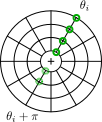
\includegraphics[width=0.5\textwidth]{fig/innerGhost}
    \caption{\textit{
The solid lines black lines represent the coordinate curves of a mesh with $4$ points in the $\rho$ direction (excluding the outermost ghost-point depicted with a dashed black line), and $8$ points in the $\theta$-direction.
The green solid circles represent the inner grid points at $\theta=\theta_i$, with the corresponding ghost-points at $\theta=\theta_i + \pi$ depicted as green dashed circles.
    }}
    \label{fig:innerRho}
\end{figure}
%
In this solution, the ghost-points for the innermost grid points in $\rho$ (those closest to the singularity) will be set to the value of the innermost grid point which lies $\theta + \pi$ away.
The next ghost-point will be set to the value of the second innermost internal point which lies $\theta + \pi$ away, and so on.
In this thesis, only one ghost-point is used.
With this method the second order FD stencil for the radial derivative becomes at the innermost point
%
\begin{align*}
    \L.\parti{f}{\rho}\R|_{\rho=\frac{\Delta \rho}{2}} \simeq
    \frac{-f\L(-\frac{\Delta \rho}{2}, \theta\R) + f\L(\frac{3\Delta \rho}{2}, \theta\R)}{2\Delta \rho}
    =
    \frac{-f\L(\frac{\Delta \rho}{2}, \theta+\pi\R) + f\L(\frac{3\Delta \rho}{2}, \theta\R)}{2\Delta \rho}.
\end{align*}
%
This method was used in \cite{Naulin2008}, and is shown to be second order accurate in \cref{sec:MES}.

\subsection{The inner boundary condition for \texorpdfstring{$\phi$}{the potential}}
\label{sec:innerPhiBC}
%
We also need an artificial ghost-point for the innermost point in $\rho$ for inversion method described in \cref{app:lapInv}.
As the inversion in the $\rho$ direction will be done for each mode, the method described in \cref{sec:ghostRhoDeriv} is not directly applicable.

Instead, we can set the inner ghost-point depending on the evenness of the mode.
If the mode is even, the mode under consideration would have the same value diametrically opposite of the innermost point.
Notice that this is true for every point at the same radius.
Hence, the ghost-point for the inner $\rho$ value is set to the same as the value at the innermost $\rho$.

If the mode is odd, the mode under consideration has different signs at diametrically opposite positions.
Thus, the ghost-point for the inner $\rho$ value is set to the negative of the value at the innermost $\rho$.
The method was first used in \cite{Naulin2008}, and is depicted in \cref{fig:BCLaplace}.
%
\begin{figure}[h!]
    \centering
    \begin{subfigure}[t]{0.5\textwidth}
        \centering
        \includegraphics[width=0.8\textwidth]{fig/mode_4}
        \caption{An even mode.}
    \end{subfigure}%
    \hfill
    \begin{subfigure}[t]{0.5\textwidth}
        \centering
        \includegraphics[width=0.8\textwidth]{fig/mode_5}
        \caption{An odd mode.}
    \end{subfigure}
    \caption{Two points diametrically opposite of each other has the same sign if the mode is even, but opposite signs if the mode is odd.
            The red solid line connects points diametrically opposite of each other.}
    \label{fig:BCLaplace}
\end{figure}

% \section{Spectral filtering}
%
In order to ensure that no aliasing will occur and create a numerical instability like the one mentioned in \cite{Phillips1959}, we must use a spectral filter in the periodic direction.
Although sufficiently high viscosities or diffusions can prevent aliasing (such that all the higher modes are damped out), they typically also damp on modes which we would like to include in our simulation.
One way to get around this is to use spectral filters.

\subsection{Orszag's 2/3 rule}
As mentioned in \cite{Orszag1971}, only the $2/3$ of the topmost modes leads to aliasing.
To see this, recall that only mode numbers equal to or less than $N/2$ can be represented exactly on a grid discretized with $N$ points \cite{Bracewell2000book}.
Next, consider two mode numbers $m_1$ and $m_2$ which adds up to a mode $m_3$.
If $m_3=m_1+m_2>N/2$, the mode will be intepredet as $m_1+m_2 - N$ (i.e. it will be aliased to the negative frequencies).
If we call $M$ the highest mode we can have which would not give aliasing, we must then require that
%
\begin{align*}
    m_1+m_2 - N &< -M\\
    M + M - N &< -M\\
    2M - N &< -M\\
    3M &<  N\\
    M &< \frac{N}{3}
\end{align*}
%
In order words, modes with mode number less than $N/3$ does not contribute to aliasing.
Hence the name $2/3$-rule as $M$ is $2/3$ of the Nyquist frequency $M < (2/3)(N/2)$.

Thus aliasing in this case is prevented if we set all modes with a mode number equal or above $N/3$ to zero.
As we see in the next section, this does not completely eliminate the aliasing in a cylinder, due to radial coupling.

\subsection{Radial coupling}
%
As terms like $\{\phi, f\}$ effectively advects modes of $f$ radially, we must ask ourselves what the smallest allowed wave length in the periodic dircetion is.
Since the circumference is given by $C=2\pi\rho$, and since the number of points in the periodic $\theta$-direction is constant, we see that resolution is limited by the shortest allowed wave length at the outermost radius $L_\rho$.
Let us now consider sinusoids on the form $\sin(kx)$, living on the circumference $C$ at radius $\rho$.
The wavenumber is then given by $k=\frac{2\pi m}{C}$, and thereby the wavelength by
%
\begin{align}
    \lambda = \frac{C}{m}.
    \label{eq:wavelen}
\end{align}
%
The smallest resolved wavelength on $\rho=L_\rho$, where $L_\rho$ is the outermost radius is given by the Nyquist frequency.
This gives the wavelength $\lambda_{\text{Nyquist}} = \frac{C_{L_\rho}}{n_\theta/2}$, where $n_\theta$ is the number of points in the $\theta$ direction.
However, the smallest wavelength which does not give aliasing is given by the $2/3$-rule, so that
%
\begin{align}
    \lambda_\min = \frac{C_{L_\rho}}{\frac{2}{3}\frac{n_\theta}{2}} = \frac{3C_{L_\rho}}{n_\theta}.
\end{align}
%
By rearranging \cref{eq:wavelen}, we find that the max allowed modenumber for the circumference $C$ at radius $\rho$ is
%
\begin{align}
    m_\max = \L\lfloor \frac{C}{\lambda_\min}\R\rfloor,
\end{align}
%
where $\lfloor \cdot \rfloor$ denotes the floor function.
Note that we take the floor as we are looking for the maximum allowed integer.

% \chapter{Verification of the numerics}
% \label{chap:verification}
% In order to find solutions which matches real life experiments (at least to a certain degree), we need to ensure ourselves that the assumption in our models are sound.
As important is it to check that the machinery handeling the numerical calculation is correctly implemented.
This can be done by code verification.

Quoting \cite{Dudson2016}

\blockquote{
Code verification is a process of checking that the chosen set of partial differential equations is solved correctly and consistently, and is a purely mathematical exercise.
Code verification is not concerned with verifying that the chosen numerical methods are appropriate for the chosen set of equations.
Code verification is also not concerned with testing the ability of a given model to explain experimental observations.
This testing is dealt with in the subsequent validation process.
}

Thus, a code can be verified numerically, but still fail to match the desired features of a real life experiment.
In other words, it would have passed the verification failed the validation.
If the code has succuessfully passed a validation test, but fails a verification test, the success of the validation is questionable.
The success of the validation in this case could have been a mere coincident.

The verification process is throughly discussed in \cite{Oberkampf2010book}, and more condensed for the method of manufactured solution (MMS) in \cite{Salari}.
Note that the verification process can be time consuming, and can be regarded as an artform in itself.
Luckly, a major part of the implemntation has already been verified in the BOUT++ framework using MMS in \cite{Dudson2016}.

After a quick introduction of the concept of truncation errors, the MMS process will be briefly presented in \cref{sec:MMS} before verification of additional implementations in the CELMA code is given in \cref{sec:MES}.

\section{Numerical errors}
%
Our derivative operators are discretized in order for them to operate on a discretized grid.
Doing so introduces an error, which depends on the order of approximation.
To use a concrete example, let us consider the simplest differential equation
%
\begin{align}
    \deri{f(x)}{x} = g(x)
    \label{ver:ode}
\end{align}
%
where $f(x)$ and $g(x)$ are arbitrary functions (not to be confused with the distribution function and a metric element).
We seek to solve \cref{ver:ode} for $f(x)$.

Let us find the simplest approximation of the derivative in an arbitrary grid point $x_0$.
We first Taylor expand $f(x)$ around $x_0$ and evaluate it in $x_0 + h$ (where $h$ is the grid spacing).
This gives
%
\begin{align*}
    f(x_0+h)
    = f(x_0)
    + h \L.\deri{f(x)}{x}\R|_{x=x_0}
    + \L.\frac{h^2}{2}\deri{^2f(x)}{x^2}\R|_{x=x_0}
    + \mathcal{O}(h^3)
\end{align*}
%
Subtraction of $f(x_0)$ and division by $h$ now yields the following approximation of the derivative
%
\begin{align*}
    \frac{f(x_0+h) - f(x_0)}{h}
    =  \L.\deri{f(x)}{x}\R|_{x=x_0}
    + \L.\frac{h}{2}\deri{^2f(x)}{x^2}\R|_{x=x_0}
    + \mathcal{O}(h^2)
\end{align*}
%
Hence, the local truncation error LTE we do in a single point by using this approximation is
%
\begin{align*}
    \|e_{\text{LTE}}\|
    =
    \L\|\frac{f(x_0+h) - f(x_0)}{h} - \L.\deri{f(x)}{x}\R|_{x=x_0}\R\|
    =
    \L\| \L.\frac{h}{2}\deri{^2f(x)}{x^2}\R|_{x=x_0} + \mathcal{O}(h^2)\R\|
\end{align*}
%
In other words it scales with the grid spacing $h$ to the first order.
The global error in some $L$-norm $n$ can be defined as
%
\begin{align*}
    \L\|\ve{e}\R\|_{L_n} =
    \L\|\ve{f}_{\text{true}} - \ve{f}_{\text{numeric}}\R\|_{L_n}
\end{align*}
%
% FIXME: LTE and global error
where $\ve{f}_{\text{true}}$ is an array of the analytic solution in each grid point, and $\ve{f}_{\text{numeric}}$ is an array of the solution obtained numerically.
From linear PDE theory we have that the global error should converge to the LTE order if the scheme is consistent (the LTE $\to 0$ as $h\to 0$) and numerically stable%
\footnote{Note that the definition of stability depends on the context, see \cite{Leveque2007book} for more details.}.
%
If convergence is observed, the implementation is verified.

\section{Method of Manufactured Solution}
\label{sec:MMS}
For most PDEs, the true solution $\ve{f}_{\text{true}}$ is not known in advance.
Sometimes a solution can be found in some special limits.
If convergence is found for these special cases, the code is not generally verified.
There could still be implementation mistakes (not discoverable in the limiting cases) which could have dire consequences when a more general solution is sought numerically.
One way to get around the problem is to manufacture a solution.

Assume that we have a set of nonlinear spatio-temporal PDEs we would like to solve for.
Let us call the variables evolved in time for $\ve{f}=\{\ve{u}_e, \ve{u}_i, n, \Om^D, T_e, \ldots\}$.
If there are no mixed spatial and temporal variables, we can write the set of nonlinear PDEs as
%
\begin{align}
  \parti{\ve{f}}{t} = F(\ve{f}) \RA \parti{\ve{f}}{t} - F(\ve{f}) = \ve{0}
  \label{ver:setOfPDE}
\end{align}
%
where $F(\cdot)$ is a nonlinear operator which contains the discretized spatial differential operators.
As stated above, we do not know a priori which $\ve{f}$ which satisfies \cref{ver:setOfPDE}.
Therefore we manufacture a set of functions $\ve{f}_M$ which does not satisfy \cref{ver:setOfPDE}, but rather
%
\begin{align*}
    \parti{\ve{f}_M}{t} - F(\ve{f}_M) = \ve{S}
\end{align*}
%
Note that $\ve{f}_M$ is an exact analytical solution of $\parti{\ve{f}}{t} = F(\ve{f}) + \ve{S}$.
We can therefore solve numerically $\parti{\ve{f}}{t} = F(\ve{f}) + \ve{S}$ for $\ve{f}$, and find the global error (for each variable $\ve{u}_e, \ve{u}_i, n, \Om^D, T_e, \ldots$ by
%
\begin{align*}
    \L\|\ve{e}\R\|_{L_n} =
    \L\|\ve{f}_{M} - \ve{f}_{\text{numeric}}\R\|_{L_n}
\end{align*}
%
One can now test if the global error show the expected order of convergence.
Note that $\ve{f}_M$ and the coefficients in the various terms in the PDEs does not need to be physical, but that in order to test all terms in this set of equations, the parameters of the simulation should be chosen so that the magnitude of each term are of a similar order of magnitude.

\section{Method of Exact Solution}
\label{sec:MES}
%

Since there are implementations in this thesis which is not covered by the BOUT++ framework (see \cref{chap:additionalImplementation} for details), these implementation should be verified as well.
All of these implementations are either differencing operators, extrapolations or integration operators where an exact analytic solution can be found.
Hence, one can use the approach of method of exact solutions (MES) to verify these operations, and there will be no need for manufacturing a solution.

Although it is simpler to perform MES than MMS, there are certain points one should be aware of.
Especially since we are dealing with a periodic domain with a singularity in the center.
Let us now call the function we are operating on with a discretized operator $D$ for $f(\rho,\theta,z)$.
Hence, the source $S$ is given by $D[f(\rho,\theta,z)]=S$, where $S$.
If we are to take derivatives in the $\rho$ direction, we must take care that
%
\vspace{0.5cm}
\begin{enumerate}[noitemsep,nolistsep]
    \item $f(\rho,\theta,z)$ must be of $\mathcal{C}^\infty$ along $\rho$, particularly at \item $f(\rho=0,\theta,z)$.%
    \begin{itemize}[noitemsep,nolistsep]
            \item This implies that the function must also be single valued in $f(\rho=0,\theta,z)$.
            \item Even though the coordinate system have a singularity in $f(\rho=0,\theta,z)$, the function may be continuous in a different coordinate system.
    \end{itemize}
  \item Boundary conditions in $\rho$ must be satisfied.
\end{enumerate}
\vspace{0.5cm}
%
If we are to take derivatives in the $\theta$ direction, we must take care that
%
\vspace{0.5cm}
\begin{enumerate}[noitemsep,nolistsep]
    \item $f(\rho,\theta,z)$ must be of $\mathcal{C}^\infty$ along $\theta$, particularly at $f(\rho,\theta=0,z)$ and $f(\rho,\theta=2\pi,z)$%
    \begin{itemize}[noitemsep,nolistsep]
            \item This implies that the function must also be periodic
    \end{itemize}
\end{enumerate}
\vspace{0.5cm}
%
Note that there are functions not fulfilling all the criteria that can give convergence.

\subsection{Derivative operators}
\label{sec:derOp}
%
We will in this section use the following notation, which is consistent with BOUT++ notation (see \cref{foot:BOUT++coord} in \cref{sec:clebschAlign})
%
\begin{itemize}[noitemsep]
    \item \texttt{DDX(f)} for the second order discretization of $\partial_\rho f$.
    \item \texttt{D2DX2(f)} for the second order discretization of $\partial^2_\rho f$.
    \item \texttt{DDZ(f)} for the spectral discretization of $\partial_\theta f$.
    \item \texttt{D2DZ2(f)} for the spectral discretization of $\partial^2_\theta f$.
\end{itemize}
%
A function which satisfies most of the criteria in \cref{sec:MES} is
%
\begin{align*}
    f(\rho, \theta, z)
    =& \sin\L(
        \frac{1}{\sqrt{2}}\rho[\cos(\theta)+\sin(\theta)]\frac{2\pi}{2L_\rho}
          \R)
      \\&
      \exp\L(
        -\frac{1}{2w^2}
            \L[\rho^2 + \rho_0^2 - 2\rho\rho_0(\cos[\theta - \theta_0])\R]
          \R)
      \\&
        \L(\frac{\rho\cos[\theta]+L_\rho}{2L_\rho}\R)^2,
        \numberthis
        \label{eq:MESf1}
\end{align*}
%
where
%
\begin{align*}
    &L_\rho = 30&
    &\text{
        Cylinder radius
    }&
    \\
    &w = \frac{4}{5}L_\rho&
    &\text{
        Width of Gaussian
    }&
    \\
    &\rho_0 = \frac{3}{10}L_\rho&
    &
    \rho
    \text{
        - coordinate for center of Gaussian
    }&
    \\
    &\theta_0 = \frac{5\pi}{4}&
    &
    \theta
    \text{
        - coordinate for center of Gaussian
    }&
\end{align*}
%
The function is depicted in \cref{fig:typicalMES}, and has the advantage that it is not symmetric across the axis.
However, it is not $\mathcal{C}^\infty$ in $\rho=0$, as the first derivative of the function (with respect to $\rho$) is multivalued there.
As a consequence it is found that for example \texttt{DDX(DDX(f))} diverges rather than converges when applying MES to \cref{eq:MESf1}%
%
\footnote{The ghost points are re-calculated after using the first operation on $f$.}
\footnote{Note that convergence is found for \cref{eq:MESf1} when using \texttt{D2DX2(f)}, and that convergence for \texttt{DDX(DDX(f))} is found using functions which are of $\mathcal{C}^\infty$, but which are not symmetric.\label{foot:DDXDDX}}
%
\begin{figure}[t!]
    \centering
    \begin{subfigure}[t]{0.45\textwidth}
        \centering
        \includegraphics[width=1.0\textwidth]{fig/f}
        \caption{Vizualisation of \cref{eq:MESf1}}
        \label{fig:typicalMES}
    \end{subfigure}%
    ~
    \begin{subfigure}[t]{0.45\textwidth}
        \centering
        \includegraphics[width=1.0\textwidth]{fig/err}
        \caption{Errors of \texttt{DDX(f)}, where $f$ is given in \cref{eq:MESf1}}
        \label{fig:errorsMES}
    \end{subfigure}
    ~
    \begin{subfigure}[t]{0.45\textwidth}
        \centering
        \includegraphics[width=1.0\textwidth]{fig/conv}
        \caption{Convergence rate of \texttt{DDX(f)}, where $f$ is given in \cref{eq:MESf1}}
    \end{subfigure}
    \caption{An example of functions and errors found when using MES.}
\end{figure}

\subsubsection{Single operators}
\label{sec:singleOp}
%
In order to check that the singularity is correctly implemented, we can check that \texttt{DDX(f)} is giving the expected order of convergence on \cref{eq:MESf1} as this is not symmetric.
The error of the operation for $2^{11}$ points is shown in \cref{fig:errorsMES}.
It is important to notice that the error is not dominating at one particular point, but is spread out over domain.
If the inner ghost point were incorreclty implemented, this would be detected by a localized high error around $\rho=0$, and it is expected that the correct order of convergence would not be found.
In addition, we would like to check the convergence of \texttt{D2DX2}, \texttt{DDZ} and \texttt{D2DZ2} as these are used in the $\div\L(g[\grad f]\R)$ operator, and in the $\ve{u}_E^2$ advection of $n$.
The results are given in \cref{tb:MESResults}.
We note that the derivatives in the $\rho$ direction gives the expected second order convergence.
We also see that although the derivatives in the $\theta$ direction seems not to be converging, the errors are quite small.
This is because machine precision is quickly reached.
That is, the loss of precision due to subtraction of two almost equal quantities becomes larger than the error from the discretization itself.
The behaviour is depicted in \cref{fig:divDDZ}.
%
\begin{figure}[htb]
    \centering
    \includegraphics[width=0.5\textwidth]{fig/divDDZ}
    \caption{\textit{
            Divergence due to loss of precision of the operator \texttt{DDZ(f)}.
        }}
    \label{fig:divDDZ}
\end{figure}
%
We therefore consider the schemes up until this point for convergent.

Finally, we will point out an important caveat.
Several operators used in the CELMA code can be written as $\rho^{-n}\partial_\rho f$, and care must be taken as the division by $\rho$ can appear to break the convergence.
In the case of $\frac{\texttt{DDX}(f)}{\rho}$, the loss of expected convergence rate can be explained by looking at the finite difference stencil.
We have that%
%
\footnote{
Found by Taylor expanding $f$ around $x_0$, evaluating it in $x+\Delta$ and subtracting it from the function Taylor expanded around $x_0$ and evaluated in $x-\Delta$. The final result is then divided by $2\Delta$
}
%
\begin{align*}
    \deri{f}{x} - \texttt{DDX}(f) =
    \frac{\Delta^2}{6}\deri{^2f}{x^2} + \mathcal{O}(\Delta^3),
\end{align*}
%
where $\Delta$ denotes the grid spacing as showin in \cref{fig:flatBC}.
As the boundaries lays half between the grid points, $\L.\rho\R|_{\text{Index}=1}=\frac{\Delta}{2}$
Thus, in this point, we have that
%
\begin{align*}
    \L.\frac{\deri{f}{x}}{\rho}\R|_{\text{Index}=1}
    - \L.\frac{\texttt{DDX}(f)}{\rho}\R|_{\text{Index}=1}
    = \frac{\Delta}{3}\deri{^2f}{x^2} + \mathcal{O}(\Delta^2)
\end{align*}
%
Thus for the first inner point, the scheme is only $1$st order convergent in $\Delta$.
As a function like $\rho$ is known to machine precision, this does not imply that the operator is incorreclty implemented, only that verfication of $\rho^{-n}\partial_\rho f$ throuhg MES is not suitable.

\subsubsection{The Naulin Solver}
%
For the Naulin Solver (described in \cref{sec:NaulinSolver}) we will use \cref{eq:MESf1} for $n$ and a cartesian Gaussian for $\phi$.
Specifically, we use
%
\begin{align}
\phi = \exp\L(-\frac{1}{2w^2}[\rho^2 + \rho_0^2 - 2\rho\rho_0\cos(\theta - \theta_0)] \R)
\label{eq:MESf2}
\end{align}
%
with
%
\begin{align*}
& w = \frac{1}{2}L_\rho &
& \rho_0 = \frac{1}{5}L_\rho &
& \theta_0 = \pi &
\end{align*}
%
for $n$%
\footnote{The same convergence rate was found if the functions were swapped.}%
.
The results are given in \cref{tb:MESResults}.
We note that the method seems to be non converging for when increasing the number of points in $\theta$.
However, since we are using an spectral discretization in the $\theta$-direction, the error drops rapidly.
As a result, the error arising from discretization in $\rho$ quickly becomes dominant even with high resultion in the $\rho$ direction.
Hence, we conclude that the method is convergent.

\subsubsection{Arakawa implementation of \texorpdfstring{$\ve{u}_E^2$}{the squared E cross B drift}}
%
We will now verify the implementation of the
%
\begin{align*}
    \{\ve{u}_E^2, n\}
    =
    \L\{\L(\partial_{\rho} \phi\R)^2+ \frac{1}{\rho^2}\L(\partial_{\theta} \phi\R)^2, n\R\}
    =
    \L\{\L(\partial_{\rho} \phi\R)^2,n\} + \{\frac{1}{\rho^2}\L(\partial_{\theta} \phi\R)^2, n\R\}
    .
\end{align*}
%
term, found in \cref{eq:ExBAdvImp}.
As the Arakwa implementation of $\{\phi,\cdot\}$ was found convergent using MMS in \cite{Dudson2016}, and because the treatment of the singularity was found to be convergent in \cref{sec:singleOp}, we would here like to check that ghost points are correctly calculated after doing the $\partial^2_\rho \phi$ operation.
Hence, we seek only to MES the term
%
\begin{align*}
    \L\{\L(\partial_{\rho} \phi\R)^2,n\R\}.
\end{align*}
%
As noted in \cref{foot:DDXDDX}, we should here find a different function for $\phi$ as the first derivative with respect to $\rho$ of \cref{eq:MESf1} has the problem that it is not single valued on the axis.
Instead, we will use the function
%
\begin{align*}
    \phi =& 10\L(6+\L[\frac{\rho}{L_\rho}\R]^3\R) \cos(2\theta)
    \\&
            \L(
                   \cos\L[2\pi\frac{\rho}{L_\rho}\R] + \sin\L[2\pi\frac{\rho}{L_\rho}\R]
                 + \cos\L[6\pi\frac{\rho}{L_\rho}\R] + \cos\L[4\pi\frac{\rho}{L_\rho}\R]
             \R)
    \\&
                \frac{1}{2}\L(1-\tanh\L[\frac{1}{8}\rho\R]\R)
                \numberthis
            \label{eq:arakawaUE}
\end{align*}
%
Note that since the Arakwa implementation does use fourier discretization, there is no problem that this function contains a sum of in $\theta$.
Thus we do not get the advantages of the spectral convergence rate.
However, the errors in the $\rho$ may dominate when successively making the grid spacing in $\theta$ smaller and vice versa.
This is what happens when performing the MES test in the $\theta$ direction, as seen in \cref{tb:MESResults}.
One could of course increased the resolution even more in $\rho$, but this would make the test significantly more computationally expensive.
Inspection of the error plot shows that the error is not dominating in any perticular point, and we can therefore conclude that the implementation is convergent.

Also note that we are not applying the MES to $\frac{1}{2\rho}\L\{\L(\partial_{\rho} \phi\R)^2,n\R\}$, as the $\frac{1}{\rho}$ factor reduces the convergence rate as mentioned in \cref{sec:singleOp}.

\subsection{Extrapolation to ghost points}
%
The verification of extrapolation to the outer ghost points in $\rho$ was verified in \cref{sec:derOp}.
What remains is to verify the parallel extrapolation of the ghost points for $\phi$, and to verify the sheath boundary condition for $j_{\|}$.
Notice that the polynomials in \cref{sec:extrapolGhost} are of fourth order.
This is to avoid propagation of one point errors when the ghost point is re-inserted in the FDA.
For the sheath boundary condition, the following functions are used
%
\begin{align}
    \phi =& \sin\L(\frac{1}{\sqrt{2}}[\rho + z]\frac{2\pi}{2L_\rho}\R)
    \label{eq:MESPhiSheath}
    \\
    n =& \cos\L(\frac{2\pi z}{L_z}\R)\sin^2\L(\frac{2\pi\rho}{L_\rho}\R)
    \label{eq:MESNSheath}
    \\
    u_{i, \|} =& \sin\L(\frac{z}{L_z}\R)\cos^2\L(2+2\pi\frac{\rho}{L_\rho}\R)
    \label{eq:MEUISheath}
\end{align}
%
Notice that $u_{e,\|}$ is given by the sheath boundary condition, and that this function does not need to be manufactured.
The result of the MES is given in \cref{tb:MESResults}.
% FIXME: If cauchy is used, include 3-cauchyBC

\subsection{Integration operators}
%
Finally the integration operators are verified.
Note that we are not using these routines when solving the set of PDEs, but to calculate the total particle number, the kinetic energy etc.
We now define the function
%
\begin{align*}
    H(d,s,c,w) = \frac{1}{2}\L(\tanh\L[s\L(d-\frac{c-w}{2}\R)\R]-\tanh\L[s\L(d-\frac{c-w}{2}\R)\R]\R)
\end{align*}
%
And use the following equations in the verification process
%
\begin{align}
f =& \frac{H\L(\rho, 2,\frac{L_\rho}{2}, \frac{L_\rho}{4}\R)}{\defi{0}{L_\rho}{H\L(\rho, 2,\frac{L_\rho}{2}, \frac{L_\rho}{4}\R)}{\rho}}
\label{eq:MESRhoInt}
\\
f =& \frac{H\L(\theta, 2,\pi, \frac{\pi}{2}\R)}{\defi{0}{2\pi}{H\L(\theta, 2,\pi, \frac{\pi}{2}\R)}{\theta}}
\label{eq:MESThetaInt}
\\
f =& \frac{H\L(z, 0.07,\frac{L_z}{2}, \frac{L_z}{4}\R)}{\defi{0}{L_z}{H\L(z, 0.07,\frac{L_z}{2}, \frac{L_z}{4}\R)}{z}}
\label{eq:MESZInt}
\end{align}
%
The results for each direction is given in \cref{tb:MESResults}.

\begin{landscape}
\subsection{Summary of convergence rates obtained}
\thispagestyle{empty}
% FIXME: Lines missing in this table, | and one \hline...is it correctly formatted? Check in a blank document
\begin{table}[h!]
{\footnotesize \centerline{
\colorme
\begin{tabular}{cccccccc}
\hline\hline
$\L.\R.$ \quad Operation                              \quad $\L.\R.$&
$\L.\R.$ \quad Direction                              \quad $\L.\R.$&
$\L.\R.$ \quad \scell{$L_\inf$}{order}                \quad $\L.\R.$&
$\L.\R.$ \quad \scell{$L_2$}{order}                   \quad $\L.\R.$&
$\L.\R.$ \quad \scell{$L_\inf$ error}{$2^{11}$ points}\quad $\L.\R.$&
$\L.\R.$ \quad \scell{$L_2$ error}{$2^{11}$ points}   \quad $\L.\R.$&
$\L.\R.$ \quad \scell{Equations}{used}                \quad $\L.\R.$&
$\L.\R.$ \quad Comment
\\
\hline
\hline
$\texttt{DDX}  (f)$         & $\rho$ & $2.00$ & $2.00$ & $1.99\cdot10^{-8}$ & $6.90\cdot10^{-9} $&\ref{eq:MESf1}&\\
$\texttt{D2DX2}(f)$         & $\rho$ & $2.00$ & $2.00$ & $1.58\cdot10^{-9}$ & $5.07\cdot10^{-10}$&\ref{eq:MESf1}&\\
$\frac{\texttt{DDX}(f)}{J}$ & $\rho$ & $1.00$ & $1.50$ & $3.16\cdot10^{-5}$ & $4.48\cdot10^{-7} $&\ref{eq:MESf1}&
\scell{No order $2$nd order convergence.}{Errors dominating close to $\rho=0$.}\\
$\texttt{DDZ}(f)$ & $\theta$ &  $-1.00$ & $-0.54$ & $9.12\cdot10^{-12}$ & $1.26\cdot10^{-13}$ & \ref{eq:MESf1}&
Machine precision reached.\\
$\texttt{D2DZ2}(f)$ & $\theta$ & $-1.99$ & $-1.57$ & $3.83\cdot10^{-9}$ & $6.65\cdot10^{-11}$ & \ref{eq:MESf1}&
Machine precision reached.\\
\scell{Naulin}{Solver} & $\rho$ & $2.00$ & $2.00$ & $3.19\cdot10^{-7}$ & $1.65\cdot10^{-7}$ & \ref{eq:MESf1} for $n$ and \ref{eq:MESf2} for $\phi$& $n_\theta=2^{12}$\\
\scell{Naulin}{Solver} & $\theta$ & $0.00$ & $0.00$ & $7.98\cdot10^{-9}$ & $4.13\cdot10^{-8}$ & \ref{eq:MESf1} for $n$ and \ref{eq:MESf2} for $\phi$ &
\scell{$n_\rho=2^{12}$, errors from}{$\rho$ discretization dominating}\\
$\L\{\L(\partial_{\rho} \phi\R)^2,n\R\}$ & $\rho$ & $2.00$ & $2.00$ & $1.60\cdot10^{-7}$ & $2.43\cdot10^{-8}$ & \ref{eq:MESf1} for $n$ and \ref{eq:arakawaUE} for $\phi$ & $n_\theta=2^{12}$\\
$\L\{\L(\partial_{\rho} \phi\R)^2,n\R\}$ & $\theta$ & $1.35$ & $1.46$ & $1.12\cdot10^{-8}$ & $8.41\cdot10^{-8}$ & \ref{eq:MESf1} for $n$ and \ref{eq:arakawaUE} for $\phi$ &
\scell{$n_\rho=2^{12}$}{Convergence found until $n_\theta=2^{9}$}\\
\scell{$\phi$}{$z$-extrapolation} & $z$ & $3.47$ & $4.50$ & $5.60\cdot10^{-16}$ & $5.86\cdot10^{-18}$ & \ref{eq:MESf1} & Machine precision reached.\\
\scell{$j_{\|}$}{sheath}          & $z$ & $3.98$ & $4.50$ & $2.38\cdot10^{-10}$ & $2.18\cdot10^{-12}$ & \scell{\ref{eq:MESPhiSheath} for $\phi$, \ref{eq:MESNSheath} for $n$}{and \ref{eq:MEUISheath} for $u_{i,\|}$}& \\
$\inde{f}{V}$  & $\rho$   & $2.01$ & $-$ & $3.50\cdot10^{-9} $ & $-$ &\ref{eq:MESRhoInt}  &$n_\theta= n_z     =512$\\
$\inde{f}{V}$  & $\theta$ & $2.21$ & $-$ & $2.03\cdot10^{-10}$ & $-$ &\ref{eq:MESThetaInt}&$n_\rho  = n_z     =512$\\
$\inde{f}{V}$  & $z$      & $2.00$ & $-$ & $2.01\cdot10^{-8}$ & $-$ &\ref{eq:MESZInt}    &$n_\rho  = n_\theta=512$\\
\hline\hline
\end{tabular}
}}
\caption[]{\textit{Results of the convergence tests}}
\protect\label{tb:MESResults}
\end{table}
\end{landscape}


\part{Numerical simulations}
Hang tight, the results will come soon
% FIXME: Insert the results here

\chapter{Simulation set up}
In this chapter the simulation setup will be discussed.
The domain size, the initial conditions and the source function will be defined, and the resolution will be given together with a discussion of the observed see-sawing pattern in $j_\|$.
How the simulations are executed will be explained, before the hardware used for the simulations is specified.
For the implementation parameters, see \cref{tb:artVisc,tb:timeSolve,tb:Naulin}.

\section{Domain size and normalizations}
%
We will in this thesis use a physical domain size similar to the size of CSDX \cite{Tynan2004a}.
That is, we will use a cylinder length of $L_z=2.8\m$ and a plasma radius of $L_\rho=8\cm$.
Note that the plasma radius is much less than the radius of the cylinder chassis.

These parameters can be tranlated to normalized units once we specify $T_{e,0}$, $m_i$ and $B_0$.
We will use $T_{e,0} = 2.5\eV$, the mass of singly ionized Argon as $m_i$, and let $B_0$ vary between $0.02$ and $0.1 \T$.
This sets the ion sound speed to $c_s \approx 2.46\; \text{km s}^{-1}$.
The ions cyclotron frequency to $\om_{ci}\approx 2.42 B \cdot 10^6 \T\s^{-1}$, i.e. $\om_{ci}$ is in the range of $48.4\kHz$ to $242\kHz$ for the specified magnetic field strengths.
Consequently, as we print the output to the files after every $t\om_{ci}$ %
\footnote{Note that the internal timestep from the adaptive time solver is usually much smaller.}%
%
, this gives an output every $1\s$ in physical units.
The specified $c_s$ and $\om_{ci}$ gives a hybrid radius of $\rho_s \approx 1.02B^{-1}\cdot10^{-3}\m\T^{-1}$, which with the specified magnetic field strengths will be in the range $5.08\cm$ to $1.02\cm$.

% FIXME: Is neutral in?
We will use a normalized density $n_0 = 1\cdot 10^{19} \m^{-3}$, and let the neutral density $n_n=0$ unless else is specified.
The numbers are summarized in \cref{tb:input,tb:inputVar}.
%
\begin{table}[!htb]
    \begin{minipage}{.45\linewidth}
      \centering
        \caption{Fixed simulation parameters.}
            \colorme
            \begin{tabular}{c|ll}
            \hline\hline
            %
            Variable & Value & Units\\
            \hline
            %
            $L_\rho$  & $0.08$              & $\m$              \\
            $L_z$     & $2.80$              & $\m$              \\
            $n_0$     & $1\cdot 10^{19}$    & $\m^{-3}$         \\
            $T_{e,0}$ & $2.5$               & $\eV$             \\
            $m_i$     & $6.63\cdot10^{-26}$ & $\kg$             \\
            $c_s$     & $2.46$              & $\text{km s}^{-1}$\\
            \hline\hline
            \end{tabular}
            \label{tb:input}
    \end{minipage}
    \hfill
    \begin{minipage}{.45\linewidth}
      \centering
        \caption{Variable simulation parameters.}
            \colorme
            \begin{tabular}{c|ll}
            \hline\hline
            %
            Variable & Range & Units\\
            \hline
            %
            $B_0$           & $0.02 - 0.01$  & $\T $ \\
            $\om_{ci}$      & $48.4 - 242$   & $\kHz$\\
            $\rho_s$        & $5.08 - 1.02$  & $\cm$ \\
            $L_\rho/\rho_s$ & $1.57 - 7.86$  &       \\
            $L_z/\rho_s$    & $55.0 - 275$   &       \\
            \hline\hline
            \end{tabular}
            \label{tb:inputVar}
    \end{minipage}
\end{table}

\section{Initial conditions and source specification}
\label{sec:initRun}
%
The coupled set of PDE's in \cref{eq:celma_vortD,eq:celma_dens,eq:celma_mom_dens,eq:celma_j_par,eq:celma_vortD_evolution} forms a  initial-boundary value problem.
The boundary conditions of this problem was given in \cref{sec:BCs}, but we have yet to define the initial conditions.

In the work presented here, we will use the following initial conditions of the normalized evolved quantities%
%
\footnote{$\Om$ is used rather than $\Om^D$ when simulating using the Boussinesq approximation}%
%
\begin{align*}
    &\ln(n)    = 0&
    &j_\|      = 0&
    &nu_{i,\|} = \frac{z}{L_z}&
    &\Om^D     = 0,&
\end{align*}
%
which will be used to find the steady state numerically as explained in \cref{sec:execution}.

Furthermore, we need to specify the source.
In this thesis, we have chosen the following shape of the source
%
\begin{align*}
    S = AH(\rho,s_{\text{profile}},c_{\text{profile}},w_{\text{profile}}),
\end{align*}
%
where $H$ is defined in \cref{eq:hat}, and $A=8.25\cdot10^{21} \m^{-3}\s^{-1}$ in physical units.
With this choice the normalized $n$ is around $1$ for $B=0.1\T$.
The arguments of $H$ are summarized in \cref{tb:source}, and $S$ is depicted in \cref{fig:parProfs,fig:radProfs}.
%
\begin{table}[!htb]
      \centering
        \caption{Source parameters used in the simulations.}
            \colorme
            \begin{tabular}{c|ll}
            \hline\hline
            %
            Variable & Value \\
            %
            \hline
            $s_{\text{profile}}$ & $5/L_\rho$\\
            $c_{\text{profile}}$ & $0$       \\
            $w_{\text{profile}}$ & $L_\rho$  \\
            \hline\hline
            \end{tabular}
            \label{tb:source}
\end{table}

Note that the source is uniform in along the parallel direction.
A more physical scenario would be to have a source decreasing in the parallel direction, before increasing around the SE due to recycling from the wall.
In any case, finding the proper shape of the source seems to be challenging, and is only accurate if detailed atomic physics is taken into account.
Although interesting and relevant, such atomic processes is outside the scope of this thesis.

\section{Resolution}
\label{sec:resolution}
%
In order to have a properly resolved grid, we need to properly resolve the gradient length scales.
From the point of computational time, a small number of grid points is preferable.
If we assume that the maximum gradient length scale from the model is around $\rho_s$, we should have $\frac{n_\rho}{L_\rho/\rho_s}>1$.
However, we have in this work found that $\frac{n_\rho}{L_\rho/\rho_s}\approx1$ can give simulation crashes, so a radial resolution of $\frac{n_\rho}{L_\rho/\rho_s}\approx3$ is aimed.
The same argument goes for the poloidal direction, where $L_\theta=2\pi L_\rho$.

As mentioned in \cref{chap:drift-order} the resolution in the parallel direction can be less since longer gradient scale lengths are found in the parallel direction as a consequence of the separation of scales.
The sheath sets the gradient scale length in the parallel direction, as will be explained in \cref{sec:parProf}.
Despite that the gradient scale sets a lower constraint on $n_z$, a see-sawing pattern is observed in simulations with a flow towards an end-plate for low $n_z$.
This problem has been observed in other plasma fluid codes dealing with sheath boundaries, but has to the authors best knowledge not been published.
For the work presented here, the problem is encountered for $j_\|$ as is illustrated in \cref{fig:see-saw}%
\footnote{It should be noted that running the simulations with odd number of points show similar behavior to what is presented in \cref{fig:see-saw}.}%
%
.
%
\begin{figure}[htb]
    \centering
    \includegraphics{fig/results/jParRipple006}
    \caption{See-saw oscillations for $B=0.06\T$ in the steady-state using $16, 24, 32, 42, 50$ and $66$ grid points in the parallel direction.
        $f$ is defined in \cref{eq:defF}
    }
    \label{fig:see-saw}
\end{figure}
%

\noindent
To get a better understanding of this behavior, the different terms in \cref{eq:celma_j_par} in the steady-state has been plotted in \cref{fig:jParBalance}.
%
\begin{figure}[htb]
    \centering
    \includegraphics{fig/results/jParBalanceNy66}
    \caption{The different terms making up \cref{eq:celma_j_par} in the steady-state for $n_z=66$ for $B=0.06$.
    }
    \label{fig:jParBalance}
\end{figure}
%
It is clear that the steady state is dominated by a balance between the Boltzmann response of the electrons and resistive terms.
This is also seen for lower $n_z$, albeit with stronger oscillations in the Boltzmann response and the resistive term for decreasing $n_z$.
As the resistive term is $\propto j_\|$ it cannot be the cause of the observed see-sawing.
Thus we can conclude that the see-sawing behavior comes from the difference between the logarithm of the density and the potential.

One could imagine that the see-sawing came from catastrophic cancellation between $\ln(n)$ and $\phi$.
If this was the case, the see-sawing would be even worse for an increased mass ratio $\mu$.
In fact, the opposite behavior is observed.
Running the simulations with $\text{H}$ gives more see-sawing than $\text{Ar}$.
The explanation can be found by looking at the fraction $f$ defined by
%
\begin{align}
    f \defined \frac{n_z}{L_z/\rho_s},
    \label{fig:defF}
\end{align}
%
which describes the resolution in terms of $\rho_s$.
We can now observe that
%
\begin{align*}
  f = \frac{n_zc_s}{L_z \om_{ci}}
    = \frac{n_z\sqrt{T_e}m_i}{\sqrt{m_i} L_z ZeB}
    = \frac{n_z\sqrt{T_em_i}}{L_z ZeB},
\end{align*}
%
i. e. it is proportional with $m_i$.
On this argument, running simulations with singly ionized $\text{Ar}$ gives a better resolution of $\sqrt{m_{\text{Ar}}/m_H}\approx6.3$ as compared with $\text{H}$.
That increased oscillations has been observed with simulations done with increasing $B$ and $L_z$ strengthens the hypothesis as $f\propto 1/BL_z$.

To keep the oscillations at a minimum, we require $f > 0.2$ in the simulations performed here, which sets a lower bound on $n_z$
Ideally, we would like to reduce the number of parallel points to speed up the simulations.
Therefore some alternative strategies to lower the grid-size oscillation is discussed in the following.

Increased artificial viscosity will alleviate the problem.
Unfortunately, it is found that the artificial viscosity coefficients needed for a smooth $j_\|$ makes the artificial viscosity term dominate, such that the steady state is defined by a balance between the Boltzmann terms, the resistive term and the artificial terms.
The same holds true if the artificial viscous terms are changed with hyperviscous terms of order $4$ (i.e. with $\partial_z^4$ terms).

To reformulate the problem into a finite volume problem seems to be a good idea as fluxes through the cell centers are conserved.
However, the same grid-size oscillation problem has been found in finite volume models \cite{Dudson2017Private}.

Finally, a split-scheme could lessen the problem.
Since the discretization of $n\mu\partial_z\L(\ln(n)-\phi\R)$ is done with a centered FD scheme, odd and even grid points will be decoupled.
That is, $\partial_z\L(\ln(n)-\phi\R)$ for odd grid points will only depend on the even points and vice versa.
For advective terms references \cite{Honein2004,Pirozzoli2011} suggest a skew-symmetric split in the form $\div\L(a\ve{u}\R) = \frac{1}{2}\L[\div\L(a\ve{u}\R) + a\div\ve{u} + \ve{u}\cdot\grad a\R]$ where all the right hand terms are discretized using centred difference schemes to get rid of the decoupling.
Although arising from a divergence term, rewriting
%
\begin{align*}
    n\mu\partial_z\L(\ln(n)-\phi\R) =
    \frac{1}{2}\L(
    \partial_z\L[n\mu\L(\ln(n)-\phi\R)\R]-\L[\ln(n)-\phi\R]\partial_z\L[n\mu\R]
    - n\mu\partial_z\L[\ln(n)-\phi\R]
    \R)
\end{align*}
%
may help for the grid-size oscillations.
This has, however, not been tried in the work presented in this thesis.

The grid size used in this thesis is given in \cref{tb:grid}.
%
\begin{table}[!htb]
      \centering
      \caption{Grid size used in the simulations.}
        \colorme
        \begin{tabular}{c|ll}
        \hline\hline
        %
        Variable & Value \\
        %
        \hline
        %
        $n_\rho$   & $32$  \\
        $n_z$      & $66$  \\
        $n_\theta$ & $256$ \\
        \hline\hline
        \end{tabular}
        \label{tb:grid}
\end{table}

\section{Simulation execution}
\label{sec:execution}
%
The simulations are executed in four steps.

First, The simulation is allowed to evolve freely to a steady-state condition using $n_\theta = 1$
This choice is justified by assuming axisymmetry.
A transient period with fast dynamics is observed before a slow settlement to the steady-state.
The steady-state is found by visual inspection, and is defined to be the time when there is a minimal difference between two time steps.
The steady-state is usually reached between $2000-3000t\om_{ci}$.
In order to ensure that the system has reached a steady state, the simulations are therefore runned to $4000t\om_{ci}$ .

Secondly, the simulation is expanded to $n_\theta = 256$, and runned for additional $50t\om_{ci}$ in order to ensure that the system is still in an axisymmetric steady state.

Thirdly a white noise perturbation with an amplitude of $1\cdot10^{-6}$ is added to $\Om^D$%
\footnote{Different approaches has been used for the perturbation.
    It should be noted that some of these gives a different route to the turbulent state (i.e. some perturbations dies out, while others have some intermediate non-linear steps before the linear growth rates), but gives (with very little difference) the same growth rates and the same statistical behavior of the saturated turbulence as the perturbation method stated.}
%
as this term is driving the non-linear advections through $\phi$.

If the system is unstable to small perturbations, and if there are no "crashes" in the simulation, a saturated turbulence state is eventually reached.

\section{Hardware}
%
All the simulations presented here are run on the \texttt{A1} (Broadwell) partition of the \texttt{Marconi} super cluster located at CINECA at Casalecchio di Reno (Bologna).
At the time of writing the cluster operated with the following specifications \cite{Marconi2016Web}
%
\begin{enumerate}[noitemsep]
    \item Model: Lenovo NeXtScale
    \item Architecture: Intel OmniPath Cluster
    \item Nodes: $1512$
    \item Processors: $2\times18$-cores Intel Xeon E$5-2697$ v$4$ (Broadwell) at $2.30$ GHz
    \item Cores: $36$ cores/node, $54432$ cores in total
    \item RAM: $128$ GB/node, $3.5$ GB/core
    \item Internal Network: Intel OmniPath Architecture $2$:$1$
    \item Disk Space: $17$PB (raw) of local storage
    \item Peak Performance: $2$ PFlop/s
\end{enumerate}
%
In all the simulations, $2$ nodes has been allocated using $48$ cores.
This has been found to give a good speed-up (as compared to use one node) with a good trade off between the ration of simulation time to communication time per core.

\chapter{Evolution of the plasma}
\section{The steady state}

The way to steady state described in
here remarks on the resulting profiles.

\subsection{Parallel profiles}
Consider: Remove ln(n), vortD, nui
%
\begin{figure}[htb]
    \centering
    \includegraphics[width=1.0\textwidth]{fig/results/1DProfiles/B010Par}
    \caption{Parallel profiles in the steady state for $B=0.1\T$}
    \label{fig:parProfs}
\end{figure}


Parallel
The parallel profile is mainly determined by the source, the sheath condition and the boundary condition at the sheath entrance.
There exsists a threshold on the source for which below the threshold the plasma is completely emptied and no density profile is allowed to build up.
Above this threshold the parallel extent of the source determines the filling.
That is:
The parallel shape of the source has less to do with the shape of the parallel density profile than the parallel extent of the source.
If the boundary condition on the density was changed to for example the Cauchy boundary condition (described in ...)
the shape of the steady state profile would be much steeper close to the sheath entrance.
Such steep gradients may give rise to numerical instabilities if the spatial resolution is not increased.

We observe that the potential profile follows the density profile quite well.
This is expected as to the first order the pressure is balancing the electric field, as seen in the ordering described in....
and because we do not restric the potential by any parallel boundary condition.

Next, the parallel velocity profiles are mainly arising from the parallel boundary condition.
Both the ions and electrons are fixed to a zero velocity at the boundary opposite to the sheath.
The ions are further fixed to the ion sound velocity at the sheath entrance, whereas the electron velocity will regulate itself after the potential.
If more electrons than ions were to escape, a potential difference would build up attracting more ions and pushing away more electrons.

Why is it not ambipolar?

Any difference in the velocities would lead to currents.
The divergence of current must be constant as a consequence of charge conservation.
Any parallel derivatives in the parallel current not balancing the other terms in ...
would lead to an acceleration of the plasma spinnig.

Therefore, the perpendicular vorticity profile comes as a direct consequence of the parallel derivative of the current in that point.

\subsection{Perpendicular profiles}

\begin{figure}[htb]
    \centering
    \includegraphics[width=1.0\textwidth]{fig/results/1DProfiles/B010Rad}
    \caption{Radial profiles in steady state for $B=0.1\T$}
    \label{fig:radProfs}
\end{figure}

Perpendicular profiles
As in the parallel direction, the shape of the perpendicular density profile is determined mainly by the source and the radial boundary conditions.
The radial extent of the source plays a larger role in determining the radial density profile than the shape of the source.

The perpendicular potential profile is a result of two effects.
Near the axis, the Boltzmann distribution follows induvidually for each radial position.
As we approach $L_\rho$ the radial potential profile will be effected by fixing the potential to $0$ at $L_\rho$.
This differs from the density profile because of the zero gradient enforcement on $n$ at $L_\rho$.

\section{The linear phase}
Linear phase, see growing and rotation.

Linear phase comes from unstabilities in linear set of equation.
No non-linearities are needed.
If only linear system, growth rates would continue forever.

Doesn't start by itself, but is seeded with a Gaussian noise with a level of on vortD
% FIXME; Could add arrow indicating direction of rotation
%
\begin{figure}[htbp]
    \centering
    \begin{subfigure}[h]{1.00\textwidth}
        \centering
        \includegraphics[width=1.0\textwidth]{fig/results/rotModes/n-perpPol-2D-fluct-0}
        \label{fig:rot1}
    \end{subfigure}%
    \\
    \begin{subfigure}[h]{1.00\textwidth}
        \centering
        \includegraphics[width=1.0\textwidth]{fig/results/rotModes/n-perpPol-2D-fluct-1}
        \label{fig:rot2}
    \end{subfigure}
    \\
    \begin{subfigure}[h]{1.00\textwidth}
        \centering
        \includegraphics[width=1.0\textwidth]{fig/results/rotModes/n-perpPol-2D-fluct-2}
        \label{fig:rot3}
    \end{subfigure}
    \caption{Rotation of modes}
\end{figure}
%
Dominating mode is dependent on $B$, also, parallel mode moves
%
\begin{figure}[htbp]
    \centering
    \begin{subfigure}[h]{1.00\textwidth}
        \centering
        \includegraphics[width=1.0\textwidth]{fig/results/modesDiffScanVals/B002}
        \caption{$B=0.02 \T$}
        \label{fig:B002}
    \end{subfigure}%
    \\
    \begin{subfigure}[h]{1.00\textwidth}
        \centering
        \includegraphics[width=1.0\textwidth]{fig/results/modesDiffScanVals/B004}
        \caption{$B=0.04 \T$}
        \label{fig:B004}
    \end{subfigure}
    \\
    \begin{subfigure}[h]{1.00\textwidth}
        \centering
        \includegraphics[width=1.0\textwidth]{fig/results/modesDiffScanVals/B006}
        \caption{$B=0.06 \T$}
        \label{fig:B006}
    \end{subfigure}
    \caption{Dominant mode depends on $B$}
\end{figure}
%
A more quantitative way to look at the linear phase is to plot the fourier modes at the position of the most unstable growth.
From theory, this coincides with the position of largest gradient.
As the abscissa is logarithmic, exponential grow will appear as straigth lines
%
\begin{figure}[htbp]
    \centering
    \begin{subfigure}[h]{1.00\textwidth}
        \centering
        \includegraphics[width=1.0\textwidth]{fig/results/fourierModes/stable}
        \label{fig:fourierStable}
        \caption{For $B=0.02\T$ the system is stable against perturbation}
    \end{subfigure}%
    \\
    \begin{subfigure}[h]{1.00\textwidth}
        \centering
        \includegraphics[width=1.0\textwidth]{fig/results/fourierModes/unstable}
        \label{fig:fourierUnstable}
        \caption{Growth rate leading to saturated turbulence for $B=0.1\T$}
    \end{subfigure}
    \caption{Time trace of the Fourier modes.}
\end{figure}
%
Can be summarized in growth rates plot
Assuming perturbation on the from $A\exp\L(i[k_\theta \theta - \L(i\Im[\om] + \Re[\om]\R) t]\R)$, where one can assure oneself that positive $\Im(\om)$ causes exponential growth, and a positive $\Re(\om)$ causes a counter-clockwise rotation of the perturbation if $\theta$ grows in the counter-clockwise direction, as the inverse wavelength $k_\theta$ stays constant.
%
\begin{figure}[htbp]
    \centering
    \begin{subfigure}[h]{1.00\textwidth}
        \centering
        \includegraphics[width=1.0\textwidth]{fig/results/growthRates/growthRatesB0}
        \label{fig:grB}
    \end{subfigure}%
    \\
    \begin{subfigure}[h]{1.00\textwidth}
        \centering
        \includegraphics[width=1.0\textwidth]{fig/results/growthRates/growthRatesB0ModeNr}
        \label{fig:grBModeNr}
    \end{subfigure}
    \caption{$B$-dependency on growth rates}
\end{figure}
%
Compare gr with analytic gr?
Why different?

\section{The turbulence phase}
At a certain point the growth of the linear modes becomes large for non-linear affects to occur.
Through the non-linearities, mode-mode coupling occurs, leading to a cascading of enstrophy (global integrated vorticity) and energy.
The radial displacement of fluid parcels is much more restricted than the movement along the field lines due to the magnetic field.
Consequently, the turbulence have a more a 2 dimensional character than a 3 dimensional character.
This is something which is also seen in atmospheric flows, and leads to an inverse cascading of enstrophy as vortex strecthing cannot occur.
In other words eddies tend to merge together to larger coherent structures.

Should maybe back this up with references etc.

The main part of the energy is still cascading towards the smaller structures in 2D turbulence.
At small enough scales the energy dissipates through diffusive processes.
The turbulence will reach a steady state once the input of energy through the source is balanced by the dissipation of energy.
On the transition from the linear phase to the turbulent phase a energy overshot is observed.
\begin{figure}[htb]
    \centering
    \includegraphics[width=1.0\textwidth]{fig/results/energyTrace/energyTraceB008}
    \caption{Time trace of the energy for $B=0.08$.}
    \label{fig:energyTrace008}
\end{figure}

As a consequence the eddies evolve at a faster phase, before the saturated turbulent state where eddies evolve at a slower rate, and the energy stays closer to the temporal mean (as seen in ...)
It is also important to observe that the fluctations can be big enough to push the plasma off center as observed in ...
%
\begin{figure}[htbp]
    \centering
    \begin{subfigure}[h]{1.00\textwidth}
        \centering
        \includegraphics[width=1.0\textwidth]{fig/results/2DTurbulence/steadyStateN}
        \caption{The plasma at the steady state.}
        \label{fig:2Dsteady}
    \end{subfigure}%
    \\
    \begin{subfigure}[h]{1.00\textwidth}
        \centering
        \includegraphics[width=1.0\textwidth]{fig/results/2DTurbulence/violentBurst}
        \caption{A violent burst is observed at the energy overshoot.}
        \label{fig:violentBurst}
    \end{subfigure}
    \\
    \begin{subfigure}[h]{1.00\textwidth}
        \centering
        \includegraphics[width=1.0\textwidth]{fig/results/2DTurbulence/offCenter}
        \caption{$B=0.06 \text{T}$}
        \label{fig:offcenter}
    \end{subfigure}
    \caption{Turbulent eddies are observed in the saturated turbulence state.
    Here shown for $B=0.1\T$}
\end{figure}
%
The fluctuations are no longer in an ordered pattern as they were in the linear phase, as shown in
%
\begin{figure}[htb]
    \centering
    \includegraphics[width=1.0\textwidth]{fig/results/2DTurbulence/fluct}
    \caption{Fluctations in the turbulent state for $B=0.1\T$}
    \label{fig:2DFluct}
\end{figure}
%

\chapter{Characteristics of the fluctuations}
% FIXME: Need reference
As seen from snapshots...the fluctuations can be quite strong, something which has also been observed experimentally.
This is in fact something which should be taken into account when modelling the plasma.
% FIXME: Need reference
Models like Hasegawa-Wakatani are doing a split between background and fluctuations.
There, the free energy in the background gradients are driving the fluctuations, and only the fluctuations are kept track of.
As long as the background fluctuations are not severely altering the background gradients, this is a good approximation.
On the other hand, when the background gradients are perturbed sufficiently by the perturbations, the drive for the fluctuations are also altered, and the fixed background approximation breaks down.
% FIXME: Need reference
Models like CYTO and CELMA does not do the separation of background and fluctuations, and one are with these models able to investigate how the fluctuations affect the background and not only the other way around.
We can do so by comparing the steady state profiles with the turbulent profiles.
A poloidal average and a temporal average containing the whole time series are done in order to get a good avergaged picture of the turbulent profile.
As apparent from figure \cref{fig:posOfFluct008} the background profiles are flattened by the turbulence.
%
\begin{figure}[htb]
    \centering
    \includegraphics[width=0.5\textwidth]{fig/results/posOfFluct/posOfFluctB008}
    \caption{Flattening of the profiles together with the position of the fluctuations for $B=0.08\T$.
        The shaded area represents the standard deviation.
    }
    \label{fig:posOfFluct008}
\end{figure}
%

FIXME: Consider to include the type of fluctuation present.
Mention Jassby position of fluctuations.
NOTE: INSERT LINEAR THEORY AND LOCATION OF FLUCTUATIONS


Further investigation of the turbulence can be done through investigation of the time traces.
%
\begin{figure}[htb]
    \centering
    \includegraphics[width=1.0\textwidth]{fig/results/combinedPlots/008T}
    \caption{Characteristics of the time traces of the fluctuations at three radial positions.}
    \label{fig:combinedPlots008}
\end{figure}
%
This is done in \cref{fig:combinedPlots008}.
Again, we can observe that the fluctuations are large in amplitude, and (from the power spectra density PSD) that several frequencies are present simultanously.
This behavior is captured by the probability density functions (PDF), which measures the chance to encounter a value within an infetesimal range, if a value at a random time is withdrawn from the time trace.
Consequentually, if all values are equally probable, the PDF will have a Gaussian shape.
Deviations from the Gaussian shape is usually measured by the statistical moments skewness%
%
\footnote{
    The skewness is a measure of the mass of the distribution.
    If the skewness is negative, the left tail of the distribution is bigger than the right.
    For a pure Gaussian the skewness is 0.
}
%
and kurtosis
%
\footnote{
    The kurtosis is a measure of extreme events present in the distribution.
    For a pure Gaussian the skewness is 3.
    If the kurtosis is less than 3 (platykurtic) the distribution produces fewer and less extreme outliers than a gaussian.
    If the kurtosis is greater than 3 (leptokurtic) there are more extreme outliners, and the tails approaches zero slower than a Gaussian.
}
%
.
Figure \cref{fig:skewKurt008} highligths how this varies with the radius.
%
\begin{figure}[htb]
    \centering
    \includegraphics[width=0.5\textwidth]{fig/results/skewKurt/008T}
    \caption{Radial variations of the skewness and excess kurtosis (the kurtosis $-3$).}
    \label{fig:skewKurt008}
\end{figure}
%
One can see that close to the center, it is more probable to encounter a large negative fluctuation than a positive fluctuation.
Then, for higher radii, large positive fluctuations becomes more and more frequent.
From the excess kurtosis, we can see that extreme events are less likely than in a Gaussian random process, whereas extreme events are almost twice as likely in the edge as in a Gaussian random process.

Finally it can be noted that the radial turbulent transport is mainly positive and even more intermittent than the fluctuations in density alone.

\chapter{Zonal flows}
2D PSD array
Averaged poloidal velocities

\chapter{Comparison with the boussinesq approximation}
In this chapter we will make a comparison between the simulation using the full set of CELMA equations (\textbf{C}ELMA-\textbf{F}ull, or simply CF), with the simulations using the Boussinesq approximation (\textbf{C}ELMA-\textbf{B}oussinesq, or simply CB).
We will see that the missing $n$ in the vorticity equation causes a difference in the parallel electron and ion flux, and that the energy will drift with time.

\section{Steady state profiles}
%
\begin{figure}[h]
    \centering
    \includegraphics{fig/results/compareBouss/1DProfRad001B}
    \caption{Radial steady state profiles with and without the Boussinesq approximation for $B_0=0.1\T$.
        Dots denotes the full simulation (but does not indicate the location of a grid point).
        Triangles denotes the simulation with the Boussinesq approximation (but does not indicate the location of a grid point).
        The units are the same as those used in \cref{fig:radProfs}.
    }
    \label{fig:compareBoussProfRad}
\end{figure}
%
If we start by comparing the steady state profiles, we can first note that any difference between the CF and the CB model lays in the vorticity equation.
The biggest difference between \cref{eq:celma_vortD_evolution} and \cref{eq:celma_vort_boussinesq} is how the density factor in the compression of the density times the ion polarization term is treated.
By using the Boussinesq approximation, we assumed that the mentioned $n$ was the same as a flat background $n_0$.
This $n_0$ then got normalized out, meaning that the $n$-dependency in this term disappeared.
As a result, we ended up with a source term in the CB model not present in the CF model since this term got canceled with the source term from the density equation which we "smuggled" inside the $\d_t^E$ operator in the CF case.
Finally, the $\ve{E}\times\ve{B}$ advection terms are different in the two cases.
These differences affect both the background profiles and the fluctuations.

Hence, it should come as no surprise that the radial vorticity profile has changed.
This is indicated in \cref{fig:compareBoussProfRad}, which shows the difference between the CF and CB simulation for $B=0.1\T$.
As the radial vorticity profiles changes, it will lead to changes in the radial potential profile%
%
\footnote{One could say that it is the potential which determines the vorticity through $\Om = \grad_\perp^2 \phi$, but since we are evolving the vorticity in time we are instead inverting the equation for $\phi$.
In that respect $\Om$ determines $\phi$.}%
%
.
The radial density profile stays roughly the same for the CF and CB case, which will be discussed in further detail below.
For the radial profile of the parallel currents we can observe that the CB case gives slower velocities when $\rho \to L_\rho$
This, in turn, makes small changes in the radial parallel current profile, but gives a more shallow approach as $\rho\to L_\rho$.
%
\begin{figure}[h]
    \centering
    \includegraphics{fig/results/compareBouss/1DProfPar001B}
    \caption{Parallel steady state profiles with and without the Boussinesq approximation for $B_0=0.1\T$.
        Dots denotes the full simulation (but does not indicate the location of a grid point).
        Triangles denotes the simulation with the Boussinesq approximation (but does not indicate the location of a grid point).
        The units are the same as those used in \cref{fig:parProfs}.
    }
    \label{fig:compareBoussProfPar}
\end{figure}
%

On the other hand, the parallel $j_\|$ profile has changed, as seen in \cref{fig:compareBoussProfPar}.
First of all, the see-sawing seen in the non-Boussinesq case seem to have disappeared.
Although the oscillating patterns in the parallel current is still there, they are much less pronounced due to the higher values of $j_\|$.
Secondly, the parallel current is around $5$ time larger in magnitude close to the sheath entrance.
This comes from the fact that the balancing terms in the vorticity equation has changed.
In the non-Boussinesq case, the $n$ in $\div(nu_{p,i})$ helped to reduce the terms in the modified vorticity, and thereby the parallel current as $n$ was lower closer to the sheath.
As mentioned above, this $n$ disappears when using the Boussinesq approximation, so it can no longer help to reduce the parallel current.
We can see that this change cannot have its origin in the $\ve{E}\times\ve{B}$ advection terms, as these are not active during the steady state since the $\phi$-field is axisymmetric.
Neither can it origin from the additional source term due to the lack of $n$ dependence.

The higher values of $j_\|$ in the CB case causes $\Omega$ to be shifted to a higher value.
For the CB case, $\Omega$ is approximately $1500 \s^{-1}$ and does no longer cross $0$.
In other words, the local rotation of the plasma is in the same direction for all radii.
Finally, it is worth noting that the system still follows a Boltzmann relation to a high degree, as is the case in the non-Boussinesq case.
This can also explain why the density profile in the CB case is almost the same as in the CF case in the radial direction, as the Boltzmann relation approximately holds for each magnetic field line.
%

\section{The linear state}
%
The change in the vorticity equation has a profound effect on the linear phase.
In the CF case, identifying the linear phase based on the definition given in \cref{chap:linear} was fairly straight forward.
In the CB case the time trace of the Fourier modes are a bit more complicated.
An example of this is shown in \cref{fig:FFTCompB}.
%
\begin{figure}[htbp]
    \centering
    \begin{subfigure}[h]{0.45\textwidth}
        \hspace*{-1cm}
        \centering
        \includegraphics{fig/results/compareBouss/FFT006}
        \caption{Without the Boussinesq approximation.}
        \label{fig:FFTWOB}
    \end{subfigure}%
    \hfill
    \begin{subfigure}[h]{0.45\textwidth}
        \hspace*{-1cm}
        \centering
        \includegraphics{fig/results/compareBouss/FFT006B}
        \caption{With the Boussinesq approximation.}
        \label{fig:FFTWB}
    \end{subfigure}
    \caption{The time trace of the absolute value of the Fourier modes for $B_0=0.06\T$ for the non-Boussinesq and the Boussinesq case at the position of maximum linear gradient.
    }
    \label{fig:FFTCompB}
\end{figure}
%
In the CF case (\cref{fig:FFTWOB}), the perturbations shows a clear exponential growth.
The intermediate phase between the linear phase and the saturated phase is relatively short.
The CB case (\cref{fig:FFTWB}) has a very short exponential growth after the initial perturbations have died out.
This is followed by a rather long phase where the modes at some times are growing, whilst at others decaying.
The final state for $B_0=0.06\T$ seems to be indeterminate.
Some modes are decaying, whereas the modes with the largest amplitudes are neither growing nor decaying.

Although challenging, we can still try to find the dispersion from the definition of the linear phase given in \cref{chap:linear}.
The result is given in \cref{fig:GRBM,fig:GRBB}.
%
\begin{figure}[htbp]
    \centering
    \begin{subfigure}[h]{0.45\textwidth}
        \centering
        \includegraphics{fig/results/compareBouss/growthRatesB0ModeNr}
        \caption{The growth rates and angular frequencies as a function of $B_0$.}
        \label{fig:GRBB}
    \end{subfigure}
    \hfill
    \begin{subfigure}[h]{0.45\textwidth}
        \centering
        \includegraphics{fig/results/compareBouss/growthRatesB0Bous}
        \caption{The growth rates and angular frequencies as a function of the mode number.}
        \label{fig:GRBM}
    \end{subfigure}%
    \caption{The growth rates and angular frequencies in the CB case.}
    \label{fig:GRB}
\end{figure}
%
From \cref{fig:GRBM}, we can see that the growth rates of the modes are still increasing with increasing $B$-field.
However, the maximum growth is observed in one mode-number less than compared with the CF case.
There is also a steeper decrease in the growth rates for higher mode numbers in the CR case.
We observe that the maximum growth rates for the individual $B$-fields is less than half of what it is in the CF case.
One should also emphasize that in the CB case, only $B_0 \geq 0.08\T$ reaches the saturated%
\footnote{As will be shown in \cref{sec:turbB}, the turbulence in the Boussinesq approximation does not really saturate in terms of energy.
    We will still refer to this state as "saturated" in the CB case to distinguish it from the intermediate turbulent phase preceding the linear state.
} %
%
turbulent state, compared with $B_0 \geq 0.06\T$ in the CF case.

The real part of the dispersion relation is also quite different from the CF case.
As in the CF case, the decaying modes is rotating in the ion diamagnetic direction, but with a rate almost $10$ times higher than compared with the CF case.
This trend ceases for mode $6$ and $7$, where the CB modes suddenly rotates strongly in the electron diamagnetic direction.
A bigger difference is that in the CB case, also $B_0 = 0.04\T$ rotates in the ion diamagnetic direction, and also exceeds the rotation velocity of the $B_0 = 0.02\T$ case.
Only $B_0 \geq 0.06\T$ shows rotation in the electron diamagnetic direction.
For these magnetic field strengths the rotation increases with increasing magnetic field strength (with exception of the highest modes in $B_0 = 0.06\T$, which rotates in the ion diamagnetic direction).
This is also what was found in the CF case.
% Consider: Explain why

\section{The turbulence phase}
\label{sec:turbB}
%
There is also a large difference between the Boussinesq and the non-Boussinesq case in the turbulent state.
When investigating the energy in \cref{fig:energies008B} we notice three things.
%
\begin{figure}[htb]
    \centering
    \includegraphics{fig/results/compareBouss/energies008B}
    \caption{Time trace of the energy for $B=0.08\T$ using the Boussinesq approximation.}
    \label{fig:energies008B}
\end{figure}
%
Firstly, in contrast to what is observed in simulations without the Boussinesq approximation, the energy is increasing in the linear phase (with exception of the parallel electron energy, which after close inspection actually shows a slight decrease in the linear phase).
For the potential energy, this means that the total number of particles in the system is increasing as the electron temperature and volume is constant.
If the density is increasing, this would also explain why the other energies are increasing as well.
The parallel electron energy can then only be decreasing if the parallel electron velocity is decreasing.

Next, the energy overshoot is absent for magnetic fields below $0.1\T$.
This fact can also be seen by visual inspection the temporal evolution of the fields.
The dynamics does not appear to be much faster during the onset of the turbulence then during the turbulent state.

Finally, the energy appears to be drifting to higher values with time.
The absolute values of the energies are of approximately same order as for the CF case.

Visual inspection of the fields shows that the eddies evolves slower in the turbulence phase as when compared to the non-Boussinesq case.
Whereas the plasma in the CF develops filamentary structures, these structures are less pronounced in the CB case, and the plasma as a whole appear to be more coherent.
The dynamics in the CB also develops at a slower pace, as can be seen by comparing \cref{fig:turbEv} with \cref{fig:turbBEv}.
%
{
\clearpage
\thispagestyle{empty}
\begin{figure}[htbp]
    \centering
    \begin{subfigure}[h]{1.00\textwidth}
        \centering
        \includegraphics{fig/results/compareBouss/evolution/n-perpPar-2D-0}
    \end{subfigure}%
    \\
    \begin{subfigure}[h]{1.00\textwidth}
        \centering
        \includegraphics{fig/results/compareBouss/evolution/n-perpPar-2D-1}
    \end{subfigure}
    \\
    \begin{subfigure}[h]{1.00\textwidth}
        \centering
        \includegraphics{fig/results/compareBouss/evolution/n-perpPar-2D-2}
    \end{subfigure}
    \caption{Evolution of the plasma in the saturated turbulence phase when using the Boussinesq approximation.
        Here shown for $B=0.1\T$.
        The $B$-field points into the paper, and the black dashed lines indicates the slicing of the opposite plot.
    }
    \label{fig:turbBEv}
\end{figure}
\clearpage
}
%

\subsection{Fluxes}
%
Related to the drift in the energies as a function of time is the particle flux in the system.
This is depicted in \cref{fig:fluxB0008}.
%
\begin{figure}[htb]
    \centering
    \includegraphics{fig/results/compareBouss/flux008B}
    \caption{Integrated flux for $B=0.08\T$ using the Boussinesq approximation.}
    \label{fig:fluxB0008}
\end{figure}
%
It is apparent that there are more ions than electrons being lost in the system.
As a consequence, the plasma will be negatively charged with time.
Moreover, the continuous charging of the plasma will at some point break the quasi-neutral assumption, which is one of the back-bone assumptions in the drift-fluid approximation, and therefore also in the CELMA model.
In other words, the Boussinesq approximation in the current form is not consistent with its own assumptions.

Besides this very important fact, we can observe that the parallel fluxes in the CB case is of the same order of magnitude as the CF case, with the CB ion flux exceeding that of the CF case.
Furthermore, the perpendicular flux is less than half of what it is in the CF case.
This is consistent with the observation of less filamentation of the plasma as mentioned above.


\section{Fluctuations}
%
The coherent rotation of the plasma structure is also apparent from the time traces and PDF of $n$, shown in \cref{fig:comb008B}.
%
\begin{figure}[htb]
    \centering
    \includegraphics{fig/results/compareBouss/comb008B}
    \caption{Time traces in three fixed positions around the maximum gradient for $B=0.08\T$.}
    \label{fig:comb008B}
\end{figure}
%
The time traces for the three positions are more periodic than what was observed in \cref{fig:combinedPlots008}, which hints to the fact that there may be some rotation going on in the plasma.
One can observe that the PDFs in \cref{fig:combinedPlots008} are more Gaussian-like, something which is supported by the observed skewness and kurtosis in \cref{fig:skewKurt008B}.
The CB case has a lower skewness coefficient compared to the CF case, and the kurtosis coefficient is even lower than for a Gaussian distribution.
This means that plasma bursts of plasma are less likely, and that the plasma stays more coherent.
%
\begin{figure}[htb]
    \centering
    \includegraphics{fig/results/compareBouss/skewKurt008B}
    \caption{Skewness and kurtosis for $B=0.1\T$ using the Boussinesq approximation.}
    \label{fig:skewKurt008B}
\end{figure}
%

Returning to \cref{fig:comb008B} and \cref{fig:combinedPlots008}, we note that in the CB case, the maximum of the power density spectrum is shifted to a higher frequency by a factor of approximately $3$, and falls off at a slightly faster rate than for the CF case.
The position of the maximum gradient is also shifted slightly outwards.

Furthermore, lower fluctuation amplitudes can be seen in \cref{fig:fluctProfiles01B} where the profiles are less flattened than in the CF case.
Outside the position of the absolute maximum gradient the density profile follows the steady state profile to a good degree.
Finally, the potential is shifted closer to the absolute maximum of the gradient in the steady state.
%
\begin{figure}[htb]
    \centering
    \includegraphics{fig/results/compareBouss/fluctProfiles01B}
    \caption{Steady state and averaged turbulent density profiles together with the radial distribution of the standard deviations of the fluctuations using the Boussinesq approximation with $B=0.1\T$.}
    \label{fig:fluctProfiles01B}
\end{figure}
%

\chapter{Neutral scan}
NOTE: Waiting for runs to finish
% NOTE: Could maybe redo the x-axis to 80 60 40 20 pct ionization.
% NOTE: Could add 0 pct?


% \part{Appendices}
% \appendix
% \chapter{Averages}
% \label{app:averages}
% %
We will here define the averages used in this thesis.
%
\section{Velocity average over the distribution function}
%
The weigthed velocity average of $A$ is defined as
%
\begin{align}
    \expt{A}_{f} \defined
        \frac{
            \defi{-\infty}{\infty}{Af_\a}{^3v}
        }{
            \defi{-\infty}{\infty}{f_\a}{^3v}
        }
    =
        \frac{\defi{-\infty}{\infty}{Af_\a}{^3v}}{n_\a}
    \label{app:distAvg}
\end{align}


\section{The poloidal average}
\label{sec:polAvg}
%
The poloidal average of $A$ is defined as
%
\begin{align*}
    \expt{f}_\theta \defined
        \frac{
            \defi{0}{2\pi}{fJ}{\theta}
        }{
            \defi{0}{2\pi}{J}{\theta}
        }
    =
        \frac{
            J\defi{0}{2\pi}{A}{\theta}
        }{
            J\defi{0}{2\pi}{}{\theta}
        }
    =
        \frac{\defi{0}{2\pi}{A}{\theta}}{2\pi}
\end{align*}
%
where we have used that the definition of the differential arc length (equation (2.5.46) in \cite{Dhaeseleer1991book}).

\section{The temporal average}
%
The temporal average of $A$ is defined as
%
\begin{align*}
    \expt{A}_t \defined
        \frac{
            \defi{t_1}{t_2}{A}{t}
        }{
            \defi{t_1}{t_2}{}{t}
        }
    =
        \frac{\defi{t_1}{t_2}{A}{t}}{t_2-t_1}
\end{align*}

%
% \chapter{Drift ordering}
% \label{app:DO}
% We will in this section look at big and small terms in the perpendicular momentum equation in \cref{eq:perp_mom_start}.
The motivation for this is to make a drift ordering similar to what is done in \cite{Fitzpatrick2014book}, and from this get algebraic equations for each order of the perpendicular velocities.
We will do so by looking at characteristic scales of the system.
Before starting, we will have a brief look at the definition of the gradient length scales and of the quasi-neutrality of the system.

\section{Gradient length scale}
When doing order of magnitude estimates%
\footnote{
    Easy, approximate ways to estimate some numbers within the same orders of magnitudes as we would have reached by doing a more correct and rigorous study.
}%
, and will therefore introduce the \emph{gradient length scale}.
The gradient scale length serves as an estimate for the size of $\grad$.
That is, it tells us over how large distances there are sharp gradients for a bounded, smooth function.
For a field $f$, the gradient length scale $L_f$ is defined as%
\footnote{
    Note that the inverse gradient length scale is often denoted $k$ in the literature.
    This make sense for for example plane wave perturbations, which happens to have $\frac{1}{L_f}=k$, where $k$ is the inverse wave number.
    However, in order to avoid ambiguity, we will in this thesis use $L_f$ for the gradient scale length.
}%
%
\begin{align}
    \frac{1}{L_f} \defined \frac{\|\max\{\operatorname{abs}(\grad f)\}\|}{\operatorname{abs}\L(f\bigg|_{\|\max\{\operatorname{abs}(\grad f)\}\|}\R)}
    \label{eq:lenScale}
\end{align}
%
i.e. short and sharp gradients in $f$ have a short $L_f$.
We can similarly define the temporal scale as
%
\begin{align}
    \om_f = \frac{1}{\tau_f} \defined \frac{\max\{\operatorname{abs}(\partial_t f)\}}{\operatorname{abs}\L(f\bigg|_{\max\{\operatorname{abs}(\partial_t f)\}}\R)}
    \label{eq:timeScale}
\end{align}
%
The definitions in \cref{eq:lenScale,eq:timeScale} are quite strict, and we will in this thesis use a more approximate estimate for the gradient length scale.
Thus, when referring to gradient length scales in this thesis, we will mean "typical" values for the gradient scale lengths, so that
%
\begin{align*}
    \grad \sim \frac{1}{L},
\end{align*}
%
where $\sim$ denotes "of same order".

\section{Quasi-neutrality}
\label{sec:qn}
To get the condition of whether the system is quasi-neutral or not, we can do an order of magnitude estimate comparison of $Zn_i$ and $Zn_i - n_e$.
We find that
%
\begin{align}
    \frac{Zn_i - n_e}{Zn_i} =
    \frac{e(Zn_i - n_e)}{eZn_i}
    =
    \frac{\e_0\div\ve{E}}{eZn_i}
    \sim
    \frac{\e_0\L|E\R|}{\L|L_E\R|eZn_i}
    \label{eq:quasiNeutral}
\end{align}
%
We can find an approximate expression for $E$ through Faraday's induction law:
%
\begin{align*}
    \curl\ve{E} =& -\partial_t B\\
    \frac{|E|}{|L_E|} \sim& \frac{|B|}{\tau_B}\\
    |E| \sim& \frac{|L_E||B|}{\tau_B}
\end{align*}
%
Inserting this in \cref{eq:quasiNeutral} yields
%
\begin{align*}
    \frac{Zn_i - n_e}{Zn_i}
    \sim
    \frac{\e_0 |L_E||B|}{|L_E| e Zn_i \tau_B}\frac{m_i Ze}{m_i Ze}
    =
    \frac{\om_{ci}\e_0}{Z e n_i\tau_B}\frac{m_i}{Z e}
    =
    \frac{\om_{ci}}{\tau_B\om_{pi}^2},
\end{align*}
%
where $\om_{pi}$ denotes the ion plasma frequency%
\footnote{This can be interpreted as something like the typical frequency the ions would oscillate with if the ions where perturbed in a completely quiescent plasma.}
%
.
We will now assume that the fastest time scales which can occur in our system is much slower than the ion cyclotron frequency.
If we therefore set $1/\tau_B\to\om_{ci}$, we get
%
\begin{align}
    \frac{Zn_i - n_e}{Zn_i}
    \simeq
    \frac{\om_{ci}^2}{\om_{pi}^2}
    =
    \frac{\om_{ci}^2}{\om_{pi}^2}
    \label{eq:quasiNCompare}
\end{align}
%
which for our interest is a quantity much smaller than $1$.
Equivalently, if we introduce the \emph{normalizing} ion sound speed%
%
\footnote{Although the real ion sound speed is given by $c_s=\sqrt{\frac{T_e+\gamma' T_i}{m_i}}\;\gamma'=\frac{N+2}{N}$ for $N$ degrees of freedom, we will in this thesis use the symbol $c_s$ for $\sqrt{\frac{T_e}{m_i}}$, as this term frequently pops up in the derivations.}
%
\begin{align*}
    c_s = \sqrt{\frac{T_e}{m_i}},
\end  {align*}
%
and the ion hybrid radius (the ion gyro radius at the electron temperature)
%
\begin{align*}
   \rho_s=\frac{c_s}{\om_{ci}},
\end  {align*}
%
\cref{eq:quasiNCompare} can be stated as
%
\begin{align*}
    \frac{Zn_i - n_e}{Zn_i}
    \simeq
    \frac{\om_{ci}^2}{\om_{pi}^2}
    =
    \frac{c_s^2\om_{ci}^2}{c_s^2\om_{pi}^2}
    =
    \frac{c_s^2}{\rho_s^2\om_{pi}^2}
    =
    \frac{\frac{T_e}{m_i}}{\rho_s^2\frac{n_iZ^2e^2}{m_i\e_0}}
    =
    \frac{\frac{T_e\e_0}{n_iZ^2e^2}}{\rho_s^2}
    =
    \frac{\lambda_D^2}{\rho_s^2},
\end{align*}
%
where $\lambda_D$ is the Debye length, which tells at what radius an isolated charge is effectively electrically shielded by surrounding charged particles.

In other words, the quasi-neutrality is just a statement of what scales we are looking at.
Note that this does not imply that there cannot be large electrical field throughout the plasma, rather that the left hand side of
%
\begin{align*}
    \frac{\div \ve{E}}{Zn_i} = \frac{e}{\e_0} \frac{Zn_i-n_e}{Zn_i}
\end{align*}
%
is small (as $e$ and $\e_0$ is of the same order of magnitude).
We therefore have
%
\begin{align*}
    n\simeq Zn_i \simeq n_e
\end{align*}

\section{The inertia term}
\label{sec:doInert}
The left hand side of \cref{eq:perp_mom_start} reads
%
\begin{align*}
&
 \frac{1}{\om_{c\a}}
 \L(
 \partial_t \ve{u}_{\a,\perp}
 + \L[\ve{u}_{\a,\perp}
 + \ve{u}_{\a,\|}\R]\cdot\grad\ve{u}_{\a,\perp}
 \R)
\\
 %
 %
 %
 =&
 \frac{1}{\om_{c\a}}
 \L(
 \partial_t \ve{u}_{\a,\perp}
 + \L[\ve{u}_{\a,\perp}
 + \ve{u}_{\a,\|}\R]\cdot\grad\ve{u}_{\a,\perp}
 \R)
 \\
 %
 %
 %
 =&
 \frac{1}{\om_{c\a}}
 \L(
 \partial_t \ve{u}_{\a,\perp}
 + \ve{u}_{\a,\perp}\cdot\grad_\perp\ve{u}_{\a,\perp}
 + \ve{u}_{\a,\|}\cdot\grad_\|\ve{u}_{\a,\perp}
 \R)
 \numberthis
 \label{eq:do_inertia}
\end{align*}
%
From this, we can withdraw a characteristic timescale of change of the perpendicular velocity, a characteristic gradient length scale and a characteristic perpendicular velocity.
We will use the notation for a field $f$
%
\begin{align*}
    f = f^c \wt{f}
\end{align*}
%
where the superscript $f^c$ denotes the characteristic size of $f$ so that $\wt{f}$ is of $\mathcal{O}(1)$.
If we now apply this on \cref{eq:do_inertia}, we get
%
\begin{align*}
    &
 \frac{1}{\om_{c\a}}
 \L(
 \om^c_{\a,\perp}u^c_{\a,\perp}
 \partial_{\wt{t}} \wt{\ve{u}}_{\a,\perp}
 + \frac{u_{\a,\perp}^{c}u_{\a,\perp}^{c}}{L_{\perp, u_{\a,\perp}}}
 \wt{\ve{u}}_{\a,\perp}\cdot\wt{\grad}_\perp\wt{\ve{u}}_{\a,\perp}
 + \frac{u^c_{\a,\perp}u^c_{\a,\|}}{L_{\|, u_{\a,\perp}}}
 \wt{\ve{u}}_{\a,\|}\cdot\wt{\grad}_\|\wt{\ve{u}}_{\a,\perp}
 \R)
 \\
 %
 %
 %
 =&
 \frac{u^c_{\a,\perp}}{\om_{c\a}}
 \L(
 \om^c_{\a,\perp}
 \partial_{\wt{t}} \wt{\ve{u}}_{\a,\perp}
 + \frac{u^c_{\a,\perp}}{L_{\perp, u_{\a,\perp}}}
 \wt{\ve{u}}_{\a,\perp}\cdot\wt{\grad}_\perp\wt{\ve{u}}_{\a,\perp}
 + \frac{u^c_{\a,\|}}{L_{\|, u_{\a,\perp}}}
 \wt{\ve{u}}_{\a,\|}\cdot\wt{\grad}_\|\wt{\ve{u}}_{\a,\perp}
 \R)
\end{align*}
%
We now relate the velocities to $c_s$, so that
%
\begin{align*}
    \lambda \defined \frac{u^c}{c^c_s}.
\end{align*}
%
Further, by using the ion hybrid radius, we get
%
\begin{align*}
    &
 \lambda_{u_{\a,\perp}}
 \frac{c^c_s}{\om_{c\a}}
 \L(
 \om^c_{\a,\perp}
 \partial_{\wt{t}} \wt{\ve{u}}_{\a,\perp}
 +
 \lambda_{u_{\a,\perp}}
 \frac{ c^c_s }{L_{\perp, u_{\a,\perp}}}
 \wt{\ve{u}}_{\a,\perp}\cdot\wt{\grad}_\perp\wt{\ve{u}}_{\a,\perp}
 +
 \lambda_{u_{\a,\|}}
 \frac{L_{\perp, u_{\a,\perp}}}{L_{\perp, u_{\a,\perp}}}
 \frac{c^c_s}{L_{\|, u_{\a,\perp}}}
 \wt{\ve{u}}_{\a,\|}\cdot\wt{\grad}_\|\wt{\ve{u}}_{\a,\perp}
 \R)
 \\
 %
 %
 %
 =&
 \lambda_{u_{\a,\perp}}
 \frac{c^c_s}{\om_{c\a}}
 \L(
 \om^c_{\a,\perp}
 \partial_{\wt{t}} \wt{\ve{u}}_{\a,\perp}
 +
 \lambda_{u_{\a,\perp}}
 \frac{ \rho^c_s }{L_{\perp, u_{\a,\perp}}}
 \om^c_{ci}
 \wt{\ve{u}}_{\a,\perp}\cdot\wt{\grad}_\perp\wt{\ve{u}}_{\a,\perp}
 +
 \lambda_{u_{\a,\|}}
 \frac{L_{\perp, u_{\a,\perp}}}{L_{\|, u_{\a,\perp}}}
 \frac{\rho^c_s}{L_{\perp, u_{\a,\perp}}}
 \om^c_{ci}
 \wt{\ve{u}}_{\a,\|}\cdot\wt{\grad}_\|\wt{\ve{u}}_{\a,\perp}
 \R)
\end{align*}
%
we will now assume that the scales for the ions and electrons are the same.
This is, we are constraining the system in the following way
%
\begin{align*}
    \lambda              &\sim \lambda_{u_{e,\perp}}  \sim \lambda_{u_{i,\perp}} \\
    \om^c                &\sim \om^c_{e,\perp}        \sim \om^c_{i,\perp}       \\
    L_{\perp, u_{\perp}} &\sim L_{\perp, u_{e,\perp}} \sim L_{\perp, u_{i,\perp}}\\
    L_{\|, u_{\perp}}    &\sim L_{\|, u_{e,\perp}}    \sim L_{\|, u_{i,\perp}}
\end{align*}
%
If we at the same time introduce
%
\begin{align*}
    \frac{ \rho^c_s }{L_{\perp, u_{\perp}}} \defined \gamma
\end{align*}
%
we get
%
\begin{align}
 \lambda
 \frac{c^c_s}{\om_{c\a}}
 \L(
 \om^c
 \partial_{\wt{t}} \wt{\ve{u}}_{\a,\perp}
 +
 \lambda
 \gamma
 \om^c_{ci}
 \wt{\ve{u}}_{\a,\perp}\cdot\wt{\grad}_\perp\wt{\ve{u}}_{\a,\perp}
 +
 \lambda_{u_{\a,\|}}
 \frac{L_{\perp, u_{\a,\perp}}}{L_{\|, u_{\a,\perp}}}
 \gamma
 \om^c_{ci}
 \wt{\ve{u}}_{\a,\|}\cdot\wt{\grad}_\|\wt{\ve{u}}_{\a,\perp}
 \R)
 \label{eq:doLHSAfterFirstConstraint}
\end{align}
%
In order for these terms to  be of the same order, we must have that
%
\begin{align*}
 \om^c                    &\sim \lambda \gamma \om^c_{ci}  \sim \lambda_{u_{\a,\|}} \frac{L_{\perp}}{L_{\|, u_{\perp}}} \gamma \om^c_{ci}
 \\
 \frac{\om^c}{\om^c_{ci}} &\sim \lambda \gamma             \sim \lambda_{u_{\a,\|}} \frac{L_{\perp}}{L_{\|, u_{\perp}}} \gamma
 \numberthis
 \label{eq:firstOrdering}
\end{align*}
%
If we assume low frequent turbulence, we must have that
%
\begin{align*}
    \frac{\om^c}{\om^c_{ci}} \defined \e \ll 1
\end{align*}
%
Comparing the two first terms in \cref{eq:firstOrdering} gives
%
\begin{align*}
 \frac{\om^c}{\om^c_{ci}}
 \sim&
 \lambda
 \gamma
 \\
 \e
 \sim&
 \lambda
 \gamma
\end{align*}
%
in order to have a balanced restriction between gradient scale lengths and velocities, we can set
%
\begin{align*}
 \lambda
 \sim&
 \sqrt{\e}
 \\
 \gamma
 \sim&
 \sqrt{\e}
\end{align*}
%
note that if we would have started our constraint by saying $\sqrt{\e}\ll 1$ instead, the non-linear terms would be negligible.

Finally, we put the restriction on the parallel velocity and scale lengths.
We now define
%
\begin{align*}
\frac{L_{\perp}}{L_{\|, u_{\a,\perp}}}\defined \zeta
\end{align*}
%
By assuming $u^c_{\a,\|}\sim c^c_s$, and that
%
\begin{align*}
\zeta\sim \sqrt{\e},
\end{align*}
%
we find that
%
\begin{align*}
 \lambda_{u_{\a,\|}}
 \frac{L_{\perp}}{L_{\|, u_{\a,\perp}}}
 \gamma
 =
 \lambda_{u_{\a,\|}}
 \zeta
 \gamma
 \sim
 1\sqrt{\e}^2
 =
 \e
\end{align*}
%
This means that the left hand side of \cref{eq:perp_mom_start} can in an order of magnitude estimate be wirtten as (assuming that $\om_{c\a}\sim\om^c_{c\a}$
%
\begin{align*}
 &
 \lambda
 \frac{m_i}{m_i}
 \frac{c^c_s}{\om^c_{c\a}}
 \L(
 \om^c
 \partial_{\wt{t}} \wt{\ve{u}}_{\a,\perp}
 +
 \lambda
 \gamma
 \om^c_{ci}
 \wt{\ve{u}}_{\a,\perp}\cdot\wt{\grad}_\perp\wt{\ve{u}}_{\a,\perp}
 +
 \lambda_{u_{\a,\|}} \frac{L_{\perp, u_{\a,\perp}}}{L_{\|, u_{\a,\perp}}}
 \gamma
 \om^c_{ci}
 \wt{\ve{u}}_{\a,\|}\cdot\wt{\grad}_\|\wt{\ve{u}}_{\a,\perp}
 \R)
 \\
 %
 %
 &=
 \lambda
 \frac{m_\a}{m_i}
 \frac{c^c_s}{\om^c_{ci}}
 \L(
 \om^c
 \partial_{\wt{t}} \wt{\ve{u}}_{\a,\perp}
 +
 \e
 \om^c_{ci}
 \wt{\ve{u}}_{\a,\perp}\cdot\wt{\grad}_\perp\wt{\ve{u}}_{\a,\perp}
 +
 \e
 \om^c_{ci}
 \wt{\ve{u}}_{\a,\|}\cdot\wt{\grad}_\|\wt{\ve{u}}_{\a,\perp}
 \R)
 \\
 %
 %
 &=
 \lambda
 \frac{m_\a}{m_i}
 c^c_s
 \L(
 \frac{\om^c}{\om_{ci}}
 \partial_{\wt{t}} \wt{\ve{u}}_{\a,\perp}
 +
 \e
 \wt{\ve{u}}_{\a,\perp}\cdot\wt{\grad}_\perp\wt{\ve{u}}_{\a,\perp}
 +
 \e
 \wt{\ve{u}}_{\a,\|}\cdot\wt{\grad}_\|\wt{\ve{u}}_{\a,\perp}
 \R)
 \\
 %
 %
 &=
 \lambda
 c^c_s
 \frac{m_\a}{m_i}
 \e
 \L(
 \partial_{\wt{t}} \wt{\ve{u}}_{\a,\perp}
 +
 \wt{\ve{u}}_{\a,\perp}\cdot\wt{\grad}_\perp\wt{\ve{u}}_{\a,\perp}
 +
 \wt{\ve{u}}_{\a,\|}\cdot\wt{\grad}_\|\wt{\ve{u}}_{\a,\perp}
 \R)
 \\
 %
 %
 &=
 \lambda c^c_s \frac{m_\a}{m_i}
 \e
 \wt{\d}^\a_t\wt{\ve{u}}_{\a,\perp}
 \numberthis
 \label{eq:doInertiaEps}
\end{align*}
%

\section{Pressure, electric field and perpendicular velocities}
\label{sec:pep}
%
We will now group the three next terms in \cref{eq:perp_mom_start}, and we will in the end see that these have the same order under the right assumptions.
We have that
%
\begin{align*}
- \frac{ \grad_\perp p_\a }{n_\a  q_\a B}
+ \frac{\ve{E}_\perp}{B}
+ \ve{u}_{\a,\perp}\times\ve{b}
=&
- \frac{n^c T^c_\a}{L_{\perp, p_\a}n^cq_\a B^c}
\frac{ \wt{\grad}_\perp \wt{p}_\a }{\wt{n}_\a \wt{B}}
+ \frac{E_\perp^c}{B^c}
\frac{\wt{\ve{E}}_\perp}{\wt{B}}
+ \ve{u}^c_{\a,\perp}
\wt{\ve{u}}_{\a,\perp}\times\ve{b}
\\
%
%
=&
- \frac{T^c_\a}{L_{\perp, p_\a}q_\a B^c}
\frac{ \wt{\grad}_\perp \wt{p}_\a }{\wt{n}_\a \wt{B}}
+ \frac{E_\perp^c}{B^c}
\frac{\wt{\ve{E}}_\perp}{\wt{B}}
+\lambda c^c_s
\wt{\ve{u}}_{\a,\perp}\times\ve{b}
\numberthis
\label{eq:doTriple}
\end{align*}
%
We will now constrain the system further by saying that
%
\begin{align*}
L_{\perp} \sim& L_{\perp, p_\a} \sim L_{\perp, u_{\perp}}\\
T^c       \sim& T^c_e           \sim T^c_i
\end{align*}
%
This means that $c^c_s = \sqrt{\frac{T^c}{m_i}}$.
Using this in \cref{eq:doTriple} gives
%
\begin{align*}
-
\frac{m_i}{m_i}
\frac{T^c}{q_\a B^c}
\frac{1}{L_{\perp}}
\frac{ \wt{\grad}_\perp \wt{p}_\a }{\wt{n}_\a \wt{B}}
+ \frac{E_\perp^c}{B^c}
\frac{\wt{\ve{E}}_\perp}{\wt{B}}
+\lambda c^c_s
\wt{\ve{u}}_{\a,\perp}\times\ve{b}
%
%
=&
-
(c^c_s)^2
\frac{q_i}{q_\a}
\frac{1}{\om^c_{ci}}
\frac{1}{L_{\perp}}
\frac{ \wt{\grad}_\perp \wt{p}_\a }{\wt{n}_\a \wt{B}}
+ \frac{E_\perp^c}{B^c}
\frac{\wt{\ve{E}}_\perp}{\wt{B}}
+\lambda c^c_s
\wt{\ve{u}}_{\a,\perp}\times\ve{b}
\\
%
%
=&
-
c^c_s
\frac{q_i}{q_\a}
\frac{c^c_s}{\om^c_{ci}}
\frac{1}{L_{\perp}}
\frac{ \wt{\grad}_\perp \wt{p}_\a }{\wt{n}_\a \wt{B}}
+ \frac{E_\perp^c}{B^c}
\frac{\wt{\ve{E}}_\perp}{\wt{B}}
+\lambda c^c_s
\wt{\ve{u}}_{\a,\perp}\times\ve{b}
\\
%
%
=&
-
c^c_s
\frac{q_i}{q_\a}
\frac{\rho^c_s}{L_{\perp}}
\frac{ \wt{\grad}_\perp \wt{p}_\a }{\wt{n}_\a \wt{B}}
+ \frac{E_\perp^c}{B^c}
\frac{\wt{\ve{E}}_\perp}{\wt{B}}
+\lambda c^c_s
\wt{\ve{u}}_{\a,\perp}\times\ve{b}
\\
%
%
=&
-
c^c_s
\frac{q_i}{q_\a}
\gamma
\frac{ \wt{\grad}_\perp \wt{p}_\a }{\wt{n}_\a \wt{B}}
+ \frac{E_\perp^c}{B^c}
\frac{\wt{\ve{E}}_\perp}{\wt{B}}
+\lambda c^c_s
\wt{\ve{u}}_{\a,\perp}\times\ve{b}
\numberthis
\label{eq:doTripleToEps}
\end{align*}
%
For these to be of the same order, we must have
%
\begin{align*}
    \gamma c^c_s &\sim \frac{E_\perp^c}{B^c} \sim \lambda c^c_s \\
    \gamma     &\sim \frac{E_\perp^c}{c^c_sB^c} \sim \lambda
\end{align*}
%
this gives
%
\begin{align*}
    \Xi \defined \frac{E_\perp^c}{c^c_sB^c} \sim \sqrt{\e}
\end{align*}
%
Inserting this in \cref{eq:doTripleToEps} yields
%
\begin{align*}
-
c^c_s
\frac{q_i}{q_\a}
\gamma
\frac{ \wt{\grad}_\perp \wt{p}_\a }{\wt{n}_\a \wt{B}}
+ \frac{c^c_s}{c^c_s}\frac{E_\perp^c}{B^c}
\frac{\wt{\ve{E}}_\perp}{\wt{B}}
+\lambda c^c_s
\wt{\ve{u}}_{\a,\perp}\times\ve{b}
=&
-
c^c_s
\L(
\gamma
\frac{q_i}{q_\a}
\frac{ \wt{\grad}_\perp \wt{p}_\a }{\wt{n}_\a \wt{B}}
+ \frac{1}{c^c_s}\frac{E_\perp^c}{B^c}
\frac{\wt{\ve{E}}_\perp}{\wt{B}}
+\lambda
\wt{\ve{u}}_{\a,\perp}\times\ve{b}
\R)
\\
%
%
=&
-
c^c_s
\sqrt{\e}
\L(
\frac{q_i}{q_\a}
\frac{ \wt{\grad}_\perp \wt{p}_\a }{\wt{n}_\a \wt{B}}
+
\frac{\wt{\ve{E}}_\perp}{\wt{B}}
+
\wt{\ve{u}}_{\a,\perp}\times\ve{b}
\R)
\end{align*}

\section{Collisionalities and sources}
%
Next, we look at the collisionalities and sources of \cref{eq:perp_mom_start}.
We would like these to be (at maximum) of the same order of magnitude as the inertia terms of \cref{sec:doInert}.
Before we start, we will assume quasi-neutrality%
\footnote{This is discussed further in \cref{sec:qn}}%
%
, i.e.
%
\begin{align*}
    n\sim n_e \sim Zn_i
\end{align*}
%

\subsection{Coulomb collisions}
%
For the electron-ion collisionalities, we find
%
\begin{align*}
\frac{ \ve{R}_{\beta \to \a,\perp} }{n_\a q_\a B}
=&
\frac{ m_en_e\nu_{ei}\L(\ve{u}_{e,\perp}-\ve{u}_{i,\perp}\R) }{n_\a q_\a B}
\\
%
%
=&
\frac{m_e\nu^c_{ei}\lambda c^c_sn^c}{q_\a n^cB^c}
\frac{ \wt{n}_\a \wt{\nu}_{ei}\L(\wt{\ve{u}}_{e,\perp}-\wt{\ve{u}}_{i,\perp}\R) }{\wt{n}_\a \wt{B}}
\\
%
%
=&
\lambda c^c_s
\frac{m_iq_i}{m_iq_i}\frac{ m_e}{q_\a B^c} \nu^c_{ei}\frac{\wt{\ve{R}}_{\beta \to \a,\perp} }{\wt{n}_\a \wt{B}}
\\
%
%
=&
\lambda c^c_s
\frac{q_i}{q_\a}
\frac{m_e}{m_i}
\frac{\nu^c_{ei}}{\om^c_{ci}}
\frac{\wt{\ve{R}}_{\beta \to \a,\perp} }{\wt{n}_\a \wt{B}}
\\
%
%
=&
\lambda c^c_s
\frac{q_i}{q_\a}
\frac{1}{\mu}
\frac{\nu^c_{ei}}{\om^c_{ci}}
\frac{\wt{\ve{R}}_{\beta \to \a,\perp} }{\wt{n}_\a \wt{B}}
\numberthis
\label{eq:doRes}
\end{align*}
%
We will now set the ordering condition according to the ions.
If the ion equation of \cref{eq:doRes} is to be at the same order as the ion equation of \cref{eq:doInertiaEps} we get the condition
%
\begin{align*}
 \frac{1}{\mu}\frac{\nu^c_{ei}}{\om^c_{ci}}\lambda c^c_s \sim& \lambda c^c_s \e
 \\
 \xi\defined\frac{1}{\mu} \frac{\nu^c_{ei}}{\om^c_{ci}}           \sim& \e
\end{align*}
%
Where we have used that the masses in \cref{eq:doInertiaEps} cancels, and as all the terms with tilde are of order $\mathcal{O}(1)$
%
\cref{eq:doRes} can therefore be written as
%
\begin{align*}
\frac{ \ve{R}_{\beta \to \a,\perp} }{n_\a q_\a B}
\sim&
\lambda c^c_s
\frac{q_i}{q_\a}
\xi
\frac{\wt{\ve{R}}_{\beta \to \a,\perp} }{\wt{n}_\a \wt{B}}
\end{align*}

\subsection{Neutral collisions}
%
For the neutral collisions, we find that
%
\begin{align*}
\frac{ \ve{R}_{n \to \a,\perp} }{n_\a q_\a B}
=&
\frac{ m_\a n_\a \nu_{\a n} \ve{u}_{\a,\perp}}{n_\a q_\a B}
\note{Quasi-neutrality}
\\
=&
\frac{ m_\a n^c }{n^c q_\a B^c}\nu^c_{\a n} \lambda c^c_s
\frac{\wt{n}_\a \wt{\nu}_{\a n}\wt{\ve{u}}_{\a,\perp} }{\wt{n}_\a  \wt{B}}
\\
=&
\frac{m_iq_i}{m_iq_i}
\frac{ m_\a }{ q_\a B^c}\nu^c_{\a n} \lambda c^c_s
\frac{\wt{\ve{R}}_{n \to \a,\perp}  }{\wt{n}_\a  \wt{B}}
\\
=&
\frac{q_i}{q_\a}
\frac{m_\a}{m_i}
\frac{\nu^c_{\a n}}{\om^c_{ci}} \lambda c^c_s
\frac{\wt{\ve{R}}_{n \to \a,\perp} }{\wt{n}_\a  \wt{B}}
\end{align*}
%
We will now try to relate $\nu^c_{e n}$ to $\nu^c_{i n}$.
From \cref{app:collisions} we have that
%
\begin{align*}
    &\nu_{en} \propto \frac{n_n a_0^2 \sqrt{T_e}}{\sqrt{m_e}}&
    &\nu_{in} \propto \frac{n_n a_0^2 \sqrt{T_i}}{\sqrt{m_i}}&
\end{align*}
%
As we have that $T_e \sim T_i$, we get
%
\begin{align*}
    \nu_{en} \propto& \frac{\sqrt{m_i}}{\sqrt{m_i}}\frac{n_n a_0^2 \sqrt{T_e}}{\sqrt{m_e}}\\
    \propto& \frac{\sqrt{m_i}}{\sqrt{m_e}}\frac{n_n a_0^2 \sqrt{T_e}}{\sqrt{m_i}}\\
    \sim   & \frac{\sqrt{m_i}}{\sqrt{m_e}}\nu_{in}
\end{align*}
%
This gives
%
\begin{align*}
    \frac{q_i}{q_\a}
    \frac{m_\a}{m_i}
    \frac{\sqrt{m_i}}{\sqrt{m_i}}
    \frac{\nu^c_{\a n}}{\om^c_{ci}} \lambda c^c_s
    \frac{\wt{\ve{R}}_{n \to \a,\perp} }{\wt{n}_\a  \wt{B}}
    \sim
    \frac{q_i}{q_\a}
    \frac{m_\a}{m_i}
    \frac{\sqrt{m_i}}{\sqrt{m_\a}}
    \frac{\nu^c_{i n}}{\om^c_{ci}} \lambda c^c_s
    \frac{\wt{\ve{R}}_{n \to \a,\perp} }{\wt{n}_\a  \wt{B}}
    \\
    %
    =
    \frac{q_i}{q_\a}
    \frac{\sqrt{m_\a}}{\sqrt{m_i}}
    \frac{\nu^c_{i n}}{\om^c_{ci}} \lambda c^c_s
    \frac{\wt{\ve{R}}_{n \to \a,\perp} }{\wt{n}_\a  \wt{B}}
    \numberthis
    \label{eq:doNeut}
\end{align*}
%
Again, we can do an ordering condition according to the ions.
The ion equation of \cref{eq:doNeut} is of the same order as the ion equation of \cref{eq:doInertiaEps} when
%
\begin{align*}
    \lambda c^c_s \e \sim& \frac{\nu^c_{i n}}{\om^c_{ci}} \lambda c^c_s\\
    \e             \sim& \frac{\nu^c_{i n}}{\om^c_{ci}} \defined \Theta
\end{align*}
%
as the charges and masses of equation \cref{eq:doNeut} cancels for ions.
%
Thus, the order of magnitude estimate of the neutral collisions can be written
%
\begin{align*}
\frac{ \ve{R}_{n \to \a,\perp} }{n_\a q_\a B}
\sim
    \lambda c^c_s\frac{q_i}{q_\a} \frac{\sqrt{m_\a}}{\sqrt{m_i}} \Theta \frac{\wt{\ve{R}}_{n \to \a,\perp} }{\wt{n}_\a  \wt{B}}
\end{align*}

\subsection{Source terms}
%
By using \cref{eq:kinSource}, the source term can be written
%
\begin{align*}
\frac{ S_{\a,n}\ve{u}_{\a,\perp} }{n_\a \om_{c\a}}
=&
\frac{|q_\a|}{e}
\frac{m_i}{m_i}
\frac{ S_{i,n}\ve{u}_{\a,\perp} }{n_\a \om_{c\a}}
\\
%
%
=&
\frac{|q_\a|}{e}
\frac{m_i}{m_\a}
\frac{ S_{i,n}\ve{u}_{\a,\perp} }{n_\a \om^c_{ci}}
\note{Quasi-neutrality}
\\
%
%
=&
\frac{|q_\a|}{e}
\frac{m_i}{m_\a}
\frac{S^c_{i,n}c^c_s}{n^c \om^c_{ci}}
\frac{ \wt{S}_{i,n}\wt{\ve{u}}_{\a,\perp} }{\wt{n}_\a}
\\
%
%
=&
\frac{|q_\a|}{e}
\frac{m_i}{m_\a}
\frac{\nu^c_{S_{i,n}}c^c_s}{\om^c_{ci}}
\frac{ \wt{S}_{i,n}\wt{\ve{u}}_{\a,\perp} }{\wt{n}_\a}
\numberthis
\label{eq:doSource}
\end{align*}
%
The ion equation of \cref{eq:doSource} will be at the same order as the ion equation of \cref{eq:doInertiaEps} if
%
\begin{align*}
    \lambda c^c_s \e \sim& \frac{\nu^c_{S_{i,n}}c^c_s}{\om^c_{ci}}\\
    \e               \sim& \frac{1}{\lambda }\frac{\nu^c_{S_{i,n}}}{\om^c_{ci}} \defined \sigma
\end{align*}
%
Hence, we have that the source terms give
%
\begin{align*}
\frac{ S_{\a,n}\ve{u}_{\a,\perp} }{n_\a \om_{c\a}}
    \sim
    \lambda c^c_s \frac{|q_\a|}{e} \frac{m_i}{m_\a} \sigma \frac{ \wt{S}_{i,n}\wt{\ve{u}}_{\a,\perp} }{\wt{n}_\a}
\end{align*}

\section{Viscosities}
%
Finally, we deal with the viscosities in our drift ordering.
If we assume constant viscosity coefficients $\eta_{\a,N}$, where $N\in\{1,2,3,4\}$, and that $\eta_{\a,0}$ is dominating (see \cref{app:piTensor}), we get%
%
\footnote{
    Note that although we use drift ordering in \cref{app:piTensor}, the results should still be approximately valid as we already have constrained our system in a way so that the terms in \cref{sec:pep} are of leading order.
}%
%
\begin{align}
 \L(\div\te{\pi}_\a\R)_\perp \simeq
 \frac{2}{3}\eta_{\a,0}
 \L(
  \ve{e}_x\partial_x\partial_\|u_{\a,\|}
  +
  \ve{e}_y\partial_y\partial_\|u_{\a,\|}
 \R)
\label{eq:doRefVisc}
\end{align}
%
We will now assume that
%
\begin{align*}
    \partial_x u_{\a,\|}\sim \partial_y u_{\a,\|} \sim \frac{1}{L_{\perp, u_{\a,\|}}}u^c_{\a,\|},
\end{align*}
%
and also that
%
\begin{align*}
    L_{\perp, u_{\a,\|}} \sim L_\perp
    L_{\|   , u_{\a,\|}} \sim L_{\|, u_{\a,\perp}} \sim L_\|
\end{align*}
%
This means that
%
\begin{align*}
  \ve{e}_x\partial_x\partial_\|u_{\a,\|} +
  \ve{e}_y\partial_y\partial_\|u_{\a,\|}
  \sim&
  \frac{c^c_s}{L_\perp L_{\|}}
  \L(
  \ve{e}_x\partial_{\wt{x}}\partial_{\wt{\|}}\wt{u}_{\a,\|} +
  \ve{e}_y\partial_{\wt{y}}\partial_{\wt{\|}}\wt{u}_{\a,\|}
  \R)
  \\
  %
  %
  =&
  c^c_s
  \frac{L_\perp}{L_\perp}
  \frac{1}{L_\perp L_{\|}}
  \L(
  \ve{e}_x\partial_{\wt{x}}\partial_{\wt{\|}}\wt{u}_{\a,\|} +
  \ve{e}_y\partial_{\wt{y}}\partial_{\wt{\|}}\wt{u}_{\a,\|}
  \R)
  \\
  %
  %
  =&
  \rho^c_s\om^c_{ci}
  \frac{1}{L_\perp^2}
  \zeta
  \L(
  \ve{e}_x\partial_{\wt{x}}\partial_{\wt{\|}}\wt{u}_{\a,\|} +
  \ve{e}_y\partial_{\wt{y}}\partial_{\wt{\|}}\wt{u}_{\a,\|}
  \R)
  \\
  %
  %
  =&
  \om^c_{ci}
  \frac{1}{L_\perp}
  \gamma
  \zeta
  \L(
  \ve{e}_x\partial_{\wt{x}}\partial_{\wt{\|}}\wt{u}_{\a,\|} +
  \ve{e}_y\partial_{\wt{y}}\partial_{\wt{\|}}\wt{u}_{\a,\|}
  \R)
  \numberthis
  \label{eq:doViscDeriv}
\end{align*}
%
If we insert \cref{eq:doViscDeriv} into \cref{eq:doRefVisc}, we obtain
%
\begin{align*}
 \L(\div\te{\pi}_\a\R)_\perp \simeq&
 \frac{2}{3}\eta_{\a,0}
 \L(
  \ve{e}_x\partial_x\partial_\|u_{\a,\|}
  +
  \ve{e}_y\partial_y\partial_\|u_{\a,\|}
 \R)
 \\
 %
 %
 \sim&
 \frac{2}{3}
  \om^c_{ci}
  \frac{1}{L_\perp}
  \gamma
  \zeta
  \eta^c_{\a,0}
  \wt{\eta}_{\a,0}
 \L(
  \ve{e}_x\partial_{\wt{x}}\partial_{\wt{\|}}\wt{u}_{\a,\|} +
  \ve{e}_y\partial_{\wt{y}}\partial_{\wt{\|}}\wt{u}_{\a,\|}
 \R)
 \\
 %
 %
 =&
 \frac{2}{3}
  \om^c_{ci}
  \frac{1}{L_\perp}
  \gamma
  \zeta
  \eta^c_{\a,0}
 \L(\wt{\grad}\cdot\wt{\te{\pi}}_\a\R)_\perp
\end{align*}
%
From \cref{app:piTensor} we have that $\eta_{\a,0}=\frac{C_{\eta_{\a,0}}n_\a T_\a}{\nu_{\a i}}$, where $C_{\eta_{e,0}}=0.73$ and $C_{\eta_{i,0}}=0.96\sqrt{2}$.
As we have assumed $T_e \sim T_i$, and since $\nu_{e i}\propto \frac{1}{\sqrt{m_e}}$ and $\nu_{\a i}\propto \frac{1}{\sqrt{m_i}}$ we have that $\nu_{\a i}\sim \frac{\sqrt{m_e}}{\sqrt{m_\a}}\nu_{ei}$
This gives
%
\begin{align*}
 \frac{2}{3}
  \om^c_{ci}
  \frac{1}{L_\perp}
  \gamma
  \zeta
  \eta^c_{\a,0}
 \L(\wt{\grad}\cdot\wt{\te{\pi}}_\a\R)_\perp
 =&
 \frac{2}{3}
  \om^c_{ci}
  \frac{1}{L_\perp}
  \gamma
  \zeta
  \frac{C_{\eta_{\a,0}} n^c T^c_\a}{\frac{\sqrt{m_e}}{\sqrt{m_\a}}\nu^c_{ei}}
 \L(\wt{\grad}\cdot\wt{\te{\pi}}_\a\R)_\perp
 \\
 %
 %
 =&
 \frac{2}{3}
 C_{\eta_{\a,0}}
  \om^c_{ci}
  \frac{1}{L_\perp}
  \gamma
  \zeta
  \frac{\sqrt{m_\a}}{\sqrt{m_e}}
  \frac{n^c T^c_\a}{\nu^c_{ei}}
 \L(\wt{\grad}\cdot\wt{\te{\pi}}_\a\R)_\perp
\end{align*}
%
Thus
%
\begin{align*}
    \frac{\L(\div\te{\pi}_\a\R)_\perp}{n_\a q_\a B}
    \sim&
    \frac{2}{3}
    C_{\eta_{\a,0}}
     \om^c_{ci}
     \frac{1}{L_\perp}
     \gamma
     \zeta
     \frac{1}{n^c q_\a B^c}
     \frac{\sqrt{m_\a}}{\sqrt{m_e}}
     \frac{n^c T^c_\a}{\nu^c_{ei}}
     \frac{ \L(\wt{\grad}\cdot\wt{\te{\pi}}_\a\R)_\perp }{\wt{n}_\a \wt{B}}
     \\
     %
     %
     =&
    \frac{2}{3}
    C_{\eta_{\a,0}}
     \om^c_{ci}
     \frac{1}{L_\perp}
     \gamma
     \zeta
     \frac{m_i}{m_i}
     \frac{q_i}{q_i}
     \frac{1}{q_\a B^c}
     \frac{\sqrt{m_\a}}{\sqrt{m_e}}
     \frac{m_e}{m_e}
     \frac{T^c_\a}{\nu^c_{ei}}
     \frac{ \L(\wt{\grad}\cdot\wt{\te{\pi}}_\a\R)_\perp }{\wt{n}_\a \wt{B}}
     \\
     %
     %
     =&
    \frac{2}{3}
    C_{\eta_{\a,0}}
     \om^c_{ci}
     \frac{1}{L_\perp}
     \gamma
     \zeta
     \frac{m_e}{m_i}
     \frac{q_i}{q_\a}
     \frac{1}{\om^c_{ci}}
     \frac{\sqrt{m_\a}}{\sqrt{m_e}}
     \L(c^c_s\R)^2
     \frac{1}{\nu^c_{ei}}
     \frac{ \L(\wt{\grad}\cdot\wt{\te{\pi}}_\a\R)_\perp }{\wt{n}_\a \wt{B}}
     \\
     %
     %
     =&
    \frac{2}{3}
    C_{\eta_{\a,0}}
    \L(c^c_s\R)^2
     \frac{1}{L_\perp}
     \gamma
     \zeta
     \frac{1}{\mu}
     \frac{q_i}{q_\a}
     \frac{\sqrt{m_\a}}{\sqrt{m_e}}
     \frac{1}{\nu^c_{ei}}
     \frac{ \L(\wt{\grad}\cdot\wt{\te{\pi}}_\a\R)_\perp }{\wt{n}_\a \wt{B}}
     \\
     %
     %
     =&
    \frac{2}{3}
    C_{\eta_{\a,0}}
     c^c_s
     \rho^c_s
     \om^c_{ci}
     \frac{q_i}{q_\a}
     \frac{\sqrt{m_\a}}{\sqrt{m_e}}
     \frac{1}{L_\perp}
     \gamma
     \zeta
     \frac{1}{\mu}
     \frac{}{\nu^c_{ei}}
     \frac{ \L(\wt{\grad}\cdot\wt{\te{\pi}}_\a\R)_\perp }{\wt{n}_\a \wt{B}}
     \\
     %
     %
     =&
    \frac{2}{3}
    C_{\eta_{\a,0}}
     c^c_s
     \frac{q_i}{q_\a}
     \frac{\sqrt{m_\a}}{\sqrt{m_e}}
     \frac{\rho^c_s}{L_\perp}
     \gamma
     \zeta
     \frac{1}{\mu}
     \frac{\om^c_{ci}}{\nu^c_{ei}}
     \frac{ \L(\wt{\grad}\cdot\wt{\te{\pi}}_\a\R)_\perp }{\wt{n}_\a \wt{B}}
     \\
     %
     %
     =&
    \frac{2}{3}
    C_{\eta_{\a,0}}
     c^c_s
     \frac{q_i}{q_\a}
     \frac{\sqrt{m_\a}}{\sqrt{m_e}}
     \gamma^2
     \zeta
     \xi
     \frac{ \L(\wt{\grad}\cdot\wt{\te{\pi}}_\a\R)_\perp }{\wt{n}_\a \wt{B}}
\end{align*}
%

\section{The order of the terms}
%
Before we order the terms in \cref{eq:perp_mom_start}, let us briefly recapitulate the size of the non-dimensional terms
%
\begin{empheq}[box={\tcbhighmath[colback=yellow!5!white]}]{align*}
    &\e      \defined \frac{\om^c}{\om^c_{ci}}                    \ll 1  &
    &\xi     \defined \frac{1}{\mu} \frac{\nu^c_{ei}}{\om^c_{ci}} \sim \e&
    &\Theta  \defined \frac{\nu^c_{i n}}{\om^c_{ci}}              \sim \e&
    &\sigma  \defined \frac{\nu^c_{S_{i,n}}}{\om^c_{ci}}          \sim \e&
    \\
    &\lambda \defined \frac{u^c}{c^c_s}             \sim \sqrt{\e}&
    &\gamma  \defined \frac{ \rho^c_s }{L_{\perp }} \sim \sqrt{\e}&
    &\zeta   \defined \frac{L_{\perp}}{L_{\|}}      \sim \sqrt{\e}&
    &\Xi     \defined \frac{E_\perp^c}{c^c_sB^c}    \sim \sqrt{\e}&
\end{empheq}
%
where we have assumed
%
\begin{empheq}[box={\tcbhighmath[colback=yellow!5!white]}]{align*}
    &T^c_e                 \sim T^c_i                 &
    &\om^c_{u_{e,\perp}}   \sim \om^c_{u_{i,\perp}}   &
    &n_e                   \sim Zn_i                  &
    &u_{e,\perp}           \sim u_{i,\perp}           &
    \\
    &L_{\perp,u_{e,\perp}} \sim L_{\perp,u_{i,\perp}} &
    &L_{\perp,p_\a}        \sim L_{\perp,u_{\a,\perp}}&
    &u_{e,\|}              \sim u_{i,\|}              &
\end{empheq}
%
The order of magnitude estimate of \cref{eq:perp_mom_start} now yields
%
\begin{align*}
 \lambda c^c_s \frac{m_\a}{m_i} \e \wt{\d}^\a_t\wt{\ve{u}}_{\a,\perp}
 =&
 - c^c_s \sqrt{\e} \L( \frac{q_i}{q_\a} \frac{ \wt{\grad}_\perp \wt{p}_\a }{\wt{n}_\a \wt{B}} + \frac{\wt{\ve{E}}_\perp}{\wt{B}} + \wt{\ve{u}}_{\a,\perp}\times\ve{b} \R)
 \\&
 - \frac{2}{3} C_{\eta_{\a,0}} c^c_s \frac{q_i}{q_\a} \frac{\sqrt{m_\a}}{\sqrt{m_e}} \gamma^2 \zeta \xi \frac{ \L(\wt{\grad}\cdot\wt{\te{\pi}}_\a\R)_\perp }{\wt{n}_\a \wt{B}}
 \\&
 + \lambda c^c_s \frac{q_i}{q_\a} \xi \frac{\wt{\ve{R}}_{\beta \to \a,\perp} }{\wt{n}_\a \wt{B}}
 + \lambda c^c_s\frac{q_i}{q_\a} \frac{\sqrt{m_\a}}{\sqrt{m_i}} \Theta \frac{\wt{\ve{R}}_{n \to \a,\perp} }{\wt{n}_\a  \wt{B}}
 - \lambda c^c_s \frac{|q_\a|}{e} \frac{m_i}{m_\a} \sigma \frac{ \wt{S}_{i,n}\wt{\ve{u}}_{\a,\perp} }{\wt{n}_\a}
 \\
 %
 %
 \frac{m_\a}{m_i} \e \wt{\d}^\a_t\wt{\ve{u}}_{\a,\perp}
 =&
 - \frac{\sqrt{\e}}{\lambda} \L( \frac{q_i}{q_\a} \frac{ \wt{\grad}_\perp \wt{p}_\a }{\wt{n}_\a \wt{B}} + \frac{\wt{\ve{E}}_\perp}{\wt{B}} + \wt{\ve{u}}_{\a,\perp}\times\ve{b} \R)
 \\&
 - \frac{2}{3} \frac{1}{\lambda} C_{\eta_{\a,0}} \frac{q_i}{q_\a} \frac{\sqrt{m_\a}}{\sqrt{m_e}} \gamma^2 \zeta \xi \frac{ \L(\wt{\grad}\cdot\wt{\te{\pi}}_\a\R)_\perp }{\wt{n}_\a \wt{B}}
 \\&
 + \frac{q_i}{q_\a} \xi \frac{\wt{\ve{R}}_{\beta \to \a,\perp} }{\wt{n}_\a \wt{B}}
 + \frac{q_i}{q_\a} \frac{\sqrt{m_\a}}{\sqrt{m_i}} \Theta \frac{\wt{\ve{R}}_{n \to \a,\perp} }{\wt{n}_\a  \wt{B}}
 - \frac{|q_\a|}{e} \frac{m_i}{m_\a} \sigma \frac{ \wt{S}_{i,n}\wt{\ve{u}}_{\a,\perp} }{\wt{n}_\a}
 \\
 %
 %
 \frac{m_\a}{m_i} \e \wt{\d}^\a_t\wt{\ve{u}}_{\a,\perp}
 =&
 - \frac{\sqrt{\e}}{\sqrt{\e}} \L( \frac{q_i}{q_\a} \frac{ \wt{\grad}_\perp \wt{p}_\a }{\wt{n}_\a \wt{B}} + \frac{\wt{\ve{E}}_\perp}{\wt{B}} + \wt{\ve{u}}_{\a,\perp}\times\ve{b} \R)
 \\&
 - \frac{2}{3} \frac{\e^2 \sqrt{\e}}{\sqrt{\e}} C_{\eta_{\a,0}} \frac{q_i}{q_\a} \frac{\sqrt{m_\a}}{\sqrt{m_e}} \frac{ \L(\wt{\grad}\cdot\wt{\te{\pi}}_\a\R)_\perp }{\wt{n}_\a \wt{B}}
 \\&
 +\e \frac{q_i}{q_\a} \frac{\wt{\ve{R}}_{\beta \to \a,\perp} }{\wt{n}_\a \wt{B}}
 +\e \frac{q_i}{q_\a} \frac{\sqrt{m_\a}}{\sqrt{m_i}}  \frac{\wt{\ve{R}}_{n \to \a,\perp} }{\wt{n}_\a  \wt{B}}
 -\e \frac{|q_\a|}{e} \frac{m_i}{m_\a} \frac{ \wt{S}_{i,n}\wt{\ve{u}}_{\a,\perp} }{\wt{n}_\a}
 \\
 %
 %
 =&
 - \L( \frac{q_i}{q_\a} \frac{ \wt{\grad}_\perp \wt{p}_\a }{\wt{n}_\a \wt{B}} + \frac{\wt{\ve{E}}_\perp}{\wt{B}} + \wt{\ve{u}}_{\a,\perp}\times\ve{b} \R)
 \\&
 - \e^2 \frac{2}{3} C_{\eta_{\a,0}} \frac{q_i}{q_\a} \frac{\sqrt{m_\a}}{\sqrt{m_e}} \frac{ \L(\wt{\grad}\cdot\wt{\te{\pi}}_\a\R)_\perp }{\wt{n}_\a \wt{B}}
 \\&
 \\&
 + \e
 \L(
  \frac{q_i}{q_\a} \frac{\wt{\ve{R}}_{\beta \to \a,\perp} }{\wt{n}_\a \wt{B}}
 + \frac{q_i}{q_\a} \frac{\sqrt{m_\a}}{\sqrt{m_i}}  \frac{\wt{\ve{R}}_{n \to \a,\perp} }{\wt{n}_\a  \wt{B}}
 - \frac{|q_\a|}{e} \frac{m_i}{m_\a} \frac{ \wt{S}_{i,n}\wt{\ve{u}}_{\a,\perp} }{\wt{n}_\a}
 \R)
 \numberthis
 \label{eq:DO}
\end{align*}
%
Notice that the quantities in the tildes are of order $\mathcal{O}(1)$, and so that the only big or small terms appear in front of the terms in tilde.
From this we can for example see that the electron inertia term is small compare to most other terms, and can probably be neglegted.
We also note that altough the ion visocsity is small, it is questionable if it should be neglected.

%
% \chapter{Collisions}
% \label{app:collisions}
% % NOTE: The integrals here can be checked with symbolab.com
% NOTE: Derivation does not directly compare with
%       \nu_{\a\b} = n_\b\expt{\sigma_{\a\b} v}_\a
%       as extra v^2 by considering drifting Maxwellians. Without this the
%       nu_ei frequency becomes infinite
We will here derive an estimate for the elastic electron-neutral and ion-neutral collision frequency, in the same way as the electron-ion and the ion-ion collision frequency is derived in \cite{Goldston1995book}.
In order to do so, we start by calculating the frictional force experienced by species $\a$ as it is drifting thorugh species $\b$ which are stationary.
We have
%
\begin{align*}
    \ve{F}_\a = - n_\a m_\a \expt{n_\b\sigma_{\a\b} v\ve{v}}_\a
\end{align*}
%
where $\expt{\cdot}_\a$ denotes the average over the drifting distribution function of species $\a$, and $\sigma_{\a\b}$ is the cross section of the process.
If we let the particles stream towards the stationary target along $z$, so that the fuid velocity $\ve{u}_\a = u_z \ve{e}_z$, we get
%
\begin{align*}
    f_\a
    =&
    \frac{n_\a}{(2\pi)^{3/2}v_{th,\a}^3}
    \exp\L(-\frac{\L[\ve{v}-\ve{u}\R]^2}{2v_{th,\a}^2}\R)
    \note{Assume $\ve{u} \ll v_{th,\a}^2$}
    \\
    %
    %
    \simeq&
    \frac{n_\a}{(2\pi)^{3/2}v_{th,\a}^3}
    \L(
    \L.\exp\L[-\frac{\L(\ve{v}-\ve{u}\R)^2}{2v_{th,\a}^2}\R]\R|_{\ve{u}=0}
    +
    \ve{u}\cdot
    \L[
    -2\frac{\L(\ve{v}-\ve{u}\R)}{2v_{th,\a}^2}(-1)
    \exp\L(-\frac{\L(\ve{v}-\ve{u}\R)^2}{2v_{th,\a}^2}\R)
    \R]_{\ve{u}=0}
    \R)
    \\
    %
    %
    =&
    \frac{n_\a}{(2\pi)^{3/2}v_{th,\a}^3}
    \L(
    \exp\L[-\frac{\ve{v}^2}{2v_{th,\a}^2}\R]
    +
    2\frac{\ve{u}\cdot\ve{v}}{2v_{th,\a}^2}
    \exp\L[-\frac{\ve{v}^2}{2v_{th,\a}^2}\R]
    \R)
    \\
    %
    %
    =&
    \frac{n_\a}{(2\pi)^{3/2}v_{th,\a}^3}
    \L( 1 + \frac{2u_zv_z}{2v_{th,\a}^2} \R)
    \exp\L(-\frac{\ve{v}^2}{2v_{th,\a}^2}\R)
    \\
    %
    %
    =&
    \L( 1 + \frac{u_zv_z}{v_{th,\a}^2} \R) f_{\a,0}
\end{align*}
%
where $\ve{v}$ denotes the particle velocity, $f_{\a,0}$ denotes the unshifted Maxwellian and
%
\begin{align*}
    v_{th,\a} \defined \sqrt{\frac{T_\a}{m_\a}} .
\end{align*}
%
Thus, the friction force in the direction of the drifting is
%
\begin{align*}
    F_{\a,z} =& - n_\a m_\a \expt{n_\b\sigma_{\a\b} v v_z}_\a
    \\
    %
    %
    \simeq&
    - n_\a m_\a
    \frac{n_\b}{n_\a}\iiint\L( 1 + \frac{u_zv_z}{v_{th,\a}^2} \R)f_{\a,0}\sigma_{\a\b} v v_z\d^3v
    \\
    %
    %
    =&
    - n_\a m_\a
    \frac{n_\b}{n_\a}
    \L(
    u_z\iiint\frac{v_z}{v_{th,\a}^2}f_{\a,0}\sigma_{\a\b} v v_z\d^3v
    +\iiint f_{\a,0}\sigma_{\a\b} v v_z\d^3v
    \R)
    \note{Second integral even in $v_z$}
    % Eventually: Can v_z cast to spherical coordinates and see it from there
    \\
    %
    %
    =&
    - n_\a m_\a
    \frac{n_\b}{n_\a}
    \L(
    u_z\iiint\frac{v_z^2}{v_{th,\a}^2}f_{\a,0}\sigma_{\a\b} v \d^3v
    \R)
    \note{Integral over $v_z^2$ is $1/3$ of integral over $v^2$ due to sperical
        symmetry}
    \\
    %
    %
    =&
    - n_\a m_\a
    \frac{n_\b}{n_\a}
    \frac{1}{3}
    \L(u_z\iiint\frac{1}{v_{th,\a}^2}f_{\a,0}\sigma_{\a\b} v^3\d^3v\R)
    \\
    %
    %
    =&
    - n_\a m_\a
    u_z
    \frac{n_\b}{n_\a}
    \frac{1}{3}
    \frac{1}{v_{th,\a}^2}
    \iiint f_{\a,0}\sigma_{\a\b} v^3\d^3v
    \note{Spherical coordinates}
    \\
    %
    %
    =&
    - n_\a m_\a
    u_z
    \frac{n_\b}{n_\a}
    \frac{1}{3}
    \frac{1}{v_{th,\a}^2}
    \int_0^\infty\int_0^{2\pi}\int_0^\pi
    f_{\a,0}\sigma_{\a\b} v^5
    \sin\theta \d\theta \d \phi\d v
    \\
    %
    %
    =&
    - n_\a m_\a
    u_z
    \frac{n_\b}{n_\a}
    \frac{1}{3}
    \frac{1}{v_{th,\a}^2}
    4\pi
    \int_0^\infty
    f_{\a,0}\sigma_{\a\b} v^5
    \d v
     \\
    %
    %
    =&
    - n_\a m_\a
    u_z
    \nu_{\a\b, \text{stationary target}}
\end{align*}
%
where we here have defined the averaged collision frequency
%
\begin{align*}
    \nu_{\a\b, \text{stationary target}}
    \defined&
    \frac{n_\b}{n_\a}
    \frac{1}{3}
    \frac{1}{v_{th,\a}^2}
    4\pi
    \int_0^\infty
    f_{\a,0}\sigma_{\a\b} v^5
    \d v
    \\
    %
    %
    =&
    \frac{n_\b}{n_\a}
    \frac{4\pi}{3v_{th,\a}^2}
    \int_0^\infty
    \frac{n_\a}{(2\pi)^{3/2}v_{th,\a}^3}
    \exp\L(-\frac{\ve{v}^2}{2v_{th,\a}^2}\R)
    \sigma_{\a\b} v^5
    \d v
    \\
    %
    %
    =&
    \frac{n_\b4\pi}{3(2\pi)^{3/2}v_{th,\a}^5}
    \int_0^\infty
    \exp\L(-\frac{\ve{v}^2}{2v_{th,\a}^2}\R)
    \sigma_{\a\b} v^5
    \d v
\end{align*}
%
The subscript $_\text{stationary target}$ will be dropped from here on.

For a $\sigma_{\a\b}$ constant in $v$, the integral reads
%
\begin{align*}
    \nu_{\a\b, \text{ Constant } \sigma}
    %
    =&
    \frac{n_\b4\pi}{3(2\pi)^{3/2}v_{th,\a}^5}
    \sigma_{\a\b, \text{ Constant}}
    \int_0^\infty
    \exp\L(-\frac{\ve{v}^2}{2v_{th,\a}^2}\R)
    v^5
    \d v
    \\
    %
    %
    &=
    \frac{n_\b4\pi}{3(2\pi)^{3/2}v_{th,\a}^5}
    \sigma_{\a\b, \text{ Constant}}
    8 v_{th,\a}^6
    \\
    %
    %
    &=
    \frac{8\sqrt{2}}{3}
    \frac{n_\b }{\sqrt{\pi}}
    v_{th,\a}
    \sigma_{\a\b, \text{ Constant}}
    \\
    %
    %
    &=
    \frac{8\sqrt{2}}{3}
    \frac{n_\b }{\sqrt{\pi}}
    \sqrt{ \frac{T_\a}{m_\a}}
    \sigma_{\a\b, \text{ Constant}}
    \numberthis
    \label{eq:constSigma}
\end{align*}
%

\section{Electron collisions}
\label{sec:nue}
\subsection{Electron ion collision}
Using the cross section for electron ion collisions
%
\begin{align*}
    \sigma_{ei} = \frac{Z^2e^4\ln\Lambda}{4\pi\e_0^2m_e^2v^4}
    &&
    \ln\Lambda = \ln\L(\frac{12\pi n \lambda_D^3}{Z}\R)
\end{align*}
%
yields
%
\begin{align*}
    \nu_{ei}
    =&
    \frac{n_i4\pi}{3(2\pi)^{3/2}v_{th,e}^5}
    \int_0^\infty
    \exp\L(-\frac{\ve{v}^2}{2v_{th,e}^2}\R)
    \frac{Z^2e^4\ln\Lambda}{4\pi\e_0^2m_e^2v^4} v^5
    \d v
    \\
    %
    %
    =&
    \frac{n_i}{2^{1/2}6\pi^{3/2}v_{th,e}^5}
    \frac{Z^2e^4\ln\Lambda}{\e_0^2m_e^2}
    \int_0^\infty
    \exp\L(-\frac{\ve{v}^2}{2v_{th,e}^2}\R)
    v \d v
    \\
    %
    %
    =&
    \frac{2}{2}
    \frac{n_i}{2^{1/2}6\pi^{3/2}v_{th,e}^5}
    \frac{Z^2e^4\ln\Lambda}{\e_0^2m_e^2}
    v_{th,e}^2
    \\
    %
    %
    =&
    \frac{2^{1/2}n_iZ^2e^4\ln\Lambda}{12\pi^{3/2}e_0^2m_e^2\L(\sqrt{\frac{T_e}{m_e}}\R)^3}
    \\
    %
    %
    =&
    \frac{2^{1/2}n_iZ^2e^4\ln\Lambda}{12\pi^{3/2}e_0^2m_e^{1/2}T_e^{3/2}}
\end{align*}
%

\subsection{Electron hydrogen collision}
A rough estimate for the hydrogen collision cross section can be obtained from the Bohr radius, and reads
%
\begin{align*}
    \sigma_{en_\text{H}} = \pi a_0^2
\end{align*}
%
inserting this in \cref{eq:constSigma} yields
%
\begin{align*}
    \nu_{en_\text{H}}
    =&
    \frac{8\sqrt{2}}{3}
    \frac{n_{n_\text{H}} }{\sqrt{\pi}}
    \sqrt{ \frac{T_e}{m_e}}
    \pi a_0^2
    =
    \frac{8\sqrt{2}}{3}
    \sqrt{\pi} n_{n_\text{H}}  a_0^2
    \sqrt{ \frac{T_e}{m_e}}
\end{align*}
%
% NOTE: Corresponds roughly to what is reported in NRL plasma formulary in weakly ionized plasmas

\subsection{Electron argon collisions}
%
A formula for the electron argon cross section is given in \cite{Hayashi1981}.
The cross section can be integrated numerically, as done in \cite{Schroder2003Phd}.
A sixth order polynomial which fits the integrated data in the range $0.1 - 10 \eV$ reads%
%
\footnote{Data from \cite{Schroder2003Phd} has been read using \cite{Ankit2016Web} to obtain these values.}
%
\begin{align*}
    \nu_{en_\text{Ar}}[\s^{-1}]
    =&
    \frac{n_{\text{Ar}}[\m^{-3}]}{2.5\cdot10^{19}[\m^{-3}]}
    \\
    &
    (
    \quad 33640.349990\cdot T_e[\eV]^0 -33174.059200\cdot T_e[\eV]^1\\
&+642273.100111\cdot T_e[\eV]^2 -188328.743082\cdot T_e[\eV]^3\\
&+25742.288823\cdot T_e[\eV]^4 -1784.118597\cdot T_e[\eV]^5 +50.336945\cdot T_e[\eV]^6)
\end{align*}

\section{Ion collisions}
\label{sec:nui}
%
\subsection{Ion-ion collisions}
The analysis done above was valid when the target was stationary with respect to the colliding particles.
This is a fairly good approximation when the stationary particles are much heavier than the colliding particles.
Hence, the derivation of the average ion-ion collision frequency or the average ion-neutral collision frequency is strictly not valid.
However, according to \cite{Goldston1995book}, the analysis yields the correct result within factors of orders of unity.

One could do the analysis by going to the center of mass frame (which in the end gives an additional factor $2^{-1/2}$) and use relative velocities one find velocities
%
\begin{align*}
    \nu_{ii}
    %
    =&
    \frac{n_iZ^2e^4\ln\Lambda}{12\pi^{3/2}e_0^2m_i^{1/2}T_i^{3/2}}
\end{align*}
%

\subsection{Ion-hydrogen collisions}
As the mass of the neutral atom is approximately the same as the ion mass (as we are considering neutrals of the same species as the plasma), we get for the ion-neutral collision
%
\begin{align*}
    \nu_{in_\text{H}}
    =&
    \frac{8}{3} \sqrt{\pi}
    n_{n_\text{H}} a_0^2
    \frac{\sqrt{T_i}}{\sqrt{m_H}}
\end{align*}

\subsection{Ion-argon collisions}
%
Although several atomic processes are involved when an Argon ion collides with an Argon atom in the ground state, most can be neglected under temperatures under $100 \eV$.
The charge exchange reaction and the elastic collisions dominated, and are approximately equally big \cite{Lieberman2005}.
The following formula for the cross section is given in \cite{Anders1990} for the charge exchange reaction $\text{Ar}+\text{Ar}^+ \to\text{Ar}^+ +\text{Ar}$ at low energies
%
\begin{align*}
    \sigma_{ce}[\m^2] = 4.8\cdot10^{-19}[\m^2]\L(1+0.14\ln\L[\frac{1[\eV]}{T_i[\eV]}\R]\R)^2
\end{align*}
%
so that
%
\begin{align*}
    \sigma_{in_\text{Ar}}[\m^2] \simeq 9.6\cdot10^{-19}[\m^2]\L(1+0.14\ln\L[\frac{1[\eV]}{T_i[\eV]}\R]\R)^2
\end{align*}
%
Inserting this into \cref{eq:constSigma} gives us
%
\begin{align*}
    \nu_{in_\text{Ar}}
    %
    \simeq&
    \frac{8\sqrt{2}}{3}
    \frac{n_{\text{Ar}}}{\sqrt{\pi}}
    \sqrt{ \frac{T_i[\J]}{m_{\text{Ar}}}}
    9.6\cdot10^{-19}[\m^2]\L(1+0.14\ln\L[\frac{1[\eV]}{T_i[\eV]}\R]\R)^2
\end{align*}

%
% \chapter{The viscosity tensor}
% \label{app:piTensor}
% We will here make an estimate of the viscosities in the system.
We should note that this estimate is rather crude.
Following \cite{Helander2002book}, (which again is based on \cite{Braginskii1965}), we see that in a Cartesian coordinate system the rate of strain tensor is given by
%
\begin{align*}
    W^{ij}_{\a} \defined \partial_j u^{i}_{\a}
                     + \partial_i u^{j}_{\a}
                     - \frac{2}{3} \delta_i^j \div \ve{u}_{\a},
\end{align*}
%
which gives
% NOTE: These calculations has been double checked, and found to be OK
\begin{align*}
W^{xx} + W^{yy}
=&
\partial_x u^{x}_{\a}
+ \partial_x u^{x}_{\a}
- \frac{2}{3} \div \ve{u}_{\a}
+ \partial_y u^{y}_{\a}
+ \partial_y u^{y}_{\a}
- \frac{2}{3} \div \ve{u}_{\a}
\\
=&
2\partial_x u^{x}_{\a}
+ 2\partial_y u^{y}_{\a}
- \frac{4}{3} \div \ve{u}_{\a}
\\
=&
2\L(\partial_x u^{x}_{\a}
    + \partial_y u^{y}_{\a}
    - \frac{2}{3} \L[\partial_x u^{x}_{\a}
          +\partial_y u^{y}_{\a}
          +\partial_z u^{z}_{\a}
                      \R] \R)
\\
=&
\frac{2}{3}\L(\partial_x u^{x}_{\a}
          + \partial_y u^{y}_{\a}
          - 2\partial_z u^{z}_{\a} \R)
\\
%
%
%
W^{xx} - W^{yy}
=&
\partial_x u^{x}_{\a}
+ \partial_x u^{x}_{\a}
- \frac{2}{3} \div \ve{u}_{\a}
- \partial_y u^{y}_{\a}
- \partial_y u^{y}_{\a}
+ \frac{2}{3} \div \ve{u}_{\a}
\\
=&
2\partial_x u^{x}_{\a} -2 \partial_y u^{y}_{\a}
\\
=&
2\L(\partial_x u^{x}_{\a} - \partial_y u^{y}_{\a} \R)
\\
%
%
%
W^{zz}
=&
\partial_z u^{z}_{\a} + \partial_z u^{z}_{\a} - \frac{2}{3} \div \ve{u}_{\a}
\\
%
=&
2\partial_z u^{z}_{\a} - \frac{2}{3}
    \L(\partial_x u^{x}_{\a}
       +\partial_y u^{y}_{\a}
       +\partial_z u^{z}_{\a}
    \R)
\\
%
=&
\frac{4}{3} \partial_z u^{z}_{\a} - \frac{2}{3}
    \L(\partial_x u^{x}_{\a}
       +\partial_y u^{y}_{\a}
    \R)
\\
%
%
%
%
W^{xy}
=&
\partial_x u^{y}_{\a} + \partial_y u^{x}_{\a}
\\
%
%
%
%
W^{xz}
=&
\partial_x u^{z}_{\a} + \partial_z u^{x}_{\a}
\\
%
%
%
W^{yz}
=&
\partial_y u^{z}_{\a} + \partial_z u^{y}_{\a}.
%
\end{align*}
%
We use this to calculate the components of the stress tensor.
We get
%
% NOTE: Checked that agrees with Helander
% NOTE: Checked that inserted correct
\begin{align*}
    \pi^{xx}_{\a}
    =& -\frac{\eta_{\a,0}}{2}\L(W^{xx} + W^{yy}\R)
       -\frac{\eta_{\a,1}}{2}\L(W^{xx} - W^{yy}\R)
       -\eta_{\a,3} W^{xy}
    \\
    =& -\frac{\eta_{\a,0}}{2}
            \frac{2}{3}\L(\partial_x u^{x}_{\a}
              + \partial_y u^{y}_{\a}
              - 2\partial_z u^{z}_{\a} \R)
       -\frac{\eta_{\a,1}}{2}
            2\L(\partial_x u^{x}_{\a} - \partial_y u^{y}_{\a} \R)
            -\eta_{\a,3}
       \L( \partial_x u^{y}_{\a} + \partial_y u^{x}_{\a} \R)
     \\
    =& -\frac{\eta_{\a,0}}{3}
                       \L(\partial_x u^{x}_{\a}
              + \partial_y u^{y}_{\a}
              - 2\partial_z u^{z}_{\a} \R)
       -      \eta_{\a,1}
             \L(\partial_x u^{x}_{\a} - \partial_y u^{y}_{\a} \R)
             -\eta_{\a,3}
       \L( \partial_x u^{y}_{\a} + \partial_y u^{x}_{\a} \R)
    \\
    %
    %
    %
\pi^{yy}_{\a}
    =& -\frac{\eta_{\a,0}}{2}\L(W^{xx} + W^{yy}\R)
       -\frac{\eta_{\a,1}}{2}\L(W^{yy} - W^{xx}\R)
       +\eta_{\a,3}W^{xy}
    \\
    =& -\frac{\eta_{\a,0}}{2}
    \frac{2}{3}\L(\partial_x u^{x}_{\a}
              + \partial_y u^{y}_{\a}
              - 2\partial_z u^{z}_{\a} \R)
              + \frac{ \eta_{\a,1}}{2}
       2 \L(\partial_x u^{x}_{\a} - \partial_y u^{y}_{\a} \R)
     +\eta_{\a,3}
     \L( \partial_x u^{y}_{\a} + \partial_y u^{x}_{\a} \R)
    \\
    =& -\frac{\eta_{\a,0}}{3}
                       \L(\partial_x u^{x}_{\a}
              + \partial_y u^{y}_{\a}
              - 2\partial_z u^{z}_{\a} \R)
       +      \eta_{\a,1}
             \L(\partial_x u^{x}_{\a} - \partial_y u^{y}_{\a} \R)
       +\eta_{\a,3}
       \L( \partial_x u^{y}_{\a} + \partial_y u^{x}_{\a} \R)
    \\
    %
    %
    %
\pi^{zz}_{\a}
    =& -\eta_{\a,0}W^{zz}
    \\
    =& -\eta_{\a,0}
        \L(
        \frac{4}{3} \partial_z u^{z}_{\a} - \frac{2}{3}
        \L[\partial_x u^{x}_{\a}
           +\partial_y u^{y}_{\a}
        \R]
        \R)
    \\
    =& -\frac{2\eta_{\a,0}}{3}
        \L(
        2\partial_z u^{z}_{\a} -
        \L[\partial_x u^{x}_{\a}
           +\partial_y u^{y}_{\a}
        \R]
        \R)
    \\
    %
    %
    %
\pi^{xy}_{\a} = \pi^{yx}_{\a}
=& -\eta_{\a,1} W^{xy}
    +\frac{\eta_{\a,3}}{2} \L(W^{xx}-W^{yy}\R)
    \\
    =& -\eta_{\a,1}
    \L(\partial_x u^{y}_{\a} + \partial_y u^{x}_{\a}\R)
    +\frac{\eta_{\a,3}}{2}
    2\L(\partial_x u^{x}_{\a} - \partial_y u^{y}_{\a} \R)
    \\
    =& -\eta_{\a,1}
    \L(\partial_x u^{y}_{\a} + \partial_y u^{x}_{\a}\R)
    +      \eta_{\a,3}
     \L(\partial_x u^{x}_{\a} - \partial_y u^{y}_{\a} \R)
    \\
    %
    %
    %
    %
    \pi^{xz}_{\a} = \pi^{zx}_{\a}
=& -\eta_{\a,2}W^{xz} - \eta_{\a,4}W^{yz}
    \\
    =& -\eta_{\a,2}
    \L(\partial_x u^{z}_{\a} + \partial_z u^{x}_{\a}\R)
    - \eta_{\a,4}
    \L(\partial_y u^{z}_{\a} + \partial_z u^{y}_{\a}\R)
    \\
    %
    %
    %
    \pi^{yz}_{\a} = \pi^{zy}_{\a}
    =& -\eta_{\a,2}W^{yz} + \eta_{\a,4}W^{xz}
    \\
    =& -\eta_{\a,2}
    \L(\partial_y u^{z}_{\a} + \partial_z u^{y}_{\a}\R)
    + \eta_{\a,4}
    \L(\partial_x u^{z}_{\a} + \partial_z u^{x}_{\a}\R).
\end{align*}
%
By taking the divergence of this, we find that
%
% Checked: Checked, and this agrees
\begin{align*}
    \div\te{\pi}_\a
    =&
    \ve{e}^i\cdot\partial_i \pi^{jk}_\a\ve{e}_j\ve{e}_k
    \note{Cartesian system}
    \\
    %
    =&
    \ve{e}^i\cdot\ve{e}_j\ve{e}_k\partial_i \pi^{jk}_\a
    \\
    %
    =&
    \ve{e}_k\partial_i \pi^{ik}_\a
    \\
    %
    =&
    \quad
    \ve{e}_x
    \L(
      \partial_x \pi^{xx}_\a
    + \partial_y \pi^{yx}_\a
    + \partial_z \pi^{zx}_\a
    \R)
    \\&+
    \ve{e}_y
    \L(
      \partial_x \pi^{xy}_\a
    + \partial_y \pi^{yy}_\a
    + \partial_z \pi^{zy}_\a
    \R)
    \\&+
    \ve{e}_z
    \L(
      \partial_x \pi^{xz}_\a
    + \partial_y \pi^{yz}_\a
    + \partial_z \pi^{zz}_\a
    \R)
    \\
    %
    %
    %
    =&
    \quad
    \ve{e}_x
    \L(
      \partial_x
      \L[ -\frac{\eta_{\a,0}}{3}
                       \L(\partial_x u^{x}_{\a}
              + \partial_y u^{y}_{\a}
              - 2\partial_z u^{z}_{\a} \R)
       -      \eta_{\a,1}
             \L(\partial_x u^{x}_{\a} - \partial_y u^{y}_{\a} \R)
       -\eta_{\a,3}
       \L( \partial_x u^{y}_{\a} + \partial_y u^{x}_{\a} \R)\R]
       \R.\\
       &\L.\qquad
       + \partial_y
    \L[ -\eta_{\a,1}
    \L(\partial_x u^{y}_{\a} + \partial_y u^{x}_{\a}\R)
    +      \eta_{\a,3}
     \L(\partial_x u^{x}_{\a} - \partial_y u^{y}_{\a} \R)\R]
       \R.\\
       &\L.\qquad
    + \partial_z
    \L[ -\eta_{\a,2}
    \L(\partial_x u^{z}_{\a} + \partial_z u^{x}_{\a}\R)
    - \eta_{\a,4}
    \L(\partial_y u^{z}_{\a} + \partial_z u^{y}_{\a}\R)\R]
    \R)
    %
    \\&+
    \ve{e}_y
    \L(
      \partial_x
      \L[ -\eta_{\a,1}
    \L(\partial_x u^{y}_{\a} + \partial_y u^{x}_{\a}\R)
    +      \eta_{\a,3}
     \L(\partial_x u^{x}_{\a} - \partial_y u^{y}_{\a} \R)\R]
       \R.\\
       &\L.\qquad
    + \partial_y
    \L[ -\frac{\eta_{\a,0}}{3}
                       \L(\partial_x u^{x}_{\a}
              + \partial_y u^{y}_{\a}
              - 2\partial_z u^{z}_{\a} \R)
       +      \eta_{\a,1}
             \L(\partial_x u^{x}_{\a} - \partial_y u^{y}_{\a} \R)
       +\eta_{\a,3}
       \L( \partial_x u^{y}_{\a} + \partial_y u^{x}_{\a} \R)\R]
       \R.\\
       &\L.\qquad
    + \partial_z
    \L[ -\eta_{\a,2}
    \L(\partial_y u^{z}_{\a} + \partial_z u^{y}_{\a}\R)
    + \eta_{\a,4}
    \L(\partial_x u^{z}_{\a} + \partial_z u^{x}_{\a}\R)\R]
    \R)
    %
    \\&+
    \ve{e}_z
    \L(
      \partial_x
      \L[ -\eta_{\a,2}
    \L(\partial_x u^{z}_{\a} + \partial_z u^{x}_{\a}\R)
    - \eta_{\a,4}
    \L(\partial_y u^{z}_{\a} + \partial_z u^{y}_{\a}\R)\R]
       \R.\\
       &\L.\qquad
    + \partial_y
    \L[ -\eta_{\a,2}
    \L(\partial_y u^{z}_{\a} + \partial_z u^{y}_{\a}\R)
    + \eta_{\a,4}
    \L(\partial_x u^{z}_{\a} + \partial_z u^{x}_{\a}\R)\R]
       \R.\\
       &\L.\qquad
    + \partial_z
    \L[ -\frac{2\eta_{\a,0}}{3}
        \L(
        2 \partial_z u^{z}_{\a} -
        \L[\partial_x u^{x}_{\a}
           +\partial_y u^{y}_{\a}
        \R]
        \R)\R]
    \R).
\end{align*}
%
Up until this point, we have not made any assumptions of the $\te{\pi}$ tensor, that has not already been made in \cite{Braginskii1965}.
Here, however, we simplify the expression (on the cost of accuracy), and say that we assume that the viscosities are constants (note that we already did such an approximation when calculating the particle flux originating from the resistivity drift when we derived $\partial_t \ln(n)$).
We then get
%
\begin{align*}
    \div\te{\pi}_\a
    \simeq&
    \quad
    \ve{e}_x
    \L(
       -\frac{\eta_{\a,0}}{3}
                       \L[\partial_x^2 u^{x}_{\a}
              + \partial_x\partial_y u^{y}_{\a}
              - 2\partial_x\partial_z u^{z}_{\a} \R]
       -      \eta_{\a,1}
             \L[\partial_x^2 u^{x}_{\a} - \partial_x\partial_y u^{y}_{\a} \R]
       -\eta_{\a,3}
       \L[ \partial_x^2 u^{y}_{\a} + \partial_x\partial_y u^{x}_{\a} \R]
       \R.\\
       &\L.\qquad
     -\eta_{\a,1}
    \L[\partial_y\partial_x u^{y}_{\a} + \partial_y^2 u^{x}_{\a}\R]
    +      \eta_{\a,3}
     \L[\partial_y\partial_x u^{x}_{\a} - \partial_y^2 u^{y}_{\a} \R]
       \R.\\
       &\L.\qquad
     -\eta_{\a,2}
    \L[\partial_z\partial_x u^{z}_{\a} + \partial_z^2 u^{x}_{\a}\R]
    - \eta_{\a,4}
    \L[\partial_z\partial_y u^{z}_{\a} + \partial_z^2 u^{y}_{\a}\R]
    \R)
    %
    \\&+
    \ve{e}_y
    \L(
      -\eta_{\a,1}
    \L[\partial_x^2 u^{y}_{\a} + \partial_x\partial_y u^{x}_{\a}\R]
    +      \eta_{\a,3}
     \L[\partial_x^2 u^{x}_{\a} - \partial_x\partial_y u^{y}_{\a} \R]
       \R.\\
       &\L.\qquad
     -\frac{\eta_{\a,0}}{3}
                       \L[\partial_y\partial_x u^{x}_{\a}
              + \partial_y^2 u^{y}_{\a}
              - 2\partial_y\partial_z u^{z}_{\a} \R]
       +      \eta_{\a,1}
             \L[\partial_y\partial_x u^{x}_{\a} - \partial_y^2 u^{y}_{\a} \R]
       +\eta_{\a,3}
       \L[ \partial_y\partial_x u^{y}_{\a} + \partial_y^2 u^{x}_{\a} \R]
       \R.\\
       &\L.\qquad
     -\eta_{\a,2}
    \L[\partial_z\partial_y u^{z}_{\a} + \partial_z^2 u^{y}_{\a}\R]
    + \eta_{\a,4}
    \L[\partial_z\partial_x u^{z}_{\a} + \partial_z^2 u^{x}_{\a}\R]
    \R)
    %
    \\&+
    \ve{e}_z
    \L(
       -\eta_{\a,2}
    \L[\partial_x^2 u^{z}_{\a} + \partial_x\partial_z u^{x}_{\a}\R]
    - \eta_{\a,4}
    \L[\partial_x\partial_y u^{z}_{\a} + \partial_x\partial_z u^{y}_{\a}\R]
       \R.\\
       &\L.\qquad
     -\eta_{\a,2}
    \L[\partial_y^2 u^{z}_{\a} + \partial_y\partial_z u^{y}_{\a}\R]
    + \eta_{\a,4}
    \L[\partial_y\partial_x u^{z}_{\a} + \partial_y\partial_z u^{x}_{\a}\R]
       \R.\\
       &\L.\qquad
       -\frac{2\eta_{\a,0}}{3}
        \L[
        2\partial_z^2 u^{z}_{\a} -
        \L(\partial_z\partial_x u^{x}_{\a}
           +\partial_z\partial_y u^{y}_{\a}
        \R)
        \R]
    \R)
    \\
    %
    %
    %
    %
    %
    =&
    \quad
    \ve{e}_x
    \L(
       -\frac{\eta_{\a,0}}{3}
                       \L[\partial_x^2 u^{x}_{\a}
              + \partial_x\partial_y u^{y}_{\a}
              - 2\partial_x\partial_z u^{z}_{\a} \R]
       -      \eta_{\a,1}
             \L[\L(\partial_x^2 + \partial_y^2\R) u^{x}_{\a} \R]
       \R.\\
       &\L.\qquad
    -      \eta_{\a,3}
     \L[\L(\partial_x^2+\partial_y^2 \R) u^{y}_{\a} \R]
       \R.\\
       &\L.\qquad
     -\eta_{\a,2}
    \L[\partial_z\partial_x u^{z}_{\a} + \partial_z^2 u^{x}_{\a}\R]
    - \eta_{\a,4}
    \L[\partial_z\partial_y u^{z}_{\a} + \partial_z^2 u^{y}_{\a}\R]
    \R)
    %
    \\&+
    \ve{e}_y
    \L(
     -\frac{\eta_{\a,0}}{3}
                       \L[\partial_y\partial_x u^{x}_{\a}
              + \partial_y^2 u^{y}_{\a}
              - 2\partial_y\partial_z u^{z}_{\a} \R]
       -      \eta_{\a,1}
        \L[\L(\partial_x^2 + \partial_y^2\R) u^{y}_{\a} \R]
       \R.\\
       &\L.\qquad
        + \eta_{\a,3}
     \L[\L(\partial_x^2 + \partial_y^2 \R)u^{x}_{\a}\R]
       \R.\\
       &\L.\qquad
     -\eta_{\a,2}
    \L[\partial_z\partial_y u^{z}_{\a} + \partial_z^2 u^{y}_{\a}\R]
    + \eta_{\a,4}
    \L[\partial_z\partial_x u^{z}_{\a} + \partial_z^2 u^{x}_{\a}\R]
    \R)
    %
    \\&+
    \ve{e}_z
    \L(
    -\frac{2\eta_{\a,0}}{3}
        \L[
        2\partial_z^2 u^{z}_{\a} -
        \L(\partial_z\partial_x u^{x}_{\a}
           +\partial_z\partial_y u^{y}_{\a}
        \R)
        \R]
       \R.\\
       &\L.\qquad
       -\eta_{\a,2}
    \L[\L(\partial_x^2  + \partial_y^2\R) u^{z}_{\a}
     + \partial_x\partial_z u^{x}_{\a}  + \partial_y\partial_z u^{y}_{\a}\R]
       \R.\\
       &\L.\qquad
    + \eta_{\a,4}
    \L[\partial_y\partial_z u^{x}_{\a}- \partial_x\partial_z u^{y}_{\a}\R]
    \R).
\end{align*}
%
We have that
%
\begin{align*}
    &\eta_{0,i}=\frac{0.96n_iT_i\sqrt{2}}{\nu_{ii}} &
    &\eta_{1,i}=\frac{3n_iT_i\nu_{ii}}{10\om_{ci}^2 \sqrt{2}} &
    &\eta_{2,i}=\frac{12n_iT_i\nu_{ii}}{10\om_{ci}^2\sqrt{2}} &
    &\eta_{3,i}=\frac{n_iT_i}{2\om_{ci}} &
    &\eta_{4,i}=\frac{n_iT_i}{\om_{ci}} &
    \\
    &\eta_{0,e}=\frac{0.73n_eT_e}{\nu_{ei}} &
    &\eta_{1,e}=0.51\frac{n_eT_e\nu_{ei}}{\om_{ce}^2} &
    &\eta_{2,e}=2.04\frac{n_eT_e\nu_{ei}}{\om_{ce}^2} &
    &\eta_{3,e}=\frac{n_eT_e}{2\om_{ce}} &
    &\eta_{4,e}=\frac{n_eT_e}{\om_{ce}}, &
\end{align*}
%
and from \cref{fig:etas} we see that $\eta_{\a,0} \gg \eta_{\a,j} \quad j \in \{1,2,3,4\}$ for the parameter range that we are interested in.
Although one should look at the different terms as a whole, one could again make an approximation and say that only the terms $\propto \eta_{\a,0}$ are contributing to the viscosity tensor.
Note that this may not be a bad approximation due to the difference in magnitude for the different $\eta$s.
This would yield
%
\begin{figure}[t!]
    \centering
    \begin{subfigure}[t]{0.45\textwidth}
        \centering
        \includegraphics{fig/etaINScan}
        \caption{The normalized ion viscosities as a function of $n$}
    \end{subfigure}%
    \hfill
    \begin{subfigure}[t]{0.45\textwidth}
        \centering
        \includegraphics{fig/etaENScan}
        \caption{The normalized ion viscosities as a function of $n$}
    \end{subfigure}
    \\
    \hfill
    \begin{subfigure}[t]{0.45\textwidth}
        \centering
        \includegraphics{fig/etaITScan}
        \caption{The normalized ion viscosities as a function of $T_e$}
    \end{subfigure}
    \hfill
    \begin{subfigure}[t]{0.45\textwidth}
        \centering
        \includegraphics{fig/etaETScan}
        \caption{The normalized ion viscosities as a function of $T_e$}
    \end{subfigure}
    \caption{$\eta$ scans. The solid lines are taken at $B=1\text{ T}$, the
        dashed at $B=0.1\text{ T}$, and the dotted at $B=0.01\text{ T}$}
    \label{fig:etas}
\end{figure}
%
\begin{align*}
    \div\te{\pi}_\a
    \simeq&
    \quad
    \ve{e}_x
    \L(
       -\frac{\eta_{\a,0}}{3}
                       \L[\partial_x^2 u^{x}_{\a}
              + \partial_x\partial_y u^{y}_{\a}
              - 2\partial_x\partial_z u^{z}_{\a} \R]
    \R)
    %
    \\&+
    \ve{e}_y
    \L(
     -\frac{\eta_{\a,0}}{3}
                       \L[\partial_y\partial_x u^{x}_{\a}
              + \partial_y^2 u^{y}_{\a}
              - 2\partial_y\partial_z u^{z}_{\a} \R]
    \R)
    %
    \\&+
    \ve{e}_z
    \L(
    -\frac{2\eta_{\a,0}}{3}
        \L[
        2\partial_z^2 u^{z}_{\a} -
        \L(\partial_z\partial_x u^{x}_{\a}
           +\partial_z\partial_y u^{y}_{\a}
        \R)
        \R]
    \R).
\end{align*}
%
Using that to first order, only the $\ve{E}\times\ve{B}$ drift advects particles perpendiculary.
In Clebsch coordinates, we have that $\ve{u}_{E}$ is given by \cref{poi:ExB}, which means that we get
%
\begin{align*}
    \ve{u}_E
    =&\frac{1}{JB}
           \L(
           - g_{zz}\ve{e}_y \partial_x
           + g_{zz}\ve{e}_x  \partial_y
           \R)
           \phi
   =\frac{1}{B}
           \L(
           - \ve{e}_y \partial_x
           + \ve{e}_x  \partial_y
           \R)
           \phi
    \\
    %
    u_{E}^{x} =& \frac{1}{B} \partial_y \phi
    \qquad
    u_{E}^{y} = -\frac{1}{B} \partial_x \phi
    \qquad
    u_{E}^{z} = 0.
\end{align*}
%
We note that we are again operating with a left handed coordinate system.
Using this, we find that
%
\begin{align*}
    \div\te{\pi}_\a
    \simeq&
    \quad
    \ve{e}_x
    \L(
       -\frac{\eta_{\a,0}}{3}
                       \L[\frac{1}{B} \partial_x^2 \partial_y \phi
              - \frac{1}{B} \partial_x^2\partial_y \phi
              - 2\partial_x\partial_z u^{z}_{\a} \R]
    \R)
    %
    \\&+
    \ve{e}_y
    \L(
     -\frac{\eta_{\a,0}}{3}
                       \L[\frac{1}{B} \partial_y^2\partial_x \phi
              - \frac{1}{B} \partial_y^2 \partial_x \phi
              - 2\partial_y\partial_z u^{z}_{\a} \R]
    \R)
    %
    \\&+
    \ve{e}_z
    \L(
    -\frac{2\eta_{\a,0}}{3}
        \L[
        2\partial_z^2 u^{z}_{\a} -
        \frac{1}{B} \L(\partial_z\partial_x \partial_y \phi
           -\partial_z\partial_y \partial_x \phi
        \R)
        \R]
    \R)
    \\
    %
    %
    =&
    \quad
    \ve{e}_x \frac{2\eta_{\a,0}}{3} \partial_x\partial_z u^{z}_{\a}
    +
    \ve{e}_y \frac{2\eta_{\a,0}}{3} \partial_y\partial_z u^{z}_{\a}
    -
    \ve{e}_z
    \frac{4\eta_{\a,0}}{3} \partial_z^2 u^{z}_{\a}.
    \numberthis
    \label{eq:piTensor}
\end{align*}
%
Although we found in \cref{app:DO} that the viscosity played a minor role in the perpendicular velocities (assuming that $\mu \e^2$ is small in the ion equation).
We will, however, retain the parallel part of $\div\te{\pi}_\a$ (that is $\frac{4\eta_{\a,0}}{3} \partial_z^2 u^{z}_{\a}$) in the parallel momentum equations in the derivations to see how this term propagates through the set of equations.
It the end we will drop the terms and use artificial viscosity instead.

%
% \chapter{The electrostatic approximation}
% \label{app:elstat}
% We will here address the electrostatic approximation.
Note that in all cases, we assume that the magnetic field perturbation from the plasma is negligible as compared with the background magnetic field.
The approximation states that $\partial_t \ve{B} \sim 0$, which through the Maxwell-Faraday equation states that $\curl\ve{E} \sim 0$.
In general, we have that the $\ve{E}$ field can be expressed through the potentials
%
\begin{align}
    \ve{E} = -\grad\phi - \partial_t \ve{A}
    \label{eq:potentialE}
\end{align}
%
(see for example \cite{Griffiths2013book,Fitzpatrick2008book}).
The magnetic potetial carries with it a degree of freedom, and we are free to use the Coloumb gauge without loss of generality.
That is
%
\begin{align*}
\div\ve{A}=0.
\end{align*}
%
We note that \cref{eq:potentialE} fulfills Gauss' law and Maxwell-Faraday's law of induction, and that $\partial_t \ve{A}=0$ implies an electrostatic condition.
With the Coloumb gauge, we have that Amp{\`e}re's circuit law reads
%
\begin{align*}
    \curl\curl\ve{A}=&\curl\ve{B}
    \note{Low frequency}
    \\
    \grad^2\ve{A} - \grad(\div \ve{A})=&\mu_0\ve{j}
    \note{Coloumb gauge}
    \\
    \frac{\grad^2\ve{A}}{\mu_0}=&\ve{j}
    \numberthis
    \label{eq:coloumbGauge}
\end{align*}
%
in the low frequent case.
Notice that $\grad^2\ve{A}=\ve{j}\mu_0$ is nothing but three Poisson equations, so that the solution can be written in terms of Green's functions (assuming the currents vanishes at infinity) as
%
\begin{align}
    \ve{A} (\ve{r} ,t) =& \frac{\mu_{0}}{4\pi} \int_{V} \frac{\ve{j}(\ve {r}',t')}{|\ve {r} -\ve {r} '|}\,\d ^{3}\ve {r}',\\
    \partial_t \ve{A} (\ve{r} ,t) =& \frac{\mu_{0}}{4\pi} \int_{V} \partial_t\L(\frac{\ve{j}(\ve {r}',t')}{|\ve {r} -\ve {r} '|}\R)\,\d ^{3}\ve {r}',
    \numberthis
    \label{eq:solA}
\end{align}
%
where $\ve{r}$ is the general position vector, $\ve{r'}$ is the position of the current distribution and $t'=t-\frac{|\ve{r}-\ve{r}'|}{c}$ is the retarded time.
We now see that $\partial_t \ve{A}$ is big whenever the time derivative of the current is big.

\section{Small time derivatives of the perpendicular magnetic potential}
%
In the drift ordering, we have stated assumed that the evolution of the perpendicular ion and electron velocity are of the same order of magnitude, and small compared with $\om_{ci}$.
Assuming also that the evolution of the density is also restricted by this time evolution%
%
\footnote{Note that if this was not the case, the fast evolution of $n$ would still couple to the evolution of $\ve{u}$ through the set of equations.}%
%
, the perpendicular current would also be restricted.
This would lead to a small $\partial_t \ve{A}_\perp$, which then could be neglected in the perpendicular set of equation as the ordering would imply that $-\grad_\perp\phi$ would be of a higher order of magnitude.

\section{Small time derivatives of the parallel magnetic potential}
%
Next, we will check if $\partial_t \ve{A}_\|$ is small by comparing it with the other terms of \cref{eq:parElNonNorm}%
%
\footnote{A similar approach is done in \cite{Schroder2003Phd}.}%
%
.
Writing out the $E_\|$-term in \cref{eq:parElNonNorm} gives
%
\begin{align*}
    \partial_t j_{\|}
 =&
 -\frac{1}{JB}\L\{\phi, j_{\|}\R\}
   \\&
 -e u_{i,\|}\partial_\|\L( n \L[u_{i,\|}+ u_{e,\|} \R]\R)
 + 2e u_{e,\|}\partial_\|\L( n  u_{e,\|} \R)
   \\&
 - 0.51 \nu_{ei}j_\|
   \\&
   +\frac{e}{m_e} T_e \partial_\| n
   + \frac{e^2}{m_e}n \L(-\partial_\| \phi - \partial_\| A_\|\R)
 + en \L(\nu_{e n}u_{e,\|} - \nu_{i n}u_{i,\|} \R)
 - \frac{4e\eta_{e,0}}{3m_e} \partial_z^2 u_{e,\|}
 \numberthis
 \label{eq:curWithAPerp}
\end{align*}
%
From \cref{eq:coloumbGauge}, we get that
%
\begin{align*}
    \frac{\grad^2\ve{A}}{\mu_0}=&\ve{j}
    \\
    \ve{b}\cdot\frac{\grad^2\ve{A}}{\mu_0}=&\ve{b}\cdot\ve{j}
    \note{Assuming $\partial_i\ve{b}=0$}
    \\
    \frac{\grad^2 A_\|}{\mu_0}=&j_\|
    \numberthis
    \label{eq:parCurAsA}
\end{align*}
%
Which means that the LHS of \cref{eq:curWithAPerp} can be written
%
\begin{align*}
    \partial_t j_\|=& \partial_t\frac{\grad^2 A_\|}{\mu_0}
\end{align*}
%
this means that we readily can compare $\partial_t A_\|$ with $\partial_t j_\|$ or $\nu_{ei} j_\|$ to check if the term is small, as these three terms can be expressed in terms of $A_\|$.
Thus, the $\partial_t A_\|$ term can be neglected if
%
\begin{align*}
    \partial_t \frac{\grad^2_\perp A_\|}{\mu_0}
    \gg &
    \frac{ne^2}{m_e}\partial_t A_\|
\end{align*}
%
which using order of magnitude estimates gives
%
\begin{align*}
    \frac{1}{\tau_{A_\|}} \frac{A_\|}{L_{A_\|}\mu_0}
    \gg &
    \frac{ne^2}{m_e}\frac{1}{\tau_{A_\|}} A_\|
    \\
    \frac{1}{L^2_{A_\|}\mu_0}
    \gg &
    \frac{ne^2}{m_e}
    \\
    \frac{1}{L^2_{A_\|}}
    \gg &
    \frac{2}{2} \frac{m_i^2}{m_i^2}\frac{B^2}{B^2}\frac{T_e}{T_e}
    \frac{e^2}{m_e}n\mu_0
    \\
    \frac{1}{L^2_{A_\|}}
    \gg &
    \frac{1}{2}\frac{m_i}{m_e}\frac{m_i}{T_e}
    \frac{e^2B^2}{m_i^2}
    \frac{2n\mu_0T_e}{B^2}
    \\
    \frac{1}{L^2_{A_\|}}
    \gg &
    \frac{1}{2}\mu
    \frac{\om^2_{ci}}{c_s^2}
    \b
    \\
    \frac{\rho_s^2}{L^2_{A_\|}}
    \gg &
    \frac{1}{2}\mu
    \b
    \numberthis
    \label{eq:firstNeglect}
\end{align*}
%
where the plasma beta $\b=\frac{nT_e}{\frac{B^2}{2\mu_0}}$ can be interpreted as the electron kinetic pressure over the magnetic pressure.
Also, the $\partial_t A_\|$ term can be neglected if
%
\begin{align*}
    0.51\nu_{ei}j_\|
    \gg &
    \frac{ne^2}{m_e}\partial_t A_\|
\end{align*}
%
By using orders of magnitude estimates and \cref{eq:parCurAsA}, we get
%
\begin{align*}
    0.51\nu_{ei}\frac{\grad^2 A_\|}{\mu_0}
    \gg &
    \frac{ne^2}{m_e}\partial_t A_\|
    \\
    0.51\nu_{ei}\frac{A_\|}{L_{A_\|}\mu_0}
    \gg &
    \frac{ne^2}{m_e}\frac{1}{\tau_{A_{\|}}} A_\|
    \\
    \frac{1}{L^2_{A_\|}}
    \gg &
    \frac{ne^2}{m_e}\frac{\mu_0}{0.51\nu_{ei}}\om_{A_{\|}}
    \note{As \cref{eq:firstNeglect}}
    \\
    \frac{\rho_s^2}{L^2_{A_\|}}
    \gg &
    \frac{1}{2}\frac{\om_{A_{\|}}}{0.51\nu_{ei}}\mu
    \b
\end{align*}
%

%
% \chapter{Parallel current equation with electromagnetic effects}
% \label{app:elMag}
% We will here continue the derivation of \cref{eq:curNormE} when keeping the $\partial_t A_\|$ term.
If we assume that $\grad_\perp^2 A_\| \gg \grad_\|^2 A_\|$, we have from \cref{eq:coloumbGauge} that
%
\begin{align*}
    \ve{b}\cdot\ve{J} \simeq& \ve{b}\cdot\frac{\grad^2_\perp\ve{A}}{\mu_0}
    \note{$\partial_i \ve{b} \simeq 0$}
    \\
    %
    j_\| \simeq& \frac{\grad^2_\perp A_\|}{\mu_0}
\end{align*}
%
We can normalize Amp{\`e}re's law, using $\ve{A}=\ve{\breve{A}}\frac{T_e}{ec_s}$, which gives
%
\begin{align*}
   en_0c_s j_\|
   =&\frac{1}{\mu_0}\frac{1}{\rho_s^2} \frac{T_e}{ec_s} \grad^2_\perp A_\|\\
   =&\frac{1}{\mu_0}\frac{\om_{ci}^2}{c_s^2} \frac{T_e}{ec_s} \grad^2_\perp A_\|\\
    j_\|
   =&\frac{1}{\mu_0}\frac{\om_{ci}^2}{c_s^4} \frac{T_e}{e^2n_0} \grad^2_\perp A_\|\\
   =&\frac{1}{\mu_0}
     \frac{e^2B^2}{m_i^2}
      \frac{m_i^2}{T_e^2}
      \frac{T_e}{e^2n_0}
      \grad^2_\perp A_\|\\
   =& \frac{B^2}{\mu_0}
      \frac{1}{T_e}
      \frac{1}{n_0}
      \grad^2_\perp A_\|\\
   =&\frac{2}{2}
     \frac{B^2}{\mu_0T_en_0}
      \grad^2_\perp A_\|\\
   =&\frac{2}{\b}
      \grad^2_\perp A_\|
\end{align*}
%
This equation can now be inverted in order to obtain $A_\|$.
In other words, \cref{eq:curNormE} can be rewritten to
%
\begin{align*}
 \partial_t j_\|
=&
 - \frac{1}{JB}\L\{\phi, j_{\|}\R\}
 -   u_{i,\|}\partial_\|\L( n \L[u_{i,\|}+ u_{e,\|} \R]\R)
 + 2 u_{e,\|}\partial_\|\L( n  u_{e,\|} \R)
   \\&
 - 0.51 \nu_{ei}j_\|
   + \mu T_e \partial_\| n
   + \mu n \L(-\partial_\|\phi-\partial_tA_\|\R)
 + n \L(\nu_{e n}u_{e,\|} - \nu_{i n}u_{i,\|} \R)
 \\
=&
 - \frac{1}{JB}\L\{\phi, j_{\|}\R\}
 -   u_{i,\|}\partial_\|\L( n \L[u_{i,\|}+ u_{e,\|} \R]\R)
 + 2 u_{e,\|}\partial_\|\L( n  u_{e,\|} \R)
   \\&
 - 0.51 \nu_{ei}j_\|
   + \mu T_e \partial_\| n
   - \mu n \partial_\|\phi - \partial_t \mu \L( n A_\| \R) + \mu A_\| \partial_t n
 + n \L(\nu_{e n}u_{e,\|} - \nu_{i n}u_{i,\|} \R)
 \\
 \partial_t \L(j_\|+ \mu n A_\| \R)
=&
 - \frac{1}{JB}\L\{\phi, j_{\|}\R\}
 -   u_{i,\|}\partial_\|\L( n \L[u_{i,\|}+ u_{e,\|} \R]\R)
 + 2 u_{e,\|}\partial_\|\L( n  u_{e,\|} \R)
   \\&
 - 0.51 \nu_{ei}j_\|
   + \mu \L(T_e \frac{n}{n}\partial_\| n
   - n \partial_\|\phi + A_\| \frac{n}{n} \partial_t [n] \R)
 + n \L(\nu_{e n}u_{e,\|} - \nu_{i n}u_{i,\|} \R)
 \note{$T_e$ constant}
 \\
 \partial_t j^M_\|
=&
 - \frac{1}{JB}\L\{\phi, j_{\|}\R\}
 -   u_{i,\|}\partial_\|\L( n \L[u_{i,\|}+ u_{e,\|} \R]\R)
 + 2 u_{e,\|}\partial_\|\L( n  u_{e,\|} \R)
   \\&
 - 0.51 \nu_{ei}j_\|
   + \mu n \L(\partial_\|\L[ T_e\ln(n) - \phi\R]
   + A_\| \partial_t \ln[n] \R)
   + n \L(\nu_{e n}u_{e,\|} - \nu_{i n}u_{i,\|} \R)
\end{align*}
%
where $j^M_\| = j_\|+ \mu n A_\|$.
%
For numerical purposes, in order for $A_\|$ not to be much bigger than the rest of the quantities, it is common practice to renormalize $A_{\|, \text{old}} = \frac{1}{2}\b A_{\|, \text{new}}$.
Dropping the $_{\text{new}}$ subscript yields %
%
\begin{align*}
    j_\| =& \grad^2_\perp A_\|\\
    j^M_\| =& j_\|+ \frac{1}{2}\b\mu n A_\|
\end{align*}

%
% \chapter{Energies}
% \label{app:energies}
% We will in this appendix briefly comment on the energy of the system.
One should note that the CELMA equations are probably not energy conserving, and we have argued that this may be of lesser importance as the system is driven by its sources and its sinks.
An energy conserving system has the nice property that one could identify which parts of the equation which transfers energy.
This can be done by multiplying the time evolving fields with various variables such that the resulting evolution would have the units of energy density.
One could then integrate over the volume and see which terms which transers energy to each other.
Another approach is to simply derive the set of equation from energy principles by using the variational principle of the Lagrangian of the system.

In this thesis, however, we will only be using the kinetic and potential energy arising from the pressure.
Thus saying something about the energy arising from the source etc. is outside the scope of this thesis.

\section{Kinetic energy}
For a single particle, we have
%
\begin{align*}
E_{\text{kin}} = \frac{1}{2}m\mathbf{v}^2,
\end{align*}
%
which means that for a fluid, we have
%
\begin{align*}
E_{\text{kin}}=\frac{1}{2}m\int n\mathbf{u}^2 \d V
\end{align*}
%
Due to gyroviscous cancellation, we have that to first order, only the $E\times B$-drift is carrying particles.
This gives
%
\begin{align*}
    E_{\text{kin},\alpha}
    =& \frac{1}{2}m_{\alpha}\int
       n\mathbf{u}_E^2
       + n\mathbf{u}_{\alpha,\parallel}^2 \d V
     \\
    =& \frac{1}{2}m_{\alpha}\int
       n\left(\frac{-\nabla_\perp\phi
              \times\mathbf{b}}{B}\right)^2
       + n\mathbf{u}_{\alpha,\parallel}^2 \d V
    \\
    =& \frac{1}{2}m_{\alpha}\int
       n\left(\left[\frac{-\nabla_\perp\phi}{B}\right]^2
       + [\mathbf{u}_{\alpha,\parallel}]^2\right) \d V
   \\
    =& \frac{1}{2}m_{\alpha}\iiint
       n\left(\left[\frac{-\nabla_\perp\phi}{B}\right]^2
       + [\mathbf{u}_{\alpha,\parallel}]^2\right)
       J \d\rho \d\theta \d z
    \\
    =& \frac{1}{2}m_i\frac{m_{\alpha}}{m_i}
       n_0c_s^2\rho_s^3
       \iiint
       \tilde{n}\tilde{u}_\alpha^2
       \tilde{J} \d \wt{\rho} \d\theta \d \wt{z}
    \\
    =& m_in_0c_s^2\rho_s^3 \tilde{E}_{\text{kin},\alpha}
    \\
    =& n_0T_{e,0}\rho_s^3 \tilde{E}_{\text{kin},\alpha}
\end{align*}
%
where we have used (V.4) in \cite{Dhaeseleer1991book}, and where $\alpha$ denotes the particle species.
Where $\tilde{E}_{\text{kin},\alpha} = \frac{m_{\alpha}}{m_i}\iiint \tilde{n}\tilde{u}_\alpha^2 \tilde{J} \d \wt{\rho} \d\theta \d \wt{z}$.

\section{Potential energy}
%
The potential energy from the pressure is given by%
\footnote{In \cite{Wiesenberger2014} it is stated that the potential energy can be obtained from the Helmholtz free equation, and reads $E_{\text{pot}}=nT_e\log(n)$.
    However, this depends on the partition function used, and one can show that for a more "standard" partition function $E_{\text{pot}}=nT_e\log(n)$ as shown in \cite{kittel1980book}.}%
%
\begin{align*}
    E_{\text{pot}}
    =& \int nT_e \d V
    \\
    =& \iiint nT_e J \d\rho \d\theta \d z
    \\
    =& n_0T_{e,0}\rho_s^3\iiint \wt{n}\wt{T}_e \wt{J} \d\wt{\rho} \d\theta \d \wt{z}
    \\
    =& n_0T_{e,0}\rho_s^3\wt{E}_{\text{pot}}
\end{align*}

%
% \chapter{The coordinate system}
% \label{app:coord}
% \input{appendices/coordinates}
%
% \chapter{The Poisson bracket operator}
% \label{app:poisson}
% We will here derive the bracket operators used for perpendicular advection.
Under electrostatic conditions, we have that $\ve{u}_E =
-\frac{\nabla\phi\times\ve{b}}{B}$, which is similar to
$\ve{u}=\ve{k}\times\nabla\psi$ found in incompressible fluid flow
%
\begin{align*}
    \ve{u}_E =& -\frac{\nabla\phi\times\ve{b}}{B}\\
         %
         =&-\frac{\nabla\phi\times\ve{e}_2}{
               \sqrt{g_{22}}J^{-1}\sqrt{g_{22}}}\\
             %
         =&-\frac{J}{g_{22}}\nabla\phi\times\ve{e}_2\\
         %
         =&\frac{J}{g_{22}}\ve{e}_2\times\nabla\phi\\
         %
         =&\frac{J}{g_{22}}\ve{e}_2\times
           \L(\ve{e}^1\partial_1 + \ve{e}^3\partial_3\R)\phi\\
         %
         =&\frac{J}{g_{22}}
           \L(g_{21}\ve{e}^1 + g_{22}\ve{e}^2 + g_{23}\ve{e}^3\R)
           \times
           \L(\ve{e}^1\partial_1 +
              \ve{e}^2\partial_2 +
                  \ve{e}^3\partial_3\R)\phi\\
             %
         =&\frac{J}{g_{22}}
           \L(
             g_{21}\ve{e}^1\times\ve{e}^1\partial_1
           + g_{22}\ve{e}^2\times\ve{e}^1\partial_1
           + g_{23}\ve{e}^3\times\ve{e}^1\partial_1
           \R.
           \\
           &\quad\;
           + g_{21}\ve{e}^1\times\ve{e}^2\partial_2
           + g_{22}\ve{e}^2\times\ve{e}^2\partial_2
           + g_{23}\ve{e}^3\times\ve{e}^2\partial_2
           \\
           &\quad\;
           \L.
           + g_{21}\ve{e}^1\times\ve{e}^3\partial_3
           + g_{22}\ve{e}^2\times\ve{e}^3\partial_3
           + g_{23}\ve{e}^3\times\ve{e}^3\partial_3
           \R)
           \phi\\
         %
         =&\frac{J}{g_{22}}
           \L(
           - g_{22}\ve{e}^2\times\ve{e}^1\partial_1
           + g_{23}\ve{e}^3\times\ve{e}^1\partial_1
           \R.
           \\
           &\quad
           + g_{21}\ve{e}^1\times\ve{e}^2\partial_2
           - g_{23}\ve{e}^3\times\ve{e}^2\partial_2
           \\
           &\quad
           \L.
           - g_{21}\ve{e}^1\times\ve{e}^3\partial_3
           + g_{22}\ve{e}^2\times\ve{e}^3\partial_3
           \R)
           \phi\\
         %
         =&\frac{1}{g_{22}}
           \L(
           - g_{22}\ve{e}_3\partial_1
           + g_{23}\ve{e}_2\partial_1
           + g_{21}\ve{e}_3\partial_2
           - g_{23}\ve{e}_1\partial_2
           - g_{21}\ve{e}_2\partial_3
           + g_{22}\ve{e}_1\partial_3
           \R)
           \phi
\end{align*}
%
The electrostatic $E\times B$ advection operator thus becomes
%
\begin{align*}
    \ve{u}_E\cdot\nabla
    =& -\frac{\nabla\phi\times\ve{b}}{B}\cdot\nabla\\
    %
    %
    =&\frac{1}{g_{22}}
           \L(
           - g_{22}\ve{e}_3\partial_1
           + g_{23}\ve{e}_2\partial_1
           + g_{21}\ve{e}_3\partial_2
           - g_{23}\ve{e}_1\partial_2
           - g_{21}\ve{e}_2\partial_3
           + g_{22}\ve{e}_1\partial_3
           \R)
           \phi
       \cdot\L(\ve{e}^1\partial_1 + \ve{e}^2\partial_2 + \ve{e}^3\partial_3\R)\\
    %
    %
    =& \frac{1}{g_{22}}
           \L(
           - g_{22}\partial_1\phi\partial_3
           + g_{23}\partial_1\phi\partial_2
           + g_{21}\partial_2\phi\partial_3
           - g_{23}\partial_2\phi\partial_1
           - g_{21}\partial_3\phi\partial_2
           + g_{22}\partial_3\phi\partial_1
           \R)\\
    %
    %
    =& \frac{1}{g_{22}}
           \L(
             \L[
               g_{22}\partial_3\phi
             - g_{23}\partial_2\phi
             \R]\partial_1
           +
             \L[
               g_{23}\partial_1\phi
             - g_{21}\partial_3\phi
             \R]\partial_2
           +
             \L[
               g_{21}\partial_2\phi
             - g_{22}\partial_1\phi
             \R]\partial_3
           \R)\\
    %
    %
    =& \frac{1}{g_{22}}
               \L(
                 g_{21}\{\phi, \cdot\}_{2,3}
                 +
                 g_{22}\{\phi, \cdot\}_{3,1}
                 +
                 g_{23}\{\phi, \cdot\}_{1,2}
               \R)
\end{align*}
%
Where we have used the definition of the Poisson bracket
%
\begin{align*}
    \{a, b\}_{i,j} =
      \L(\partial_i a\R) \partial_j b
    - \L(\partial_j a\R) \partial_i b
\end{align*}
%
In a cylindrical geometry, all the off diagonal elements are zero, so
%
\begin{align}
    \ve{u}_E\cdot\nabla
    = \frac{1}{g_{22}} \L( g_{22}\{\phi, \cdot\}_{3,1} \R)
    = \{\phi, \cdot\}_{3,1}
    = \partial_3\phi\partial_1 - \partial_1\phi\partial_3
    = \partial_\theta\phi\partial_\rho - \partial_\rho\phi\partial_\theta
    \label{poi:defClebsh}
\end{align}
%
We note that equation (\ref{poi:defClebsh}) is only valid for a Clebsch system. If
the $B$-field is constant (as in our case), we are no longer in a Clebsch
system. However, the metric of the two systems coincide, and the derivation
could have been performed by removing the dependency of $B$ by multiplying the
result with $B'$, which is equal to the Clebsch system $B$-field, but without
any units.  Thus, for a constant $B$-field the $\ve{E}\times\ve{B}$ advection
can be written
%
\begin{align}
    B'\ve{u}_E\cdot\nabla
    = \frac{\sqrt{g_{\theta\theta}}}{J g_{\theta\theta}}
    (\partial_\theta\phi\partial_\rho - \partial_\rho\phi\partial_\theta)
    = \frac{1}{JB}
    (\partial_\theta\phi\partial_\rho - \partial_\rho\phi\partial_\theta)
    \label{poi:def}
\end{align}
%
where $B$ is the constant magnetic field.  This operator can be discretized
using the Arakawa bracket operator.

%
% \chapter{Advection of \texorpdfstring{$\Om^D$}{OmegaD}}
% \label{app:vortDAdv}
% We will here derive the advection of the modified vorticity
%
\begin{align}
    \frac{1}{\om_{ci}}
    \div\L(\ve{u}_E\cdot\grad\L[n\frac{\grad_\perp \phi}{B}\R]\R)
    \label{vortD:modVortAdv}
\end{align}
%
in cylindrical coordinates.

The first thing we notice is that equation (\ref{vortD:modVortAdv}) can only have perpendicular components.
As it is shown in equation (\ref{poi:def})
%
\begin{align*}
    \ve{u}_E\cdot\nabla
    = \frac{1}{JB}
      (\partial_\theta\phi\partial_\rho - \partial_\rho\phi\partial_\theta).
\end{align*}
%
When this term is acting on $\grad_\perp \phi$, no $\ve{e}_z$ or $\ve{e}^z$ terms will be created as seen from appendix \ref{app:cylSummary}.
The same holds when one takes the divergence of the resulting quantity.
Thus
%
\begin{align*}
    \frac{1}{\om_{ci}}
    \div\L(\ve{u}_E\cdot\grad\L[n\frac{\grad_\perp \phi}{B}\R]\R)
    =&
    \frac{1}{\om_{ci}}
    \grad_\perp\cdot
    \L(\frac{1}{JB}\L\{\phi, n\frac{\grad_\perp \phi}{B}\R\}\R)
    \\
    %
    =&
    \frac{1}{\om_{ci}}
    \L\{\phi, n\frac{\grad_\perp \phi}{B} \R\}\cdot\grad_\perp\frac{1}{JB}
    +
    \frac{1}{\om_{ci}}
    \frac{1}{JB}\grad_\perp\cdot\L\{\phi, n\frac{\grad_\perp \phi}{B} \R\}
    \numberthis
    \label{vortD:firstDeriv}
\end{align*}
%
Expansion of the first term of equation (\ref{vortD:firstDeriv}) gives
%
\begin{align*}
    \frac{1}{\om_{ci}}
    \L\{\phi, n\frac{\grad_\perp \phi}{B} \R\}\cdot\grad_\perp\frac{1}{JB}
    =&
    \frac{1}{\om_{ci}}
    \L\{\phi, n\frac{\grad_\perp \phi}{B} \R\}\cdot
    \L(\ve{e}^\rho\partial_\rho + \ve{e}^\theta\partial_\theta\R)
    \frac{1}{B\rho}
    \note{Constant $B$}
    \\
    %
    =&
    -
    \frac{1}{\om_{ci}}
    \L\{\phi, n\frac{\grad_\perp \phi}{B} \R\}\cdot
    \ve{e}^\rho \frac{1}{B\rho^2}
    \numberthis
    \label{vortD:firstTerm}
\end{align*}
%
When calculating the second term of equation (\ref{vortD:firstDeriv}), we will use that for a general scalar field $c$ and a general vector $\ve{d}$, we have that
%
\begin{align*}
    \grad_\perp\cdot\L\{c, \ve{d}\R\}
    =&
    \grad_\perp\cdot
    \L(
        \partial_\theta c \partial_\rho \ve{d}
      - \partial_\rho c   \partial_\theta \ve{d}
    \R)
    \\
    %
    =&
       \quad \L(\partial_\theta c\R) \grad_\perp \cdot \partial_\rho \ve{d}
      +  \grad_\perp\L(\partial_\theta c\R) \cdot \partial_\rho \ve{d}
      \\&
      -\L(
         \L[\partial_\rho c\R] \grad_\perp \cdot\partial_\theta \ve{d}
       + \grad_\perp \L[\partial_\rho c\R] \cdot \partial_\theta \ve{d}
      \R)
    \note{
        $\ve{e}^i\partial_jf
         =
           \partial_j\L(\ve{e}^i\partial_i f\R)
         - \partial_i f\partial_j\ve{e}^i
         $
         }
    \\
    %
    =&
       \quad \L(\partial_\theta c\R) \partial_\rho\L( \grad_\perp \cdot \ve{d}\R)
           - \L(\partial_\theta c\R) \partial_i \ve{d} \cdot\partial_\rho \ve{e}^i
      \\&
      +  \L(\partial_\theta \grad_\perp c\R) \cdot \partial_\rho \ve{d}
      - \L(\partial_i c\partial_\theta\ve{e}^i\R) \cdot \partial_\rho \ve{d}
      \\&
      -\L(
         \quad \L[\partial_\rho c\R] \partial_\theta\L[\grad_\perp \cdot \ve{d}\R]
             - \L[\partial_\rho c\R] \partial_i \ve{d} \cdot\partial_\theta \ve{e}^i
      \R.\\&\L.
     \quad\; + \L[\partial_\rho \grad_\perp c\R] \cdot \partial_\theta \ve{d}
            - \L[\partial_i c\partial_\rho\ve{e}^i\R] \cdot \partial_\theta \ve{d}
      \R)
    \\
    %
    =&
      \{c, \grad_\perp\cdot \ve{d}\} + \{\grad_\perp c; \ve{d}\}
      \\&
    - \L(\partial_\theta c\R) \partial_i \ve{d} \cdot\partial_\rho \ve{e}^i
    - \L(\partial_i c\partial_\theta\ve{e}^i\R) \cdot \partial_\rho \ve{d}
    + \L(\partial_\rho c\R) \partial_i \ve{d} \cdot\partial_\theta \ve{e}^i
    + \L(\partial_i c\partial_\rho\ve{e}^i\R) \cdot \partial_\theta \ve{d}
    \note{$;$ denotes the dot-product}
    \\
    %
    =&
      \{c, \grad_\perp\cdot \ve{d}\} + \{\grad_\perp c; \ve{d}\}
     + \mathcal{G}
\end{align*}
%
where $\mathcal{G}$ is the correction coming from the geometry.
We have
%
\begin{align*}
    \mathcal{G}
    =&
    - \L(\partial_\theta c\R) \partial_i \ve{d}\cdot \partial_\rho \ve{e}^i
    \\&
    - \L(\partial_i c\partial_\theta\ve{e}^i\R) \cdot \partial_\rho \ve{d}
    \\&
    + \L(\partial_\rho c\R) \partial_i \ve{d} \cdot\partial_\theta \ve{e}^i
    \\&
    + \L(\partial_i c\partial_\rho\ve{e}^i\R) \cdot \partial_\theta \ve{d}
    \\
    %
    =&
    - \L(\partial_\theta c\R) \partial_\rho \ve{d} \cdot\partial_\rho \ve{e}^\rho
    - \L(\partial_\theta c\R) \partial_\theta \ve{d} \cdot\partial_\rho \ve{e}^\theta
    \\&
    - \L(\partial_\rho c\partial_\theta\ve{e}^\rho\R) \cdot \partial_\rho \ve{d}
    - \L(\partial_\theta c\partial_\theta\ve{e}^\theta\R) \cdot \partial_\rho \ve{d}
    \\&
    + \L(\partial_\rho c\R) \partial_\rho \ve{d} \cdot\partial_\theta \ve{e}^\rho
    + \L(\partial_\rho c\R) \partial_\theta \ve{d} \cdot\partial_\theta \ve{e}^\theta
    \\&
    + \L(\partial_\rho c\partial_\rho\ve{e}^\rho\R) \cdot \partial_\theta \ve{d}
    + \L(\partial_\theta c\partial_\rho\ve{e}^\theta\R) \cdot \partial_\theta \ve{d}
    \\
    %
    =&
    - 0
    - \L(\partial_\theta c\R) \partial_\theta \ve{d} \cdot\L(-\frac{1}{\rho}\ve{e}^\theta\R)
    \\&
    - \rho\ve{e}^\theta\L(\partial_\rho c\R) \cdot \partial_\rho \ve{d}
    - \L(-\frac{1}{\rho}\ve{e}^\rho\R)\L(\partial_\theta c\R) \cdot \partial_\rho \ve{d}
    \\&
    + \L(\partial_\rho c\R) \partial_\rho \ve{d} \cdot\L(\rho \ve{e}^\theta\R)
    + \L(\partial_\rho c\R) \partial_\theta \ve{d} \cdot\L(-\frac{1}{\rho}\ve{e}^\rho\R)
    \\&
    + 0
    + \L(-\frac{1}{\rho}\ve{e}^\theta\R)\L(\partial_\theta c\R) \cdot \partial_\theta \ve{d}
    \\
    %
    =&
     \frac{1}{\rho}\ve{e}^\theta \cdot \L(\partial_\theta c\R) \partial_\theta \ve{d}
    -\frac{1}{\rho}\ve{e}^\theta \cdot \L(\partial_\theta c\R) \partial_\theta \ve{d}
    \\&
    - \rho \ve{e}^\theta \cdot \L(\partial_\rho c\R) \partial_\rho \ve{d}
    + \rho \ve{e}^\theta \cdot \L(\partial_\rho c\R) \partial_\rho \ve{d}
    \\&
    - \frac{1}{\rho}\ve{e}^\rho \cdot \L(\partial_\rho   c\R)\partial_\theta \ve{d}
    + \frac{1}{\rho}\ve{e}^\rho \cdot \L(\partial_\theta c\R)\partial_\rho   \ve{d}
    \\
    %
    =&
    \frac{1}{\rho}\ve{e}^\rho \cdot \L\{c, \ve{d}\R\}
\end{align*}
%
thus, expansion of the second term in equation (\ref{vortD:firstDeriv}) gives
%
\begin{align*}
    \frac{1}{\om_{ci}}
    \frac{1}{JB}\grad_\perp\cdot\L\{\phi, n\frac{\grad_\perp \phi}{B} \R\}
    &=
    \frac{1}{\om_{ci}}
    \frac{1}{B\rho}\L(
       \L\{\phi, \grad_\perp\cdot n\frac{\grad_\perp \phi}{B} \R\}
       + \L\{\grad_\perp \phi; n\frac{\grad_\perp \phi}{B} \R\}
     + \frac{1}{\rho}\ve{e}^\rho \cdot \L\{\phi, n\frac{\grad_\perp \phi}{B}\R\}
    \R)
    \\
    &=
    \frac{1}{\om_{ci}}
    \frac{1}{B\rho}\{\phi, \Om^D\}
    +
    \frac{1}{\om_{ci}}
    \frac{1}{B\rho}
    \L\{\grad_\perp \phi; n\frac{\grad_\perp \phi}{B}\R\}
    +
    \frac{1}{\om_{ci}}
    \frac{1}{B\rho^2}
    \ve{e}^\rho \cdot \L\{\phi, n\frac{\grad_\perp \phi}{B}\R\}
    \numberthis
    \label{vortD:secondTerm}
\end{align*}
%
Combining equation (\ref{vortD:firstTerm}) and equation (\ref{vortD:secondTerm}), we get that
%
\begin{align*}
    \frac{1}{\om_{ci}}
    \div\L(\ve{u}_E\cdot\grad\L[n\frac{\grad_\perp \phi}{B} \phi\R]\R)
    =&
    -
    \frac{1}{\om_{ci}}
    \L\{\phi, n\frac{\grad_\perp \phi}{B} \phi\R\}\cdot \ve{e}^\rho \frac{1}{B\rho^2}
    \\ &
    +
    \frac{1}{\om_{ci}}
    \frac{1}{B\rho}\{\phi, \Om^D\}
    +
    \frac{1}{\om_{ci}}
    \frac{1}{B\rho}\L\{\grad_\perp \phi; n\frac{\grad_\perp \phi}{B}\R\}
    \\ &
    +
    \frac{1}{\om_{ci}}
    \frac{1}{B\rho^2}\ve{e}^\rho \cdot \L\{\phi, n\frac{\grad_\perp \phi}{B} \R\}
    \\
    %
    =&
    \frac{1}{\om_{ci}}
    \frac{1}{B\rho}\{\phi, \Om^D\}
    +
    \frac{1}{\om_{ci}}
    \frac{1}{B\rho}\L\{\grad_\perp \phi; n\frac{\grad_\perp \phi}{B} \phi\R\}
    \note{Product rule}
    \\
    %
    =&
    \frac{1}{\om_{ci}}
    \frac{1}{B\rho}\{\phi, \Om^D\}
    +
    \frac{1}{\om_{ci}}
    n\frac{1}{B\rho}\L\{\grad_\perp \phi; \frac{\grad_\perp \phi}{B}\R\}
    \note{$\L\{a,\frac{a}{B}\R\}=\frac{1}{B}\L\{a,a\R\}=0$}
    \\ &
    +
    \frac{1}{\om_{ci}}
    \frac{1}{B\rho}
    \frac{\grad_\perp \phi}{B}
    \cdot\L\{\grad_\perp \phi, n\R\}
    \\
    %
    =&
    \frac{1}{\om_{ci}}
    \frac{1}{B\rho}\{\phi, \Om^D\}
    +
    \frac{1}{\om_{ci}}
    \frac{1}{B\rho}
    \frac{\grad_\perp \phi}{B}
    \cdot\L\{\grad_\perp \phi, n\R\}
    \note{$\partial_i (ff) = 2f\partial f$}
    \\
    %
    =&
    \frac{1}{\om_{ci}}
    \frac{1}{B\rho}\{\phi, \Om^D\}
    +
    \frac{1}{\om_{ci}}
    \frac{1}{2B^2\rho}\{(\grad_\perp \phi)^2, n\}
    \note{Constant $B$}
    \\
    %
    =&
    \frac{1}{\om_{ci}}
    \frac{1}{B\rho}\{\phi, \Om^D\}
    +
    \frac{1}{\om_{ci}}
    \frac{1}{2\rho}\L\{\L(\frac{\grad_\perp \phi}{B}\R)^2, n\R\}
    \\
    %
    =&
    \frac{1}{\om_{ci}}
    \frac{1}{B\rho}\{\phi, \Om^D\}
    +
    \frac{1}{\om_{ci}}
    \frac{1}{2\rho}\{\ve{u}_E^2, n\}
\end{align*}
%
% Checking that the dimensions are OK
% First term
% ----------
% 1/om_ci = T
% 1/rho = L^-1
% partial_rho phi/B = LT^-1
% vortD = T^-1L^-3
% Product:
% TL^-1LT^-1T^-1L^-3 = T^-1L^-3
%
% Second term
% ----------
% 1/om_ci = T
% 1/rho = L^-1
% partial_rho = L^-1
% ue^2 = L^2T^-2
% n = L^-3
% Product:
% TL^-1L^-1L^2T^-2L^-3 = T^-1L^-3
%
% This fits with 1/om_ci partial_t vortD

%
% \chapter{Laplace inversion using FFT}
% \label{app:lapInv}
% We would here like to explain how $\Om = \frac{\grad_\perp^2\phi}{B}$ can be sovled numerically using the fourier transform.
This is a special case of the equation
%
\begin{align}
    d&\nabla_\perp^2f + \frac{1}{c}(\nabla_\perp c)\cdot\nabla_\perp f + af = b,
\label{eq:to_invert_tri}
\end{align}
%
which the BOUT++ framework has an own class of inverting for.

In order to explain the numerical implementation, we must first look at how the Laplacian operator looks like Clebsch coordinates.
This section is also included in the user manual and coordinates manual of the BOUT++ version mentioned in
% FIXME: Add either BOUT++ checksum, or refer to a place where it is

\section{The Laplacian}
%
The Laplacian operator is defined
%
\begin{align*}
    \grad^2f \defined \div \grad f
\end{align*}
%
In general we have (using equation (2.6.39) in D'Haeseleer \cite{Dhaeseleer1991book})
%
\begin{align}
    \div \ve{A} = \frac{1}{J} \partial_i \L(JA^i\R)
    \label{eq:divA}
\end{align}
%
and that
%
\begin{align*}
    A^i = \ve{A}\cdot \ve{e}^i
\end{align*}
%
In our case $A \to \grad$, so that
%
\begin{align*}
    \grad^i = \L(\grad\R)\cdot \ve{e}^i = \ve{e}^i \cdot \L(\grad\R) = \ve{e}^i
    \cdot \L(\ve{e}^j \partial_j\R) = g^{ij} \partial_j
\end{align*}
%
Thus
%
\begin{align*}
    \grad^2 =& \frac{1}{J} \partial_i \L(J g^{ij} \partial_j\R)\\ =&
    \frac{1}{J} g^{ij} J \partial_i \partial_j + \frac{1}{J} \partial_i \L(J
    g^{ij} \R) \partial_j\\ =& g^{ij} \partial_i \partial_j + G^j \partial_j\\
\end{align*}
%
where we have defined
%
\footnote{Notice that $G^i$ is \textbf{not} the same as the \emph{Christoffel symbols of second kind} (also known as the \emph{connection coefficients} or $\Gamma^i_{jk}=\ve{e}^i\cdot\partial_k \ve{e}_j$), although the derivation of the two are quite similar.}
%
\begin{align*}
    G^j =& \frac{1}{J} \partial_i \L(J g^{ij} \R)\\ =& \frac{1}{J} \L(
    \partial_x \L[J g^{xj} \R] + \partial_y \L[J g^{yj} \R] + \partial_z \L[J
    g^{zj} \R] \R)
\end{align*}
%
By writing the terms out, we get
%
\begin{align*}
    \grad^2 =& g^{ij} \partial_i \partial_j + G^j \partial_j\\
%
            =& \L(  g^{xj} \partial_x \partial_j + g^{yj} \partial_y \partial_j
    + g^{zj} \partial_z \partial_j\R) + \L(G^j \partial_j\R)\\
%
            =& \quad \, \L(  g^{xx} \partial_x^2 + g^{yx} \partial_y \partial_x
    + g^{zx} \partial_z \partial_x\R) + \L(G^x \partial_x\R)\\ &+ \L(  g^{xy}
    \partial_x \partial_y + g^{yy} \partial_y^2 + g^{zy} \partial_z
    \partial_y\R) + \L(G^y \partial_y\R)\\ &+ \L(  g^{xz} \partial_x \partial_z
    + g^{yz} \partial_y \partial_z + g^{zz} \partial_z^y\R) + \L(G^z
    \partial_z\R)
\end{align*}
%
We now use that the metric tensor is symmetric (by definition), so that $g^{ij}=g^{ji}$, and $g_{ij}=g_{ji}$, and that the partial derivatives commutes for smooth functions $\partial_i\partial_j=\partial_j\partial_i$.
This gives
%
\begin{align*}
    \grad^2 =&\quad \, \L(g^{xx} \partial_x^2 \R) + \L(G^x \partial_x\R)\\ &+
    \L(g^{yy} \partial_y^2 \R) + \L(G^y \partial_y\R)\\ &+ \L(g^{zz}
    \partial_z^2\R) + \L(G^z \partial_z\R)\\ &+ 2\L( g^{xy} \partial_x
    \partial_y + g^{xz} \partial_x \partial_z + g^{yz} \partial_y \partial_z
    \R)\\
%
           =&\quad \, \L(g^{xx} \partial_x^2\R) + \L( \frac{1}{J} \L[
\partial_x \L\{J g^{xx} \R\} + \partial_y \L\{J g^{yx} \R\} + \partial_z \L\{J
g^{zx} \R\} \R] \partial_x\R)\\ &+ \L(g^{yy} \partial_y^2\R) + \L( \frac{1}{J}
    \L[ \partial_x \L\{J g^{xy} \R\} + \partial_y \L\{J g^{yy} \R\} +
    \partial_z \L\{J g^{zy} \R\} \R] \partial_y\R)\\ &+ \L(g^{zz}
        \partial_z^2\R) + \L( \frac{1}{J} \L[ \partial_x \L\{J g^{xz} \R\} +
        \partial_y \L\{J g^{yz} \R\} + \partial_z \L\{J g^{zz} \R\} \R]
        \partial_z\R)\\ &+ 2\L( g^{xy} \partial_x \partial_y + g^{xz}
        \partial_x \partial_z + g^{yz} \partial_y \partial_z \R)
\end{align*}
%
Notice that $G^i$ does not operate on $\partial_i$, but rather that the two are
multiplied together.


\section{The parallel Laplacian}
%
We have that
%
\begin{align*}
    \grad_\| =& \L(\ve{b} \cdot \grad\R) \ve{b}\ = \ve{b} \ve{b} \cdot \grad =
    \frac{\ve{e}_y \ve{e}_y}{g_{yy}} \cdot \grad = \frac{\ve{e}_y
    \ve{e}_y}{g_{yy}} \cdot \ve{e}^i \partial_i = \frac{\ve{e}_y}{g_{yy}}
    \partial_y
\end{align*}
%
and that
%
\begin{align*}
    \grad_\|^i =& \L(\frac{\ve{e}_y}{g_{yy}} \partial_y\R)\cdot \ve{e}^i =
    \ve{e}^i \cdot \L(\frac{\ve{e}_y}{g_{yy}} \partial_y\R)
\end{align*}
%
so that by equation (\ref{eq:divA}),
%
\begin{align*}
    \grad_\|^2 =& \div\L(\ve{b} \ve{b} \cdot \grad\R)\\ =&
    \div\L(\frac{\ve{e}_y}{g_{yy}} \cdot \partial_y\R)\\ =& \frac{1}{J}
    \partial_i \L( J\ve{e}^i \cdot \L[\frac{\ve{e}_y}{g_{yy}} \partial_y\R]
    \R)\\ =& \frac{1}{J} \partial_y \L(\frac{J}{g_{yy}} \partial_y\R)
\end{align*}


\section{The perpendicular Laplacian}
%
For the perpendicular Laplacian, we have that
%
\begin{align*}
    \grad_\perp^2 =& \grad^2 - \grad_\|^2\\ =& g^{ij} \partial_i \partial_j +
    G^j \partial_j -\frac{1}{J} \partial_y \L(\frac{J}{g_{yy}} \partial_y\R)\\
%
            =& \quad \, \L(g^{xx} \partial_x^2\R) + \L( \frac{1}{J} \L[
\partial_x \L\{J g^{xx} \R\} + \partial_y \L\{J g^{yx} \R\} + \partial_z \L\{J
g^{zx} \R\} \R] \partial_x\R)\\ &+ \L(g^{yy} \partial_y^2\R) + \L( \frac{1}{J}
    \L[ \partial_x \L\{J g^{xy} \R\} + \partial_y \L\{J g^{yy} \R\} +
    \partial_z \L\{J g^{zy} \R\} \R] \partial_y\R)\\ &+ \L(g^{zz}
        \partial_z^2\R) + \L( \frac{1}{J} \L[ \partial_x \L\{J g^{xz} \R\} +
        \partial_y \L\{J g^{yz} \R\} + \partial_z \L\{J g^{zz} \R\} \R]
        \partial_z\R)\\ &+ 2\L( g^{xy} \partial_x \partial_y + g^{xz}
        \partial_x \partial_z + g^{yz} \partial_y \partial_z \R)\\ &-
        \frac{1}{J} \partial_y \L(\frac{J}{g_{yy}} \partial_y\R)
\end{align*}
%


\subsection{The perpendicular Laplacian in Laplacian inversion}
%
Notice that BOUT++ currently assumes small parallel gradients in the dependent
variable in Laplacian inversion if $g_{xy}$ and $g_{yz}$ are non-zero (if these
are zero, the derivation can be done directly from equation
(\ref{eq:reduced_grad_perp}) instead), so that
%
\begin{align*}
    \grad_\perp^2 \simeq& \quad \, \L(g^{xx} \partial_x^2\R) + \L( \frac{1}{J}
    \L[ \partial_x \L\{J g^{xx} \R\} + \partial_y \L\{J g^{yx} \R\} +
    \partial_z \L\{J g^{zx} \R\} \R] \partial_x\R)\\ &+ \L(g^{zz}
        \partial_z^2\R) + \L( \frac{1}{J} \L[ \partial_x \L\{J g^{xz} \R\} +
        \partial_y \L\{J g^{yz} \R\} + \partial_z \L\{J g^{zz} \R\} \R]
        \partial_z\R)\\ &+ 2\L(g^{xz} \partial_x \partial_z\R)\\
%
           =& \L(g^{xx} \partial_x^2\R) + G^x\partial_x + \L(g^{zz}
        \partial_z^2\R) + G^z \partial_z + 2\L(g^{xz} \partial_x \partial_z\R)
\end{align*}
%


\section{Numerical implementation}
\label{sec:num_laplace}
%
We will here go through the implementation of the laplacian inversion algorithm, as it is performed in BOUT++.
We would like to solve the following equation for $f$
%
\begin{align}
    d&\nabla_\perp^2f + \frac{1}{c_1}(\nabla_\perp c_2)\cdot\nabla_\perp f + af
    = b
%
\label{eq:to_invert}
%
\end{align}
%
BOUT++ is neglecting the $y$-parallel derivatives if $g_{xy}$ and $g_{yz}$ are no-zero when using the solvers \texttt{Laplacian} and \texttt{LaplaceXZ}.
For these two solvers, equation (\ref{eq:to_invert}) becomes (see \texttt{coordinates} manual for derivation)
%
\begin{align*}
    \, &d \L(    g^{xx} \partial_x^2 + G^x \partial_x + g^{zz} \partial_z^2 +
    G^z \partial_z + 2g^{xz} \partial_x \partial_z \R) f \\
%
    +& \frac{1}{c_1}\L( \ve{e}^x \partial_x +  \ve{e}^z \partial_z \R) c_2
    \cdot \L( \ve{e}^x \partial_x +  \ve{e}^z \partial_z \R) f \\
%
    +& af = b \numberthis
%
\label{eq:invert_expanded}
%
\end{align*}
%


\subsection{Using tridiagonal solvers}
%
When using the tridiagonal solvers, $c_1 = c_2$ in equation (\ref{eq:to_invert}), hence, it is rather solving
%
\begin{align}
    d&\nabla_\perp^2f + \frac{1}{c}(\nabla_\perp c)\cdot\nabla_\perp f + af = b
%
\label{eq:to_invert_tri}
%
\end{align}
%
Since there are no parallel $y$-derivatives if $g_{xy}=g_{yz}=0$ (or if they are neglected), equation (\ref{eq:to_invert_tri}) will only contain derivatives of $x$ and $z$ for the dependent variable.
The hope is that the modes in the periodic $z$ direction will decouple, so that we in the end only have to invert for the $x$ coordinate.

If the modes decouples when Fourier transforming equation (\ref{eq:invert_expanded}), we can use a tridiagonal solver to solve the equation for each Fourier mode.

Using the discrete Fourier transform
%
\begin{align}
    F(x,y)_{k} = \frac{1}{N}\sum_{Z=0}^{N-1}f(x,y)_{Z}\exp\L(\frac{-2\pi i k
    Z}{N}\R)
\end{align}
%
we see that the modes will not decouple if a term consist of a product of two terms which depends on $z$, as this would give terms like
%
\begin{align*}
    \frac{1}{N}\sum_{Z=0}^{N-1} a(x,y)_Z f(x,y)_Z \exp\L(\frac{-2\pi i k
    Z}{N}\R)
\end{align*}
%
Thus, in order to use a tridiagonal solver, $a$, $c$ and $d$ cannot be functions of $z$.
Because of this, the $\ve{e}^z \partial_z c$ term in equation (\ref{eq:invert_expanded}) is zero.
In principle the modes would still decouple if the $\ve{e}^z \partial_z f$ part of equation (\ref{eq:invert_expanded}) was kept, but currently this part is also neglected in solvers using a tridiagonal matrix.
Thus the tridiagonal solvers are solving equations on the form
%
\begin{align*}
    \, &d(x,y) \L(    g^{xx}(x,y) \partial_x^2 + G^x(x,y) \partial_x +
    g^{zz}(x,y) \partial_z^2 + G^z(x,y) \partial_z + 2g^{xz}(x,y) \partial_x
    \partial_z \R) f(x,y,z) \\
%
    +& \frac{1}{c(x,y)}\L( \ve{e}^x \partial_x \R) c(x,y) \cdot \L( \ve{e}^x
    \partial_x \R) f(x,y,z) \\
%
   +& a(x,y)f(x,y,z) = b(x,y,z)
\end{align*}
%
after using the discrete Fourier transform (see section \ref{sec:deriv_of_FT}), we get
%
\begin{align*}
    \, &d \L(    g^{xx} \partial_x^2F_z + G^x \partial_xF_z + g^{zz} [i k]^2F_z
    + G^z [i k]F_z + 2g^{xz} \partial_x[i k]F_z \R) \\
%
    +& \frac{1}{c}\L( \ve{e}^x \partial_x \R) c \cdot \L( \ve{e}^x
    \partial_xF_z \R) \\
%
    +& aF_z = B_z
\end{align*}
%
which gives
%
\begin{align*}
    \, &d \L(    g^{xx} \partial_x^2 + G^x \partial_x - k^2 g^{zz} + i kG^z + i
    k2g^{xz} \partial_x \R)F_z \\
%
    +& \frac{g^{xx}}{c} \L( \partial_x c \R) \partial_xF_z \\
%
    +& aF_z = B_z \numberthis
%
\label{eq:FT_laplace_inversion}
%
\end{align*}
%
As nothing in equation (\ref{eq:FT_laplace_inversion}) couples points in $y$ together (since we neglected the $y$-derivatives if $g_{xy}$ and $g_{yz}$ were non-zero).
Also, as the modes are decoupled, we may solve equation (\ref{eq:FT_laplace_inversion})  $k$ mode by $k$ mode in addition to $y$-plane by $y$-plane.

The second order centred approximation of the first and second derivatives in $x$ reads
%
\begin{align*}
    &&\partial_x f \simeq \frac{-f_{n-1} + f_{n+1}}{2\text{d}x}&&
    &&\partial_x^2 f \simeq \frac{f_{n-1} - f_{n} + f_{n+1}}{\text{d}x^2}&&
\end{align*}
%
This gives
%
\begin{align*}
    \, &d \L(    g^{xx} \frac{F_{z,n-1} - 2F_{z,n} + F_{z, n+1}}{\text{d}x^2} +
    G^x \frac{-F_{z,n-1} + F_{z,n+1}}{2\text{d}x} - k^2 g^{zz}F_{z,n} \R.\\
    &\quad\L.  + i kG^zF_{z,n} + i k2g^{xz} \frac{-F_{z,n-1} +
F_{z,n+1}}{2\text{d}x} \R) \\
%
    +& \frac{g^{xx}}{c} \L( \frac{-c_{n-1} + c_{n+1}}{2\text{d}x} \R)
\frac{-F_{z,n-1} + F_{z,n+1}}{2\text{d}x} \\
%
    +& aF_{z,n} = B_{z,n}
\end{align*}
%
collecting point by point
%
\begin{align*}
    &\L( \frac{dg^{xx}}{\text{d}x^2} - \frac{dG^x}{2\text{d}x} -
    \frac{g^{xx}}{c_{n}} \frac{-c_{n-1} + c_{n+1}}{4\text{d}x^2} - i\frac{d
    k2g^{xz}}{2\text{d}x} \R) F_{z,n-1} \\
    %
    +&\L( - \frac{ dg^{xx} }{\text{d}x^2} - dk^2 g^{zz} + a + idkG^z \R)
    F_{z,n} \\
    %
    +&\L( \frac{dg^{xx}}{\text{d}x^2} + \frac{dG^x}{2\text{d}x} +
    \frac{g^{xx}}{c_{n}} \frac{-c_{n-1} + c_{n+1}}{4\text{d}x^2} +
    i\frac{dk2g^{xz}}{2\text{d}x} \R) F_{z, n+1} \\
%
     =& B_{z,n} \numberthis
%
\label{eq:discretized_laplace}
%
\end{align*}
%
We now introduce
%
\begin{align*}
    &c_1 = \frac{dg^{xx}}{\text{d}x^2}& &c_2 = dg^{zz}& &c_3 =
    \frac{2dg^{xz}}{2\text{d}x}& && \\ &c_4 = \frac{dG^x + g^{xx}\frac{-c_{n-1}
    + c_{n+1}}{2c_n\text{d}x}}{2\text{d}x}& &c_5 = dG^z& &&
\end{align*}
%
which inserted in equation (\ref{eq:discretized_laplace}) gives
%
\begin{align*}
    &\L( c_1 - c_4 -ikc_3 \R) F_{z,n-1} \\
    %
    +&\L( -2c_1 - k^2c_2 +ikc_5 + a \R) F_{z,n} \\
    %
    +&\L( c_1 + c_4 + ikc_3 \R) F_{z, n+1} \\
%
     =& B_{z,n}
\end{align*}
%
This can be formulated as the matrix equation
%
\begin{align*}
    AF_z=B_z
\end{align*}
%
where the matrix $A$ is tridiagonal. The boundary conditions are set by setting
the first and last rows in $A$ and $B_z$.

%
% \chapter{Derivatives of the fourier transform}
% \label{app:deriv_of_FT}
% By using the definition of the Fourier transformed, we have
%
\begin{align*}
    F(x,y,\xi) = \defi{-\infty}{\infty}{f(x,y,z)\exp\L(-2\pi iz\xi\R)}{z}
\end{align*}
%
this gives
%
\begin{align*}
    &\defi{-\infty}{\infty}{\L(\partial_zf[x,y,z]\R)\exp\L(-2\pi iz\xi\R)}{z}\\
%
    =& \defi{-\infty}{\infty}{\partial_z\L(f[x,y,z]\exp\L[-2\pi iz\xi\R]\R)}{z}
    - \defi{-\infty}{\infty}{f(x,y,z)\partial_z\exp\L(-2\pi iz\xi\R)}{z}\\
%
    =& \L(f[x,y,z]\exp\L[-2\pi iz\xi\R]\R)\bigg|_{-\infty}^{\infty} - \L(-2\pi
    i\xi\R)\defi{-\infty}{\infty}{f(x,y,z)\exp\L(-2\pi iz\xi\R)}{z}\\
%
    =& 2\pi i\xi F(x,y,\xi) \numberthis
%
\label{eq:f_derivative}
%
\end{align*}
%
where we have used that $f(x,y,\pm\infty)=0$ in order to have a well defined
Fourier transform. This means that
%
\begin{align*}
    \partial_z^n F(x,y,\xi) = (2\pi i \xi)^n F(x,y,\xi)
\end{align*}
%
In our case, we are dealing with periodic boundary conditions. Strictly
speaking, the Fourier transform does not exist in such cases, but it is
possible to define a Fourier transform in the limit which in the end lead to
the Fourier series (see \cite{Bracewell2000book} for details).

By discretising the spatial domain, it is no longer possible to represent the
infinite amount of Fourier modes, but only $N+1$ number of modes, where $N$ is
the number of points (this includes the modes with negative frequencies, and
the zeroth offset mode). For the discrete Fourier transform, we have
%
\begin{align}
    F(x,y)_{k} = \frac{1}{N}\sum_{Z=0}^{N-1}f(x,y)_{Z}\exp\L(\frac{-2\pi i k
    Z}{N}\R)
%
\label{eq:DFT}
%
\end{align}
%
where $k$ is the mode number, $N$ is the number of points in $z$. If we call
the sampling points of $z$ for $z_Z$, where $Z = 0, 1 \ldots N-1$, we have that
$z_Z = Z \text{d}z$. As our domain goes from $[0, 2\pi[$, we have that (since
        we have one less line segment than point) $\text{d}z (N-1) = L_z = 2\pi
        - \text{d}z$, which gives $\text{d}z = \frac{2\pi}{N}$. Inserting this
        is equation (\ref{eq:DFT}) yields
%
\begin{align*}
    F(x,y)_{k} = \frac{1}{N}\sum_{Z=0}^{N-1}f(x,y)_{Z}\exp\L( - i k
    Z\text{d}z\R) = \frac{1}{N}\sum_{Z=0}^{N-1}f(x,y)_{Z}\exp\L( - i k z_Z\R)
\end{align*}
%
The discrete version of equation (\ref{eq:f_derivative}) thus gives
%
\begin{align*}
    \partial_z^n F(x,y)_k = (i k)^n F(x,y)_k
\end{align*}
%

%
% \chapter{Shortcomings}
% \label{app:shortcomings}
% NOTE: THIS IS WORK IN PROGRESS, HEAVY ALTERINGS ARE PLANNED
% FIXME: Clean up shortcomings!
In this chapter we aim to be as open as possible about the shortcomings of this thesis.
In this way, the reader will be aware that the alteration of these points may affect the obtained results.
The chapter is divided in two parts: Major and minor, where the major addresses issues which are believed to have severe impacts on the results, and the minor issues are believed to have a lesser impact.

\section{Major}
\begin{itemize}[noitemsep,nolistsep]
    \item The plasma is assumed to be isothermal.
        This assumption would be good if the heat flux were enough to equilibrate the temperature everywhere in the plasma for the time under consideration.
        However, the heat fluxes are not big enough, and temperature gradients have been found experimentally \cite{Schroder2003Phd}.
    \item Not all the boundary conditions are  physically justified.
        All the boundary conditions at the opposite direction of the sheath (given that this location is in fact a stagnation point), the sheath boundary condition for the velocities $u_{e,\|}$ and $u_{i,\|}$ are somewhat valid given that the plasma in the parallel direction is almost in the steady state.
        The numerical boundary condition for $\phi$ at the sheath is valid given that the parallel boundary condition for $\Omega^D$ is valid.
        There are, however, no reasons for why the gradient of $\Omega^D$ should be $0$ at the sheath, and it might as well have a fixed gradient.
        Similarly, there is no reason for why the gradient of $n$ should be zero at the sheath.
        Perpendicularily we are forcing the system to have zero gradients on all fields.
        As stated before proper treatment of the boundary conditions should include the physical behavior of the surrounding chassis.
\end{itemize}

\section{Minor}

\begin{itemize}[noitemsep,nolistsep]
    \item Treatment of the parallel resistivities.
        A proper treatment has resulted in oscillations at the edge of the domain which evolves to turbulence.
        The observed turbulence also has a different character as there are larger gradients, and more visible structures in the parallel direction.
    \item Adding electromagnetic effects.
        Although this has been reported to decrease the run time and increase the stability of the simulations.
        It is here found that the extra terms blows up in $A_\|$.
    \item We have changed the true viscosity in the system with artificial viscosity.
        This is done as it has been observed that the computation time becomes much longer when using the true viscosity.
\end{itemize}


%\part{Work in progress}
%
%\chapter{Parallel momentum equations}
%\label{app:parMom}
%\section{Electron parallel momentum}
%
The parallel momentum equation for the electrons, under the assumption that $T_e=$ constant, can be written
%
\begin{align*}
 n_em_e\d_{t,e} \ve{u}_{e,\|}
 =&
 - \grad_\| \L(T_e n_e\R)
 - q_en_e \nabla_\|\phi
 - \L(\div\te{\pi}_e\R)_\|
 \\
 &
 + \ve{R}_{i\to e, \|}
 + \ve{R}_{n\to e, \|}
 - m_e\ve{u}_{e,\|}S_{n,e}
 \note{$n_i \simeq n_e$\\
     Assume $\L(\div\te{\pi}_e\R)_\|\simeq0$}
 \\
%
%
 n m_e\d_{t,e} \ve{u}_{e,\|}
 =&
 - T_e \grad_\| n
 + en \nabla_\|\phi
 \\
 &
 - 0.51 m_e n \nu_{ei}
 \L(
    \ve{u}_{e,\|}
    -
    \ve{u}_{i,\|}
 \R)
 - m_e n \nu_{en} \ve{u}_{e,\|}
 - m_e\ve{u}_{e,\|}S_{n,e}
 \\
%
%
n m_e\d_{t} \ve{u}_{e,\|}
 =&
 - n m_e \ve{u}_{e,\|} \cdot \nabla \ve{u}_{e,\|}
 - T_e \grad_\| n
 + en \nabla_\|\phi
 \\
 &
 - 0.51 m_e n \nu_{ei}
 \L(
    \ve{u}_{e,\|}
    -
    \ve{u}_{i,\|}
 \R)
 - m_e n \nu_{en}
    \ve{u}_{e,\|}
 - m_e\ve{u}_{e,\|}S_{n,e}
 \\
%
%
n m_e\d_{t} \L( \ve{b}u_{e,\|} \R)
 =&
 - n m_e u_{e,\|} \ve{b} \cdot \nabla \L(\ve{b}u_{e,\|}\R)
 - T_e \ve{b}\partial_\| n
 + en  \ve{b}\partial_\|\phi
 \\
 &
 - 0.51 m_e n \nu_{ei}
 \L(
    \ve{b}u_{e,\|}
    -
    \ve{b}u_{i,\|}
 \R)
 - m_e n \nu_{en}
    \ve{b}u_{e,\|}
 - m_e\ve{b}u_{e,\|}S_{n,e}
  \note{$\partial_t \ve{b} = \partial_i \ve{b} =0$}
 \\
%
%
\ve{b}n m_e\d_{t}  u_{e,\|}
 =&
 - \ve{b} n m_e u_{e,\|} \partial_\| u_{e,\|}
 - \ve{b}T_e \partial_\| n
 + \ve{b}en  \partial_\|\phi
 \\
 &
 - 0.51\ve{b} m_e n \nu_{ei}
 \L(
    u_{e,\|}
    -
    u_{i,\|}
 \R)
 - \ve{b}m_e n \nu_{en} u_{e,\|}
 - \ve{b}m_eu_{e,\|}S_{n,e}
 \\
%
%
n m_e\d_{t}  u_{e,\|}
 =&
 - n m_e u_{e,\|} \partial_\| u_{e,\|}
 - T_e \partial_\| n
 + en  \partial_\|\phi
 \\
 &
 - 0.51 m_e n \nu_{ei}
 \L(
    u_{e,\|}
    -
    u_{i,\|}
 \R)
 - m_e n \nu_{en} u_{e,\|}
 - m_eu_{e,\|}S_{n,e}
  \numberthis
  \label{eq:non_norm_e_mom}
\end{align*}

\section{Ion parallel momentum}
%
For the ions, using that $T_i = 0$, we have
%
\begin{align*}
 n_im_i\d_{t,i} \ve{u}_{i,\|}
 =&
 - \grad_\| \L(T_i n_i\R)
 - q_in_i\nabla_\|\phi
 - \L(\div\te{\pi}_i\R)_\|
 \note{Momentum conservation\\
       $n_e \simeq n_i$\\
       $T_i = 0$}
 \\
 &
 + \ve{R}_{e\to i,\|}
 + \ve{R}_{n\to i,\|}
 - m_i \ve{u}_{i,\|}S_{n,i}
 \\
%
%
nm_i\d_{t} \ve{u}_{i,\|}
 =&
 - nm_i \ve{u}_{i,\|} \cdot \grad \ve{u}_{i,\|}
 - nm_i\d_{t,i} \ve{u}_{i,\|}
 - en\nabla_\|\phi
 - \L(\div\te{\pi}_i\R)_\|
 \\
 &
 - \ve{R}_{i\to e,\|}
 + \ve{R}_{n\to i,\|}
 - m_i \ve{u}_{i,\|}S_{n,i}
 \note{Assume $\L(\div\te{\pi}_i\R)_\|\simeq0$}
 \\
%
%
nm_i\d_{t} \L(\ve{b}u_{i,\|}\R)
 =&
 - nm_i u_{i,\|} \ve{b}\cdot \grad\L( \ve{b}u_{i,\|}\R)
 - en\ve{b}\partial_\|\phi
 \\
 &
 + 0.51m_en \nu_{ei}\L(\ve{b}u_{e,\|}-\ve{b}u_{i,\|}\R)
 - m_in \nu_{in}\ve{b}u_{i,\|}
 - m_i \ve{b}u_{i,\|}S_{n,i}
  \note{$\partial_t \ve{b} = \partial_i \ve{b} =0$}
 \\
%
%
\ve{b}nm_i\d_{t} u_{i,\|}
 =&
 - \ve{b}nm_i u_{i,\|} \partial_\| u_{i,\|}
 - \ve{b}en\partial_\|\phi
 \\
 &
 + 0.51 \ve{b} m_en \nu_{ei}\L(u_{e,\|}-u_{i,\|}\R)
 - \ve{b}m_in \nu_{in}u_{i,\|}
 - \ve{b}m_i u_{i,\|}S_{n,i}
 \\
%
%
nm_i\d_{t} u_{i,\|}
 =&
 - nm_i u_{i,\|} \partial_\| u_{i,\|}
 - en\partial_\|\phi
 \\
 &
 + 0.51 m_en \nu_{ei}\L(u_{e,\|}-u_{i,\|}\R)
 - m_in \nu_{in}u_{i,\|}
 - m_i u_{i,\|}S_{n,i}
  \numberthis
  \label{eq:non_norm_i_mom}
\end{align*}

\subsection{Normalization}
%
\subsection{Normalization of \texorpdfstring{$u_{e,\|}$}{parallel electron momentum}}
%
Normalization of equation (\ref{eq:non_norm_e_mom}) yields
%
\begin{align*}
 \om_{ci} c_s
 \d_t u_{e,\|}
 =&
 - \frac{c_s^2}{\rho_s}
  u_{e,\|} \partial_\| u_{e,\|}
 \\
 &
 - \frac{T_{e,0}n_0}{n_0\rho_s m_e}
 \frac{T_e}{n} \partial_\| n
 + \frac{e}{m_e}
 \frac{T_{e,0}}{e\rho_s} \partial_\|\phi
 \\
 &
 - \om_{ci} c_s
 0.51 \nu_{ei} \L(u_{e,\|}-u_{i,\|}\R)
 - \om_{ci} c_s
 \nu_{en} u_{e,\|}
 - \frac{c_s n_0 \om_{ci}}{n_0}
 \frac{u_{e,\|}S_{n}}{n}
 \\
%
%
 =&
 - \frac{c_s^2}{\rho_s}
 u_{e,\|} \partial_\| u_{e,\|}
 \\
 &
 - \frac{m_i}{m_i} \frac{T_{e,0}}{\rho_s m_e}
 \frac{T_e}{n} \partial_\| n
 + \frac{m_i}{m_i} \frac{1}{m_e} \frac{T_{e,0}}{\rho_s}
 \partial_\|\phi
 \\
 &
 - \om_{ci} c_s
 0.51 \nu_{ei} \L(u_{e,\|}-u_{i,\|}\R)
 - \om_{ci} c_s
 \nu_{en} u_{e,\|}
 - c_s \om_{ci}
 \frac{u_{e,\|}S_{n}}{n}
 \\
%
%
 =&
 - \frac{c_s^2}{\rho_s}
 u_{e,\|} \partial_\| u_{e,\|}
 \\
 &
 - \mu \frac{c_s^2}{\rho_s}
 \frac{T_e}{n} \partial_\| n
 + \mu \frac{c_s^2}{\rho_s}
 \partial_\|\phi
 \\
 &
 - \om_{ci} c_s
 0.51 \nu_{ei} \L(u_{e,\|}-u_{i,\|}\R)
 - \om_{ci} c_s
 \nu_{en} u_{e,\|}
 - c_s \om_{ci}
 \frac{u_{e,\|}S_{n}}{n}
 \\
%
%
 =&
 - \om_{ci} c_s
 u_{e,\|} \partial_\| u_{e,\|}
 \\
 &
 - \mu \om_{ci} c_s
 \frac{T_e}{n} \partial_\| n
 + \mu \om_{ci} c_s
 \partial_\|\phi
 \\
 -&
 \om_{ci} c_s
 0.51 \nu_{ei} \L(u_{e,\|}-u_{i,\|}\R)
 - \om_{ci} c_s
 \nu_{en} u_{e,\|}
 - c_s \om_{ci}
 \frac{u_{e,\|}S_{n}}{n}
 \\
%
%
 \d_t u_{e,\|}
 =&
 - u_{e,\|} \partial_\| u_{e,\|}
 - \mu T_e \partial_\| \ln(n)
 + \mu \partial_\|\phi
 - 0.51 \nu_{ei} \L(u_{e,\|}-u_{i,\|}\R)
 - \nu_{en} u_{e,\|}
 - \frac{u_{e,\|}S_{n}}{n}
 \note{$T_e$ is here the normalization constant}
 \\
%
%
 \d_t u_{e,\|}
 =&
 - u_{e,\|} \partial_\| u_{e,\|}
 + \mu \partial_\| \L(\phi - T_e  \ln(n)\R)
 - 0.51 \nu_{ei} \L(u_{e,\|}-u_{i,\|}\R)
 - \nu_{en} u_{e,\|}
 - \frac{u_{e,\|}S_{n}}{n}
\end{align*}
%
\subsection{Normalization of \texorpdfstring{$u_{i,\|}$}{parallel ion momentum}}
%
Further, normalization of equation (\ref{eq:non_norm_i_mom}) gives
%
\begin{align*}
 \om_{ci} c_s
 \d_t u_{i,\|}
 =&
 - \frac{c_s^2}{\rho_s}
 u_{i,\|} \partial_\| u_{i,\|}
 \\
 &
 - \frac{e}{m_i} \frac{T_{e,0}}{e\rho_s}
 \partial_\|\phi
 \\
 &
 - \omega_{ci} c_s
 \frac{ 0.51 \nu_{ei} }{ \mu } \L(u_{i,\|}-u_{e,\|}\R)
 - \om_{ci} c_s
 \nu_{in} u_{i,\|}
 - \frac{c_s n_0 \om_{ci}}{n_0}
 \frac{u_{i,\|}S_{n}}{n}
 \\
%
%
 =&
 - \frac{c_s^2}{\rho_s}
 u_{i,\|} \partial_\| u_{i,\|}
 \\
 &
 - \frac{c_s^2}{\rho_s}
 \partial_\|\phi
 \\
 &
 - \omega_{ci} c_s
 \frac{ 0.51 \nu_{ei} }{ \mu } \L(u_{i,\|}-u_{e,\|}\R)
 - \om_{ci} c_s
 \nu_{in} u_{i,\|}
 - c_s \om_{ci}
 \frac{u_{i,\|}S_{n}}{n}
 \\
%
%
 =&
 - \omega_{ci} c_s
 u_{i,\|} \partial_\| u_{i,\|}
 \\
 &
 - \omega_{ci} c_s
 \partial_\|\phi
 \\
 &
 - \omega_{ci} c_s
 \frac{ 0.51 \nu_{ei} }{ \mu } \L(u_{i,\|}-u_{e,\|}\R)
 - \om_{ci} c_s
 \nu_{in} u_{i,\|}
 - c_s \om_{ci}
 \frac{u_{i,\|}S_{n}}{n}
 \\
%
%
 \d_t u_{i,\|}
 =&
 - u_{i,\|} \partial_\| u_{i,\|}
 - \partial_\|\phi
 - \frac{ 0.51 \nu_{ei} }{ \mu } \L(u_{i,\|}-u_{e,\|}\R)
 - \nu_{in} u_{i,\|}
 - \frac{u_{i,\|}S_{n}}{n}
\end{align*}

%
%\chapter{Preconditioning}
%\label{app:precon}
%\section{Preconditioning}
%
First we linearize in a way such that only linear terms of evolving variables comes into play.
Also, resistivity and diffusion neglected (say that these are slow)

\subsection{Linearize evolving variables}
%
\begin{align*}
 \partial_t n
 =&
 -\frac{1}{J}\L\{\phi,n\R\}
 +\frac{\nu_{ei}}{\mu} \grad_\perp^2 n
 -\partial_\| \L(u_{e,\|}n\R)
\\
%
%
%
\partial_t u_{e,\|}
 =&
 -\frac{1}{J}\L\{\phi,u_{e,\|}\R\}
 - u_{e,\|} \partial_\| u_{e,\|}
 + \mu \partial_\| \phi
 - \mu \frac{T_e }{n}\partial_\|   n
  %
 - 0.51 \nu_{ei} \L(u_{e,\|}-u_{i,\|}\R)
\\
%
%
%
\partial_t u_{i,\|}
 =&
 -\frac{1}{J}\L\{\phi,u_{i,\|}\R\}
 - u_{i,\|} \partial_\| u_{i,\|}
 - \partial_\|\phi
  %
 - \frac{ 0.51 \nu_{ei} }{ \mu } \L(u_{i,\|}-u_{e,\|}\R)
\\
%
%
%
  \partial_t \Om^D
  =&
  - \div \L( \ve{u}_E\cdot\nabla \L[\frac{\grad_\perp \phi}{B}n \R] \R)
  - \partial_\|\div \L( u_{i,\|}n \frac{\grad_\perp \phi}{B}\R)
 %
 + \partial_\| \L(n\L[ u_{i,\|} - u_{e,\|} \R]\R)
\end{align*}
%
Neglect resistivities and diffusivities, and for now also hard-core terms
%
\begin{align*}
 \partial_t n
 =&
 -\frac{1}{J}\L\{\phi,n\R\}
 -\partial_\| \L(u_{e,\|}n\R)
\\
%
%
%
\partial_t u_{e,\|}
 =&
 -\frac{1}{J}\L\{\phi,u_{e,\|}\R\}
 - u_{e,\|} \partial_\| u_{e,\|}
 + \mu \partial_\| \phi
 - \mu \frac{T_e}{n}\partial_\|  n
\\
%
%
%
\partial_t u_{i,\|}
 =&
 -\frac{1}{J}\L\{\phi,u_{i,\|}\R\}
 - u_{i,\|} \partial_\| u_{i,\|}
 - \partial_\|\phi
\\
%
%
%
  \partial_t \Om^D
  =&
  \partial_\| \L(n\L[ u_{i,\|} - u_{e,\|} \R]\R)
\end{align*}
%
by using Boussinesq, we have that $\Om^D\simeq\Om=\grad_\perp^2\phi$.
This means that $\phi\simeq\grad_\perp^{-2}\Om^D$
%
\begin{align*}
 \partial_t n
 =&
 -\frac{1}{J}\L\{\grad_\perp^{-2}\Om^D,n\R\}
 -\partial_\| \L(u_{e,\|}n\R)
\\
%
%
%
\partial_t u_{e,\|}
 =&
 -\frac{1}{J}\L\{\grad_\perp^{-2}\Om^D,u_{e,\|}\R\}
 - u_{e,\|} \partial_\| u_{e,\|}
 + \mu \partial_\| \phi
 - \mu \frac{T_e  }{n}\partial_\|  n
\\
%
%
%
\partial_t u_{i,\|}
 =&
 -\frac{1}{J}\L\{\phi,u_{i,\|}\R\}
 - u_{i,\|} \partial_\| u_{i,\|}
 - \partial_\|\grad_\perp^{-2}\Om^D
\\
%
%
%
  \partial_t \Om^D
  =&
  \partial_\| \L(n\L[ u_{i,\|} - u_{e,\|} \R]\R)
\end{align*}
%
As a first approximation, we neglect the non-linear terms
%
\begin{align*}
 \partial_t n
 =&
 -\frac{1}{J}\L\{\grad_\perp^{-2}\Om^D,n\R\}
\\
%
%
%
\partial_t u_{e,\|}
 =&
 -\frac{1}{J}\L\{\grad_\perp^{-2}\Om^D,u_{e,\|}\R\}
 + \mu \partial_\| \grad_\perp^{-2}\Om^D
\\
%
%
%
\partial_t u_{i,\|}
 =&
 -\frac{1}{J}\L\{\grad_\perp^{-2}\Om^D, u_{i,\|}\R\}
 - \partial_\|\grad_\perp^{-2}\Om^D
\\
%
%
%
  \partial_t \Om^D
  =&
  \partial_\| \L(n\L[ u_{i,\|} - u_{e,\|} \R]\R)
\end{align*}
\subsection{Finding the Jacobian}
%
Recall that we have
%
\begin{align*}
-\frac{1}{J}\L\{\phi,f\R\}
= \ve{u}_{\ve{E}\times\ve{B}}\cdot\grad f
= -\frac{\grad\phi\times\ve{b}}{B}\cdot\grad_\perp f
= \grad_\perp f\cdot\frac{\ve{b}\times\grad_\perp\phi}{B}
\simeq \grad_\perp f\cdot\frac{\ve{b}\times\grad_\perp\grad_\perp^{-2}\Om^D}{B}
\end{align*}
%
Dens
\begin{align*}
 \parti{ \partial_t n }{n} =& -\frac{1}{J}\L\{\grad_\perp^{-2}\Om^D,\R\} \\
 %
 \parti{ \partial_t n }{u_{e,\|}} =& 0 \\
 %
 \parti{ \partial_t n }{u_{i,\|}} =& 0 \\
 %
 \parti{ \partial_t n }{\Om^D} =& -\frac{1}{J}\L\{\grad_\perp^{-2},n\R\}
\end{align*}
Par el mom
\begin{align*}
    \parti{ \partial_t u_{e,\|} }{ n } =& 0\\
    %
    \parti{ \partial_t u_{e,\|} }{u_{e,\|}} =&
    -\frac{1}{J}\L\{\grad_\perp^{-2}\Om^D,\R\}\\
    %
    \parti{ \partial_t u_{e,\|} }{ u_{i,\| } }=& 0\\
    %
    \parti{ \partial_t u_{e,\|} }{ \Om^D } =&
    -\frac{1}{J}\L\{\grad_\perp^{-2},u_{e,\|}\R\} + \mu \partial_\|
    \grad_\perp^{-2}
\end{align*}
Par i mom
\begin{align*}
    \parti{\partial_t u_{i,\|}}{n} =& 0 \\
%
\parti{\partial_t u_{i,\|}}{u_{e,\|}} =& 0\\
%
    \parti{\partial_t u_{i,\|}}{u_{i,\|}} =&
    -\frac{1}{J}\L\{\grad_\perp^{-2}\Om^D,\R\} \\
%
    \parti{\partial_t u_{i,\|}}{\Om^D} =&
    -\frac{1}{J}\L\{\grad_\perp^{-2},u_{i,\|}\R\} -
    \partial_\|\grad_\perp^{-2}
\end{align*}
Vorticity
\begin{align*}
  \parti{\partial_t \Om^D}{n} =&
  \partial_\| \L(u_{i,\|} - u_{e,\|} \R)
  \\
  %
  \parti{\partial_t \Om^D}{u_{e,\|}} =&
  \partial_\| \L(nu_{i,\|} \R)
  \\
  %
  \parti{\partial_t \Om^D}{u_{i,\|}} =&
  -\partial_\| \L(nu_{e,\|} \R)
  \\
  %
  \parti{\partial_t \Om^D}{\Om^D} =&
  0
\end{align*}
Jacobian
\begin{align*}
    J &= \parti{\ve{f}}{\ve{u}}\\
    &=
    \begin{bmatrix}
        -\frac{1}{J}\L\{\grad_\perp^{-2}\Om^D,\R\}
        & 0
        & 0
        & -\frac{1}{J}\L\{\grad_\perp^{-2},n\R\}
        \\
        %
        %
        0
        & -\frac{1}{J}\L\{\grad_\perp^{-2}\Om^D,\R\}
        & 0
        & -\frac{1}{J}\L\{\grad_\perp^{-2},u_{e,\|}\R\}
          +\mu \partial_\| \grad_\perp^{-2}
        \\
        %
        %
        0
        & 0
        & -\frac{1}{J}\L\{\grad_\perp^{-2}\Om^D,\R\}
        & -\frac{1}{J}\L\{\grad_\perp^{-2},u_{i,\|}\R\} -
            \partial_\|\grad_\perp^{-2}
        \\
        %
        %
        \partial_\| \L(u_{i,\|} - u_{e,\|} \R)
        & \partial_\| \L(nu_{i,\|} \R)
        & -\partial_\| \L(nu_{e,\|} \R)
        & 0
    \end{bmatrix}
\end{align*}
%

% FIXME: See time stepping

Equation $28$ in Knoll paper: Need to know inverse of preconditioner
Approximate inverse of $A=\L( \mathbb{I} - \gamma\mathbb{J}\R)$ above.
Have that
%
\begin{align*}
\mathbb{I} - \gamma\mathbb{J} =
    \begin{bmatrix}
        1+\gamma\frac{1}{J}\L\{\grad_\perp^{-2}\Om^D,\R\}
        & 0
        & 0
        & \gamma\frac{1}{J}\L\{\grad_\perp^{-2},n\R\}
        \\
        %
        %
        0
        &1+ \gamma\frac{1}{J}\L\{\grad_\perp^{-2}\Om^D,\R\}
        & 0
        & \gamma\frac{1}{J}\L\{\grad_\perp^{-2},u_{e,\|}\R\}
          -\gamma\mu \partial_\| \grad_\perp^{-2}
        \\
        %
        %
        0
        & 0
        & 1+\gamma\frac{1}{J}\L\{\grad_\perp^{-2}\Om^D,\R\}
        & \gamma\frac{1}{J}\L\{\grad_\perp^{-2},u_{i,\|}\R\}
        + \gamma\partial_\|\grad_\perp^{-2}
        \\
        %
        %
        -\gamma\partial_\| \L(u_{i,\|} - u_{e,\|} \R)
        & -\gamma\partial_\| \L(nu_{i,\|} \R)
        & \gamma\partial_\| \L(nu_{e,\|} \R)
        & 1
    \end{bmatrix}
\end{align*}
%
Have that
%
\begin{align*}
    M =&
    \begin{bmatrix}
        1+\gamma\frac{1}{J}\L\{\grad_\perp^{-2}\Om^D,\R\}
        & 0
        & 0
        \\
        %
        %
        0
        &1+ \gamma\frac{1}{J}\L\{\grad_\perp^{-2}\Om^D,\R\}
        & 0
        \\
        %
        %
        0
        & 0
        & 1+\gamma\frac{1}{J}\L\{\grad_\perp^{-2}\Om^D,\R\}
    \end{bmatrix}
    \\
    %
    L = &
    \begin{bmatrix}
        -\gamma\partial_\| \L(u_{i,\|} - u_{e,\|} \R)
        & -\gamma\partial_\| \L(nu_{i,\|} \R)
        & \gamma\partial_\| \L(nu_{e,\|} \R)
    \end{bmatrix}
    \\
    %
    U =&
    \begin{bmatrix}
        \gamma\frac{1}{J}\L\{\grad_\perp^{-2},n\R\}
        \\
        %
        %
        \gamma\frac{1}{J}\L\{\grad_\perp^{-2},u_{e,\|}\R\}
          -\gamma\mu \partial_\| \grad_\perp^{-2}
        \\
        %
        %
        \gamma\frac{1}{J}\L\{\grad_\perp^{-2},u_{i,\|}\R\}
        + \gamma\partial_\|\grad_\perp^{-2}
    \end{bmatrix}
    \\
    %
    L = &
    \begin{bmatrix}
        1
    \end{bmatrix}
\end{align*}
%
Block decomposition
%
\begin{align*}
    \begin{bmatrix}
        M & U \\
        L & D
    \end{bmatrix}
    =&
    \begin{bmatrix}
        I & 0 \\
        L M^{-1} & I
    \end{bmatrix}
    \begin{bmatrix}
        M & 0 \\
        0 & D-L M^{-1} U
    \end{bmatrix}
    \begin{bmatrix}
        I & M^{-1} U \\
        0 & I
    \end{bmatrix}
    \\
     \begin{bmatrix}
        M & U \\
        L & D
    \end{bmatrix}
    ^{-1}
    =&
    \L(
    \begin{bmatrix}
        I & 0 \\
        L M^{-1} & I
    \end{bmatrix}
    \begin{bmatrix}
        M & 0 \\
        0 & D-L M^{-1} U
    \end{bmatrix}
    \begin{bmatrix}
        I & M^{-1} U \\
        0 & I
    \end{bmatrix}
    \R)^{-1}
    \\
     \begin{bmatrix}
        M & U \\
        L & D
    \end{bmatrix}
    ^{-1}
    =&
    \begin{bmatrix}
        I & M^{-1} U \\
        0 & I
    \end{bmatrix}
    ^{-1}
    \begin{bmatrix}
        M & 0 \\
        0 & D-L M^{-1} U
    \end{bmatrix}
    ^{-1}
    \begin{bmatrix}
        I & 0 \\
        L M^{-1} & I
    \end{bmatrix}
    ^{-1}
    \\
     \begin{bmatrix}
        M & U \\
        L & D
    \end{bmatrix}
    ^{-1}
    =&
    \begin{bmatrix}
        I & -M^{-1} U\\
        0 & I
    \end{bmatrix}
    \begin{bmatrix}
        M^{-1} & 0 \\
        0 & (D-L M^{-1} U)^{-1}
    \end{bmatrix}
    \begin{bmatrix}
        I & 0 \\
        -L M^{-1} & I
    \end{bmatrix}
\end{align*}
%
Have that $\|\ve{b}\|=1$, so \ldots cannot really do anything there
But
%
\begin{align*}
    \grad_\perp f\cdot\frac{\ve{b}\times\grad_\perp\grad_\perp^{-2}\Om^D}{B}
    =& \grad_\perp f\cdot\frac{\ve{b}\times\grad_\perp\phi}{B}
\end{align*}
%
So need somehow to invert the $E\times B$ advection

\section{Longer Lz}
%
Lz = 10 rhos in simulation

Lz = 100 rhos in simulations

As physical length of machine does not increase, this means rhos must decrease, which can happen when $B$ increases

\section{Only parallel}
%
But allow a radial gradient of $\phi$ in $\rho$.
This means that all Arakawa brackets become zero.

\section{Stuff from first attempt}
%
Assume no background gradients. Use that $\ve{u}_E\cdot\nabla \propto \frac{1}{J}\{\phi,\cdot\}$, and that
%
\begin{align*}
  \partial_\|\div \L( u_{i,\|}n \frac{\grad_\perp \phi}{B}\R)
  =&
  \partial_\|\L(\frac{\grad_\perp \phi}{B}\cdot\grad \L[ u_{i,\|}n \R]\R)
  +
  \partial_\|\L(u_{i,\|}n  \frac{\grad_\perp^2 \phi}{B}\R)
  \\
  =&
  %
  u_{i,\|}n \partial_\|\L(\frac{\grad_\perp^2 \phi}{B}\R)
  +
  \frac{\grad_\perp^2 \phi}{B} \partial_\|\L(u_{i,\|}n  \R)
  \\
  =&
  %
  u_{i,\|}n \partial_\|\L(\frac{\grad_\perp^2 \phi}{B}\R)
\end{align*}
%
which gives
%
\begin{align*}
\Om^D =&
n_0\frac{\grad_\perp^2\phi}{B}
\\
%
%
%
\partial_t \ln(n)
=&
 +\frac{\nu_{ei}}{\mu}
   \grad_\perp^2 \ln(n)
  %
- \partial_\|u_{e,\|}
- u_{e,\|,0} \partial_\| \ln(n)
\\
%
%
%
\partial_t u_{e,\|}
 =&
 - u_{e,\|,0} \partial_\| u_{e,\|}
 + \mu \partial_\| \L(\phi - T_e  \ln(n)\R)
  %
 - 0.51 \nu_{ei} \L(u_{e,\|}-u_{i,\|}\R)
\\
%
%
%
\partial_t u_{i,\|}
 =&
 - u_{i,\|,0} \partial_\| u_{i,\|}
 - \partial_\|\phi
  %
 - \frac{ 0.51 \nu_{ei} }{ \mu } \L(u_{i,\|}-u_{e,\|}\R)
\\
%
%
%
  \partial_t \Om^D
  =&
  - u_{i,\|,0}n_0 \L(\frac{\grad_\perp^2 \partial_\| \phi}{B}\R)
 %
 + \partial_\| \L(n\L[ u_{i,\|} - u_{e,\|} \R]\R)
\end{align*}
%
Assume no background flow
%
\begin{align*}
\Om^D =&
n_0\frac{\grad_\perp^2\phi}{B}
\\
%
%
%
\partial_t \ln(n)
=&
 \frac{\nu_{ei}}{\mu}
   \grad_\perp^2 \ln(n)
  %
- \partial_\|u_{e,\|}
\\
%
%
%
\partial_t u_{e,\|}
 =&
 \mu \partial_\| \L(\phi - T_e  \ln(n)\R)
  %
 - 0.51 \nu_{ei} \L(u_{e,\|}-u_{i,\|}\R)
\\
%
%
%
\partial_t u_{i,\|}
 =&
 - \partial_\|\phi
  %
 - \frac{ 0.51 \nu_{ei} }{ \mu } \L(u_{i,\|}-u_{e,\|}\R)
\\
%
%
%
  \partial_t \Om^D
  =&
 \partial_\| \L(n\L[ u_{i,\|} - u_{e,\|} \R]\R)
\end{align*}
%
Notice in the case when the velocities are set equal to each other, the evolution of the parallel velocities of the two species differs except when $\phi = \frac{T_e\ln(n)}{1+\frac{1}{\mu}}$....

Alternative approach:
Assume just parallel gradients
%
\begin{align*}
\Om^D =&
0
\\
%
%
%
\partial_t \ln(n)
=&
- \partial_\|u_{e,\|}
\\
%
%
%
\partial_t u_{e,\|}
 =&
 \mu \partial_\| \L(\phi - T_e  \ln(n)\R)
  %
 - 0.51 \nu_{ei} \L(u_{e,\|}-u_{i,\|}\R)
\\
%
%
%
\partial_t u_{i,\|}
 =&
 - \partial_\|\phi
  %
 - \frac{ 0.51 \nu_{ei} }{ \mu } \L(u_{i,\|}-u_{e,\|}\R)
\\
%
%
%
 0
  =&
 \partial_\| \L(n\L[ u_{i,\|} - u_{e,\|} \R]\R)
\end{align*}
%
which gives
%
\begin{align*}
    \partial_t n
=&
- n\partial_\|u_{e,\|}
\\
-i\om n
=&
- nik_\|u_{e,\|}
\\
\om
=&
k_\|u_{e,\|}
\end{align*}

\begin{align*}
 0
  =&
 \partial_\| \L(n\L[ u_{i,\|} - u_{e,\|} \R]\R)
 \\
 0
  =&
  k_\| \L(n\L[ u_{i,\|} - u_{e,\|} \R]\R)
 \\
 u_{e,\|}
  =&
  u_{i,\|}
\end{align*}
%
...but time evolution differs...this seems strange
%
\begin{align*}
\partial_t u_{i,\|}
 =&
 - \partial_\|\phi
  %
 - \frac{ 0.51 \nu_{ei} }{ \mu } \L(u_{i,\|}-u_{e,\|}\R)
 \\
 -i\om u_{i,\|}
 =&
 - ik_\|\phi
 =
 -i\om u_{e,\|}
 \\
 k_\|\phi
 =
 \om u_{e,\|}
\end{align*}
%
\begin{align*}
\partial_t u_{e,\|}
 =&
 \mu \partial_\| \L(\phi - T_e  \ln(n)\R)
  %
 - 0.51 \nu_{ei} \L(u_{e,\|}-u_{i,\|}\R)
 \\
 -i\om u_{e,\|}
 =&
 \mu \partial_\| \L(\phi - T_e  \ln(n)\R)
 \\
 =&
 \mu \partial_\| \phi
 - \mu \partial_\| T_e  \ln(n)
 \\
 =&
 i\mu k_\| \phi
 - i\mu k_\| T_e  \ln(n)
 \\
 =&
 i\mu  \om u_{e,\|}
 - i\mu k_\| T_e  \ln(n)
 \\
 -i\om u_{e,\|}
 - i\mu  \om u_{e,\|}
 =&
 - i\mu k_\| T_e  \ln(n)
 \\
 \om u_{e,\|}(1 + \mu)
 =&
 \mu k_\| T_e  \ln(n)
 \\
  u_{e,\|}
 =&
 \frac{\mu k_\| T_e  \ln(n)}{ \om(1 + \mu) }
\end{align*}
%
Insert in the above
%
\begin{align*}
\om
=&
k_\|\frac{\mu k_\| T_e  \ln(n)}{ \om(1 + \mu) }
\\
\om^2
=&
k_\|^2\frac{\mu T_e  \ln(n)}{ 1 + \mu }
\\
\om
=&
k_\|\sqrt{\frac{\mu T_e  \ln(n)}{ 1 + \mu }}
\\
\simeq&
k_\|\sqrt{\ln(n)}
\end{align*}
%
Don't have too big parallel gradients, nor too high $\ln(n)$...also $\ln(n)$ is negative...

% First split
Check small perturbations
drho dtheta

%
%\chapter{Constraint}
%This was merged from commit
f2a7b3b7b27187615d3a57ecb294f4e11cd12e92
into
ddc0800bcc76f2bb43ff6105d352ee74dc9fda73

. We will in the following discuss three ways of doing so.
Two of the methods discussed finds $\phi$ by inversion of the non-linear
boundary value problem $\Om^D = \div\L(n\grad_\perp\phi\R)$ for $\phi$ for
every time step, and one finds $\phi$ by imposing a constraint on the system of
equations.



\subsection{As a constraint}
%
\begin{align*}
    \begin{bmatrix}
                                        & & 0  \\
        (\mathbb{I} - \gamma\mathbb{J}) & & 0  \\
                                        & & 0  \\
                                        & & 0  \\
        0                               & -1 & \grad_\perp^2 & \\
    \end{bmatrix}
    \cdot
    \begin{bmatrix}
        \ve{\ln(n)}^{n+1}  \\
        \ve{u_{e,\|}}^{n+1}\\
        \ve{u_{i,\|}}^{n+1}\\
        \ve{\Om}^{n+1}     \\
        \ve{\phi}^{n+1}    \\
    \end{bmatrix}
    =&
    \begin{bmatrix}
        \ve{\ln(n)}^{n}  \\
        \ve{u_{e,\|}}^{n}\\
        \ve{u_{i,\|}}^{n}\\
        \ve{\Om}^{n}     \\
        \ve{0}           \\
    \end{bmatrix}
\end{align*}
%
YOU ARE HERE:
NOTE: CURRENTLY LOOKS IMPOSSIBLE AS EVOLVING VORTD RATHER THAN VORT

%
%\chapter{Linearization of variables}
%\label{app:linearized}
%Assume no artificial dissipation
\begin{align*}
\Om^D =& \div\L(n\frac{\grad_\perp\phi}{B}\R)
\\
%
%
%
\Om =& \frac{\grad_\perp^2\phi }{B}
\\
%
%
%
\partial_t \ln(n)
=&
 -\frac{1}{J}\L\{\phi,\ln(n)\R\}
 +\frac{0.51\nu_{ei}}{\mu}
 \L(
   \grad_\perp^2 \ln(n)
   + \L[\grad_\perp \ln(n)\R]^2
\R)
  %
- \partial_\|u_{e,\|}
- u_{e,\|} \partial_\| \ln(n)
 + \frac{S_n}{n}
\\
%
%
%
\partial_t u_{e,\|}
 =&
 -\frac{1}{J}\L\{\phi,u_{e,\|}\R\}
 - u_{e,\|} \partial_\| u_{e,\|}
 + \mu \partial_\| \L(\phi - T_e  \ln(n)\R)
  %
 - 0.51 \nu_{ei} \L(u_{e,\|}-u_{i,\|}\R)
 - \nu_{en} u_{e,\|}
 - \frac{u_{e,\|}S_{n}}{n}
\\
%
%
%
\partial_t u_{i,\|}
 =&
 -\frac{1}{J}\L\{\phi,u_{i,\|}\R\}
 - u_{i,\|} \partial_\| u_{i,\|}
 - \partial_\|\phi
  %
 - \frac{ 0.51 \nu_{ei} }{ \mu } \L(u_{i,\|}-u_{e,\|}\R)
 - \nu_{in} u_{i,\|}
 - \frac{u_{i,\|}S_{n}}{n}
\\
%
%
%
  \partial_t \Om^D
  =&
  - \nu_{in} n\Om - \nu_{in} \frac{\grad_\perp \phi}{B} \cdot \grad_\perp n
  %
  - \div \L( \ve{u}_E\cdot\nabla \L[\frac{\grad_\perp \phi}{B}n \R] \R)
  - \partial_\|\div \L( u_{i,\|}n \frac{\grad_\perp \phi}{B}\R)
 %
 + \partial_\| \L(n\L[ u_{i,\|} - u_{e,\|} \R]\R)
\end{align*}
Assume no source and no neutrals
\begin{align*}
\Om^D =& \div\L(n\frac{\grad_\perp\phi}{B}\R)
\\
%
%
%
\partial_t \ln(n)
=&
 -\frac{1}{J}\L\{\phi,\ln(n)\R\}
 +\frac{0.51\nu_{ei}}{\mu}
 \L(
   \grad_\perp^2 \ln(n)
   + \L[\grad_\perp \ln(n)\R]^2
\R)
  %
- \partial_\|u_{e,\|}
- u_{e,\|} \partial_\| \ln(n)
\\
%
%
%
\partial_t u_{e,\|}
 =&
 -\frac{1}{J}\L\{\phi,u_{e,\|}\R\}
 - u_{e,\|} \partial_\| u_{e,\|}
 + \mu \partial_\| \L(\phi - T_e  \ln(n)\R)
  %
 - 0.51 \nu_{ei} \L(u_{e,\|}-u_{i,\|}\R)
\\
%
%
%
\partial_t u_{i,\|}
 =&
 -\frac{1}{J}\L\{\phi,u_{i,\|}\R\}
 - u_{i,\|} \partial_\| u_{i,\|}
 - \partial_\|\phi
  %
 - \frac{ 0.51 \nu_{ei} }{ \mu } \L(u_{i,\|}-u_{e,\|}\R)
\\
%
%
%
  \partial_t \Om^D
  =&
  - \div \L( \ve{u}_E\cdot\nabla \L[\frac{\grad_\perp \phi}{B}n \R] \R)
  - \partial_\|\div \L( u_{i,\|}n \frac{\grad_\perp \phi}{B}\R)
 %
 + \partial_\| \L(n\L[ u_{i,\|} - u_{e,\|} \R]\R)
\end{align*}
% First split
\subsection{Small perturbations}
We will now check for small perturbations.
Generally we have
\begin{align*}
    -\frac{1}{J}\L\{a,b\R\}
 =&
 -\frac{1}{J}\L\{a_0+a_1,b_0+b_1\R\}
\\
 =&
 -\frac{1}{J} \L( \partial_\theta \L[ a_0 + a_1 \R]
                  \partial_\rho   \L[ b_0 + b_1 \R]
                - \partial_\rho   \L[ a_0 + a_1 \R]
                  \partial_\theta \L[ b_0 +b_1 \R]
                \R)
\\
 =&
 -\frac{1}{J} \L(
   \partial_\theta a_0 \partial_\rho b_0
 + \partial_\theta a_0 \partial_\rho b_1
 + \partial_\theta a_1 \partial_\rho b_0
 + \partial_\theta a_1 \partial_\rho b_1
 \R.
 \\&
 \L.
 - \partial_\rho a_0 \partial_\theta b_0
 - \partial_\rho a_0 \partial_\theta b_1
 - \partial_\rho a_1 \partial_\theta b_0
 - \partial_\rho a_1 \partial_\theta b_1
                \R)
\\
 =&
 -\frac{1}{J} \L(
   \L\{a_0,b_0\R\}
 + \L\{a_1,b_0\R\}
 + \L\{a_0,b_1\R\}
 + \L\{a_1,b_1\R\}
                \R)
\end{align*}
Note that
\begin{align*}
    \frac{1}{f}\partial_x^2 f
    &=
    \partial_x\L(\frac{1}{f}\partial_x f\R)
    - \L(\partial_x\frac{1}{f}\R)\L(\partial_x f\R)
    \\
    \note{Chain rule}
    &=
    \partial_x\L(\frac{1}{f}\partial_x f\R)
    - \L(-\frac{1}{f^2}\partial_x f\R)\L(\partial_x f\R)
    \\
    &=
    \partial_x\L(\partial_x \ln(f)\R)
    + \L(\partial_x \ln[f]\R)\L(\partial_x \ln[f]\R)
    \\
    &=
    \partial_x^2 \ln(f)
    + \L(\partial_x \ln[f]\R)^2
\end{align*}
Which for the density gives
\begin{align*}
 \frac{1}{n}\partial_t n
 =&
 -\frac{1}{J}\frac{1}{n}\L\{\phi,n\R\}
 +\frac{0.51\nu_{ei}}{\mu} \frac{1}{n}\grad_\perp^2 n
  %
- \partial_\|u_{e,\|}
- \frac{1}{n}u_{e,\|} \partial_\| n
\\
%
 \partial_t n
 =&
 -\frac{1}{J}\L\{\phi,n\R\}
 +\frac{0.51\nu_{ei}}{\mu} \grad_\perp^2 n
  %
-  \partial_\| \L(u_{e,\|}n\R)
\end{align*}
which gives (adding perturbation on equilibrium)
\begin{align*}
 \partial_t \L( n_0+n_1 \R)
 =&
 -\frac{1}{J}\L\{\phi_0 + \phi_1,n_0+n_1\R\}
 +\frac{0.51\nu_{ei}}{\mu} \grad_\perp^2 \L( n_0+n_1 \R)
  %
-  \partial_\| \L( \L[ u_{e,\|,0} +u_{e,\|,1} \R]
\L[ n_0+ n_1 \R]
\R)
\\
\partial_t n_1
 =&
 -\frac{1}{J}\L(
   \L\{\phi_0,n_0\R\}
 + \L\{\phi_1,n_0\R\}
 + \L\{\phi_0,n_1\R\}
 + \L\{\phi_1,n_1\R\}
 \R)
 \\&
 +\frac{0.51\nu_{ei}}{\mu} \grad_\perp^2 \L( n_0+n_1 \R)
  %
-  \partial_\| \L(
 u_{e,\|,0} n_0+u_{e,\|,0} n_1  + u_{e,\|,1} n_0+ u_{e,\|,1}n_1
\R)
\\
\simeq&
 -\frac{1}{J}\L(
   \L\{\phi_0,n_0\R\}
 + \L\{\phi_1,n_0\R\}
 + \L\{\phi_0,n_1\R\}
 \R)
 \\&
 +\frac{0.51\nu_{ei}}{\mu} \grad_\perp^2 \L( n_0+n_1 \R)
  %
-  \partial_\| \L(
u_{e,\|,0} n_0+u_{e,\|,0} n_1  + u_{e,\|,1} n_0
\R)
\end{align*}
% \L(\R)
Electron parallel momentum
\begin{align*}
\partial_t
\L( u_{e,\|,0} + u_{e,\|,1} \R)
 =&
 -\frac{1}{J}\L\{ \phi_0 + \phi_1 , u_{e,\|,0} + u_{e,\|,1} \R\}
 -
\L( u_{e,\|,0} + u_{e,\|,1} \R)
 \partial_\|
\L( u_{e,\|,0} + u_{e,\|,1} \R)
\\&
+ \mu \partial_\| \L( \phi_0 + \phi_1 \R)
-
T_e \mu \frac{1}{ n_0 + n_1 }\partial_\| \L( n_0 + n_1 \R)
  %
 - 0.51 \nu_{ei} \L(
 u_{e,\|,0} + u_{e,\|,1}
 -
 u_{i,\|,0} - u_{i,\|,1}
 \R)
 \\
 %
 %
 \partial_t u_{e,\|,1}
 =&
 -\frac{1}{J}\L(
   \L\{\phi_0,u_{e,\|,0}\R\}
 + \L\{\phi_1,u_{e,\|,0}\R\}
 + \L\{\phi_0,u_{e,\|,1}\R\}
 + \L\{\phi_1,u_{e,\|,1}\R\}
 \R)
\\&
 - u_{e,\|,0} \partial_\| u_{e,\|,0}
 - u_{e,\|,1} \partial_\| u_{e,\|,0}
 - u_{e,\|,0} \partial_\| u_{e,\|,1}
 - u_{e,\|,1} \partial_\| u_{e,\|,1}
\\&
+ \mu \partial_\| \L( \phi_0 + \phi_1 \R)
-
T_e \mu \frac{1}{ n_0 + n_1 }\partial_\| \L( n_0 + n_1 \R)
  %
 - 0.51 \nu_{ei} \L(
 u_{e,\|,0} + u_{e,\|,1}
 -
 u_{i,\|,0} - u_{i,\|,1}
 \R)
 \\
 %
 %
 \simeq&
 -\frac{1}{J}\L(
   \L\{\phi_0,u_{e,\|,0}\R\}
 + \L\{\phi_1,u_{e,\|,0}\R\}
 + \L\{\phi_0,u_{e,\|,1}\R\}
 \R)
\\&
 - u_{e,\|,0} \partial_\| u_{e,\|,0}
 - u_{e,\|,1} \partial_\| u_{e,\|,0}
 - u_{e,\|,0} \partial_\| u_{e,\|,1}
\\&
+ \mu \partial_\| \L( \phi_0 + \phi_1 \R)
-
T_e \mu \frac{1}{ n_0 + n_1 }\partial_\| \L( n_0 + n_1 \R)
  %
 - 0.51 \nu_{ei} \L(
 u_{e,\|,0} + u_{e,\|,1}
 -
 u_{i,\|,0} - u_{i,\|,1}
 \R)
\end{align*}
Ion parallel momentum
\begin{align*}
\partial_t \L( u_{i,\|,0}+ u_{i,\|,1} \R)
 =&
 -\frac{1}{J}\L\{ \phi_0 + \phi_1 , u_{i,\|,0}+ u_{i,\|,1} \R\}
 -
\L( u_{i,\|,0}+ u_{i,\|,1} \R)
 \partial_\|
 \L( u_{i,\|,0}+ u_{i,\|,1} \R)
 \\&
- \partial_\|\L(\phi_0 + \phi_1\R)
 - \frac{ 0.51 \nu_{ei} }{ \mu } \L(
 u_{i,\|,0}+ u_{i,\|,1}
 - u_{e,\|,0}- u_{e,\|,1}
 \R)
 \\
 %
 %
 \partial_t u_{i,\|,1}
 =&
 -\frac{1}{J}\L(
   \L\{\phi_0,u_{i,\|,0}\R\}
 + \L\{\phi_1,u_{i,\|,0}\R\}
 + \L\{\phi_0,u_{i,\|,1}\R\}
 + \L\{\phi_1,u_{i,\|,1}\R\}
 \R)
\\&
 - u_{i,\|,0} \partial_\| u_{i,\|,0}
 - u_{i,\|,1} \partial_\| u_{i,\|,0}
 - u_{i,\|,0} \partial_\| u_{i,\|,1}
 - u_{i,\|,1} \partial_\| u_{i,\|,1}
 \\&
- \partial_\|\L(\phi_0 + \phi_1\R)
 - \frac{ 0.51 \nu_{ei} }{ \mu } \L(
 u_{i,\|,0}+ u_{i,\|,1}
 - u_{e,\|,0}- u_{e,\|,1}
 \R)
 \\
 %
 %
 \simeq&
 -\frac{1}{J}\L(
   \L\{\phi_0,u_{i,\|,0}\R\}
 + \L\{\phi_1,u_{i,\|,0}\R\}
 + \L\{\phi_0,u_{i,\|,1}\R\}
 \R)
\\&
 - u_{i,\|,0} \partial_\| u_{i,\|,0}
 - u_{i,\|,1} \partial_\| u_{i,\|,0}
 - u_{i,\|,0} \partial_\| u_{i,\|,1}
 \\&
- \partial_\|\L(\phi_0 + \phi_1\R)
 - \frac{ 0.51 \nu_{ei} }{ \mu } \L(
 u_{i,\|,0}+ u_{i,\|,1}
 - u_{e,\|,0}- u_{e,\|,1}
 \R)
\end{align*}
Modified vorticity
\begin{align*}
\Om^D =& \div\L(n\frac{\grad_\perp\phi}{B}\R)
\end{align*}
We will use that
\begin{align*}
    \div \L( \ve{u}_E\cdot\nabla \L[\frac{\grad_\perp \phi}{B}n \R] \R)
    =&
    \div \L( \L\{\phi, \frac{\grad_\perp \phi}{B}n \R\} \R)
    \\
    =&
    \div \L( \L\{\phi_0 + \phi_1, \frac{\grad_\perp \L(\phi_0 + \phi_1\R)}{B}\L[n_0 + n_1\R] \R\} \R)
    \\
    \simeq&
    \div  \L\{\phi_0, \frac{\grad_\perp \phi_0}{B}n_0 \R\}
    \\ &
    + \div  \L\{\phi_1, \frac{\grad_\perp \phi_0}{B}n_0 \R\}
    \\&
    + \div  \L\{\phi_0, \frac{\grad_\perp \phi_1}{B}n_0 \R\}
    \\&
    + \div  \L\{\phi_0, \frac{\grad_\perp \phi_0}{B}n_1 \R\}
    \\
    \defined& V
\end{align*}
and that
\begin{align*}
    \partial_\|\div \L(
  \L[ u_{i,\|,0} + u_{i,\|,1} \R]
  \L[ n_0 + n_1 \R]
  \frac{\grad_\perp
  \L[ \phi_0 + \phi_1 \R]
  }{B}\R)
  \simeq&
    \partial_\|\div \L( u_{i,\|,0} n_0 \frac{\grad_\perp \phi_0 }{B}\R)
    \\&
    + \partial_\|\div \L( u_{i,\|,1} n_0 \frac{\grad_\perp \phi_0 }{B}\R)
    \\&
    + \partial_\|\div \L( u_{i,\|,0} n_1 \frac{\grad_\perp \phi_0 }{B}\R)
    \\&
    + \partial_\|\div \L( u_{i,\|,0} n_0 \frac{\grad_\perp \phi_1 }{B}\R)
    \\
    \defined& W
\end{align*}
In time
\begin{align*}
  \partial_t \Om^D
  \simeq&
  - V
  - W
 %
 + \partial_\| \L(n_0\L[ u_{i,\|,1} - u_{e,\|,1} \R]+n_1\L[ u_{i,\|,0} - u_{e,\|,0} \R]\R)
\end{align*}
%
Saying that we are in an equilbrium doesn't remove the small perturbations.
Do not think it makes too much sense either
%
Linearization
\begin{align*}
    \Om^D =& \div\L([n_0+n_1]\frac{\grad_\perp[\phi_0+\phi_1]}{B}\R)\\
    \simeq&
    \div\L(n_0\frac{\grad_\perp\phi_1}{B}\R)
    + \div\L(n_1\frac{\grad_\perp\phi_0}{B}\R)
\end{align*}
In the simplest case, this becomes the Boussinesq approximation (no variations in $\phi_0$)
\begin{align*}
    \Om^D
    \simeq&
    n_0\frac{\grad_\perp^2\phi_1}{B}
\end{align*}
Using a plane wave perturbation

\section{A note about gradients in the background}
%
Normally we have $f=f_0+f_1=f_0+A_{f_1}\exp(i[\ve{k}\cdot\ve{x}-\om t])$.
Note that if $f_0$ varies along one direction, then $f=f_0+A_{f_1}\exp(i[\ve{k}\cdot\ve{x}-\om t])$ follows this variation, as long as $A_{f_1}$ is a constant

%
%\chapter{Waves}
%\label{app:waves}
%\section{Known waves}
%
We will have no plasma waves, as these requires the Poisson equation.
We can also exclude electromagnetic waves (O, X, R, L, light waves, Alfv\'{e}n waves) as we do not have $\partial_t \ve{A}\neq0$
\begin{align*}
    \ve{E} &= -\grad\phi -\partial_t\ve{A}\\
    \partial_t \ve{B} &= \curl\ve{E}
\end{align*}
i.e. $\partial_t \ve{B}_1\neq0$

\subsection{Acoustic waves}
For these waves to be able to propagate the following ingredients are required
%
\begin{itemize}
    \item Pressure gradient
\end{itemize}
%
Assumptions
\begin{itemize}
    \item Only parallel
    \item Ignore resistivity
    \item Assume homogeneous $n_0$
    \item $u_0=0$
    \item No electrical forces
\end{itemize}
Continuity
\begin{align*}
\partial_t n_1
 =&
  %
  - n_0\partial_\|  u_{e,\|,1}
\\
%
%
-i\om n_1
 =&
  %
  - in_0k_\| u_{e,\|,1}
\\
%
%
n_1
 =&
  n_0 \frac{k_\| u_{e,\|,1} }{\om}
\end{align*}
Electron momentum (ion don't have a pressure gradient)
\begin{align*}
 \partial_t u_{e,\|,1}
 =&
- T_e \mu \frac{1}{ n_0 + n_1 }\partial_\|  n_1
\\
%
%
-i\om u_{e,\|,1}
 =&
 - T_e \mu \frac{1}{ n_0 + n_1 }ik_\|  n_1
 \note{$n_0 \gg n_1$}
 \\
%
%
\om u_{e,\|,1}
 =&
 T_e \mu \frac{1}{ n_0 }k_\|  n_1
 \\
%
%
\om u_{e,\|,1}
 =&
 T_e \mu \frac{1}{ n_0 }k_\| n_0 \frac{k_\| u_{e,\|,1} }{\om}
 \\
%
%
\om^2
 =&
 T_e \mu k_\|^2
 \\
%
%
\om
 =&
 \sqrt{T_e \mu} k_\|
\end{align*}
%
Somewhat fast

\subsubsection{Adding electrical forces}
This affects the electron momentum such that
%
\begin{align*}
 \partial_t u_{e,\|,1}
 =&
- T_e \mu \frac{1}{ n_0 + n_1 }\partial_\|  n_1
+ \mu \partial_\| \phi
\\
-i\om u_{e,\|,1}
 =&
 - T_e \mu \frac{1}{ n_0 }ik_\|  n_1
 + \mu i k_\| \phi
\end{align*}
%
\begin{itemize}
    \item Using Boussinesq
\end{itemize}
%
\begin{align*}
    \Om_0 + \Om_1 =& \grad_\perp^2 \phi \\
    \Om_0 + \Om_1 =& -k_\perp^2 \phi \\
    \frac{\Om_0 + \Om_1}{k_\perp^2} =&  -\phi
    \note{$\Om_0 \gg \Om_1$}
    \\
    -\frac{\Om_0}{k_\perp^2} =&  \phi
\end{align*}
Inserting this gives
\begin{align*}
-i\om u_{e,\|,1}
 =&
 - T_e \mu \frac{1}{ n_0 }ik_\|  n_1
 - \mu i k_\| \frac{\Om_0}{k_\perp^2}
 \\
\om u_{e,\|,1}
 =&
 T_e \mu \frac{1}{ n_0 }k_\|  n_0 \frac{k_\| u_{e,\|,1} }{\om}
 + \mu k_\| \frac{\Om_0}{k_\perp^2}
\end{align*}
Assume stationary ions, and that vorticity equilibrium may evolve
\begin{align*}
    \partial_t \Om_0 =& -n_0\partial_\| u_{e,\|,1}\\
    -i \om \Om_0 =& -n_0ik_\| u_{e,\|,1}\\
    \Om_0 =& \frac{n_0k_\| u_{e,\|,1}}{\om}
\end{align*}
Insert
\begin{align*}
-i\om u_{e,\|,1}
 =&
 - T_e \mu \frac{1}{ n_0 }ik_\|  n_1
 - \mu i k_\| \frac{\Om_0}{k_\perp^2}
 \\
\om u_{e,\|,1}
 =&
 T_e \mu k_\|^2  \frac{u_{e,\|,1} }{\om}
 + \mu k_\| \frac{n_0k_\| u_{e,\|,1}}{\om k_\perp^2}
 \\
 \om^2
 =&
 T_e \mu k_\|^2
 + \mu k_\| \frac{n_0k_\| }{k_\perp^2}
 \\
 \om
 =&
k_\|
\sqrt{\mu \L( T_e + \frac{n_0}{k_\perp^2} \R) }
\end{align*}
NOTE: Low $k_\perp^2$ gives troubles...that seems strange. When one has no gradients, then last term blows up.

\subsection{Drift-waves}
Ingredients
%
\begin{itemize}
    \item Two fluids
\end{itemize}
%
Assumptions
\begin{itemize}
    \item Neglect electron inertia (this also drops $u_e \partial_i u_e$) (see eq 3.5 Pecseli)
    \item Neglect resistivity
    \item Neglect diffusive terms
    \item Neglect everything in continuity except ExB
    \item No background potential $\phi_0 = 0$ (no background electrical field)
    \item $\partial_\rho\phi = 0$
\end{itemize}
SEE ALSO EQ 3.5 IN PECSELI FOR PHYSICAL INTEPRETATION

Neglect el mom gives Boltzmann distributed perturbations (multiply through with $n$)
\begin{align*}
    0 =& -T_e\partial_\| n + n\partial_\|\phi\\
    \frac{\partial_\| n}{n} =& \frac{1}{T_e}\partial_\|\phi\\
    \ln(n) =& \frac{1}{T_e}\phi + C\\
    n =& K\exp\L(\frac{\phi }{T_e}\R)\\
    n =& n_0\exp\L(\frac{\phi}{T_e}\R)\\
    n_0 + n_1 \simeq& n_0\L(1 + \frac{[\phi_0 + \phi_1]}{T_e}\R)\\
    \frac{n_1}{n_0} \simeq&  \frac{\phi_1}{T_e}
\end{align*}
Continuity
\begin{align*}
 \partial_t n_1
=&
 -\frac{1}{J}\L(
  \partial_\theta\phi_1\partial_\rho n_0
 - \partial_\rho\phi_1\partial_\theta n_0
 \R)
 \\
 \partial_t n_1
=&
 -\frac{1}{J}
  \partial_\theta\phi_1\partial_\rho n_0
 \\
 %
 %
 -i\om n_1
=&
 -\frac{1}{J} ik_\theta\phi_1\partial_\rho n_0
 \\
 %
 %
 \om n_1
=&
 \frac{1}{J} k_\theta\phi_1\partial_\rho n_0
 \\
 %
 %
 \om \frac{n_1}{n_0}
=&
 \frac{1}{J} k_\theta\phi_1\frac{\partial_\rho n_0}{n_0}
 \\
 %
 %
 \om \frac{\phi_1}{T_e}
=&
 \frac{1}{J} k_\theta\phi_1\frac{\partial_\rho n_0}{n_0}
 \\
 %
 %
 \om
=&
 \frac{1}{J}k_\theta T_e \frac{\partial_\rho n_0}{n_0}
\end{align*}

\subsubsection{Add resistivity}
Need then to include parallel el mom and ion mom. As for now, assume stationary ions

Also, perpendicular resistivity set to zero for now.

Assumptions
%
\begin{itemize}
    \item Neglect electron inertia (this also drops $u_e \partial_i u_e$) (see eq 3.5 Pecseli)
    \item Stationary ions
    \item No background flow
    \item Neglect non-linear in par el mom
    \item Neglect diffusive terms
    \item Neglect everything in continuity except ExB, and parallel part of continuity
    \item No background potential $\phi_0 = 0$ (no background electrical field)
    \item $\partial_\rho\phi = 0$
\end{itemize}
%
Multiply through with $n$
%
\begin{align*}
%
=&
\L( n_0 + n_1\R)\partial_\| \phi_1
-
T_e \partial_\| \L( n_0 + n_1 \R)
  %
  -  \frac{\nu_{ei}}{\mu }
  \L( u_{e,\|,0} + u_{e,\|,1} - u_{i,\|,0} - u_{i,\|,1} \R)
  \\
  %
  %
=&
\L( n_0 + n_1\R)\partial_\| \phi_1
-
T_e \partial_\| \L( n_0 + n_1 \R)
  %
  -  \frac{\nu_{ei}}{\mu } u_{e,\|,1}
  \\
  %
  %
=&
ik_\|\L( n_0 + n_1\R) \phi_1
-
ik_\|T_e \L( n_0 + n_1 \R)
  %
  -  \frac{\nu_{ei}}{\mu }  u_{e,\|,1}
\end{align*}
%
NOTE: Now we need to have expressions propto $n_1$

% FIXME
NOTE: $\phi_0=C \RA \Om_0 = 0$

Useless
%
\begin{align*}
  %
  %
=&
\L( n_0 + n_1\R) \phi_1
- T_e \L( n_0 + n_1 \R)
-  \frac{\nu_{ei}}{ik_\|\mu }  u_{e,\|,1}
  \\
  %
  %
=&
n_0 \phi_1+ n_1 \phi_1
- T_e  n_0 - T_e n_1
-  \frac{\nu_{ei}}{ik_\|\mu }  u_{e,\|,1}
  \\
  %
  %
=&
- n_0 \L(T_e - \phi_1\R)
- n_1 \L(T_e - \phi_1\R)
-  \frac{\nu_{ei}}{ik_\|\mu }  u_{e,\|,1}
  n_1
  \\
  %
  %
=&
- n_0
-  \frac{\nu_{ei}}{ik_\|\mu \L(T_e - \phi_1\R) }  u_{e,\|,1}
\end{align*}
%
(This will lead to)
%
\begin{align*}
 \partial_t n_1
=&
 -\frac{1}{J}\L(
  \partial_\theta\phi_1\partial_\rho n_0
 - \partial_\rho\phi_1\partial_\theta n_0
 \R)
 -  \partial_\| \L(u_{e,\|,1} n_0 \R)
 \\
 %
 %
 -i\om n_1
=&
 -\frac{1}{J} ik_\theta\phi_1\partial_\rho n_0
 - ik_\|u_{e,\|,1} n_0
 \\
 %
 %
 \om n_1
=&
 \frac{1}{J} k_\theta\phi_1\partial_\rho n_0
 + k_\|u_{e,\|,1} n_0
 \\
 %
 %
 \om
 \L(
- n_0
-  \frac{\nu_{ei}}{ik_\|\mu \L(T_e - \phi_1\R) }  u_{e,\|,1}
 \R)
=&
 \frac{1}{J} k_\theta\phi_1\partial_\rho n_0
 + k_\|u_{e,\|,1} n_0
\end{align*}
%
Useful is on the other hand
%
\begin{align*}
    0.51 \frac{\nu_{ei}}{\mu }  u_{e,\|,1}
=&
ik_\|\L( n_0 + n_1\R) \phi_1
- ik_\|T_e \L( n_0 + n_1 \R)
\\
%
    0.51 \frac{\nu_{ei}}{\mu }  u_{e,\|,1}
=&
ik_\|\L( n_0 + n_1\R) \L(\phi_1 -T_e \R)
\\
%
     u_{e,\|,1}
=&
ik_\|\L( n_0 + n_1\R) \L(\phi_1 -T_e \R)
     \frac{\mu}{\nu_{ei} }
\end{align*}
%
Here the problem is that we have a sum $n_0 + n_1$.
Would be easier if had only $n_1$, so that the dispersion relation didn't depend on the amplitude in the end.
Could maybe say $k_\|n_0 \ll k_\|n_1$, but a bit sketchy

Continuity
%
\begin{align*}
 \partial_t n_1
=&
 -\frac{1}{J}\L(
  \partial_\theta\phi_1\partial_\rho n_0
 - \partial_\rho\phi_1\partial_\theta n_0
 \R)
 -  \partial_\| \L(u_{e,\|,1} n_0 \R)
 \\
 %
 %
 -i\om n_1
=&
 -\frac{1}{J} ik_\theta\phi_1\partial_\rho n_0
 - ik_\|u_{e,\|,1} n_0
 \\
 %
 %
 \om n_1
=&
 \frac{1}{J} k_\theta\phi_1\partial_\rho n_0
 + k_\|u_{e,\|,1} n_0
\end{align*}
%
Insufficient equations and unknowns


\part{Bibliography}
%\markboth{Bibliography}{}
\bibliographystyle{styles/prsty}
\bibliography{bib/library,bib/nonArticles}
\addcontentsline{toc}{chapter}{Bibliography}

\end{document}
